%%% Folien/Skript Ingenieurmathematik

%%% Folien erstellen Anfang!
\documentclass[10pt,ngerman,xcolor=table,hyperref={bookmarks=true,colorlinks}]{beamer}
%%% Folien erstellen Ende!

%%% Skript erstellen Anfang!
%\documentclass[12pt,utf8,ngerman,a4paper]{scrartcl}
%\usepackage[envcountsect]{beamerarticle}
%\mode<article>{
%\usepackage{fullpage}
%\usepackage[linktocpage]{hyperref}
%}
%%% Skript erstellen Ende

%%% Folgende Optionen sind nur für die Erstellung auf dem LMT-Server oder auf meinem privaten Server notwendig!
%\usepackage{etex}
%\reserveinserts{28}
%%% Erstell-Optionen Ende!

\usepackage{amssymb}
\usepackage{amsthm}
\usepackage{mathtools}
\newtheorem{bemerkung}{Bemerkung}

%\usepackage{esvect}
\usepackage{gauss}
\usepackage{cancel}

%\usepackage{ngerman}
\usepackage[ngerman]{babel}
%\usepackage[T1]{fontenc}
\usepackage{fontspec}
\usepackage{graphicx}
\usepackage{framed}
\usepackage{subfigure}

\usepackage{pgf,tikz,pgfplots}
\pgfplotsset{compat=1.15}
\usepackage{mathrsfs}
\usetikzlibrary{arrows}
\usetikzlibrary{calc,matrix}
%\usepackage{lmodern}

%% --- Schriften
\usepackage{unicode-math}
\setmainfont{TeX Gyre Bonum}
\setsansfont{TeX Gyre Heros}[Scale=MatchUppercase]
\setmonofont{Source Code Pro}[Scale=MatchLowercase,FakeStretch=0.85]
\setmathfont{TeX Gyre Pagella Math}
%% --- Schriften:ENDE


%%% Für Horner-Schema in Mathematik 2
\usepackage{xparse}

\ExplSyntaxOn
\NewDocumentCommand{\horner}{smm}
{
	\IfBooleanTF{#1}
	{ \bool_set_false:N \l_silke_show_bool }
	{ \bool_set_true:N \l_silke_show_bool }
	\silke_horner:nn { #2 } { #3 }
}

\bool_new:N \l_silke_show_bool
\seq_new:N \l_silke_top_seq
\seq_new:N \l_silke_middle_seq
\seq_new:N \l_silke_bottom_seq
\seq_new:N \l_silke_temp_seq
\int_new:N \l_silke_degree_int
\tl_new:N \l_silke_remainder_tl

\cs_new_protected:Npn \silke_horner:nn #1 #2
{
	\seq_set_split:Nnn \l_silke_top_seq { , } { #1 }
	\int_set:Nn \l_silke_degree_int { \seq_count:N \l_silke_top_seq }
	\seq_clear:N \l_silke_middle_seq
	\seq_clear:N \l_silke_bottom_seq
	\seq_put_right:Nn \l_silke_middle_seq { \downarrow }
	\seq_put_right:Nx \l_silke_bottom_seq
	{
		\int_to_arabic:n { \seq_item:Nn \l_silke_top_seq { 1 } }
	}
	\int_step_inline:nnnn { 2 } { 1 } { \l_silke_degree_int }
	{
		\seq_put_right:Nx \l_silke_middle_seq
		{
			\int_to_arabic:n { \seq_item:Nn \l_silke_bottom_seq { ##1 - 1 } * #2 }
		}
		\seq_put_right:Nx \l_silke_bottom_seq
		{
			\int_to_arabic:n
			{
				\seq_item:Nn \l_silke_top_seq { ##1 }
				+
				\seq_item:Nn \l_silke_middle_seq { ##1 }
			}
		}
	}
	\silke_print_scheme:n { #2 }
}

\cs_new_protected:Npn \silke_print_scheme:n #1
{
	\bool_if:NF \l_silke_show_bool
	{
		\silke_phantom:N \l_silke_middle_seq
		\silke_phantom:N \l_silke_bottom_seq
	}
	\seq_pop_right:NN \l_silke_bottom_seq \l_silke_remainder_tl
	\begin{array}{r | *{\l_silke_degree_int}{r} }
		& \seq_use:Nn \l_silke_top_seq { & } \\
		#1 & \seq_use:Nn \l_silke_middle_seq { & } \\
		\hline
		& \seq_use:Nn \l_silke_bottom_seq { & } &
		\multicolumn{1}{@{\vline width 1pt}r}{\l_silke_remainder_tl}
	\end{array}
}

\cs_new_protected:Npn \silke_phantom:N #1
{
	\seq_clear:N \silke_temp_seq
	\seq_map_inline:Nn #1 { \seq_put_right:Nn \silke_temp_seq { \phantom{##1} } }
	\seq_set_eq:NN #1 \silke_temp_seq
}

\ExplSyntaxOff

%%% ENDE: Für Horner-Schema

\usepackage{eurosym}
%\usepackage[utf8]{inputenc} % wird bei XeLaTeX/LuaLaTeX ignoriert
%\DeclareUnicodeCharacter{20AC}{\euro}

\usepackage{pstricks-add}

\mode<presentation>{
\renewcommand\mathfamilydefault{\rmdefault}
}

\newcommand{\degre}{\ensuremath{^\circ}}

\usepackage{stackrel}

\usefonttheme[onlymath]{serif}

\usepackage{csquotes}
\usepackage[style=alphabetic]{biblatex}
\bibliography{mathematik}


%% --- Theme: Metropolis (modernes, minimales Design)
\usetheme[progressbar=frametitle, block=fill]{metropolis}

\definecolor{fhblau}{cmyk}{1,0.7,0,0}

\setbeamercolor{palette primary}{bg=fhblau, fg=white}
\setbeamercolor{alerted text}{fg=fhblau}
\setbeamercolor{progress bar}{fg=fhblau!80!white, bg=fhblau!20!white}
\setbeamercolor{title separator}{fg=fhblau}
\setbeamercolor{block title}{bg=fhblau, fg=white}
\setbeamercolor{block body}{bg=fhblau!8!white}

%% Schriften nach Metropolis-Laden wiederherstellen
\setmainfont{TeX Gyre Bonum}
\setsansfont{TeX Gyre Heros}[Scale=MatchUppercase]
\setmonofont{Source Code Pro}[Scale=MatchLowercase,FakeStretch=0.85]
\setmathfont{TeX Gyre Pagella Math}

\pgfdeclareimage[width=1.5cm]{fh-logo}{Logo-CMYK-eps-converted-to.pdf}
%% --- Theme: ENDE


\title[Ingenieurmathematik]{Ingenieurmathematik\\ für Wirtschaftsingenieure}

\author[Stefan Böcker]{Prof. Dr. Stefan Böcker, FRM}
\institute[FB TBW]{Fachbereich Technische Betriebswirtschaft \\ Fachhochschule Südwestfalen}
\titlegraphic{
\includegraphics[scale=0.3]{Logo-CMYK}}

\date{Sommersemester 2026}

\begin{document}
	
\renewcommand{\refname}{Literatur}
%\renewcommand{\bibname}{Literatur}
	
%\part{Organistorisches}
%\section{Organisatorisches}
\begin{frame}
	\maketitle
\end{frame}
%\begin{frame}
%\tableofcontents
%\end{frame}
% \frame{\titlepage}
\setcounter{tocdepth}{1}
\AtBeginSection[]
{
\begin{frame}
	\frametitle{Inhaltsübersicht}
	\tableofcontents[currentsection,
%	hideothersubsections,
	sectionstyle=show/shaded,
	subsectionstyle=show/shaded,
]
\end{frame}
}
%%\begin{frame}
%	\maketitle
%\end{frame}
% \frame{\titlepage}
\setcounter{tocdepth}{2}
\part{Mathematik II}
\begin{frame}
\tableofcontents
\end{frame}
\section*{Organisatorisches}
\begin{frame}{Kontaktdaten}
	\begin{itemize}
		\item Prof. Dr. Stefan Böcker, FRM
		\begin{itemize}
			\item Raum: HE (Dekanat TBW)
			\item Telefon: +49 2331 9330-700
		\item Email: \href{mailto:boecker.stefan@fh-swf.de}{boecker.stefan@fh-swf.de}
			\item Vorlesung
			\item Sprechstunde: nach Vereinbarung per Email
%			\item Aktuelle Informationen und Link zu diesen Folien: \href{https://elearning.fh-swf.de/course/view.php?id=2667}{Moodle: Mathematik 1 WiSe17/18}
		\end{itemize}
		\item Dipl.-Math. Silke Beckmann
		\begin{itemize}
			\item Raum: H.101
			\item Telefon: +49 2331 9330-791
			\item Email: \href{mailto:hochgraeber.silke@fh-swf.de}{hochgraeber.silke@fh-swf.de}
			\item Alle Übungen
		\end{itemize}
%		\item Tutoren
%		\begin{itemize}
%			\item Morgane Woeffler \href{mailto:woeffler.morgane@fh-swf.de}{woeffler.morgane@fh-swf.de}
%			\item Thomas Schulte \href{mailto:schulte.thomas@fh-swf.de}{schulte.thomas@fh-swf.de}
%		\end{itemize}
	\end{itemize}
\end{frame}

\begin{frame}{Literatur}
\footnotesize{Bei der Vorbereitung dieser Vorlesung habe ich mich sehr an dem Buch von Knorrenschild \cite{knorr-mathe} orientiert. Parallel zur Vorlesung eignen sich aber auch die Bücher von Dietlein und Romberg \cite{diet-panik} und Walz \cite{walz-mathe} vor Nachbearbeitung des Stoffes.

Mein persönlicher Favorit ist das Buch von Arens et al.\cite{arens-mathe}.

Für die Finanzmathematik ist das Buch von Bernd Luderer sehr elementar, dafür aber auch sehr gut (fast) ohne jede Vorkenntnisse zu verstehen: \cite{luderer-starthilfe}

\nocite{*}
\printbibliography
}
\end{frame}

\begin{frame}{Software}
	Für die Erstellung der meisten Grafiken und Animationen habe ich folgende Software benutzt:
	\begin{itemize}
		\item Geogebra - Mathematik-Software, speziell für Geometrie
		
		\href{https://www.geogebra.org/}{https://www.geogebra.org/}
		\item MATLAB\textsuperscript{\textregistered} - Software von MathWorks\textsuperscript{\textregistered}
		
		\href{http://www4.fh-swf.de/de/home/studierende/its/software/matlab__campuslizenz_/matlab_campuslizenz.php}{Campus-Lizenz für MATLAB\textsuperscript{\textregistered}}
	\end{itemize}
\end{frame}

\begin{frame}{Studienvorleistung und Klausur}

Die Prüfungsleistung besteht in der erfolgreichen Teilnahme an der Klausur "Mathematik 1".

Eine Studienvorleistung wird nicht (mehr) erforderlich sein.


\end{frame}
% Ab hier: erst ab Wintersemester 2018/2019
%\section{Zahlen}
%\subsection{Maschinenzahlen}
%\begin{block}{Maschinenzahlen}
%\textbf{Maschinenzahlen} sind Zahlen, die in einem Computer gespeichert sind.
%
%Aufgrund eines nur endlichen Speichers können auf einem Rechner auch nur endlich viele Zahlen mit nur endlicher Genauigkeit dargestellt werden	. Dadurch entstehen bei der Speicherung von reellen Zahlen \textit{Rundungsfehler}, die das Ergebnis teilweise stark verfälschen oder sogar unbrauchbar machen können.
%
%Die Speicherung von Maschinenzahlen ist genormt, z.B. durch die Norm IEEE 754.
%\end{block}
%\begin{frame}{b-adische Zahlen}
%	\begin{block}{b-adische Zahlen}
%		Ist $b > 1 $ eine natürliche Zahl, so kann man jede reelle Zahl $x$ in einer \textbf{b-adischen Zifferndarstellung} angeben:
%		$$
%			x = a_{k} b^{k} + a_{k-1} b^{k-1} + \cdots + a_{1} b + a_{0} + a_{-1} b^{-1} + a_{-2} b^{-2} + \cdots
%		$$
%		mit $a_{i} \in \{ 0, 1, \ldots, b-1 \}$. Die $a_{i}$ heißen \textbf{Ziffern}, das $b$ heißt \textbf{Basis}.
%		
%		Verkürzt schreibt man oft:
%		$$
%			x = (a_{k} a_{k-1} \ldots a_{1} a_{0}, a_{-1} a_{-2}\ldots )_{b}
%		$$
%	\end{block}
%\footnotesize{	\begin{exampleblock}{Beispiele}
%		Für die Basis $b=10$ erhält man die übliche Zahldarstellung (Dezimaldarstellung), denn z.B. ist
%		$$
%			2018 = 2 \cdot 10^{3} + 0 \cdot 10^{2} + 1 \cdot 10 + 8 \cdot 10^{0}
%		$$
%		und 
%		$$
%			12,25 = 1 \cdot 10 + 2 + \frac{2}{10} + \frac{5}{100} =1 \cdot 10 + 2 \cdot 10^{0} + 2 \cdot 10^{-1} + 5 \cdot 10^{-2} 
%		$$	
%	\end{exampleblock}}
%\end{frame}
%\begin{frame}{Umrechnung b-adischer Zahlen in das Dezimalsystem}
%\footnotesize{	\begin{exampleblock}{Umrechnung b-adischer Zahlen in Dezimalzahlen}
%		Für die Umrechnung b-adischer Zahlen in das uns übliche Dezimalsystem rechnet man einfach mit der Definition der b-adischen Zahl, also z.B. für die \textbf{Binärzahl}
%		\begin{eqnarray*}
%			10010101_{2} & = & 1 \cdot 2^{7} + 0 \cdot 2^{6} + 0 \cdot 2^{5} + 1 \cdot 2^{4} + 0 \cdot 2^{3} + 1 \cdot 2^{2} + 0 \cdot 2^{1} + 1 \cdot 2^{0} \\ & = & 128 + 16 + 4 + 1 \\ & = & 149_{10}
%		\end{eqnarray*}
%		oder für die 7-adische Zahl
%		\begin{eqnarray*}
%			1234_{7} & = & 1 \cdot 7^{3} +  2 \cdot 7^{2} + 3 \cdot 7^{1} + 4 \cdot 7^{0} \\ & = & 343 + 98 + 21 + 4 \\ & = & 466_{10}
%		\end{eqnarray*}
%	\end{exampleblock}}
%\end{frame}
%\begin{frame}{Hexadezimalzahlen}
%	\begin{block}{Hexadezimalzahlen und andere b-adische Zahlen mit Basis $b>10$}
%		Für Zahldarstellungen mit einer Basis $b>10$ reichen unsere gewöhnlichen Ziffern nicht aus und man bedient sich im gewöhnlichen Alphabet (A-Z) weiterer Ziffern, z.B. ist
%		$$
%			A \equiv 10 \qquad B \equiv 11 \qquad C \equiv 12 \ldots \text{usw.}
%		$$ 
%		Damit ist z.B. die \textbf{Hexadezimalzahl}\footnote{hexa bedeutet sechs, hexadezimal bedeutet daher Basis 16}
%		\begin{eqnarray*}
%			ABBA_{16} & = & 10 \cdot 16^{3} +  11 \cdot 16^{2} + 11 \cdot 16^{1} + 10 \cdot 16^{0} \\ & = & 40960 + 2816 + 176 + 10 \\ & = & 43962_{10}
%		\end{eqnarray*}
%	\end{block}
%\end{frame}
%\begin{frame}{Umrechnung von Dezimalzahlen in b-adische Zahlen}
%	Für die Umrechnung vom Dezimal in ein anderes b-adisches Zahlensystem ist es nützlich, zwei Rechenoperationen zu verwenden:
%	\begin{block}{Ganzzahlige Division}
%		Für zwei ganze Zahlen $m$ und $n$ ist die \textbf{ganzzahlige Division} von $m$ durch $n$ definiert als die größte ganze Zahl, mit der $n$ multipliziert gerade noch kleiner oder gleich $m$ ist\footnote{Für positive ganze Zahlen ist das einfach die Zahl $\frac{m}{n}$ ohne Nachkommastellen.}
%
%		$$
%			m / n := \max \left\{ k \in \mathbb{Z} : k \cdot n \leq m \right\}
%		$$
%	\end{block}
%	\begin{block}{Modulo-Operation / Division mit Rest}
%		Für zwei ganze Zahlen $m$ und $n$ ist die Modulo-Operation $\%$ definiert als der Rest, der bei der ganzzahligen Division von $m$ durch $n$ bleibt.
%		$$
%		m \% n := \left( \frac{m}{n} - m / n \right) \cdot n
%		$$
%	\end{block}
%\end{frame}
%\begin{frame}{Beispiele}
%	\begin{exampleblock}{Beispiele für ganzzahlige Division und Modulo-Rechnen}
%		\begin{eqnarray*}
%			15 / 2 & = &  7 \\
%			15 \% 2 & =&  1 \\
%			2018 / 11 & =& 183 \\
%			2018 \% 11 &=& 5 \text{ weil } 183 \cdot 11 = 2013 \text{ ist.} \\
%			\text{Aber: }-2018 / 11 & = & -184
%		\end{eqnarray*}
%	\end{exampleblock}
%\end{frame}
%\begin{frame}{Umrechnung von Dezimalzahlen in b-adische Zahlen}
%	Für die Umrechnung einer positiven ganzen Zahl $x$ in die eine andere b-adische Zahldarstellung kann man das folgende Verfahren anwenden:
%	\begin{enumerate}
%		\item Erstelle eine Tabelle mit den Spalten $x$, $x / b$ und $x \% b$.
%		\item Setze in der ersten Zeile jeder Spalte jeweils den Wert der für $x$ zu berechnenden Zahl ein, also $x$, $x / b$ und $x \% b$.
%		\item Setze dann in jede weitere Zeile als neuen Wert in der $x$-Spalte den Wert der $x / 2$-Spalte der vorherigen Zeile ein, wenn dieser echt größer als 0 ist und fahre erneut für den Rest der Zeile wie in Schritt 2 fort; ansonsten endet das Verfahren.\footnote{Das Verfahren endet also, wenn in der mittleren Spalte eine 0 auftaucht.}
%	\end{enumerate}
%	Die b-adische Darstellung der Dezimalzahl $x$ ergibt sich dann, indem man die Ziffern der letzten Spalte ($x\%b$) von unten nach oben aneinanderreiht.
%\end{frame}
%
%\begin{frame}{Beispiel für die Umrechnung von Dezimal- in Binärarstellung}
%	Die Dezimalzahl $138_{10}$ rechnet man in eine Binärdarstellung (b=2) wir folgt um:
%\begin{center}
%	\begin{tabular}{|c|c|c|}
%	\hline
%  $x$& $x/2$ & $x \% 2$ \\
%  \hline
%  138 & 69 & 0 \\
%  69 & 34 & 1 \\
%  34 & 17 & 0 \\
%  17 & 8 & 1 \\
%  8 & 4 & 0 \\
%  4 & 2 & 0 \\
%  2 & 1 & 0 \\
%  1 & 0 & 1 \\ 
%  \hline
%\end{tabular}
%\end{center}	
%
%Die Dezimalzahl 138 hat also die Binärdarstellung 
%$$
%	10001010_{2} = 1 \cdot 128 + 1 \cdot 8 + 1 \cdot 2 = 138_{10}
%$$
%\end{frame}
%
%
%\begin{frame}{Beispiel für die Umrechnung von Dezimal- in 7-adische Darstellung}
%	Die Dezimalzahl $138_{10}$ rechnet man in eine 7-adische Darstellung (b=7) wir folgt um:
%\begin{center}
%	\begin{tabular}{|c|c|c|}
%	\hline
%  $x$& $x/7$ & $x \% 7$ \\
%  \hline
%  138 & 19 & 5 \\
%  19 & 2 & 5 \\
%  2 & 0 & 2 \\
%  \hline
%\end{tabular}
%\end{center}	
%
%Die Dezimalzahl 138 hat also die 7-adische Darstellung 
%$$
%	255_{7} = 2 \cdot 49 + 5 \cdot 7 + 5 = 98 + 35 + 5 = 138_{10}
%$$
%\end{frame}
%\begin{frame}{Umrechnung von positiven, reellen Zahlen < 1 in b-adische Darstellung}
%	Für die Umrechnung einer positiven, reellen Zahl $x<1$ in die eine andere b-adische Zahldarstellung kann man das folgende Verfahren anwenden:\footnote{$\lfloor x \rfloor$ bezeichnet die \textbf{Gaußklammer} von $x$, d.h. $\lfloor x \rfloor := \max \{ z \in \mathbb{Z}: z\leq x \}$}
%	\begin{enumerate}
%		\item Erstelle eine Tabelle mit den Spalten $x-\lfloor x \rfloor $, $2x$ und $\lfloor 2x \rfloor $.
%		\item Setze in der ersten Zeile jeder Spalte jeweils den Wert der für $x$ zu berechnenden Zahl ein, also $x-\lfloor x \rfloor $, $2x$ und $\lfloor 2x \rfloor $.
%		\item Setze dann in jede weitere Zeile als neuen Wert in der  ersten Spalte den Wert der zweiten ($2x$)-Spalte abzüglich der dritten ($\lfloor 2x \rfloor $) Spalte der vorherigen Zeile ein, wenn dieser echt größer als 0 ist und fahre erneut für den Rest der Zeile wie in Schritt 2 fort; ansonsten endet das Verfahren.
%	\end{enumerate}
%	Die b-adische Darstellung der Dezimalzahl $x$ ergibt sich dann, indem man die Ziffern der letzten Spalte \textbf{von oben nach unten} hinter einem $0,$ aneinanderreiht.
%
%\end{frame}
%\begin{frame}{Beispiel für die Umrechnung von Dezimal- in Binärarstellung}
%	Die Dezimalzahl $0,25_{10}$ rechnet man in eine Binärdarstellung (b=2) wir folgt um:
%\begin{center}
%	\begin{tabular}{|c|c|c|}
%	\hline
%  $x-\lfloor x \rfloor$& $2x$ & $\lfloor 2x \rfloor $ \\
%  \hline
%  0,25 & 0,5 & 0 \\
%  0,5 = 0,5 - 0 & 1 & 1 \\
%  0 = 1-1 &  &  \\
%  \hline
%\end{tabular}
%\end{center}	
%
%Die Dezimalzahl 0,25 hat also die Binärdarstellung 
%$$
%	0,010_{2} = 0 \cdot 2^{-1} + 1 \cdot 2^{-2} + 0 \cdot 2^{-3} = 0,25_{10}
%$$
%\end{frame}
%\begin{frame}{Beispiel für die Umrechnung von Dezimal- in 7-adische Darstellung}
%	Die Dezimalzahl $0,25_{10}$ rechnet man in eine 7-adische Darstellung (b=7) wir folgt um:
%\begin{center}
%	\begin{tabular}{|c|c|c|}
%	\hline
%  $x-\lfloor x \rfloor$& $7x$ & $\lfloor 7x \rfloor $ \\
%  \hline
%  0,25 & 1,75 & 1 \\
%  0,75 = 1,75 - 1 & 5,25 & 5 \\
%  0,25 = 5,25-5 & 1,75 & 1 \\
%  0,75 = 1,75 - 1 & 5,25 & 5 \\
%  0,25 = 5,25-5 & 1,75 & 1 \\
%  0,75 = 1,75 - 1 & 5,25 & 5 \\
%  0,25 = 5,25-5 & 1,75 & 1 \\
%  \vdots & \vdots & \vdots \\
%  \hline
%\end{tabular}
%\end{center}	
%
%Die Dezimalzahl 0,25 hat also die 7-adische Darstellung 
%$$
%	0,\overline{15}_{7} = 0,151515151\ldots_{7} = 1 \cdot 7^{-1} + 5 \cdot 7^{-2} + 1 \cdot 7^{-3} \ldots = 0,25_{10}
%$$
%\end{frame}
%\begin{frame}{Umrechnung beliebiger Zahlen vom Dezimal in ein b-adisches System}
%	\begin{block}{Umrechnung beliebiger Zahlen von Dezimal in b-adische Darstellung}
%		Um eine beliebige Zahl $x\in \mathbb{R}$  von Dezimaldarstellung in eine andere b-adische Darstellung umzurechnen, geht man wie folgt vor:
%		\begin{enumerate}
%			\item Falls $x<0$ ist, betrachte $|x|$, vergesse also für den Moment das negative Vorzeichen.
%			\item Falls $|x|$ auch Nachkommastellen hat, betrachte den Teil vor dem Komma ($\lfloor |x| \rfloor$) und den Teil nach dem Komma ($|x| - \lfloor |x| \rfloor$) getrennt.
%			\item Berechne für beide Teile die b-adische Darstellung nach dem entsprechenden obigen Verfahren
%			\item Setze die beiden Teile zusammen und füge das evtl. vorhandene Vorzeichen hinzu.
%		\end{enumerate}
%	\end{block}
%\end{frame}
%\begin{frame}{Gleitpunktzahlen}
%	\begin{block}{Gleitpunktzahlen}
%		Sei $b\in \mathbb{N}$ mit $b\geq 2$ eine ansonsten beliebige natürliche Zahl. Für ein $t \in \mathbb{N}$ ist eine t-stellige \textbf{Gleitpunktzahl} eine Zahl der Form
%		$$
%			s\frac{m}{b^{t}}b^{e} = \pm 0,a_{1}a_{2}a_{3}\ldots a_{t} \cdot b^{e} \qquad \text{ mit } a_{i} \in \{ 0, 1, \ldots , b-1 \} 
%		$$
%		Dabei heißen
%		\begin{itemize}
%			\item $s \in {-1, +1}$ das \textbf{Vorzeichen}
%			\item $b$ die \textbf{Basis} (typischerweise ist $b=2$)
%			\item $t \in \mathbb{N}$ die \textbf{Genauigkeit} bzw. \textbf{Anzahl der signifikanten Stellen}
%			\item $e \in \mathbb{Z}$ der \textbf{Exponent}
%			\item $m \in \mathbb{N}$ die \textbf{Mantisse}, $1 \leq m \leq b^{t}-1$
%		\end{itemize}	
%		Eine Gleitpunktzahl $\neq 0 $ heißt \textbf{normalisiert}, wenn $b^{t-1}\leq m \leq b^{t}-1$, also $a_{1}\neq 0 $ ist. Auch die 0 nennt man normalisiert.
%	\end{block}
%\end{frame}
%\begin{frame}{Maschinenzahlen}
%\begin{block}{Gleitpunktzahlen}
%	Für normalisierte Gleitpunktzahlen schreiben wir
%	$$
%		\mathbb{G}_{b,t} := \left\{ x \in \mathbb{R} : x \text{ ist }t\text{-stellige Gleitpunktzahl zur Basis } b \right\}
%	$$
%\end{block}
%	\begin{block}{Maschinenzahlen}
%		Seien $b, t, e_{\text{min}, e_{\text{max}}} \in \mathbb{Z}$ mit $b\geq 2, t \geq 1$.
%		Dann ist die Menge der \textbf{Maschinenzahlen}
%		$$
%			\mathbb{M}_{b,t,e_{\text{min}}, e_{\text{max}}} := \left\{ x \in \mathbb{G}_{b,t} : e_{\text{min}} \leq e \leq e_{\text{max}}\right\} \cup \{ \pm \infty, \text{NaN} \}
%		$$
%		Hierbei steht NaN für \glqq not a number\grqq , das ist ein undefinierter oder nicht darstellbarer Wert wie z.B. $\frac{0}{0}$ oder $\frac{\infty}{\infty}$.
%	\end{block}
%\end{frame}
%\begin{frame}{Beispiel für Maschinenzahlen}
%	Die positiven Maschinenzahlen für $t=1$ und $b=10$ mit $e_{\text{min}}=-2$ und $e_{\text{max}}=2$ sind:
%\begin{center}
%		\begin{tabular}{|ccccc|}
%		\hline 
%		0,0010 & 0,0100 & 0,1000 & 1,0000 & 10,0000 \\
%		0,0020 & 0,0200 & 0,2000 & 2,0000 & 20,0000 \\
%		0,0030 & 0,0300 & 0,3000 & 3,0000 & 30,0000 \\
%		0,0040 & 0,0400 & 0,4000 & 4,0000 & 40,0000 \\
%		0,0050 & 0,0500 & 0,5000 & 5,0000 & 50,0000 \\
%		0,0060 & 0,0600 & 0,6000 & 6,0000 & 60,0000 \\
%		0,0070 & 0,0700 & 0,7000 & 7,0000 & 70,0000 \\
%		0,0080 & 0,0800 & 0,8000 & 8,0000 & 80,0000 \\
%		0,0090 & 0,0900 & 0,9000 & 9,0000 & 90,0000 \\
%		\hline
%	\end{tabular}
%\end{center}
%
%Die Anzahl der normalisierten Maschinenzahlen zur Genauigkeit $t$, Basis $b$ und Anzahl der Exponenten $a := e_{\text{max}} - e_{\text{min}} + 1$ ist
%$$
%2 \cdot (b-1) \cdot b^{t-1} \cdot a +1
%$$
%\end{frame}
\section{Komplexe Zahlen}
\begin{frame}{Reelle Zahlen haben ein(!) Problem}
	Die Zahlenmengen $\mathbb{N} \subseteq \mathbb{N}_{0} \subseteq \mathbb{Z} \subseteq \mathbb{Q} \subseteq \mathbb{R}$ kennen Sie aus der Schule.
	
	Die \glqq größte\grqq\, Menge ist dabei die Menge $\mathbb{R}$ der reellen Zahlen, aber selbst die ist nicht groß genug, um eine Lösung der Gleichung
	$$
	x^{2} + 1 = 0 \qquad \Leftrightarrow \qquad x^{2} = -1
	$$ 
	zu enthalten, denn das Quadrat jeder reellen Zahl ist positiv.
	
	Wir werden im Folgenden eine Zahlenmenge konstruieren, die auch Lösungen der Gleichung $x^{2}+1=0$ und alle reelen Zahlen enthält.
\end{frame}
\begin{frame}{Eigenschaften eines Zahlkörpers}
	Für jede \glqq vernünftige\grqq\, Menge von Zahlen, die mindestens soviel kann, wie die reellen Zahlen, sollte folgendes gelten:
\footnotesize{	\begin{block}{Körperaxiome}
		Eine Menge $\mathbb{M}$ (von Zahlen) mit den Verknüpfungen $+$ und $\cdot$ heißt (Zahl-)Körper, wenn folgende Rechenregeln für alle $a, b, c \in \mathbb{M}$ gelten:
		\begin{itemize}
			\item \textbf{Assoziativgesetz:} $(a+b) + c = a + ( b + c)$ und $(a\cdot b)\cdot c = a\cdot (b\cdot c)$
			\item \textbf{Kommutativgesetz:} $a+b = b+a$ und $a\cdot b = b \cdot a$
			\item \textbf{Distributivgesetz:} $(a+b)\cdot c = a\cdot c + b \cdot c$
			\item Existenz eines \textbf{Einselementes:} Es gibt eine Zahl $e \in \mathbb{M}$ mit $e \cdot a = a$ für alle $a\in \mathbb{M}$ (meistens heißt diese Zahl 1)
			\item Existenz eines \textbf{Nullelementes:} Es gibt eine Zahl $n \in \mathbb{M}$ mit $n + a = a$ für alle $a\in \mathbb{M}$ (meistens heißt diese Zahl 0)
			\item Es gibt \textbf{inverse Elemente:} Zu jeder Zahl $a\neq n$ gibt es eine Zahl $b = a^{-1}$ mit $a\cdot b = a \cdot a^{-1} = e$
			\item Es gibt \textbf{entgegengesetzte Elemente:} Zu jeder Zahl $a$ gibt es eine Zahl $b = -a$ mit $a + b = a + (-a) = n$
		\end{itemize} 
	\end{block}}
\end{frame}
\begin{frame}{Konstruktion der komplexen Zahlen $\mathbb{C}$}
	Die reellen Zahlen $\mathbb{R}$ mit der üblichen Addition $+$ und der Multiplikation $\cdot$ bilden einen solchen Körper.
	
	Um nun die Lösbarkeit der Gleichung $x^{2}+1=0$ 	sicherzustellen, führen wir die Lösung einfach als \glqq neue\grqq\, Zahl\footnote{In den meisten Mathematikbüchern heißt die Zahl $i$, in den meisten Ingenieurbüchern heißt sie, wie hier, $j$} ein:
	$$
		j \text{ sei die (neue) Zahl, für die gilt: } j^2 = -1
	$$
	Zusammen mit den reellen Zahlen und den dort üblichen Rechenoperationen reeller Zahlen muss dann auch jede Zahl der Form
	$$
		a + b \cdot j \text{ mit } a, b \in \mathbb{R}
	$$
	dazugehören. $j$ heißt \textbf{imaginäre Einheit}.
\end{frame}
\begin{frame}{Definition der komplexen Zahlen}
	\begin{block}{Körper der komplexen Zahlen $\mathbb{C}$}
		Die Menge der Zahlen
		$$
			\mathbb{C} := \left\{ z = a+b\cdot j : a, b \in \mathbb{R}\right\}
		$$
		mit von den reellen Zahlen übertragenen Rechenoperationen $+$ und $\cdot$ heißt Körper der \textbf{komplexen Zahlen}.
		Die Zahl $j$ mit $j^{2} = -1$ heißt \textbf{imaginäre Einheit}.
 	\end{block}
\end{frame}
\begin{frame}{Rechnen mit komplexen Zahlen}
	Man kann mit komplexen Zahlen genauso rechnen wie mit reellen Zahlen:
	
	Für zwei komplexe Zahlen $z_{1} = a+bj$ und $z_{2}=c+dj$ gilt:
	\begin{itemize}
		\item \textbf{Produkt:} $z_{1} \cdot z_{2} = \left(a+bj \right) \cdot \left( c+dj\right) = (ac -bd) + (ad+bc)j$
		\item \textbf{Inverses:} $\frac{1}{z_{1}} = \frac{1}{a+bj} = \frac{a-bj}{(a+bj)(a-bj)} = \frac{a}{a^{2}+b^{2}} - \frac{b}{a^{2}+b^{2}}\cdot j$
		\item $\text{Re}(z_{1}) = a$ und $\text{Re}(z_{2}) = c$ nennt man den \textbf{Realteil} von $z_{1}$ bzw. $z_{2}$
		\item $\text{Im}(z_{1}) = b \in \mathbb{R}$ und $\text{Im}(z_{2}) = d \in \mathbb{R}$ nennt man den \textbf{Imaginärteil} von $z_{1}$ bzw. $z_{2}$
		\item Zu $z=a+bj$ nennt man die Zahl $\overline{z} := a-bj$ die zu $z$ \textbf{(komplex-)konjugierte Zahl}.
		\item Die reelle Zahl $|z| := z\cdot \overline{z} = a^{2} + b^{2}$ heißt der \textbf{Betrag} oder die \textbf{Länge} von $z=a+bj$.
		\item Es gilt für $z=a+bj$:
		$$
			\text{Re}(z) = \frac{1}{2}(z+\overline{z}) \qquad \text{Im}(z) = \frac{1}{2j}(z-\overline{z})
		$$
	\end{itemize}
\end{frame}
\begin{frame}{Lösbarkeit von Gleichungen}
	Wir wollten ja (nur), dass $x^{2}+1=0$ Lösung hat, faktisch hat die Gleichung nun aber sogar zwei Lösungen: $j$ und $-j$.
	
	Noch besser aber ist der folgende Satz:
	\begin{block}{Fundamentalsatz der Algebra}
		Jedes Polynom $p(x)=a_{n}x^{n} + a_{n-1} x^{n-1} + \cdots + a_{1}x + a_{0}$ vom Grad $n\geq 1$ mit komplexen Koeffizienten $a_{i} \in \mathbb{C}$ ist in Linearfaktoren zerlegbar, d.h. es gibt verschiedene komplexe Zahlen $z_{1}, z_{2}, \ldots ,z_{k}$ und natürliche Zahlen $n_{1} , \ldots , n_{k}$ mit
		$$
		p(x) = a_{n} (x-z_{1})^{n_{1}} \cdot (x-z_{2})^{n_{2}} \cdots (x-z_{k})^{n_{k}} 
		$$ 	
		Dabei sind die $z_{i}$ die \textbf{Nullstellen} von $p$ mit den \textbf{Vielfachheiten} $n_{i}$.
	\end{block}
	Übrigens: 
	$$
	x^{2} + 1 = (x-j)(x+j)
	$$
\end{frame}
\begin{frame}{Darstellung komplexer Zahlen in der Gaußschen Zahlenebene}
	Die grafische Darstellung der Menge der komplexen Zahlen in einem kartesischen Koordinatensystem bezeichnet man als \textbf{Gaußsche Zahlenebene}. Die horizontale Achse ist die reelle Achse, die vertikale Achse ist die imaginäre Achse:
	
\definecolor{ududff}{rgb}{0.30196078431372547,0.30196078431372547,1}\begin{tikzpicture}[line cap=round,line join=round,>=triangle 45,x=1cm,y=1cm]\draw[->,color=black] (-0.21528674052269323,0) -- (4.433343356588089,0);\foreach \x in {,0.5,1,1.5,2,2.5,3,3.5,4}\draw[shift={(\x,0)},color=black] (0pt,2pt) -- (0pt,-2pt) node[below] {\footnotesize $\x$};\draw[color=black] (4.058208539591145,0.0202775576755105) node [anchor=south west] { Re z};\draw[->,color=black] (0,-0.16426766312046795) -- (0,4.281586857235209);\foreach \y in {,0.5,1,1.5,2,2.5,3,3.5,4}\draw[shift={(0,\y)},color=black] (2pt,0pt) -- (-2pt,0pt) node[left] {\footnotesize $\y$};\draw[color=black] (0.025346947094388124,4.028117386291328) node [anchor=west] { Im z};\draw[color=black] (0pt,-10pt) node[right] {\footnotesize $0$};\clip(-0.21528674052269323,-0.16426766312046795) rectangle (4.433343356588089,4.281586857235209);\begin{scriptsize}\draw [fill=ududff] (3,4) circle (1pt);\draw[color=ududff] (3.4549511987447072,4.164990900601024) node {$z_1 = 3 + 4j$};\end{scriptsize}\end{tikzpicture}\end{frame}
\begin{frame}{Darstellung komplexer Zahlen in der Gaußschen Zahlenebene}
Für diese Darstellung einer komplexen Zahl gilt offenbar:
$$
z = |z| \left( \cos \varphi + j \sin \varphi \right) = |z| e^{j\varphi}
$$
Diese Darstellung nennt man \textbf{Polarform einer komplexen Zahl}.
\definecolor{uuuuuu}{rgb}{0.26666666666666666,0.26666666666666666,0.26666666666666666}
\definecolor{qqwuqq}{rgb}{0.,0.39215686274509803,0.}
\definecolor{ududff}{rgb}{0.30196078431372547,0.30196078431372547,1.}
\begin{tikzpicture}[line cap=round,line join=round,>=triangle 45,x=1.0cm,y=1.0cm]
\draw[->,color=black] (-0.21528674052269323,0.) -- (4.428273967169209,0.);
\foreach \x in {,0.5,1.,1.5,2.,2.5,3.,3.5,4.}
\draw[shift={(\x,0)},color=black] (0pt,2pt) -- (0pt,-2pt) node[below] {\footnotesize $\x$};
\draw[color=black] (4.255914726927369,0.020277557675510503) node [anchor=south west] { Re z};
\draw[->,color=black] (0.,-0.04767170648628433) -- (0.,4.281586857235209);
\foreach \y in {,0.5,1.,1.5,2.,2.5,3.,3.5,4.}
\draw[shift={(0,\y)},color=black] (2pt,0pt) -- (-2pt,0pt) node[left] {\footnotesize $\y$};
\draw[color=black] (0.025346947094388107,4.170060290019901) node [anchor=west] { Im z};
\draw[color=black] (0pt,-10pt) node[right] {\footnotesize $0$};
\clip(-0.21528674052269323,-0.04767170648628433) rectangle (4.428273967169209,4.281586857235209);
%\draw [shift={(0.,0.)},line width=0.8pt,color=qqwuqq,fill=qqwuqq,fill opacity=0.10000000149011612] (0,0) -- (0.:0.5069389418877621) arc (0.:53.13010235415598:0.5069389418877621) -- cycle;
\draw [shift={(0.,0.)},->,line width=0.8pt,color=qqwuqq] (0.:0.5069389418877621) arc (0.:53.13010235415598:0.5069389418877621);
\draw [line width=1.pt] (0.,0.)-- (3.,4.);
\begin{scriptsize}
\draw [fill=ududff] (3.,4.) circle (1.0pt);
\draw[color=ududff] (3.1837388648347518,4.073741891061226) node {$z_1 = 3 + 4j$};
\draw[color=qqwuqq] (1.26359463768066,0.25256917555938246) node {$\varphi = 0.93 rad$};
\draw [fill=uuuuuu] (0.,0.) circle (2.0pt);
\draw[color=uuuuuu] (0.03311334100231022,0.08159772369509571) node {$A$};
\draw[color=black] (1.8096934502732507,1.9978269240308382) node {|z|};
\end{scriptsize}
\end{tikzpicture}

\end{frame}

\begin{frame}{Polarform einer komplexen Zahl}
Mit der Polarform einer komplexen Zahl vereinfachen sich manche Berechnungen, insbesondere die Multiplikation und die Division einer komplexen Zahl. Zudem liefert sie eine geometrisch anschauliche Darstellung dieser Rechenoperationen:
Wegen 
\begin{eqnarray*}	
& (\cos\varphi_1 + j \sin\varphi_1 )  \cdot (\cos\varphi_2 + j \sin\varphi_2 ) \\ &  = e^{j\varphi_1} \cdot e^{j\varphi_2} \\ & = e^{j(\varphi_1 + \varphi_2)} \\ & = \cos(\varphi_1 + \varphi_2 )+ j \sin (\varphi_1 + \varphi_2) 
\end{eqnarray*}

entspricht die Multiplikation zweier komplexer Zahlen geometrisch einer Drehung der Zahl 1 zuerst um den Winkel $\varphi_1$ und einer weiteren Drehung um $\varphi_2$.	
\end{frame}

\begin{frame}{Polarform einer komplexen Zahl - Additionstheoreme}
Man kann damit die Additionstheoreme leicht herleiten: Wegen 
\begin{eqnarray*}	
& (\cos\varphi_1 + j \sin\varphi_1 )  \cdot (\cos\varphi_2 + j \sin\varphi_2 ) \\ &  = e^{j\varphi_1} \cdot e^{j\varphi_2} \\ & = e^{j(\varphi_1 + \varphi_2)} \\ & = \cos(\varphi_1 + \varphi_2 )+ j \sin (\varphi_1 + \varphi_2) 
\end{eqnarray*}
und auch (durch Ausmultiplizieren und Sortieren)
\begin{eqnarray*}	
& (\cos\varphi_1 + j \sin\varphi_1 )  \cdot (\cos\varphi_2 + j \sin\varphi_2 ) \\ 
&  = (\cos \varphi_1 \cos \varphi_2 - \sin\varphi_1 \sin\varphi_2 ) + j (\cos \varphi_1 \sin\varphi_2 +  \cos \varphi_2 \sin\varphi_1 )
\end{eqnarray*}
Also gilt:
$$
\cos(\varphi_1 + \varphi_2 ) = \cos \varphi_1 \cos \varphi_2 - \sin\varphi_1 \sin\varphi_2 
$$
und 
$$
\sin (\varphi_1 + \varphi_2)  = \cos \varphi_1 \sin\varphi_2 +  \cos \varphi_2 \sin\varphi_1
$$

\end{frame} 
% Bis hier: erst ab Wintersemester 2018/2019
%\section{Lineare Algebra und Geometrie}
\subsection{Vektorrechnung}
\subsubsection{Vektoren in $\mathbb{R}^2 $ und $\mathbb{R}^3 $}

\begin{frame}{Skalare und Vektoren}
	\begin{definition}[Skalar]
		Eine Größe, die durch die Angabe einer einzigen (reellen) Zahl (mit evtl. einer Einheit) angegeben werden kann, heißt \textbf{Skalar}.
	\end{definition}
	Skalare sind zum Beispiel:
	\begin{itemize}
		\item Druck (z.B. 3,2 bar)
		\item Temperatur (z.B. $24^\circ$ Celsius)
		\item Dichte (z.B. $1000 \frac{g}{cm^3}$)
	\end{itemize}
	\begin{definition}[Vektor]
		Eine Größe, die nur durch die Angabe einer (reellen) Zahl (mit evtl. einer Einheit) \textbf{und einer Richtung} angegeben werden kann, heißt \textbf{Vektor}.
	\end{definition}
	Vektoren sind zum Beispiel:
	\begin{itemize}
		\item Kraft (Gewichtskraft $100$ N in Richtung Erdmittelpunkt)
		\item Geschwindigkeit ($200 \frac{km}{h}$ in Richtung Norden)
		\item Drehmoment ($200$ Nm im Uhrzeigersinn)
	\end{itemize}	
\end{frame}

\begin{frame}{Darstellung von Vektoren}
	\begin{bemerkung}[zur Schreibweise]
		Vektoren werden (in der Regel) durch Angabe eines Vektorpfeiles gekennzeichnet:
		\begin{itemize}
			\item $\vv{a}$
			\item $\vv{OP}$ für den Vektor, der vom Punkt $O$ zum Punkt $P$ zeigt.
		\end{itemize}
	\end{bemerkung}
\definecolor{xdxdff}{rgb}{0.49019607843137253,0.49019607843137253,1.}
\definecolor{qqqqff}{rgb}{0.,0.,1.}
\definecolor{uuuuuu}{rgb}{0.26666666666666666,0.26666666666666666,0.26666666666666666}
\begin{tikzpicture}[line cap=round,line join=round,>=triangle 45,x=0.9cm,y=1.0cm]
\draw[->,color=black] (-2.6755555555555546,0.) -- (8.328888888888887,0.);
\foreach \x in {-2.5,-2.,-1.5,-1.,-0.5,0.5,1.,1.5,2.,2.5,3.,3.5,4.,4.5,5.,5.5,6.,6.5,7.,7.5,8.}
\draw[shift={(\x,0)},color=black] (0pt,2pt) -- (0pt,-2pt) node[below] {\footnotesize $\x$};
\draw[->,color=black] (0.,-1.9066666666666725) -- (0.,4.315555555555556);
\foreach \y in {-1.5,-1.,-0.5,0.5,1.,1.5,2.,2.5,3.,3.5,4.}
\draw[shift={(0,\y)},color=black] (2pt,0pt) -- (-2pt,0pt) node[left] {\footnotesize $\y$};
\draw[color=black] (0pt,-10pt) node[right] {\footnotesize $0$};
\clip(-2.6755555555555546,-1.9066666666666725) rectangle (8.328888888888887,4.315555555555556);
\draw [->,line width=1.2pt] (0.,0.) -- (2.,3.);
\draw [->,line width=1.2pt] (2.,0.) -- (4.,3.);
\begin{scriptsize}
\draw [fill=uuuuuu] (0.,0.) circle (1.5pt);
\draw[color=qqqqff] (0.26222222222222272,0.12888888888888497) node {$O$};
\draw [fill=qqqqff] (2.,3.) circle (1.5pt);
\draw[color=qqqqff] (2.2622222222222226,3.1244444444444435) node {$A$};
\draw [fill=xdxdff] (2.,0.) circle (1.5pt);
\draw[color=qqqqff] (2.2622222222222226,0.12888888888888497) node {$B$};
\draw [fill=qqqqff] (4.,3.) circle (1.5pt);
\draw[color=qqqqff] (4.262222222222221,3.1244444444444435) node {$C$};
\draw[color=black] (1.4222222222222226,1.595555555555553) node {$\vv{OA}$};
\draw[color=black] (3.422222222222222,1.595555555555553) node {$\vv{BC}$};
\end{scriptsize}
\end{tikzpicture}
\end{frame}

\begin{frame}{Koordinaten eines Vektors}
	Da ein Vektor eine Richtung hat, braucht man ein Koordinatensystem und gibt den Vektor in Koordinaten wie folgt an:
	
	\definecolor{xdxdff}{rgb}{0.49019607843137253,0.49019607843137253,1.}
	\definecolor{qqqqff}{rgb}{0.,0.,1.}
	\definecolor{uuuuuu}{rgb}{0.26666666666666666,0.26666666666666666,0.26666666666666666}
	\begin{tikzpicture}[line cap=round,line join=round,>=triangle 45,x=0.9cm,y=1.0cm]
	\draw[->,color=black] (-2.6755555555555546,0.) -- (8.328888888888887,0.);
	\foreach \x in {-2.5,-2.,-1.5,-1.,-0.5,0.5,1.,1.5,2.,2.5,3.,3.5,4.,4.5,5.,5.5,6.,6.5,7.,7.5,8.}
	\draw[shift={(\x,0)},color=black] (0pt,2pt) -- (0pt,-2pt) node[below] {\footnotesize $\x$};
	\draw[->,color=black] (0.,-1.9066666666666725) -- (0.,4.315555555555556);
	\foreach \y in {-1.5,-1.,-0.5,0.5,1.,1.5,2.,2.5,3.,3.5,4.}
	\draw[shift={(0,\y)},color=black] (2pt,0pt) -- (-2pt,0pt) node[left] {\footnotesize $\y$};
	\draw[color=black] (0pt,-10pt) node[right] {\footnotesize $0$};
	\clip(-2.6755555555555546,-1.9066666666666725) rectangle (8.328888888888887,4.315555555555556);
	\draw [->,line width=1.2pt] (0.,0.) -- (2.,3.);
	\draw [line width=1.2pt,dash pattern=on 2pt off 2pt] (2.,3.)-- (2.,0.);
	\draw [line width=1.2pt,dash pattern=on 1pt off 1pt] (2.,3.)-- (0.,3.);
	\begin{scriptsize}
	\draw [fill=uuuuuu] (0.,0.) circle (1.5pt);
	\draw[color=uuuuuu] (0.06222222222222272,0.12888888888888497) node {$O$};
	\draw [fill=qqqqff] (2.,3.) circle (1.5pt);
	\draw[color=qqqqff] (2.0622222222222226,3.1244444444444435) node {$A$};
	\draw[color=black] (3.2222222222222226,2.595555555555553) node {$\vv{a}=\vv{OA}=\begin{pmatrix}2 \\ 3\end{pmatrix}$};
	\draw [fill=xdxdff] (2.,0.) circle (1.5pt);
	\draw[color=xdxdff] (2.0622222222222226,0.12888888888888497) node {$x_A$};
	\draw[color=black] (1.9022222222222225,1.6044444444444421) node {$p_x$};
	\draw [fill=xdxdff] (0.,3.) circle (1.5pt);
	\draw[color=xdxdff] (0.06222222222222272,3.1244444444444435) node {$y_A$};
	\draw[color=black] (1.04,3.2488888888888883) node {$p_y$};
	\end{scriptsize}
	\end{tikzpicture}
\end{frame}

\begin{frame}{Koordinaten eines Vektors}
	Und genauso dreidimensional:
	$\vv{OA}=\begin{pmatrix}
	3 \\ -4 \\ 3
	\end{pmatrix}$
	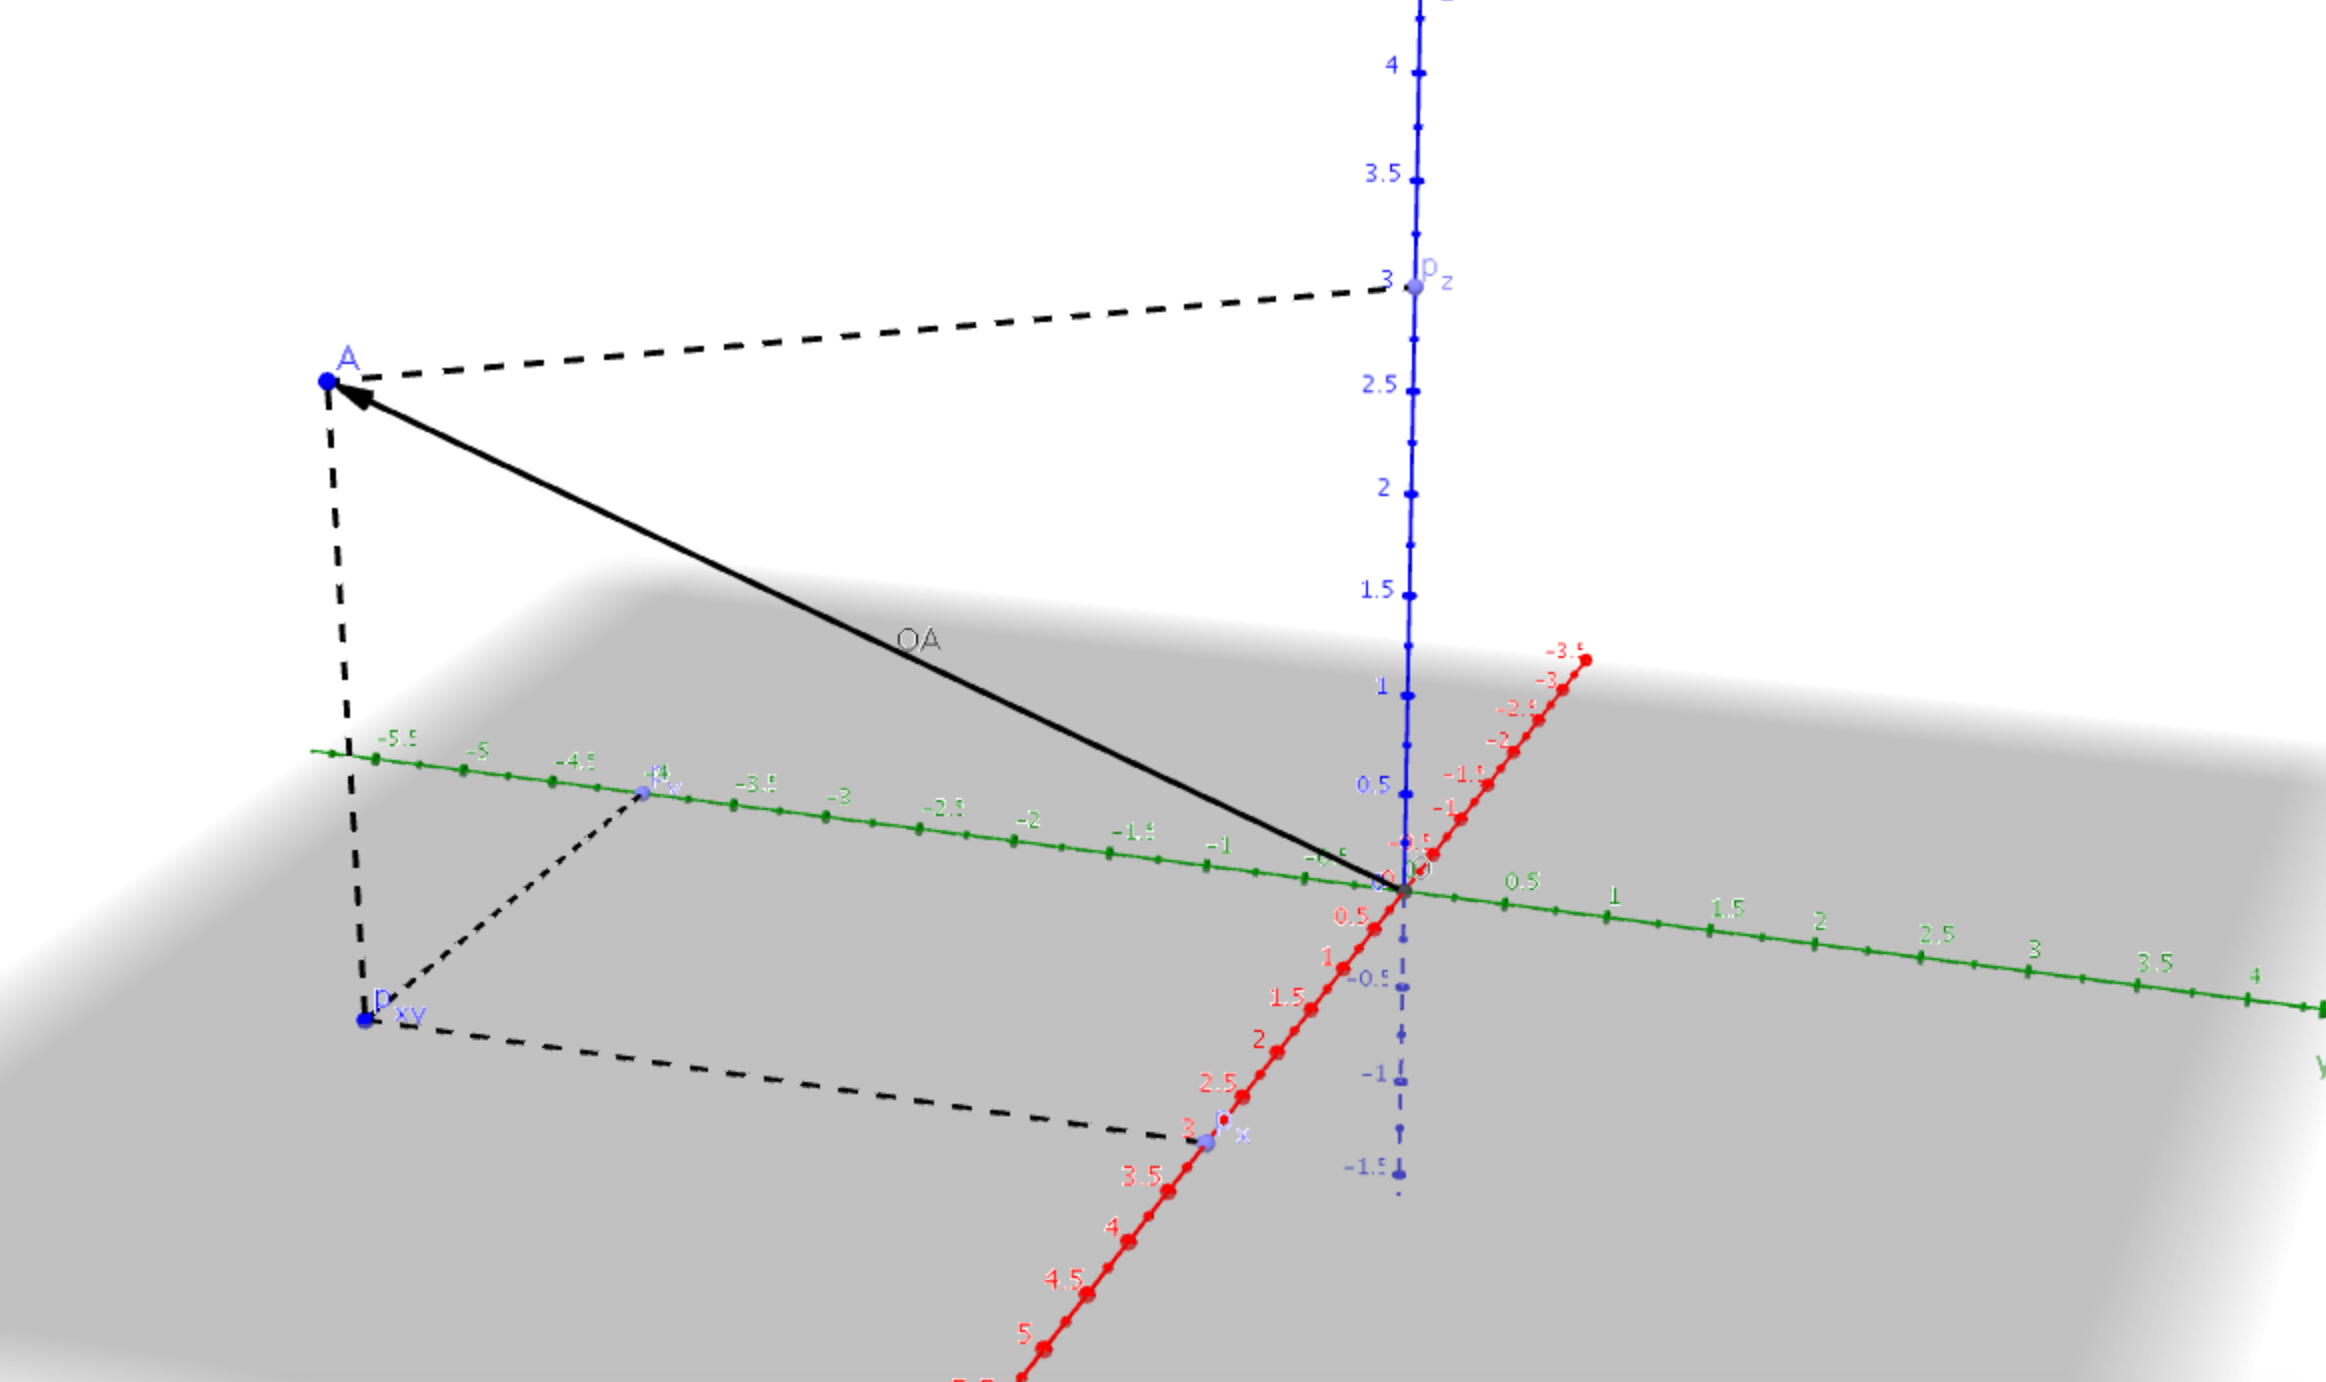
\includegraphics[width=10cm]{koordinaten3d.png}
\end{frame}

\begin{frame}{Schreibweise}
	\begin{bemerkung}[Koordinaten]
		Die Koordinaten von Vektoren werden wie folgt bezeichnet:
		\[
			\vv{a} = \begin{pmatrix}
			a_x \\ a_y \\ a_z
				\end{pmatrix} = \begin{pmatrix}
				a_1 \\ a_2 \\ a_3
				\end{pmatrix} \in \mathbb{R}^3
		\]
		für dreidimensionale Vektoren beziehungsweise
				\[
				\vv{b} = \begin{pmatrix}
				b_x \\ b_y
				\end{pmatrix} = \begin{pmatrix}
				b_1 \\ b_2
				\end{pmatrix} \in \mathbb{R}^2
				\]
		wenn der Vektor nur zweidimensional ist.
				
	\end{bemerkung}
\end{frame}

\begin{frame}{Schreibweise}
	\begin{bemerkung}[Koordinaten]
		Ganz allgemein werden die Koordinaten von Vektoren auch in höheren Dimensionen wie folgt bezeichnet:
		\[
		\vv{a} = \begin{pmatrix}
		a_1 \\ a_2 \\ \vdots \\ a_n
		\end{pmatrix} \in \mathbb{R}^{n}
		\]
		für n-dimensionale Vektoren.
	\end{bemerkung}
\end{frame}


\begin{frame}{Gleichheit von Vektoren}
	\begin{bemerkung}[Gleichheit von Vektoren]
		Zwei Vektoren sind schon dann \textbf{gleich}, wenn Sie dieselbe Länge (Betrag) und dieselbe Richtung haben!
	\end{bemerkung}
		\definecolor{xdxdff}{rgb}{0.49019607843137253,0.49019607843137253,1.}
		\definecolor{qqqqff}{rgb}{0.,0.,1.}
		\definecolor{uuuuuu}{rgb}{0.26666666666666666,0.26666666666666666,0.26666666666666666}
		\begin{tikzpicture}[line cap=round,line join=round,>=triangle 45,x=0.85cm,y=1.0cm]
		\draw[->,color=black] (-2.18,0.) -- (9.286666666666669,0.);
		\foreach \x in {-2.,-1.,1.,2.,3.,4.,5.,6.,7.,8.,9.}
		\draw[shift={(\x,0)},color=black] (0pt,2pt) -- (0pt,-2pt) node[below] {\footnotesize $\x$};
		\draw[->,color=black] (0.,-3.6866666666666705) -- (0.,4.94);
		\foreach \y in {-3.,-2.,-1.,1.,2.,3.,4.}
		\draw[shift={(0,\y)},color=black] (2pt,0pt) -- (-2pt,0pt) node[left] {\footnotesize $\y$};
		\draw[color=black] (0pt,-10pt) node[right] {\footnotesize $0$};
		\clip(-2.18,-3.6866666666666705) rectangle (9.286666666666669,4.94);
		\draw [ultra thick, ->] (0.,0.) -- (2.,4.);
		\draw [ultra thick, ->] (2.,0.) -- (4.,4.);
		\begin{scriptsize}
		\draw [fill=uuuuuu] (0.,0.) circle (1.5pt);
		\draw[color=qqqqff] (0.3,0.19333333333333036) node {$O$};
		\draw [fill=qqqqff] (2.,4.) circle (1.5pt);
		\draw[color=qqqqff] (2.3,4.193333333333331) node {$A$};
		\draw [fill=xdxdff] (2.,0.) circle (1.5pt);
		\draw[color=qqqqff] (2.3,0.19333333333333036) node {$B$};
		\draw [fill=qqqqff] (4.,4.) circle (1.5pt);
		\draw[color=qqqqff] (4.3,4.193333333333331) node {$C$};
		\draw[color=black] (2.1,2.14) node {\large $\vv{u}=\begin{pmatrix} 2 \\ 4 \end{pmatrix}$};
		\draw[color=black] (4.8,2.14) node {\large $\vv{v}=\begin{pmatrix} 2 \\ 4 \end{pmatrix} = \vv{u}$};
		\end{scriptsize}
		\end{tikzpicture}
\end{frame}


\begin{frame}{Ortsvektoren}
	Einen Vektor, der vom Ursprung des Koordinatensystems $O$ zu einem Punkt $P=\begin{pmatrix}p_1 \\ p_2 \\ \vdots \\ p_n \end{pmatrix}$ gerichtet ist, bezeichnet man als \textbf{Ortsvektor des Punktes $P$} und schreibt:
	\[
		\vv{OP} = \begin{pmatrix}
		p_1 \\ p_2 \\ \vdots \\ p_n
		\end{pmatrix}
	\]
	Die Bezeichnung $\begin{pmatrix}
	p_1 \\ p_2 \\ \vdots \\ p_n
	\end{pmatrix}$
	steht also sowohl für den Punkt $P$ als auch für den Ortsvektor dieses Punktes.
\end{frame}


\begin{frame}{Summe und Differenz von Vektoren}
	Vektoren werden koordinatenweise addiert bzw. subtrahiert:
	\[
	\vv{a} + \vv{b} = \begin{pmatrix} a_x \\ a_y \\ a_z
	\end{pmatrix} + \begin{pmatrix} b_x \\ b_y \\ b_z
	\end{pmatrix} = \begin{pmatrix} a_x + b_x \\ a_y + b_y \\ a_z + b_z
	\end{pmatrix}
	\]
		\[
		\vv{a} - \vv{b} = \begin{pmatrix} a_x \\ a_y \\ a_z
		\end{pmatrix} - \begin{pmatrix} b_x \\ b_y \\ b_z
		\end{pmatrix} = \begin{pmatrix} a_x - b_x \\ a_y - b_y \\ a_z - b_z
		\end{pmatrix}
		\]
	und entsprechend für n-dimensionale Vektoren.	
\end{frame}

\begin{frame}{Summe und Differenz von Vektoren}
	
	\begin{displaymath}
		\vv{a} = \vv{u} - \vv{v} = \begin{pmatrix}
		2 \\ 1
		\end{pmatrix} - \begin{pmatrix}
		2 \\ 3
		\end{pmatrix} = \begin{pmatrix} 0 \\ -2
		\end{pmatrix}
		\end{displaymath}
		\begin{displaymath}
		\vv{w} = \vv{u} + \vv{v} = \begin{pmatrix}
		2 \\ 1
		\end{pmatrix} + \begin{pmatrix}
		2 \\ 3
		\end{pmatrix} = \begin{pmatrix} 4 \\ 4
		\end{pmatrix}
	\end{displaymath}
\definecolor{qqqqff}{rgb}{0.,0.,1.}
\definecolor{uuuuuu}{rgb}{0.26666666666666666,0.26666666666666666,0.26666666666666666}
\begin{tikzpicture}[line cap=round,line join=round,>=triangle 45,x=0.9cm,y=1.0cm]
\draw[->,color=black] (-1.3577777777777764,0.) -- (9.486666666666665,0.);
\foreach \x in {-1.,-0.5,0.5,1.,1.5,2.,2.5,3.,3.5,4.,4.5,5.,5.5,6.,6.5,7.,7.5,8.,8.5,9.}
\draw[shift={(\x,0)},color=black] (0pt,2pt) -- (0pt,-2pt) node[below] {\footnotesize $\x$};
\draw[->,color=black] (0.,-1.262222222222225) -- (0.,4.995555555555551);
\foreach \y in {-1.,-0.5,0.5,1.,1.5,2.,2.5,3.,3.5,4.,4.5}
\draw[shift={(0,\y)},color=black] (2pt,0pt) -- (-2pt,0pt) node[left] {\footnotesize $\y$};
\draw[color=black] (0pt,-10pt) node[right] {\footnotesize $0$};
\clip(-1.3577777777777764,-1.262222222222225) rectangle (9.486666666666665,4.995555555555551);
\draw [ultra thick, ->] (0.,0.) -- (2.,1.);
\draw [ultra thick, ->] (0.,0.) -- (2.,3.);
\draw [ultra thick, ->] (2.,1.) -- (4.,4.);
\draw [ultra thick, ->] (2.,3.) -- (2.,1.);
\begin{scriptsize}
\draw [fill=uuuuuu] (0.,0.) circle (1.5pt);
\draw[color=uuuuuu] (0.06444444444444544,0.12444444444444139) node {$A$};
\draw [fill=qqqqff] (2.,1.) circle (1.5pt);
\draw[color=qqqqff] (2.064444444444445,1.1288888888888857) node {$B$};
\draw[color=black] (1.1066666666666675,0.8044444444444413) node {$\vv{u}$};
\draw[ultra thick, ->] (0., 0.) -- (4.,4.);
\draw[color=black] (2.5, 2.7) node {$\vv{w}$};
\draw [fill=qqqqff] (2.,3.) circle (1.5pt);
\draw[color=qqqqff] (2.064444444444445,3.128888888888885) node {$C$};
\draw[color=black] (1.1977777777777785,1.5911111111111078) node {$\vv{v}$};
\draw [fill=qqqqff] (4.,4.) circle (1.5pt);
\draw[color=qqqqff] (4.064444444444445,4.12444444444444) node {$D$};
\draw[color=black] (3.1977777777777783,2.595555555555552) node {$\vv{v}$};
\draw[color=black] (1.7555555555555562,2.08) node {$\vv{a}$};
\end{scriptsize}
\end{tikzpicture}
%\begin{tikzpicture}
%\begin{axis}[title=Differenz zweier Vektoren]
%\addplot[blue,
%quiver={u=\thisrow{u},v=\thisrow{v}},-stealth,ultra thick]
%table[row sep=\\]
%{
%x y u v
%0 0 1 0\\
%0 0 1 0\\
%0 0 0 1\\
%0 1 1 -1\\
%};
%\end{axis}
%\end{tikzpicture}
\end{frame}

\begin{frame}{Vektoren 3-dimensional}
	Dasselbe gilt natürlich auch für dreidimensionale Vektoren!
	\[
	\vv{u} + \vv{v} = \begin{pmatrix}
	0 \\ 1 \\ 2
	\end{pmatrix} + \begin{pmatrix}
	2 \\ 1 \\ 0
	\end{pmatrix} = \begin{pmatrix}
	2 \\ 2 \\ 2
	\end{pmatrix}
	\]
	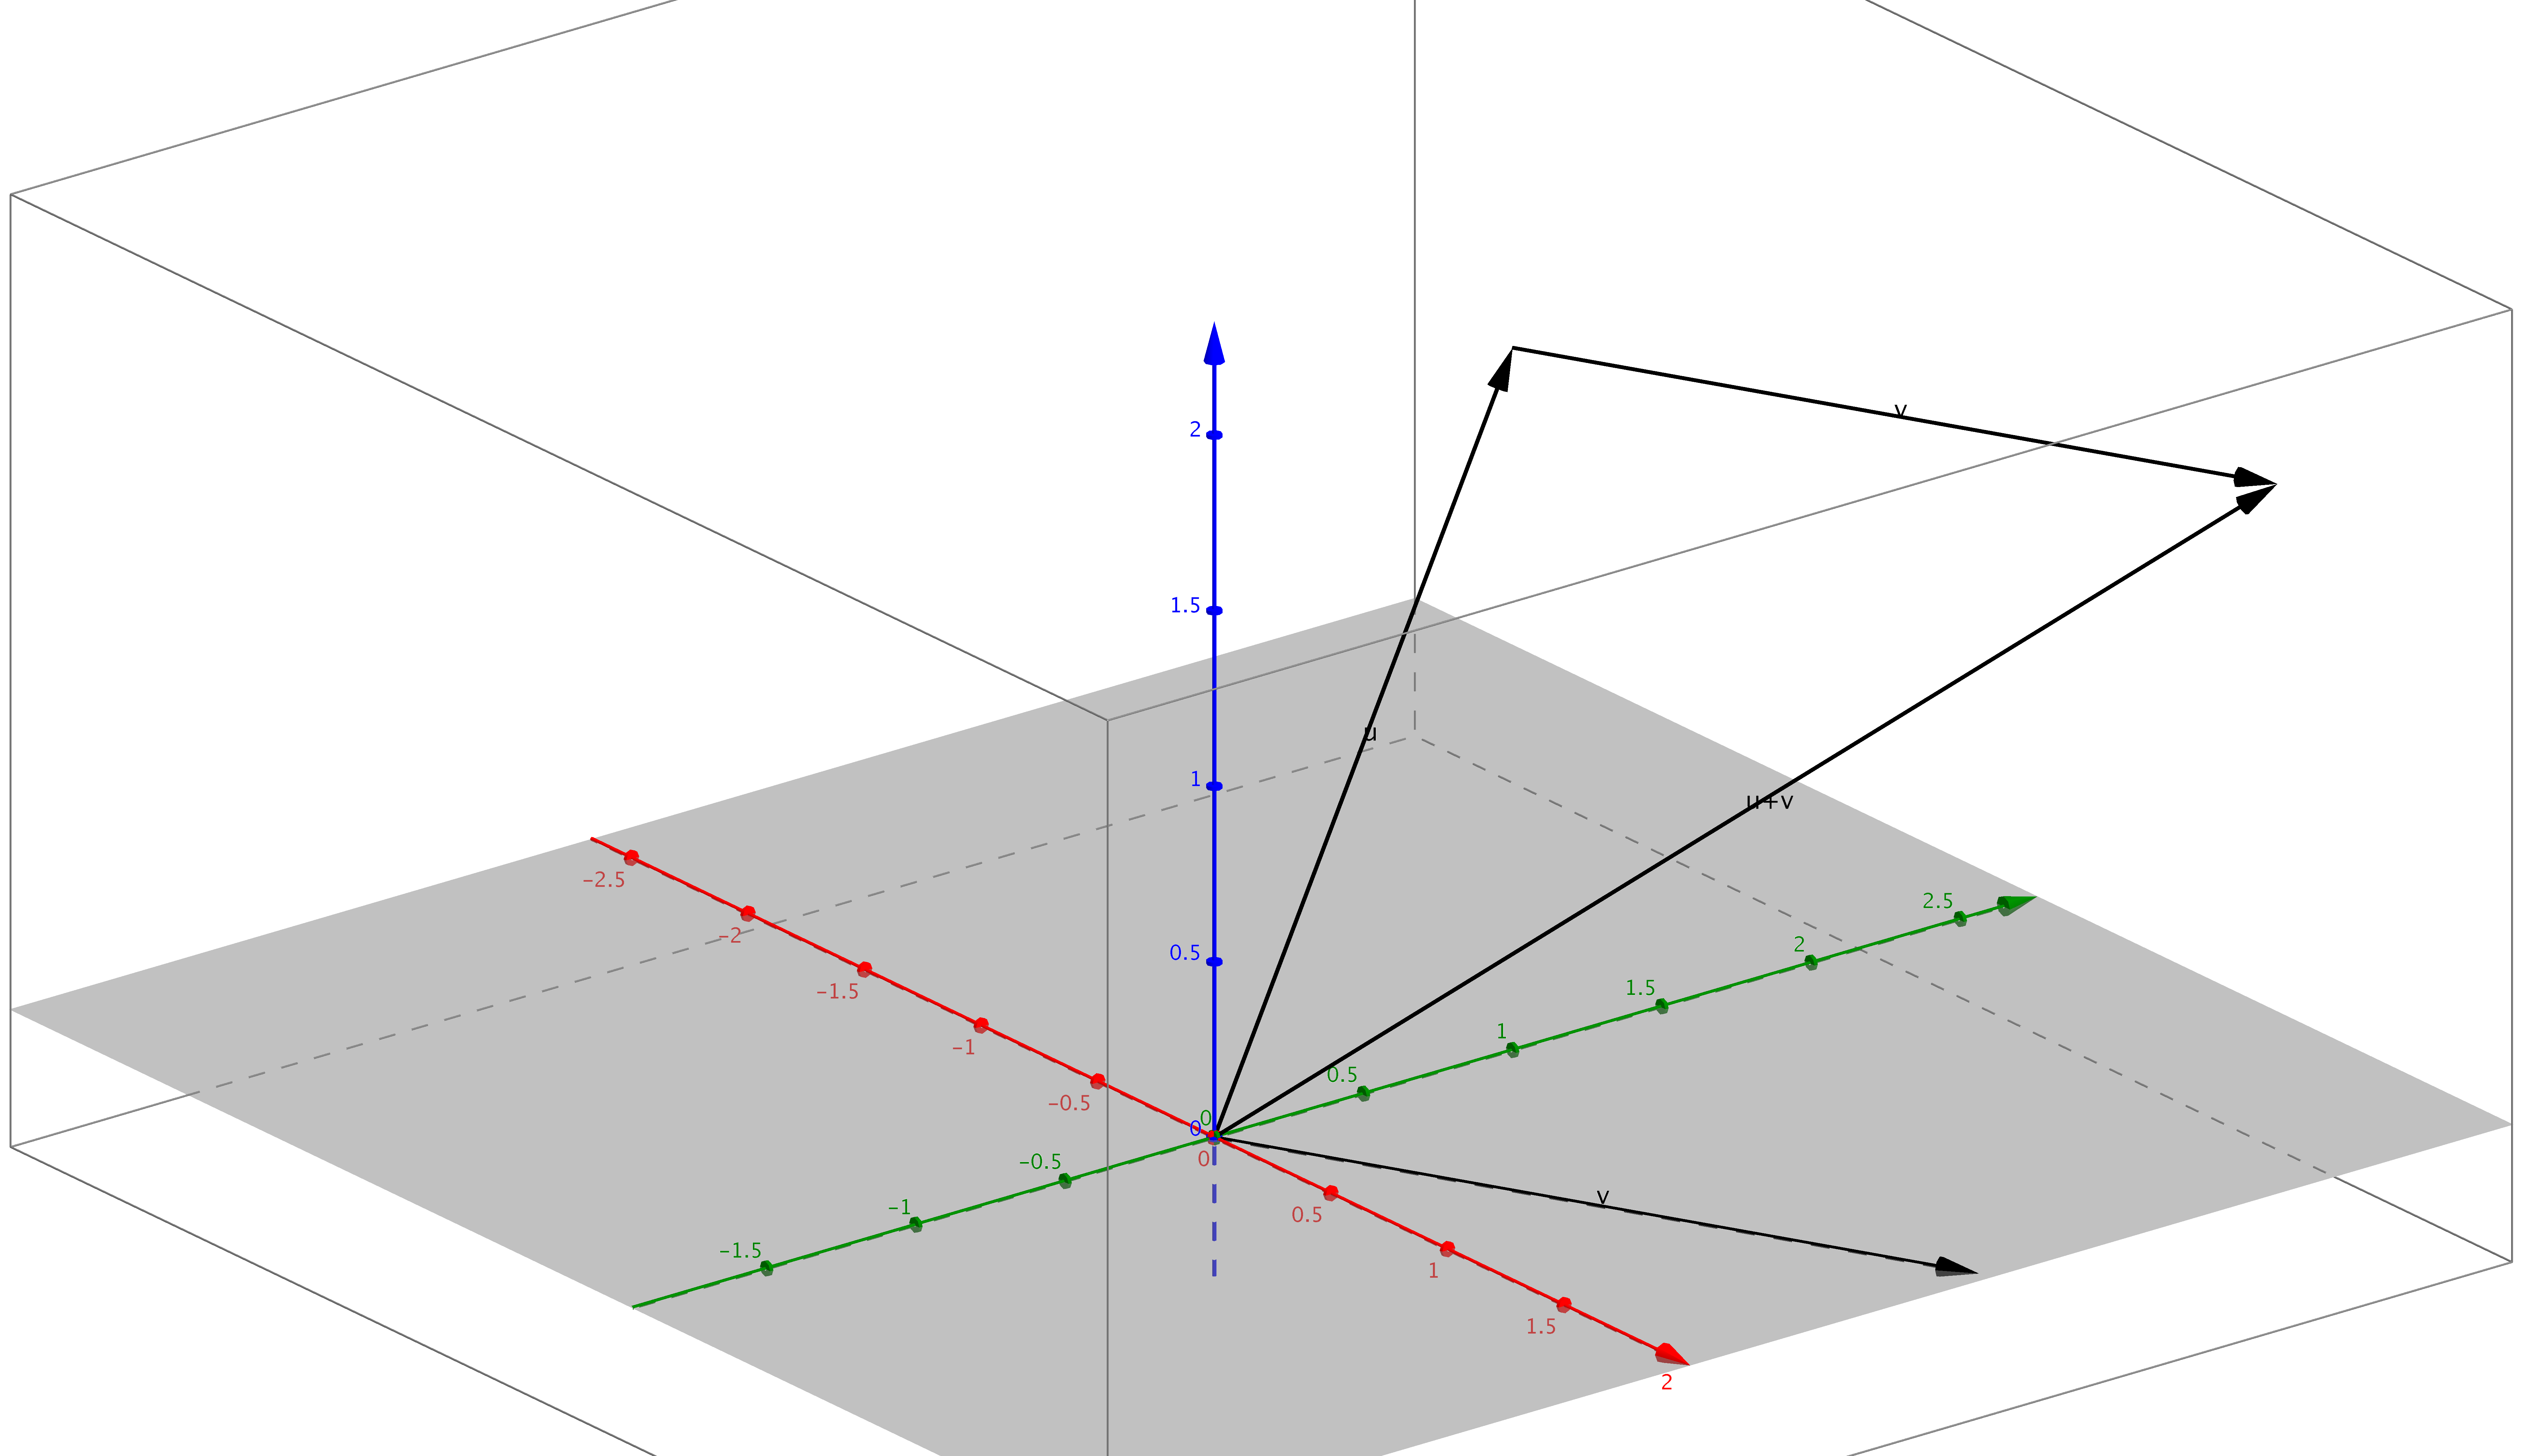
\includegraphics[width=10cm]{vektoren3d.png}
\end{frame}

\begin{frame}{Verlängern, Verkürzen und Umdrehen von Vektoren}
	Vektoren können mit Zahlen (Skalaren) multipliziert werden. Für eine Zahl $\lambda \in \mathbb{R}$ ist
	\[
		\lambda \vv{a} = \lambda \begin{pmatrix}a_x \\ a_y \\ a_z\end{pmatrix} = \begin{pmatrix}\lambda a_x \\ \lambda  a_y \\ \lambda a_z\end{pmatrix}
	\]
	und wieder entsprechend für n-dimensionale Vektoren.
\end{frame}

\begin{frame}{Multiplikation eines Vektors mit einem Skalar}
	Dabei gilt
	\begin{itemize}
	\item für $ | \lambda | > 1$ wird der Vektor verlängert/gestreckt.
	\item für $| \lambda |< 1$ wird der Vektor verkürzt/gestaucht.
	\item für $\lambda < 0$ wird die Richtung des Vektors zudem umgekehrt.
	\end{itemize}
	\definecolor{ffqqqq}{rgb}{1.,0.,0.}
	\definecolor{qqqqff}{rgb}{0.,0.,1.}
	\definecolor{uuuuuu}{rgb}{0.26666666666666666,0.26666666666666666,0.26666666666666666}
	\definecolor{cqcqcq}{rgb}{0.7529411764705882,0.7529411764705882,0.7529411764705882}
	\begin{tikzpicture}[line cap=round,line join=round,>=triangle 45,x=1.0cm,y=1.0cm]
	\draw [color=cqcqcq,, xstep=1.0cm,ystep=1.0cm] (-2.,-2.072292859071836) grid (7.,3.147259750704469);
	\draw[->,color=black] (-2.,0.) -- (7.,0.);
	\foreach \x in {-2.,-1.,1.,2.,3.,4.,5.,6.}
	\draw[shift={(\x,0)},color=black] (0pt,2pt) -- (0pt,-2pt) node[below] {\footnotesize $\x$};
	\draw[->,color=black] (0.,-2.072292859071836) -- (0.,3.147259750704469);
	\foreach \y in {-2.,-1.,1.,2.,3.}
	\draw[shift={(0,\y)},color=black] (2pt,0pt) -- (-2pt,0pt) node[left] {\footnotesize $\y$};
	\draw[color=black] (0pt,-10pt) node[right] {\footnotesize $0$};
	\clip(-2.,-2.072292859071836) rectangle (7.,3.147259750704469);
	\draw [->,line width=3.6pt] (0.,0.) -- (1.,2.);
	\draw [->,line width=1.2pt,color=ffqqqq] (0.,0.) -- (1.5,3.);
	\draw [->] (0.,0.) -- (-0.5,-1.);
	\begin{scriptsize}
	\draw [fill=uuuuuu] (0.,0.) circle (1.5pt);
	\draw[color=uuuuuu] (0.050538525269262585,0.1050062295777083) node {$O$};
	\draw [fill=qqqqff] (1.,2.) circle (1.5pt);
	\draw[color=qqqqff] (1.0497100248550122,2.1033492287492077) node {$A$};
	\draw[color=black] (1.1874067937033968,1.0892647217069542) node {$\vv{a}$};
	\draw [fill=qqqqff] (1.5,3.) circle (1.5pt);
	\draw[color=ffqqqq] (2.2900579950289974,2.3739374640433255) node {$\lambda \vv{a}$ für $\lambda = \frac{3}{2}$};
	\draw [fill=qqqqff] (-0.5,-1.) circle (1.5pt);
	\draw[color=qqqqff] (-0.4490472245236123,-0.8941652700080415) node {$C$};
	\draw[color=black] (1.0,-0.64677504631292964) node {$\lambda  \vv{a}$ für $\lambda = -\frac{1}{2}$ };
	\end{scriptsize}
	\end{tikzpicture}	
\end{frame}	

\subsubsection{Koordinaten}
\begin{frame}{Koordinatenvektoren}
	Die Vektoren der Länge 1 entlang der Koordinatenachsen haben eine spezielle Bezeichnung:
	\[
	\vv{e_x}=\begin{pmatrix} 1 \\ 0 \\ 0 \end{pmatrix} \quad 	\vv{e_y}=\begin{pmatrix} 0 \\ 1 \\ 0 \end{pmatrix} \quad
		\vv{e_z}=\begin{pmatrix} 0 \\ 0 \\ 1 \end{pmatrix}
	\]
	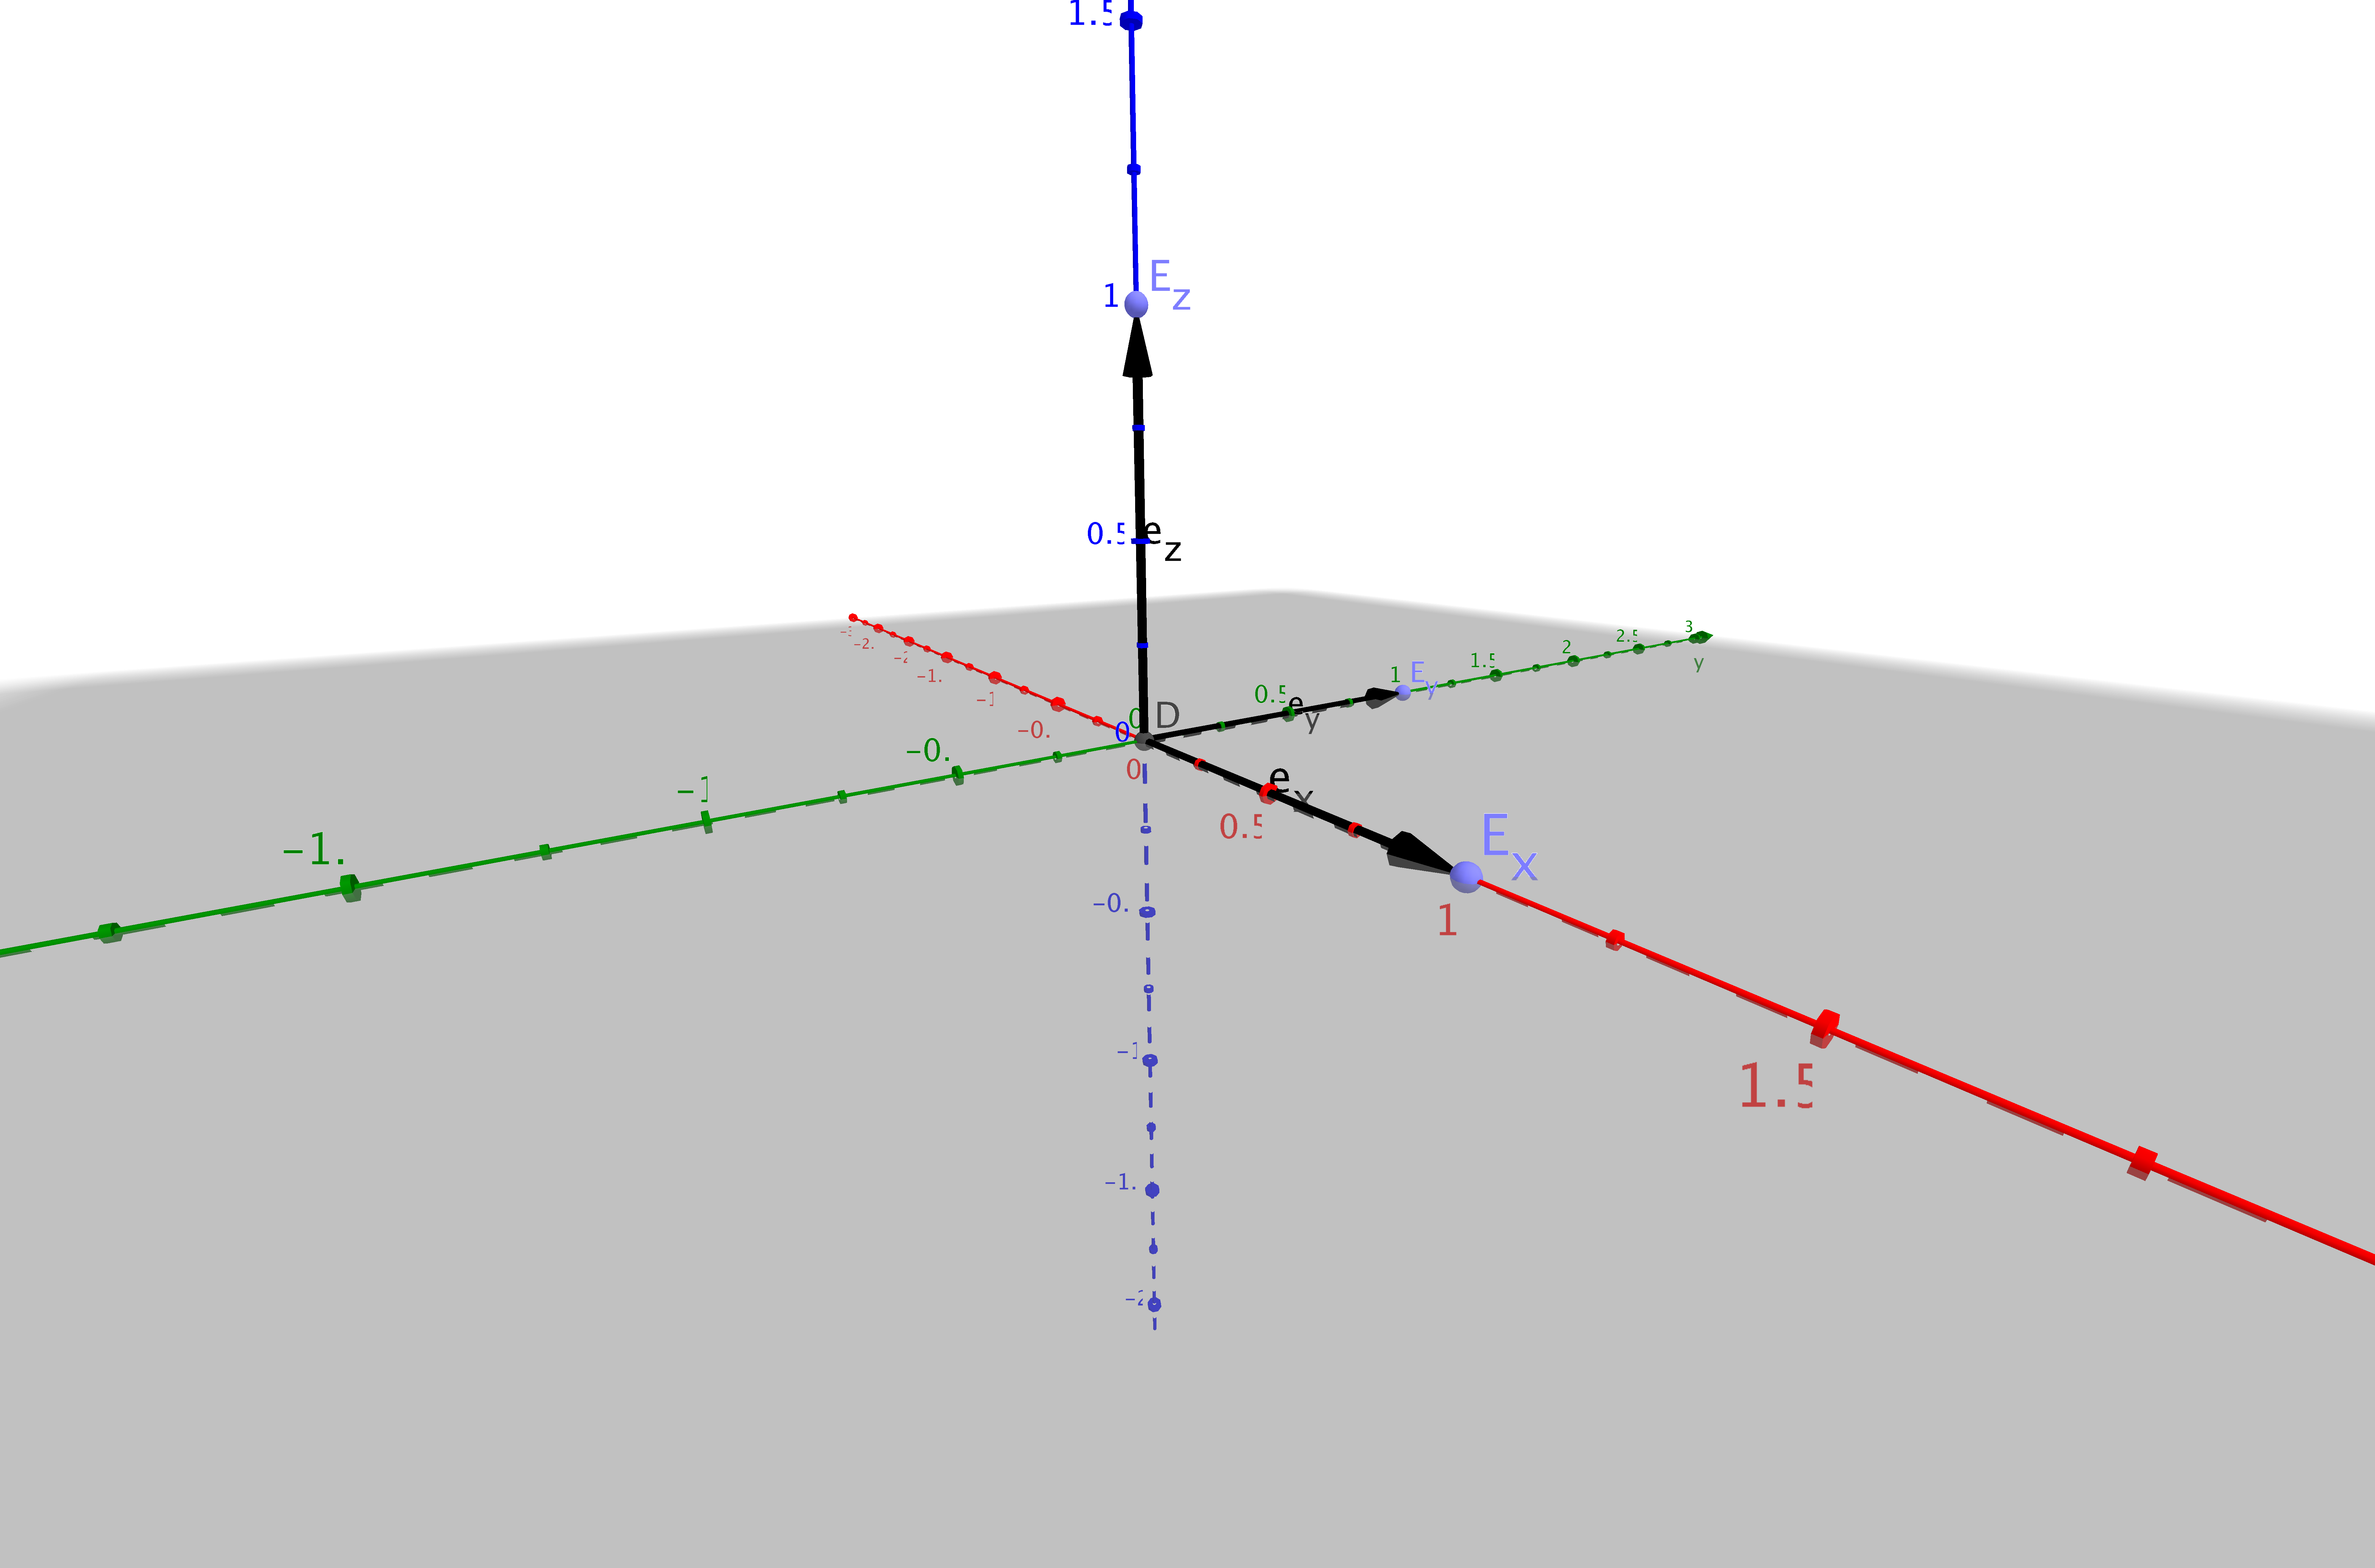
\includegraphics[width=10cm]{achsen.png}
\end{frame}

\begin{frame}{Projektionen}
	Mit Hilfe der Koordinatenvektoren kann man einen Vektor in seine Komponenten zerlegen:
	\[
	\begin{array}{cccc}
	\vv{OP} = \vv{a} = \begin{pmatrix}
	2 \\ 3 \\ 1
	\end{pmatrix} = &\underbrace{a_x \vv{e_x}} & + \underbrace{a_y \vv{e_y}}  + &\underbrace{a_z \vv{e_z}} \\
	&  \vv{a_x} & \vv{a_y} & \vv{a_z}
	\end{array}
	\]
	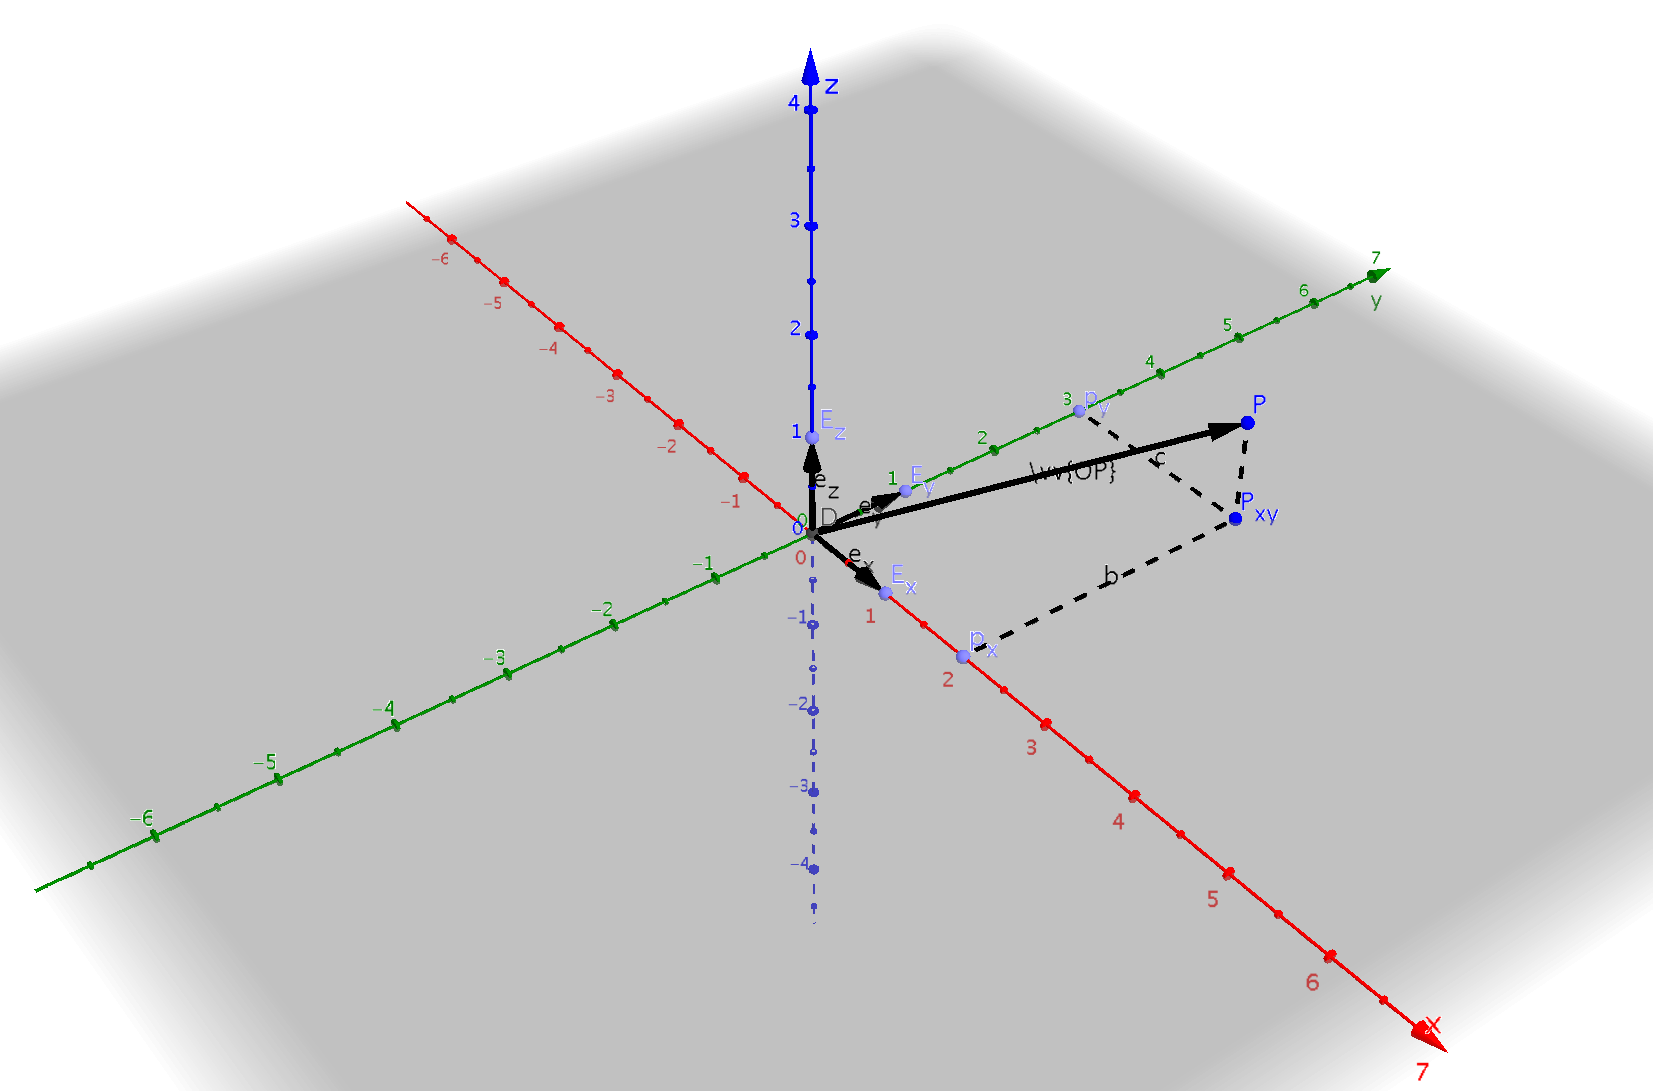
\includegraphics[width=10cm]{projektion.png}
\end{frame}

\subsubsection{Länge von Vektoren}
\begin{frame}{Länge eines Vektors 2-dimensional}
	Die Länge eines Vektors (seinen Betrag) kann man mit Hilfe des Satzes von Pythagoras bestimmen:
	\[
	\| \vv{a} \| = \sqrt{a_x^2 + a_y^2 } \qquad\text{für } \vv{a} = \begin{pmatrix}
	a_x \\ a_y
	\end{pmatrix}
	\]Also hier:	
	\[
	\| \vv{a} \| = \sqrt{3^2 + 4^2 } = \sqrt{9+16} = \sqrt{25} = 5 \qquad\text{für } \vv{a} = \begin{pmatrix}
	3 \\ 4
	\end{pmatrix}
	\]
%	\definecolor{ffzzqq}{rgb}{1.,0.6,0.}
\definecolor{ccwwqq}{rgb}{0.8,0.4,0.}
\definecolor{xdxdff}{rgb}{0.49019607843137253,0.49019607843137253,1.}
\definecolor{qqqqff}{rgb}{0.,0.,1.}
\definecolor{uuuuuu}{rgb}{0.26666666666666666,0.26666666666666666,0.26666666666666666}
\definecolor{cqcqcq}{rgb}{0.7529411764705882,0.7529411764705882,0.7529411764705882}
\begin{tikzpicture}[line cap=round,line join=round,>=triangle 45,x=1.0cm,y=1.0cm]
\draw [color=cqcqcq,, xstep=1.0cm,ystep=1.0cm] (-0.1303703703703693,-0.09925925925926203) grid (6.85037037037037,4.048888888888889);
\draw[->,color=black] (0.,0.) -- (6.85037037037037,0.);
\foreach \x in {,1.,2.,3.,4.,5.,6.}
\draw[shift={(\x,0)},color=black] (0pt,2pt) -- (0pt,-2pt) node[below] {\footnotesize $\x$};
\draw[->,color=black] (0.,0.) -- (0.,4.048888888888889);
\foreach \y in {,1.,2.,3.,4.}
\draw[shift={(0,\y)},color=black] (2pt,0pt) -- (-2pt,0pt) node[left] {\footnotesize $\y$};
\draw[color=black] (0pt,-10pt) node[right] {\footnotesize $0$};
\clip(-0.1303703703703693,-0.09925925925926203) rectangle (6.85037037037037,4.048888888888889);
\draw [->,line width=2.8pt] (0.,0.) -- (3.,4.);
\draw [line width=2.8pt,color=ccwwqq] (3.,4.)-- (3.,0.);
\draw [line width=2.8pt,color=ffzzqq] (3.,0.)-- (0.,0.);
\begin{scriptsize}
\draw [fill=uuuuuu] (0.,0.) circle (1.5pt);
\draw[color=uuuuuu] (0.04148148148148249,0.08444444444444182) node {$O$};
\draw [fill=qqqqff] (3.,4.) circle (1.5pt);
\draw[color=qqqqff] (3.04,4.001481481481482) node {$A$};
\draw[color=black] (2.0,2.0) node {$\vv{a}$};
\draw[color=black] (0.8,2.0) node {$\| \vv{a}\| = 5$};
\draw [fill=xdxdff] (3.,0.) circle (1.5pt);
\draw[color=xdxdff] (3.04,0.08444444444444182) node {$B$};
\draw[color=ccwwqq] (4.0044444444444447,2.0696296296296284) node {$a_y = 4$};
\draw[color=ffzzqq] (1.6,0.26148148148147892) node {$a_x = 3$};
\end{scriptsize}
\end{tikzpicture}
\definecolor{ffzzqq}{rgb}{1.,0.6,0.}
\definecolor{ccwwqq}{rgb}{0.8,0.4,0.}
\definecolor{xdxdff}{rgb}{0.49019607843137253,0.49019607843137253,1.}
\definecolor{qqqqff}{rgb}{0.,0.,1.}
\definecolor{uuuuuu}{rgb}{0.26666666666666666,0.26666666666666666,0.26666666666666666}
\definecolor{cqcqcq}{rgb}{0.7529411764705882,0.7529411764705882,0.7529411764705882}
\begin{tikzpicture}[line cap=round,line join=round,>=triangle 45,x=1.0cm,y=1.0cm]
\draw [color=cqcqcq,, xstep=1.0cm,ystep=1.0cm] (-0.1303703703703693,-0.09925925925926203) grid (6.85037037037037,4.048888888888889);
\draw[->,color=black] (0.,0.) -- (6.85037037037037,0.);
\foreach \x in {,1.,2.,3.,4.,5.,6.}
\draw[shift={(\x,0)},color=black] (0pt,2pt) -- (0pt,-2pt) node[below] {\footnotesize $\x$};
\draw[->,color=black] (0.,0.) -- (0.,4.048888888888889);
\foreach \y in {,1.,2.,3.,4.}
\draw[shift={(0,\y)},color=black] (2pt,0pt) -- (-2pt,0pt) node[left] {\footnotesize $\y$};
\draw[color=black] (0pt,-10pt) node[right] {\footnotesize $0$};
\clip(-0.1303703703703693,-0.09925925925926203) rectangle (6.85037037037037,4.048888888888889);
\draw [->,line width=2.8pt] (0.,0.) -- (3.,4.);
\draw [line width=2.8pt,color=ccwwqq] (3.,4.)-- (3.,0.);
\draw [line width=2.8pt,color=ffzzqq] (3.,0.)-- (0.,0.);
\begin{scriptsize}
\draw [fill=uuuuuu] (0.,0.) circle (1.5pt);
\draw[color=uuuuuu] (0.04148148148148249,0.08444444444444182) node {$O$};
\draw [fill=qqqqff] (3.,4.) circle (1.5pt);
\draw[color=qqqqff] (3.04,4.001481481481482) node {$A$};
\draw[color=black] (2.0,2.0) node {$\vv{a}$};
\draw[color=black] (0.8,2.0) node {$\| \vv{a}\| = 5$};
\draw [fill=xdxdff] (3.,0.) circle (1.5pt);
\draw[color=xdxdff] (3.04,0.08444444444444182) node {$B$};
\draw[color=ccwwqq] (4.0044444444444447,2.0696296296296284) node {$a_y = 4$};
\draw[color=ffzzqq] (1.6,0.26148148148147892) node {$a_x = 3$};
\end{scriptsize}
\end{tikzpicture}	
\end{frame}

\begin{frame}{Länge eines Vektors 3-dimensional}
	Die Betrag eines dreidimensionalen Vektors kann man ebenfalls mit Hilfe des Satzes von Pythagoras bestimmen:
	\[
	\| \vv{a} \| = \sqrt{a_x^2 + a_y^2 + a_z^2} \qquad\text{für } \vv{a} = \begin{pmatrix}
	a_x \\ a_y \\ a_z
	\end{pmatrix}
	\]
\end{frame}
\begin{frame}{Länge eines Vektors 3-dimensional}		
	\[
	\| \vv{a} \| = \sqrt{3^2 + 4^2 + 5^2} = \sqrt{50} = 7.0710... \qquad\text{für } \vv{a} = \begin{pmatrix}
	3 \\ 4 \\ 5
	\end{pmatrix}
	\]
	denn $a_{xy} = \sqrt{3^2 + 4^2}$ und $\|\vv{a}\| = \sqrt{a_{xy}^2 + a_z^2}$
	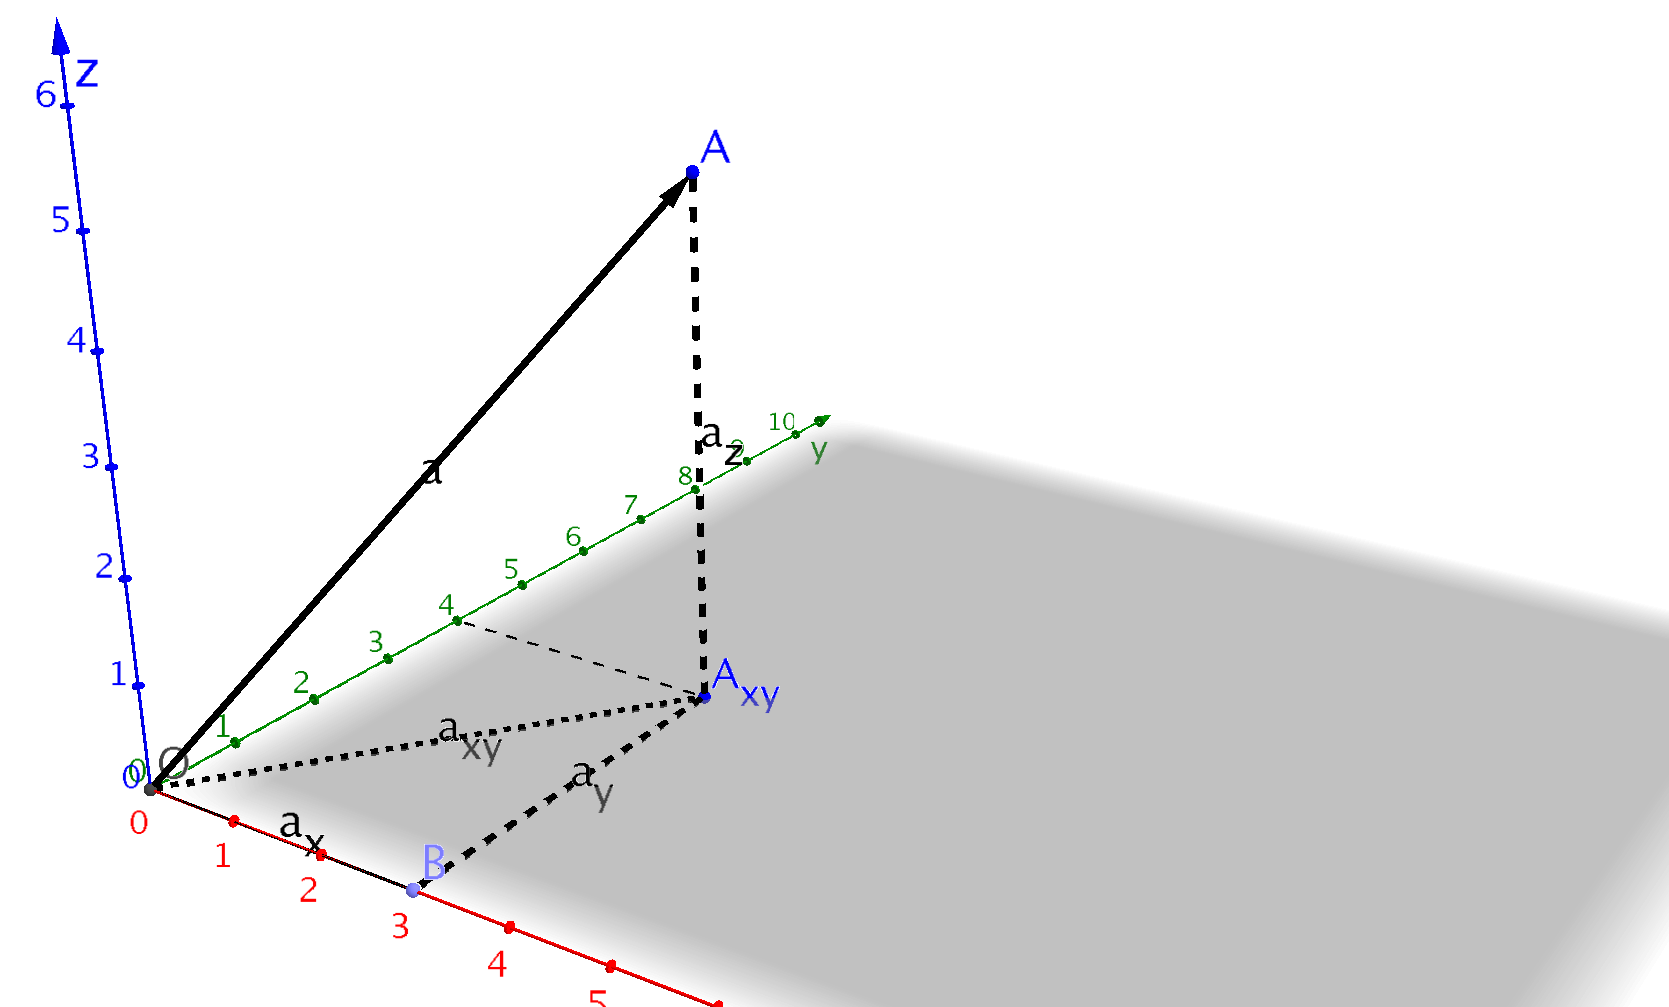
\includegraphics[width=10cm]{laengevektor3d.png}	
\end{frame}

\begin{frame}{Länge eines Vektors n-dimensional}
	Entsprechend gilt für die Länge n-dimensionaler Vektoren
	\[
	\| \vv{a} \| := \sqrt{a_1^2 + a_2^2 + \ldots + a_n^2}
	\]	
\end{frame}

\subsubsection{Skalarprodukt}
\begin{frame}{Produkte von Vektoren}
	Es gibt auch Produkte, an denen zwei Vektoren oder drei Vektoren beteiligt sind:
	\begin{itemize}
		\item \textbf{Skalarprodukt}
		
		 $\vv{a} \cdot \vv{b} \in \mathbb{R}$
		
		Das Ergebnis ist ein Skalar, also eine reelle Zahl
		\item \textbf{Vektor}- oder \textbf{Kreuzprodukt}
		
		$\vv{a} \times \vv{b} \in \mathbb{R}^3$
		
		Das Ergebnis ist ein (3-dimensionaler) Vektor.
		\item \textbf{Spatprodukt}
		
		$\left< \vv{a}, \vv{b}, \vv{c} \right> := \vv{a} \cdot (\vv{b} \times \vv{c} ) \in \mathbb{R}$
		
		Das Ergebnis ist eine Zahl, die das Volumen des von den drei Vektoren aufgespannten Spates ergibt.
	\end{itemize}	
\end{frame}


\begin{frame}{Skalarprodukt}
	\begin{definition}[Skalarprodukt]
		Das Skalarprodukt zweier Vektoren $\vv{a}$ und $\vv{b}$ ist definiert als
		\[
		\vv{a} \cdot \vv{b} := \begin{pmatrix}
		a_1 \\ a_2 \\ \vdots \\ a_n
		\end{pmatrix} \cdot
		\begin{pmatrix}
		b_1 \\ b_2 \\ \vdots \\ b_n
		\end{pmatrix} := a_1 b_1 + a_2 b_2  + \ldots + a_n b_n
		\]
	\end{definition}
	\begin{bemerkung}
		Die Komponenten werden also paarweise multipliziert und die Produkte addiert.
	\end{bemerkung}
\end{frame}

\begin{frame}{Skalarprodukt - Geometrische Bedeutung}
\begin{theorem}
	Für den zwischen zwei Vektoren $\vv{a}$ und $\vv{b}$ eingeschlossenen Winkel $\alpha$ gilt:
	\[
	\vv{a} \cdot \vv{b} = \| \vv{a} \| \| \vv{b} \| \cos \alpha
 \iff \cos \alpha = \frac{\vv{a}\cdot \vv{b}}{\| \vv{a} \| \| \vv{b} \| }	\]
	wobei $0 \leq \alpha \leq 180^\circ$.
\end{theorem}
\definecolor{qqwuqq}{rgb}{0.,0.39215686274509803,0.}
\definecolor{qqqqff}{rgb}{0.,0.,1.}
\definecolor{uuuuuu}{rgb}{0.26666666666666666,0.26666666666666666,0.26666666666666666}
\definecolor{cqcqcq}{rgb}{0.7529411764705882,0.7529411764705882,0.7529411764705882}
\begin{tikzpicture}[line cap=round,line join=round,>=triangle 45,x=1.0cm,y=1.0cm]
\draw [color=cqcqcq,, xstep=1.0cm,ystep=1.0cm] (-0.22494,-0.1387654320987674) grid (4.428888888888889,2.6266666666666683);
\draw[->,color=black] (-0.22494,0.) -- (4.428888888888889,0.);
\foreach \x in {,1.,2.,3.,4.}
\draw[shift={(\x,0)},color=black] (0pt,2pt) -- (0pt,-2pt) node[below] {\footnotesize $\x$};
\draw[->,color=black] (0.,-0.1387654320987674) -- (0.,2.6266666666666683);
\foreach \y in {,1.,2.}
\draw[shift={(0,\y)},color=black] (2pt,0pt) -- (-2pt,0pt) node[left] {\footnotesize $\y$};
\draw[color=black] (0pt,-10pt) node[right] {\footnotesize $0$};
\clip(-0.22494,-0.1387654320987674) rectangle (4.428888888888889,2.6266666666666683);
\draw [shift={(0.,0.)},color=qqwuqq,fill=green,fill opacity=2] (0,0) -- (0.:1) arc (0.:63.43494882292201:1) -- cycle;
\draw [->,line width=2.pt] (0.,0.) -- (1.,2.);
\draw [->,line width=2.pt] (0.,0.) -- (2.,0.);
\begin{scriptsize}
\draw [fill=uuuuuu] (0.,0.) circle (1.5pt);
\draw [fill=qqqqff] (1.,2.) circle (1.5pt);
\draw[color=qqqqff] (1.0274061441237503,2.053827160493828) node {$B$};
\draw[color=black] (0.4940726127145822,1.0424691358024687) node {$a$};
\draw [fill=qqqqff] (2.,0.) circle (1.5pt);
\draw[color=qqqqff] (2.026912688172043,0.054814814814813095) node {$C$};
\draw[color=black] (1.0116036691190342,0.050864197530862465) node {$b$};
\draw[color=qqwuqq] (1.22147991888322963,0.250864197530862465) node {$\alpha = 63.43\textrm{\degre}$};
\end{scriptsize}
\end{tikzpicture}

Insbesondere ist
	$
	\| \vv{a} \| = \sqrt{ \vv{a} \cdot \vv{a} }
	$
\end{frame}



\begin{frame}{Skalarprodukt - Rechenregeln}
	\begin{theorem}	
		Für das Skalarprodukt gilt \textbf{das Kommutativ-Gesetz}
		\[
			\vv{a} \cdot \vv{b} = \vv{b} \cdot \vv{a}
		\]
		als auch \textbf{das Distributiv-Gesetz}
		\[
			\vv{a} \cdot \left( \vv{b} + \vv{c} \right) = \vv{a} \cdot \vv{b} + \vv{a} \cdot \vv{c} \mbox{ und } \left( \lambda \vv{a} \right) \cdot \vv{b} = \lambda \left( \vv{a} \cdot \vv{b} \right)
 		\]
		
		Zudem sind zwei Vektoren $\vv{a}$ und $\vv{b}$ senkrecht aufeinander genau dann, wenn $\vv{a}\cdot\vv{b}=0$:
		\[
		\vv{a} \perp \vv{b} \Leftrightarrow \vv{a} \cdot \vv{b} = 0
		\]
	\end{theorem}	
\end{frame}

\begin{frame}{Kosinussatz}
	\begin{theorem}
		Für zwei Vektoren $\vv{a}$ und $\vv{b}$ gilt:
		\[
		\| \vv{a} - \vv{b}\|^2 = \|\vv{a}\|^2 + \|\vv{b}\|^2 - 2 \vv{a} \cdot \vv{b}
		\]
	\end{theorem}
	\begin{bemerkung}
		Dieser Satz ist der aus der Schule bekannte Kosinussatz:
		\[
			c^2 = a^2 + b^2 - 2 a b \cos \gamma
		\]
		wobei $\gamma$ der Winkel zwischen den Seiten $a$ und $b$ ist, denn
		\[
		\vv{a} \cdot \vv{b} = \| \vv{a} \| \| \vv{b} \| \cos \gamma
		\]
		Für $\vv{a} \perp \vv{b}$ ist das der Satz des Pythagoras:
		\[
			\left\| \vv{a} - \vv{b} \right\|^2 = \|\vv{a}\|^2 + \|\vv{b}\|^2
		\]
	\end{bemerkung}
\end{frame}

\begin{frame}{Cauchy-Schwarzsche Ungleichung}
	\begin{theorem}
		Für das Skalarprodukt gilt die Ungleichung:
		\[
			| \vv{a} \cdot \vv{b} | \leq \|\vv{a}\| \|\vv{b}\|
		\]
		für beliebige Vektoren $\vv{a}$ und $\vv{b}$.
	\end{theorem}
	Irgendwie klar, weil $|\cos \gamma| \leq 1$ für beliebige Winkel $\gamma$.
\end{frame}

\begin{frame}{Skalarprodukt - Anwendungsbeispiel}
	Greift eine konstante Kraft $\vv{F}$  an einem Massepunkt $M$ an und verschiebt ihn dabei um die Strecke $\vv{s}$, so gilt für die am Massepunkt $M$ geleistete Arbeit $W$ (das ist ein Skalar!)
	\[
		W = \vv{F} \cdot \vv{s} = \| \vv{F} \| \| \vv{s} \| \cos \alpha = \| \vv{F_s}\| \|\vv{s}\|
	\]
	wobei $\alpha$ der Winkel zwischen der Richtung der Kraft $\vv{F}$ und der Bewegungsrichtung $\vv{s}$ und $\vv{F_s} := \frac{\vv{F} \cdot \vv{s}}{\|\vv{s}\|} \frac{\vv{s}}{\|\vv{s}\|} = \left(\vv{F} \cdot \vv{e_s} \right) \vv{e_s}$ ist.
\definecolor{ffzztt}{rgb}{1.,0.6,0.2}
\definecolor{qqwuqq}{rgb}{0.,0.39215686274509803,0.}
\definecolor{ffqqtt}{rgb}{1.,0.,0.2}
\definecolor{qqqqff}{rgb}{0.,0.,1.}
\begin{tikzpicture}[line cap=round,line join=round,>=triangle 45,x=1.2cm,y=1.2cm]
\clip(0.9985185185185195,1.4340740740740714) rectangle (8.305185185185188,5.582222222222217);
\draw [shift={(2.,2.)},color=yellow,fill=green,fill opacity=0.1] (0,0) -- (0.:0.5777777777777778) arc (0.:36.86989764584402:0.5777777777777778) -- cycle;
\draw [->,color=ffqqtt] (2.,2.) -- (4.,2.);
\draw [->] (2.,2.) -- (6.,5.);
\draw [line width=1.pt,dotted] (6.,5.)-- (6.,2.);
\draw [->,color=ffzztt] (2.,2.) -- (6.,2.);
\begin{scriptsize}
\draw [fill=qqqqff] (2.,2.) circle (0.5pt);
\draw[color=qqqqff] (2.0414814814814823,2.285925925925923) node {$M$};
\draw [fill=qqqqff] (6.,5.) circle (0.5pt);
\draw [fill=qqqqff] (4.,2.) circle (0.5pt);
\draw[color=ffqqtt] (3.0133333333333345,2.1740740740740713) node {$\vv{s}$};
\draw[color=black] (4.002962962962964,3.767407407407404) node {$\vv{F}$};
\draw[color=qqwuqq] (2.3837037037037046,2.1562962962962934) node {$\alpha$};
\draw [fill=qqqqff] (6.,2.) circle (0.5pt);
\draw[color=ffzztt] (4.026666666666667,2.2918518518518487) node {$\vv{F_s}$};
\end{scriptsize}
\end{tikzpicture}
\end{frame}

\subsubsection{Vektorprodukt}
\begin{frame}{Vektorprodukt / Kreuzprodukt / äußeres Produkt}
	Für zwei \textbf{dreidimensionale} Vektoren
	\[
	\vv{a} = \begin{pmatrix}
	a_x \\ a_y \\ a_z
	\end{pmatrix} \mbox{ und } 	\vv{b} = \begin{pmatrix}
	b_x \\ b_y \\ b_z
	\end{pmatrix}
 	\]
 	ist das \textbf{Kreuzprodukt} (auch \textbf{Vektorprodukt} oder \textbf{äußeres Produkt}) definiert als
 	\[
	 	\vv{a} \times \vv{b} := \begin{pmatrix}
	 	a_y b_z - a_z b_y \\
	 	a_z b_x - a_x b_z \\
	 	a_x b_y - a_y b_x
	 	\end{pmatrix} \in \mathbb{R}^3
 	\]
\end{frame}

\begin{frame}{Eigenschaften des Vektorproduktes}
	Für beliebige Vektoren $\vv{a} \in \mathbb{R}^3$, $\vv{b} \in \mathbb{R}^3$ und $\vv{c} \in \mathbb{R}^3$ und beliebiges $\lambda \in \mathbb{R}$ gilt:
	\[	\vv{a}, \vv{b} \mbox{ und } \vv{a}  \times  		\vv{b}  \mbox{ bilden ein Rechts-System}
	\]
	\begin{align*}
		\vv{a} \times \vv{b} & =  - \vv{b} \times \vv{a} \\
		\left( \lambda \vv{a} \right) \times \vv{b} & =  \vv{a} \times \left( \lambda \vv{b} \right) = \lambda \left( \vv{a} \times \vv{b} \right)  \\
		\vv{a} \times \left( \vv{b} + \vv{c} \right) & =   \vv{a} \times \vv{b} + \vv{a} \times \vv{c} \\
		\vv{a} \times \vv{b} = \vv{0} &  \Leftrightarrow  \vv{a} \| \vv{b}  \\
		\left(\vv{a} \times \vv{b}\right) \perp \vv{a} & \mbox{ und }  \left(\vv{a} \times \vv{b}\right) \perp \vv{b} \\
		\left\| \vv{a} \times \vv{b} \right\| & =  \|\vv{a}\| \|\vv{b}\| \sin \alpha
	\end{align*}
	wobei $0 \leq \alpha \leq 180^\circ$ der von $\vv{a}$ und $\vv{b}$ eingeschlossene Winkel ist.
\end{frame}

\begin{frame}{Kreuzprodukt - Beispiel}
	
	\begin{align*}
	\begin{pmatrix}
	1 \\ 0 \\ 0
	\end{pmatrix} \times  \begin{pmatrix}
	0 \\ 1 \\ 0
	\end{pmatrix} & = \begin{pmatrix}
	0 \cdot 0 - 0 \cdot 1 \\
	0 \cdot 0 - 1 \cdot 0 \\
	1 \cdot 1 - 0 \cdot 0	
	\end{pmatrix} = \begin{pmatrix}
	0 \\ 0 \\ 1
	\end{pmatrix} \\
	\begin{pmatrix}
	1 \\ 0 \\ 0
	\end{pmatrix} \times  \begin{pmatrix}
	1 \\ 1 \\ 0
	\end{pmatrix} & = \begin{pmatrix}
	0 \cdot 0 - 0 \cdot 1 \\
	0 \cdot 1 - 1 \cdot 0 \\
	1 \cdot 1 - 0 \cdot 1	
	\end{pmatrix} = \begin{pmatrix}
	0 \\ 0 \\ 1
	\end{pmatrix} \\
	\begin{pmatrix}
		1 \\ 0 \\ 3
	\end{pmatrix} \times  \begin{pmatrix}
	2 \\ -3 \\ 4
	\end{pmatrix} & = \begin{pmatrix}
	0 \cdot 4 - 3 \cdot (-3) \\
	3 \cdot 2 - 1 \cdot 4 \\
	1 \cdot -3 - 0 \cdot 2	
	\end{pmatrix} = \begin{pmatrix}
	9 \\ 2 \\ -3
	\end{pmatrix}
	\end{align*}
{\scriptsize 	%\href{/Users/stefan/sciebo/Mathematik/EigeneVorlesung/Folien/kreuzprodukt.ggb}{Beispiel Kreuzprodukt Geogebra}
\href{https://fh-swf.sciebo.de/public.php?service=files&t=83c3e87e19f49991d0d6c55da10f8c7d}{Beispiel Kreuzprodukt Geogebra}
}\end{frame}

\begin{frame}{Kreuzprodukt - Anwendungen}
	Das von zwei Vektoren $\vv{a}$ und $\vv{b}$ aufgespannte Parallelogramm hat den Flächeninhalt
	\[
		\| \vv{a} \times \vv{b}\| = \left|  \|\vv{a}\| \|\vv{b}\| \sin \alpha \right|
	\]
	\href{/Users/stefan/sciebo/Mathematik/EigeneVorlesung/Folien/parallelogramm.ggb}{Parallelogramm-Beispiel}
	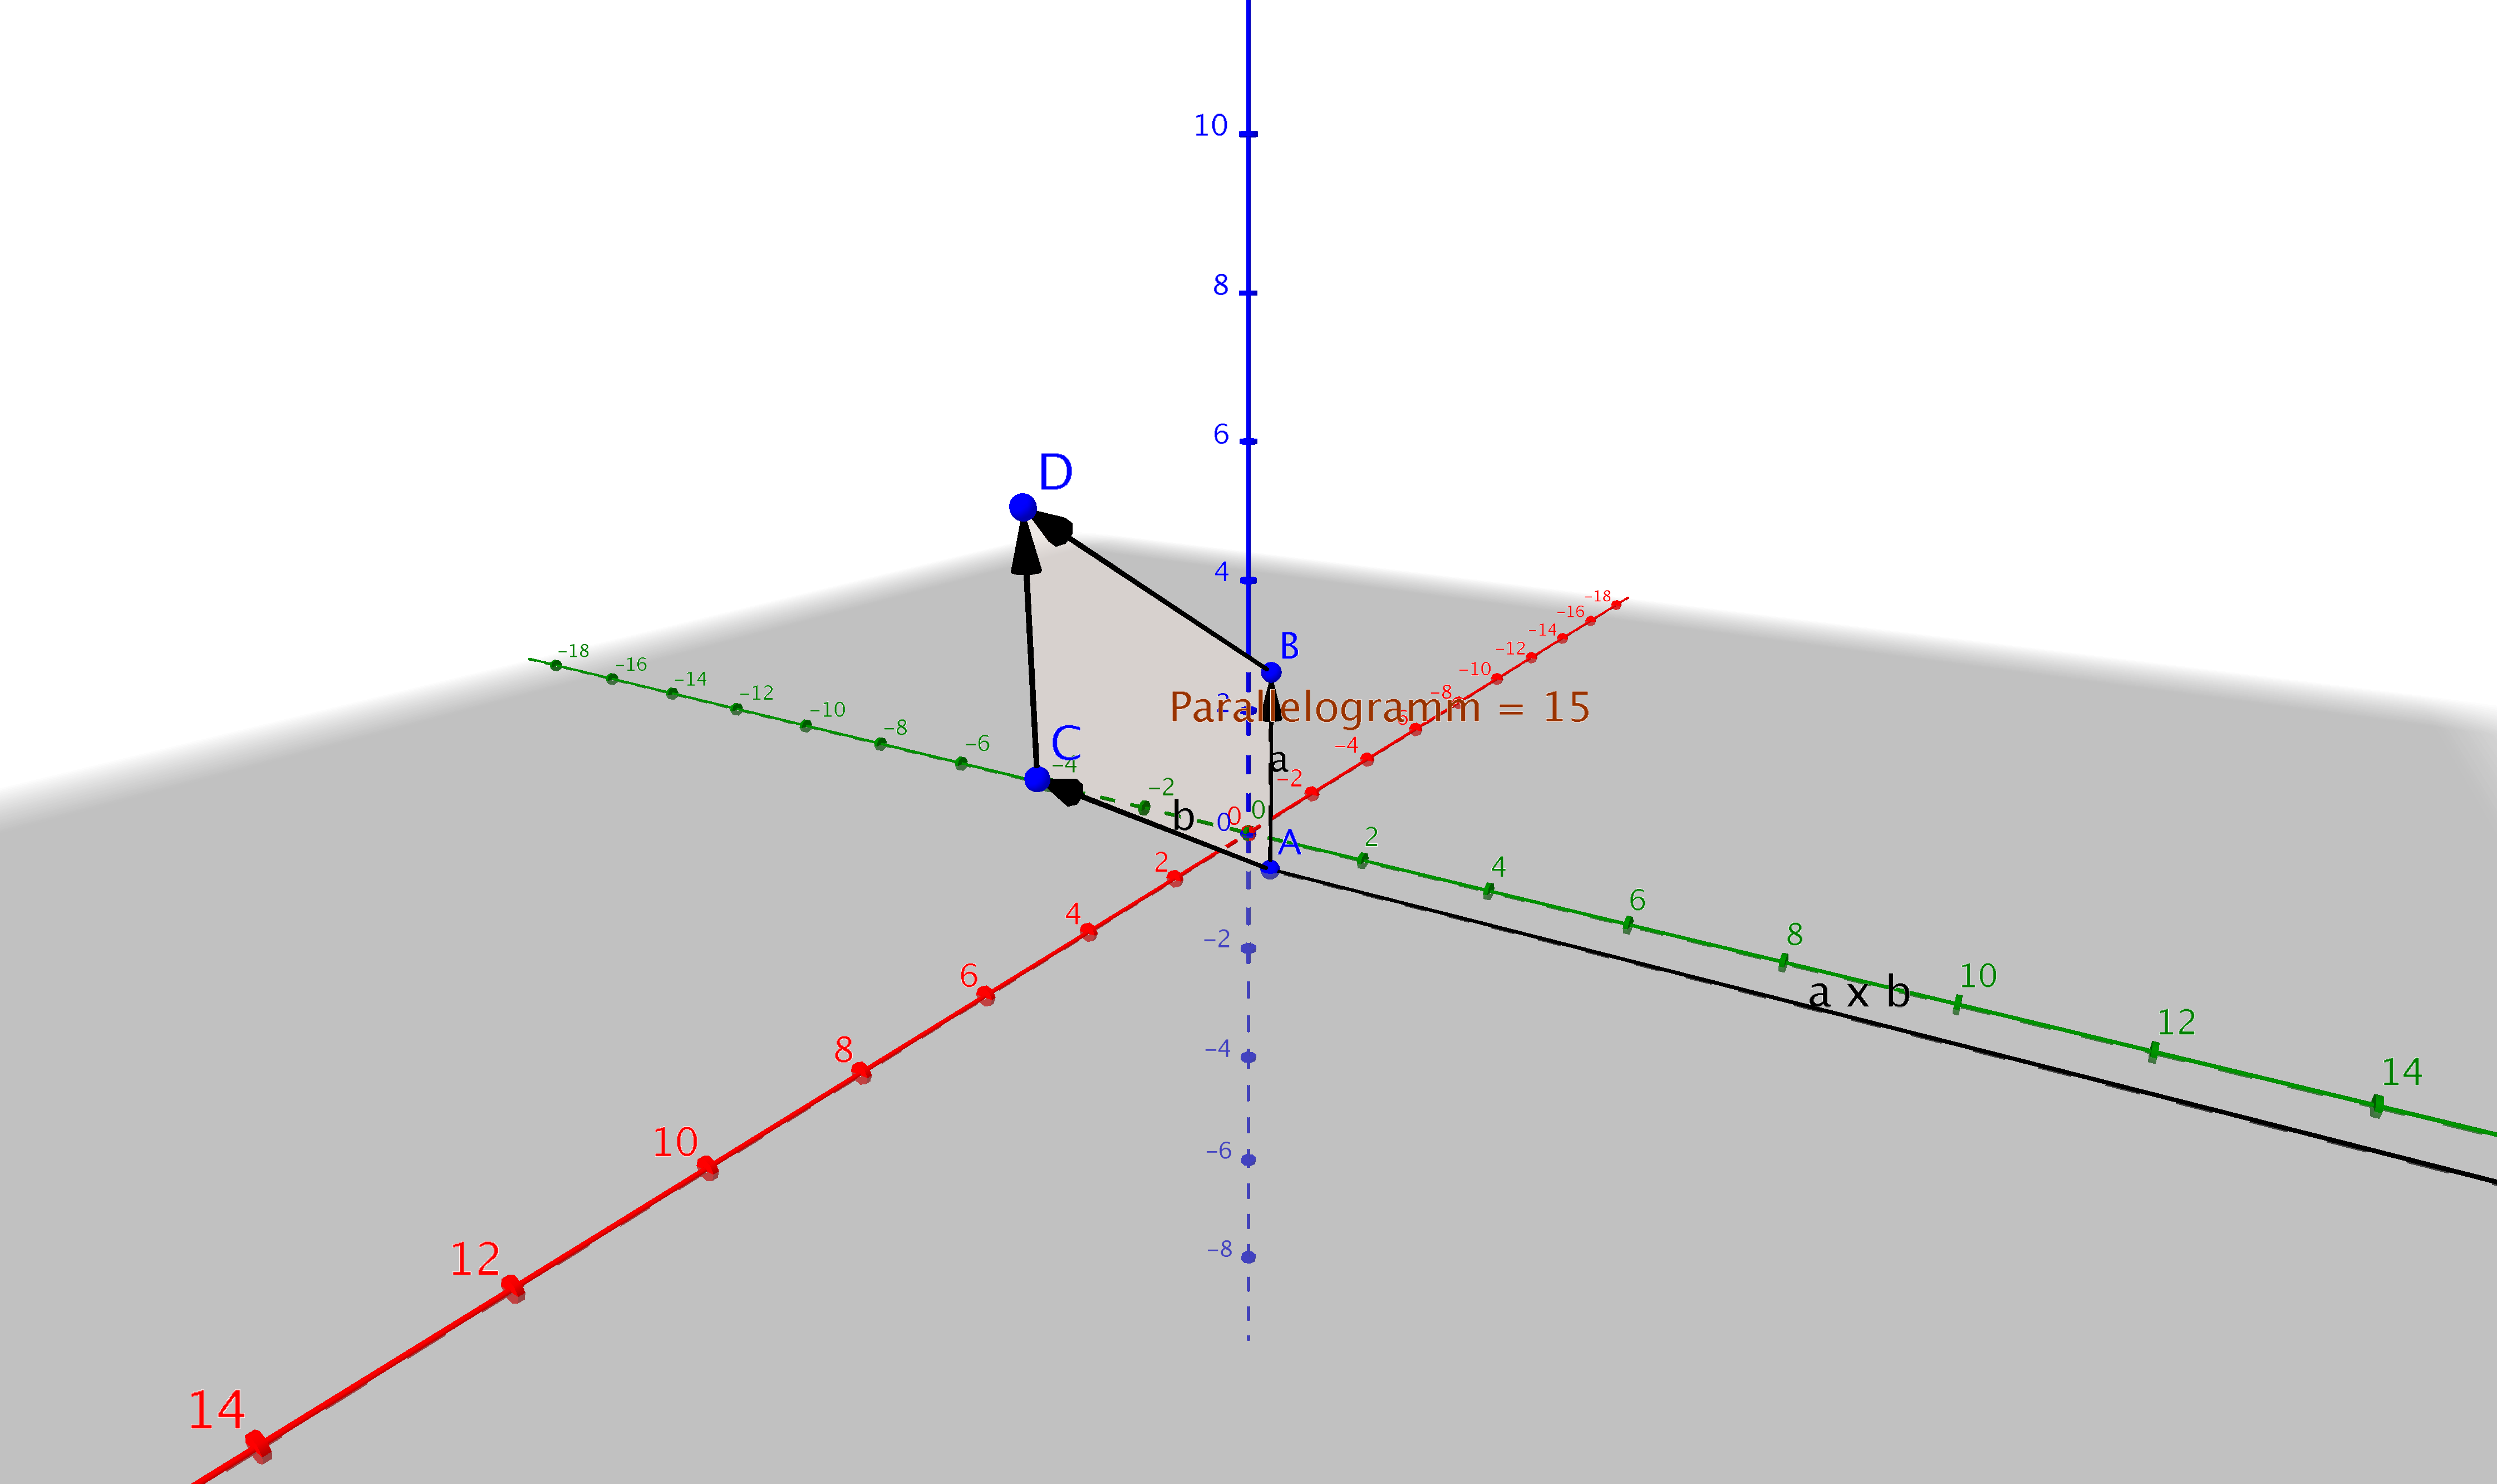
\includegraphics[width=10cm]{parallelogramm.png}
\end{frame}

\begin{frame}{Kreuzprodukt - Drehmoment}
	Greift eine Kraft $\vv{F}$ am Rand einer drehbar  gelagerten Kreisscheibe mit dem Ortsvektor $\vv{r}$ an, so wirkt auf die Scheibe das Drehmoment
	\[
		\vv{M} = \vv{r} \times \vv{F}
	\]
	mit
	\[
		\| \vv{M} \| = \| \vv{r}\| \|\vv{F}\| \sin \alpha
	\]
\definecolor{qqwuqq}{rgb}{0.,0.39215686274509803,0.}
\definecolor{uuuuuu}{rgb}{0.26666666666666666,0.26666666666666666,0.26666666666666666}
\definecolor{xdxdff}{rgb}{0.49019607843137253,0.49019607843137253,1.}
\definecolor{qqqqff}{rgb}{0.,0.,1.}
\begin{tikzpicture}[line cap=round,line join=round,>=triangle 45,x=0.9cm,y=0.9cm]
\draw[->,color=black] (-1.6177777777777769,0.) -- (8.853333333333339,0.);
\foreach \x in {-1.5,-1.,-0.5,0.5,1.,1.5,2.,2.5,3.,3.5,4.,4.5,5.,5.5,6.,6.5,7.,7.5,8.,8.5}
\draw[shift={(\x,0)},color=black] (0pt,2pt) -- (0pt,-2pt) node[below] {\footnotesize $\x$};
\draw[->,color=black] (0.,-0.18666666666666967) -- (0.,6.035555555555551);
\foreach \y in {,0.5,1.,1.5,2.,2.5,3.,3.5,4.,4.5,5.,5.5,6.}
\draw[shift={(0,\y)},color=black] (2pt,0pt) -- (-2pt,0pt) node[left] {\footnotesize $\y$};
\draw[color=black] (0pt,-10pt) node[right] {\footnotesize $0$};
\clip(-1.6177777777777769,-0.18666666666666967) rectangle (8.853333333333339,6.035555555555551);
\draw [shift={(3.7680568414275446,4.4236284792602305)},color=green,fill=green,fill opacity=0.1] (0,0) -- (-36.111057521575496:0.5666666666666668) arc (-36.111057521575496:8.623241639417227:0.5666666666666668) -- cycle;
\draw(2.,2.) circle (2.7cm);
\draw [->] (2.,2.) -- (3.7680568414275446,4.4236284792602305);
\draw [->] (3.7680568414275446,4.4236284792602305) -- (8.36,5.12);
\draw [->] (3.7680568414275446,4.4236284792602305) -- (6.43349336850494,2.479170684916884);
\draw [dash pattern=on 2pt off 2pt] (8.36,5.12)-- (6.43349336850494,2.479170684916884);
\begin{scriptsize}
\draw [fill=qqqqff] (2.,2.) circle (1.5pt);
\draw[color=qqqqff] (2.062222222222225,2.124444444444441) node {$M$};
%\draw[color=black] (0.5244444444444462,4.44444444444444) node {$???$};
\draw [fill=xdxdff] (3.7680568414275446,4.4236284792602305) circle (1.5pt);
\draw[color=xdxdff] (3.8311111111111145,4.551111111111107) node {$P$};
\draw[color=black] (2.88,3.306666666666663) node {$r$};
\draw [fill=qqqqff] (8.36,5.12) circle (1.5pt);
\draw[color=qqqqff] (8.417777777777784,5.24444444444444) node {$A$};
\draw[color=black] (6.08,4.88) node {$F$};
\draw [fill=uuuuuu] (6.43349336850494,2.479170684916884) circle (1.5pt);
\draw[color=uuuuuu] (6.497777777777782,2.604444444444441) node {$B$};
\draw[color=black] (5.351111111111115,3.555555555555552) node {$\vv{F}^{\perp}_{\vv{r}}$};
\draw[color=qqwuqq] (4.8933333333333366,4.357777777777774) node {$\alpha = 44.73\textrm{\degre}$};
\end{scriptsize}
\end{tikzpicture}	
\end{frame}

\subsubsection{Spatprodukt}
\begin{frame}{Spatprodukt}
	Ein durch drei Vektoren $\vv{a}, \vv{b}, \vv{c} \in \mathbb{R}^3$ aufgespanntes Parallelotop/Spat hat das Volumen
	\[
		V = \left| \vv{a} \cdot \left( \vv{b} \times \vv{c} \right) \right|
	\]
	\begin{definition}
		Der Ausdruck
		\[
			\left< \vv{a}, \vv{b}, \vv{c} \right> := \vv{a} \cdot \left( \vv{b} \times \vv{c} \right)
		\]
		heißt \textbf{Spatprodukt} der Vektoren $\vv{a}, \vv{b}, \vv{c}$
	\end{definition}
\end{frame}

\begin{frame}{Spatprodukt - Geometrie}
	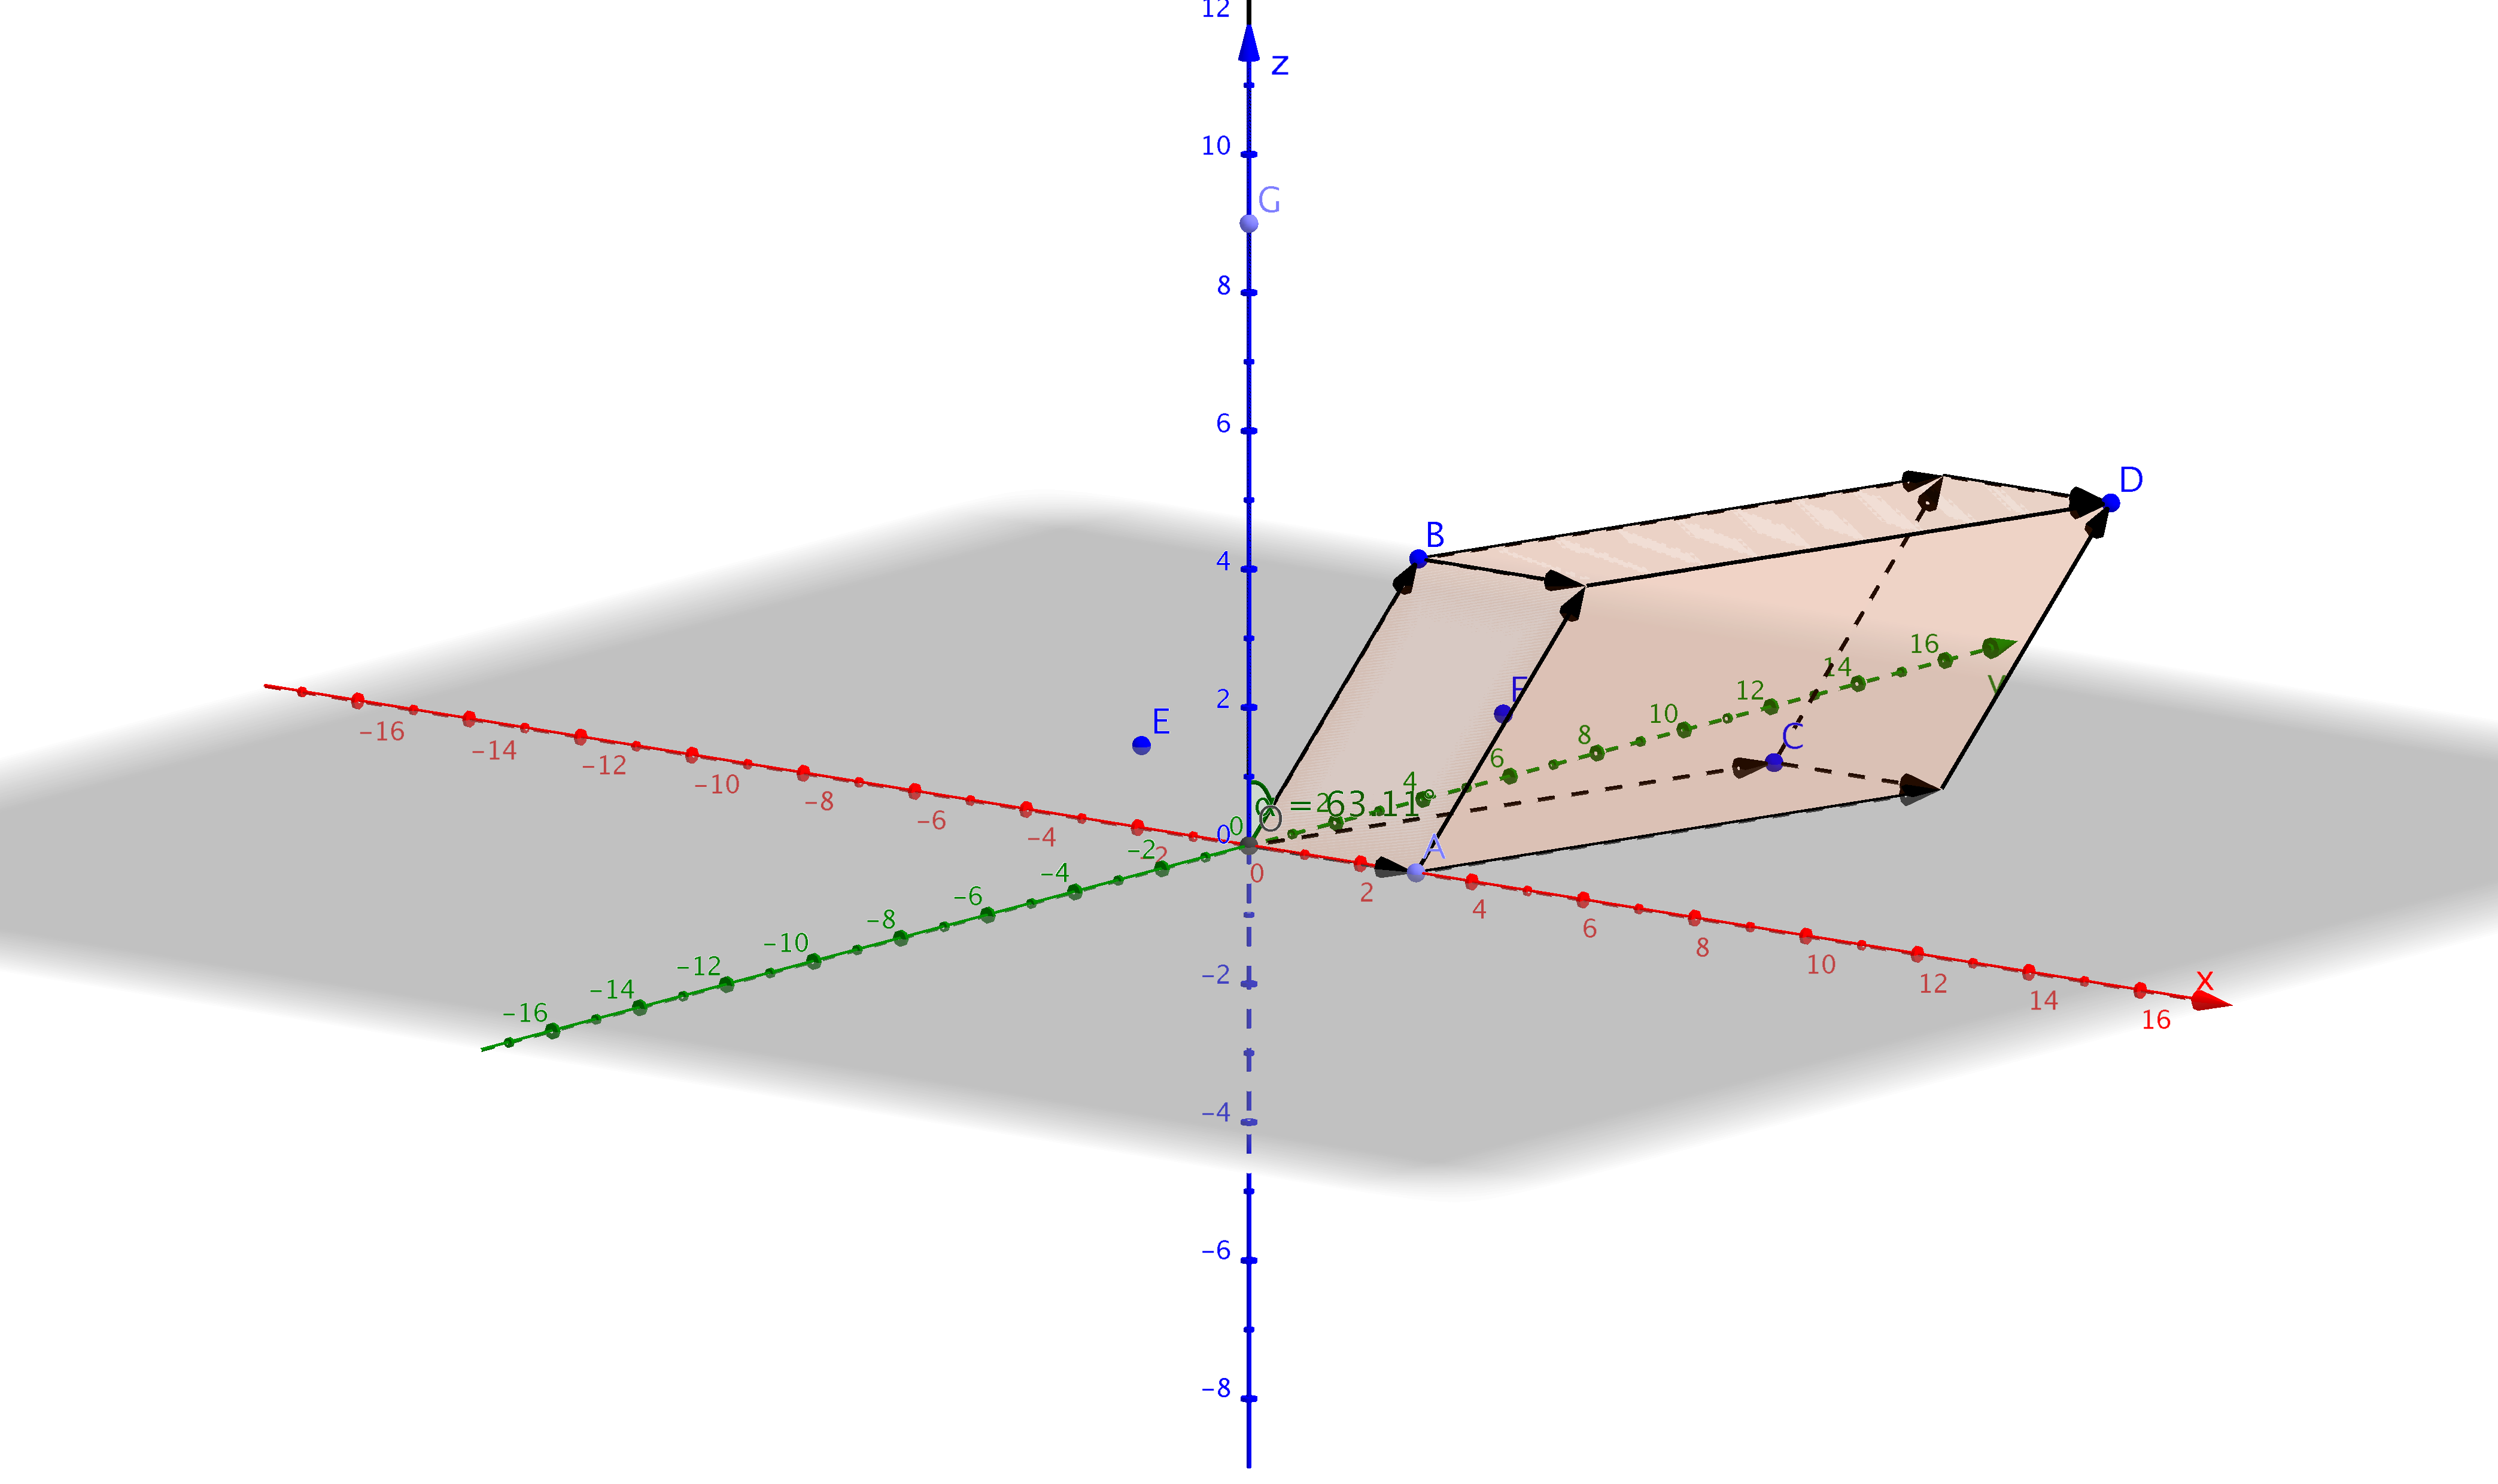
\includegraphics[width=10cm]{parallelotop.png}
	
	\href{/Users/stefan/sciebo/Mathematik/EigeneVorlesung/Folien/parallelotop.ggb}{Parallelotop Geogebra}
\end{frame}

\begin{frame}{Geraden - Parameterdarstellung}
	Eine Gerade ist durch die Angabe zweier Punkte auf ihr eindeutig bestimmt.
	
	Sind $A$ und $B$ zwei (verschiedene) Punkte einer Geraden und $\vv{a}$ und $\vv{b}$ die dazugehörigen Ortsvektoren,
	so kann man die Menge der Punkte der Geraden $g(A,B)$ durch $A$ und $B$ definieren als:
	\[
		g(A,B) := \left\{ \vv{y} \in \mathbb{R}^n \middle| \vv{y} = \vv{a} + \lambda \left( \vv{b} - \vv{a}\right), \lambda \in \mathbb{R}\right\}
	\]
	Diese Darstellung einer Geraden heißt \textbf{Parameterdarstellung der Geraden}. Der Parameter ist hier das $\lambda$.
\end{frame}

\subsection{Analytische Geometrie}
\subsubsection{Geraden}
\begin{frame}{Parameterdarstellung einer Gerade - Beispiel}
	Für die Punkte $A=\begin{pmatrix}
	3 \\ 4 \\ 1
	\end{pmatrix}$ und $B=\begin{pmatrix}
	2 \\ 4 \\ -1
	\end{pmatrix}$ ist
	\[
		g(A,B)  =  \left\{ \vv{y} \in \mathbb{R}^3 \middle| \vv{y} = \begin{pmatrix}
		3 \\ 4 \\ 1
		\end{pmatrix}
		 + \lambda \begin{pmatrix}
		 -1 \\ 0 \\ -2
		 \end{pmatrix}, \lambda \in \mathbb{R}\right\}
	\]
	Das ist z. B.
	\begin{itemize}
		\item für $\lambda = 0$ der Punkt $A$ mit dem Ortsvektor $\begin{pmatrix}
			3 \\ 4 \\ 1
		\end{pmatrix} $
		\item für $\lambda = 1$ der Punkt $B$ mit dem Ortsvektor $\begin{pmatrix}
			2 \\ 4 \\ -1
		\end{pmatrix}$
		\item und für $\lambda = 2$ der Punkt mit dem Ortsvektor $\begin{pmatrix}
			1 \\ 4 \\ -3
		\end{pmatrix}$
	\end{itemize}
\end{frame}

\begin{frame}{Parameterdarstellung einer Gerade}
	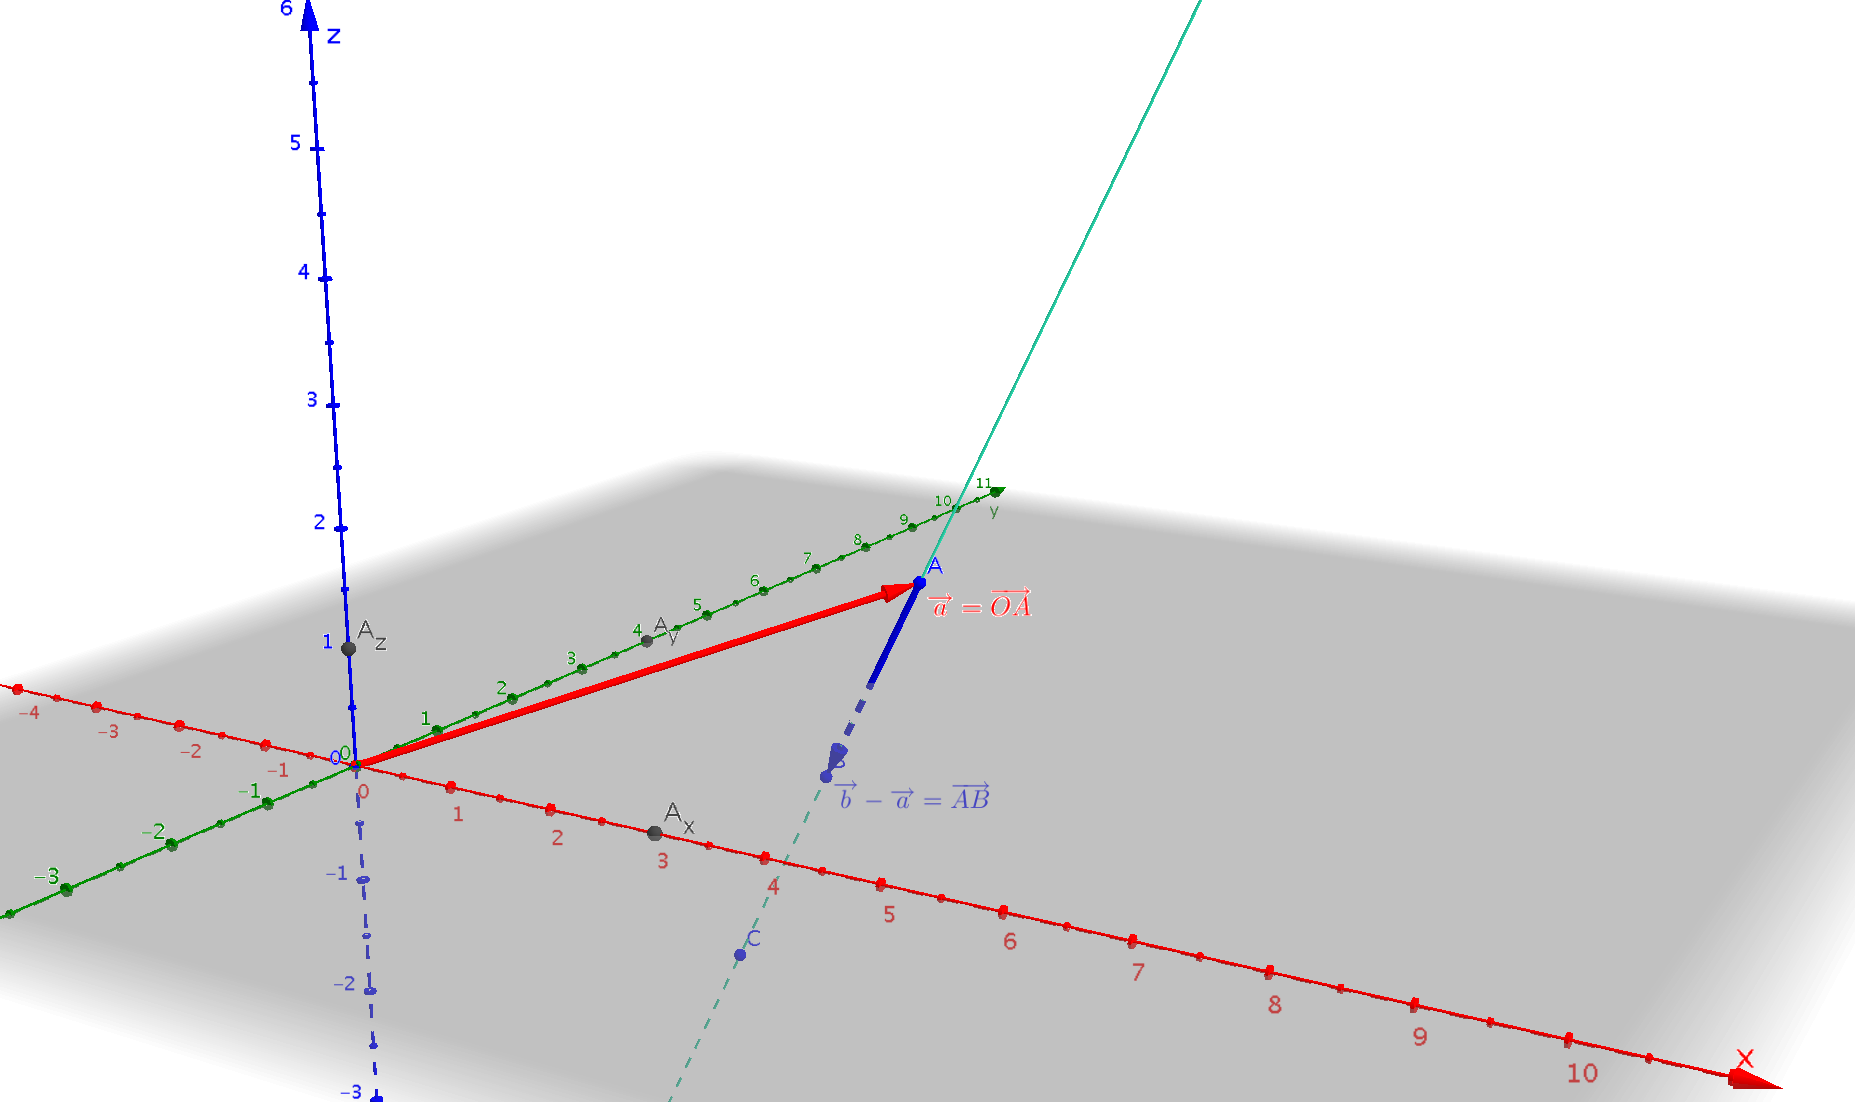
\includegraphics[width=10cm]{geradengleichung.png}
\end{frame}

\begin{frame}{Parameterdarstellung einer Geraden im $\mathbb{R}^2$}
	Eigentlich kennen Sie eine Gerade im $\mathbb{R}^2$ so:
	\[
		g = \left\{ \begin{pmatrix}
		x \\ y
		\end{pmatrix} \middle| y = m x + b \right\}
	\]
	und $b$ ist der y-Achsenabschnitt und $m$ die Steigung der Geraden.
	Das sieht dann zum Beispiel so aus:
	\definecolor{qqqqff}{rgb}{0.,0.,1.}
	\definecolor{xdxdff}{rgb}{0.49019607843137253,0.49019607843137253,1.}
	\begin{tikzpicture}[line cap=round,line join=round,>=triangle 45,x=0.6cm,y=0.6cm]
	\draw[->,color=black] (-2.713333333333333,0.) -- (12.99333333333334,0.);
	\foreach \x in {-2.,-1.,1.,2.,3.,4.,5.,6.,7.,8.,9.,10.,11.,12.}
	\draw[shift={(\x,0)},color=black] (0pt,2pt) -- (0pt,-2pt) node[below] {\footnotesize $\x$};
	\draw[->,color=black] (0.,-5.233333333333338) -- (0.,4.1);
	\foreach \y in {-5.,-4.,-3.,-2.,-1.,1.,2.,3.,4.}
	\draw[shift={(0,\y)},color=black] (2pt,0pt) -- (-2pt,0pt) node[left] {\footnotesize $\y$};
	\draw[color=black] (0pt,-10pt) node[right] {\footnotesize $0$};
	\clip(-2.713333333333333,-5.233333333333338) rectangle (12.99333333333334,4.1);
	\draw [domain=-2.713333333333333:12.99333333333334] plot(\x,{(-8.--2.*\x)/4.});
	\draw [->] (0.,-2.) -- (4.,-2.);
	\draw [->] (4.,-2.) -- (4.,0.);
	\draw (1.4066666666666687,-1.80666666666667) node[anchor=north west] {$\Delta x \, = \,4$};
	\draw (4.0466666666666695,-0.74) node[anchor=north west] {$\Delta y \, = \,2$};
	\draw (6.62,-2.24) node[anchor=north west] {$b \, = \,-2$};
	\draw (6.56666666666667,-1.36666666666667) node[anchor=north west] {$m \, = \, \frac{\Delta y}{\Delta x} \, = \,\frac{1}{2}$};
	\begin{scriptsize}
	\draw [fill=xdxdff] (0.,-2.) circle (1.5pt);
	\draw[color=xdxdff] (0.08666666666666821,-1.80666666666667) node {$A$};
	\draw [fill=qqqqff] (4.,0.) circle (1.5pt);
	\draw[color=qqqqff] (4.08666666666667,0.19333333333333036) node {$B$};
	\draw[color=black] (7.046666666666666,3.06) node {$g: y = \frac{1}{2}x - 2$};
	\end{scriptsize}
	\end{tikzpicture}
\end{frame}


\begin{frame}{Parameterdarstellung Gerade im $\mathbb{R}^2$}
	Auf dieser Geraden $y=mx+b$ liegen z.B. die Punkte
	\[
	A = \begin{pmatrix} 0 \\ b \end{pmatrix}
	\mbox{ und }
	B = \begin{pmatrix} -\frac{b}{m}\\ 0 \end{pmatrix}
	\mbox{ oder }
	D = \begin{pmatrix} 1 \\ m + b \end{pmatrix}
	\]
	\definecolor{uuuuuu}{rgb}{0.26666666666666666,0.26666666666666666,0.26666666666666666}
	\definecolor{ffxfqq}{rgb}{1.,0.4980392156862745,0.}
	\definecolor{qqqqff}{rgb}{0.,0.,1.}
	\definecolor{xdxdff}{rgb}{0.49019607843137253,0.49019607843137253,1.}
	\begin{tikzpicture}[line cap=round,line join=round,>=triangle 45,x=0.6cm,y=0.6cm]
	\draw[->,color=black] (-2.7133333333333325,0.) -- (12.99333333333334,0.);
	\foreach \x in {-2.,-1.,1.,2.,3.,4.,5.,6.,7.,8.,9.,10.,11.,12.}
	\draw[shift={(\x,0)},color=black] (0pt,2pt) -- (0pt,-2pt) node[below] {\footnotesize $\x$};
	\draw[->,color=black] (0.,-5.233333333333337) -- (0.,4.1);
	\foreach \y in {-5.,-4.,-3.,-2.,-1.,1.,2.,3.,4.}
	\draw[shift={(0,\y)},color=black] (2pt,0pt) -- (-2pt,0pt) node[left] {\footnotesize $\y$};
	\draw[color=black] (0pt,-10pt) node[right] {\footnotesize $0$};
	\clip(-2.7133333333333325,-5.233333333333337) rectangle (12.99333333333334,4.1);
	\draw [domain=-2.7133333333333325:12.99333333333334] plot(\x,{(-8.--2.*\x)/4.});
	\draw [->,line width=2.pt,color=ffxfqq] (0.,0.) -- (0.,-2.);
	\draw [->] (0.,-2.) -- (4.,-2.);
	\draw [->] (4.,-2.) -- (4.,0.);
	\draw (1.3933333333333358,-1.80666666666667) node[anchor=north west] {$\Delta x \, = \,4$};
	\draw (4.0466666666666695,-0.74) node[anchor=north west] {$\Delta y \, = \,2$};
	\draw (6.62,-2.24) node[anchor=north west] {$b \, = \,-2$};
	\draw (6.553333333333337,-1.36666666666667) node[anchor=north west] {$m \, = \frac{\Delta y}{\Delta x} \, = \,\frac{1}{2}$};
	\draw [->] (0.,0.) -- (1.,-1.5);
	\begin{scriptsize}
	\draw [fill=xdxdff] (0.,-2.) circle (1.5pt);
	\draw[color=xdxdff] (0.08666666666666858,-1.80666666666667) node {$A$};
	\draw [fill=qqqqff] (4.,0.) circle (1.5pt);
	\draw[color=qqqqff] (4.08666666666667,0.19333333333333036) node {$B$};
	\draw[color=black] (7.046666666666666,3.06) node {$g: y = \frac{1}{2}x - 2$};
	\draw [fill=uuuuuu] (1.,-1.5) circle (1.5pt);
	\draw[color=uuuuuu] (1.086666666666669,-1.3133333333333366) node {$D$};
	\end{scriptsize}
	\end{tikzpicture}
\end{frame}

\begin{frame}{Zusammenhang zwischen Geradengleichungen}
	Für eine Gerade $g$ mit der Funktionsgleichung
	\[
	g: y = m x + b \qquad x \in \mathbb{R}
	\]
	gilt also zum Beispiel:
	\[
	g = \left\{ \vv{a} = \begin{pmatrix}x \\ y\end{pmatrix} \in \mathbb{R}^2 \middle| \vv{a} = \begin{pmatrix}
	0 \\ b
	\end{pmatrix} + \lambda \begin{pmatrix}
	-\frac{b}{m} \\ -b
	\end{pmatrix}, \lambda \in \mathbb{R} \right\}
	\]
	Umgekehrt gilt für eine Gerade
	\[
	g = \left\{ \begin{pmatrix}x \\ y\end{pmatrix} \in \mathbb{R}^2 \middle| \begin{pmatrix}
	x \\ y
	\end{pmatrix} = \vv{a}  + \lambda \vv{b}, \lambda \in \mathbb{R} \right\}
	\]
	wegen $\lambda = \frac{x-a_x}{b_x}$ \footnote{also auch nur, wenn $b_x \neq 0$ ist} die Funktionsdarstellung
	\[
	g: y = a_y + \frac{b_y}{b_x} \left( x - a_x \right) = \frac{b_y}{b_x} x + \left(a_y - \frac{b_y}{b_x} a_x\right)
	\]
\end{frame}


\begin{frame}{Anwendungsbeispiel - Diagonalen im Parallelogramm}
	\begin{theorem}
		In einem Parallelogramm halbieren sich die Diagonalen.
	\end{theorem}
	\definecolor{uuuuuu}{rgb}{0.26666666666666666,0.26666666666666666,0.26666666666666666}
	\definecolor{qqqqff}{rgb}{0.,0.,1.}
	\begin{tikzpicture}[line cap=round,line join=round,>=triangle 45,x=1.0cm,y=1.0cm]
	\draw[->,color=black] (-0.31333333333333263,0.) -- (10.15777777777778,0.);
	\foreach \x in {,0.5,1.,1.5,2.,2.5,3.,3.5,4.,4.5,5.,5.5,6.,6.5,7.,7.5,8.,8.5,9.,9.5,10.}
	\draw[shift={(\x,0)},color=black] (0pt,2pt) -- (0pt,-2pt) node[below] {\footnotesize $\x$};
	\draw[->,color=black] (0.,-0.19333333333333416) -- (0.,6.028888888888882);
	\foreach \y in {,0.5,1.,1.5,2.,2.5,3.,3.5,4.,4.5,5.,5.5,6.}
	\draw[shift={(0,\y)},color=black] (2pt,0pt) -- (-2pt,0pt) node[left] {\footnotesize $\y$};
	\draw[color=black] (0pt,-10pt) node[right] {\footnotesize $0$};
	\clip(-0.31333333333333263,-0.19333333333333416) rectangle (10.15777777777778,6.028888888888882);
	\draw [->] (1.,2.) -- (6.,2.);
	\draw [->] (1.,2.) -- (2.,5.);
	\draw [->] (6.,2.) -- (7.,5.);
	\draw [->] (2.,5.) -- (7.,5.);
	\draw [->] (1.,2.) -- (7.,5.);
	\draw [->] (2.,5.) -- (6.,2.);
	\draw (2.264444444444446,3.077777777777774) node[anchor=north west] {$\vv{a}+\vv{b}$};
	\draw (2.8755555555555574,4.688888888888884) node[anchor=north west] {$\vv{a}- \vv{b}$};
	\draw [domain=-0.31333333333333263:10.15777777777778] plot(\x,{(--9.--3.*\x)/6.});
	\draw [domain=-0.31333333333333263:10.15777777777778] plot(\x,{(--26.-3.*\x)/4.});
	\begin{scriptsize}
	\draw [fill=qqqqff] (1.,2.) circle (1.5pt);
	\draw[color=qqqqff] (1.0644444444444454,2.126666666666664) node {$A$};
	\draw [fill=qqqqff] (2.,5.) circle (1.5pt);
	\draw[color=qqqqff] (2.06,5.122222222222216) node {$D$};
	\draw [fill=qqqqff] (6.,2.) circle (1.5pt);
	\draw[color=qqqqff] (6.06,2.126666666666664) node {$B$};
	\draw[color=black] (3.5177777777777797,2.108888888888886) node {$\vv{a}$};
	\draw[color=black] (1.4911111111111122,3.58444444444444) node {$\vv{b}$};
	\draw [fill=qqqqff] (7.,5.) circle (1.5pt);
	\draw[color=qqqqff] (7.0644444444444465,5.122222222222216) node {$C$};
	\draw [fill=qqqqff] (7.,5.) circle (1.5pt);
%	\draw[color=qqqqff] (7.091111111111114,5.122222222222216) node {$D'$};
	\draw [fill=uuuuuu] (4.,3.5) circle (1.5pt);
	\draw[color=uuuuuu] (4.06,3.8288888888888846) node {$S_d$};
	\end{scriptsize}
	\end{tikzpicture}
	
\end{frame}

\begin{frame}{Beweis: Diagonalen im Parallelogramm halbieren sich}
		\begin{scriptsize}

		\textbf{Denn:} Das Parallelogramm werde aufgespannt von den Vektoren $\vv{a}$ und $\vv{b}$.
		Der Schnittpunkt der Diagonalen ist der Schnittpunkt der beiden Geraden
		\[
		\vv{OA} + \vv{b} + \lambda \left(\vv{a} - \vv{b}\right) \mbox{ und } 	\vv{OA} + \mu \left(\vv{a} + \vv{b}\right)
		\]
		Der Schnittpunkt der beiden Geraden muß  beide Gleichungen erfüllen, also
		\[
		\cancel{\vv{OA}} + \vv{b} + \lambda \left(\vv{a} - \vv{b}\right) =	\cancel{\vv{OA}} + \mu \left(\vv{a} + \vv{b}\right)
		\]
		oder nach Sortierung der Terme nach $\vv{a}$ und $\vv{b}$ \[
		\left(1-\lambda-\mu\right) \vv{b} = \left(\mu - \lambda \right) \vv{a}
		\]
		Wäre nun $\mu - \lambda \neq 0$, so könnte man beide Seite durch $\mu - \lambda$ dividieren und erhielte:
		\[
		\frac{1 - \lambda - \mu}{\mu - \lambda} \vv{b} = \vv{a}
		\]
		Dann aber wären $\vv{a}$ und $\vv{b}$ parallel und könnten kein Parallelogramm aufspannen.
		
		Also ist $\mu = \lambda$ und genauso auch $1 - \mu - \lambda = 0$, also
		\[
		\lambda = \mu = \frac{1}{2}
		\]
		\end{scriptsize}
\end{frame}

\subsubsection{Ebenen}

\begin{frame}{Ebenen - Parameterdarstellung}
	Eine Ebene ist durch die Angabe dreier Punkte auf ihr eindeutig bestimmt.
	
	Sind $A$, $B$ und $C$ drei (verschiedene) Punkte und $\vv{a}$, $\vv{b}$ und $\vv{c}$ die dazugehörigen Ortsvektoren, so kann man die Menge der Punkte der Ebene $E(A,B,C)$ durch die Punkte $A$, $B$ und $C$ definieren als:
	\[
		E(A,B,C) := \left\{ \vv{y} \in \mathbb{R}^n \middle| \vv{y} = \vv{a} + \lambda \left(\vv{b} - \vv{a} \right) + \mu \left(\vv{c} - \vv{a} \right); \lambda, \mu \in \mathbb{R} \right\}
	\]
	Diese Darstellung einer Ebene heißt \textbf{Parameterdarstellung der Ebene}. Die Parameter sind hier $\lambda$ und $\mu$.
\end{frame}

\begin{frame}{Parameterdarstellung einer Ebene - Beispiel}
	
	{\footnotesize Für die Punkte $A=\begin{pmatrix}1\\2\\3\end{pmatrix}$, $B=\begin{pmatrix}3\\-1\\3\end{pmatrix}$ und $C=\begin{pmatrix}4\\-3\\0\end{pmatrix}$ ist
	\[
	E(A,B,C):= \left\{ \vv{y} \in \mathbb{R} \middle| \vv{y} = \begin{pmatrix}
	1\\2\\3
	\end{pmatrix} + \lambda \begin{pmatrix}
	2\\-3\\0
	\end{pmatrix} + \mu \begin{pmatrix}
	3\\-5\\-3
	\end{pmatrix} \right\}
	\]
	Dabei ist z.B.
	\begin{itemize}
	\item für $\lambda = 0$ und $\mu = 0$ der Punkt $A$ mit dem Ortsvektor $\begin{pmatrix}1\\2\\3\end{pmatrix}$
	\item für $\lambda = 1$ und $\mu = 0$ der Punkt $B$ mit dem Ortsvektor $\begin{pmatrix}3\\-1\\3\end{pmatrix}$
	\item für $\lambda = 0$ und $\mu = 1$ der Punkt $C$ mit dem Ortsvektor $\begin{pmatrix}4\\-3\\0\end{pmatrix}$
	\item für $\lambda = 1$ und $\mu = 1$ der Punkt $D$ mit dem Ortsvektor $\begin{pmatrix}6\\-6\\0\end{pmatrix}$
	\end{itemize}}
\end{frame}

\begin{frame}{Parameterdarstellung einer Ebene - Grafik}
	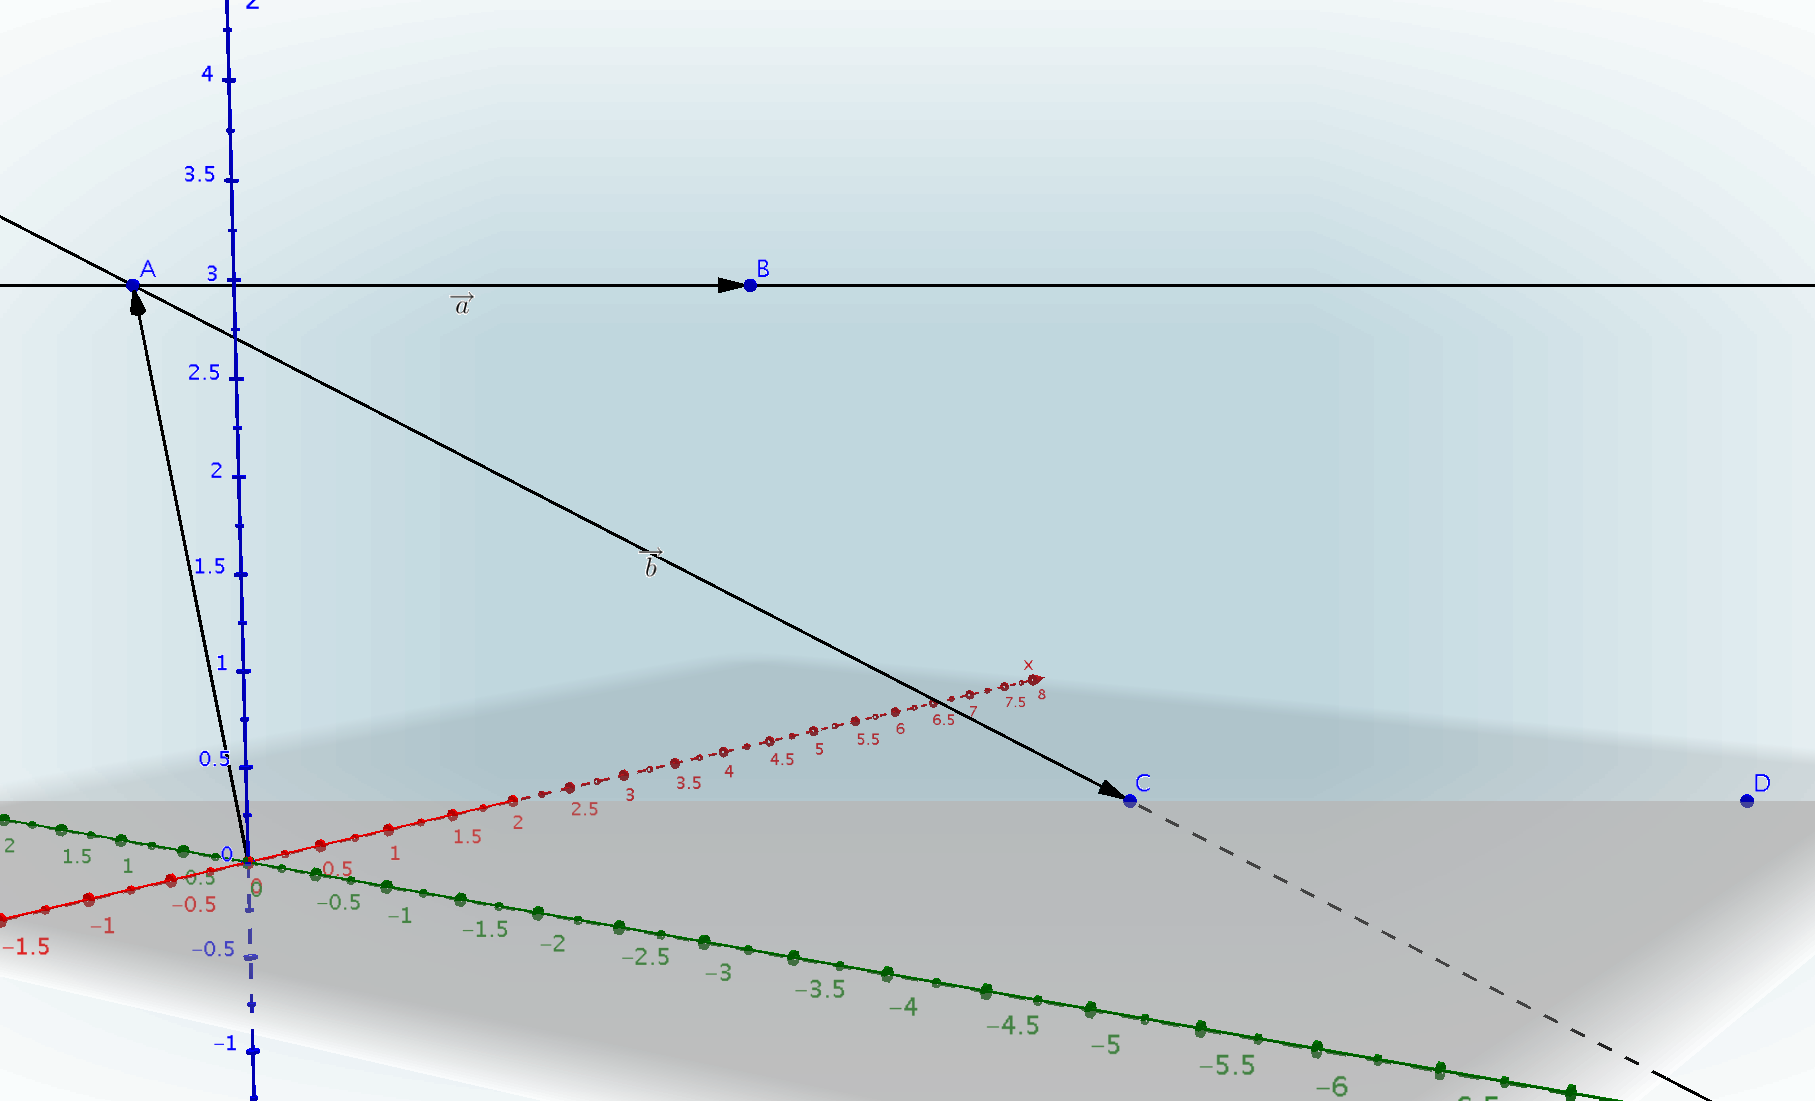
\includegraphics[width=10cm,height=8cm]{ebenengleichung.png}
\end{frame}

\begin{frame}{Normalenform einer Ebene}
	Man kann eine Ebene algebraisch auch anders darstellen.
	
	Diese Darstellung beruht auf der Idee, daß  es einen Vektor $\vv{n}$ gibt, der auf der Ebene senkrecht steht, d.h. der Vektor steht senkrecht auf allen in der Ebene liegenden Vektoren, also insbesondere auch
	\[ \vv{n} \perp \vv{u} = \vv{n} \perp (\vv{b} - \vv{a}) \qquad\mbox{und}\qquad
	\vv{n} \perp \vv{v} = \vv{n} \perp (\vv{c} - \vv{a})\]
	Es gibt aber einen speziellen Vektor, der sowohl auf $\vv{u}$ als auch auf $\vv{v}$ senkrecht steht:
	\[
		\vv{n} = \vv{u} \times \vv{v}
	\]
	Für alle Punkte der Ebene gilt damit
	\begin{framed}
		\begin{center}
		\textbf{Normalenform einer Ebene}\end{center}
	\[
	E(A,B,C) = \left\{ \vv{y} \in \mathbb{R}^3 \middle| \vv{n} \cdot \left( \vv{y} - \vv{a}\right) = 0 \right\}
	\]
	\end{framed}
\end{frame}

\begin{frame}{Umrechnung der Parameterform in Normalform}
	Um von einer Parameterdarstellung
	\[
			E = \left\{ \vv{y} \in \mathbb{R}^n \middle| \vv{y} = \vv{a} + \lambda \vv{u}  + \mu \vv{v}; \lambda, \mu \in \mathbb{R} \right\}
	\]
	in die Normalenform umzurechnen, geht man wie folgt vor:
	\begin{enumerate}
		\item Berechnung des Normalenvektors
		\[
		\vv{n} = \begin{pmatrix}
		n_1 \\ n_2 \\ n_3
		\end{pmatrix} = \vv{u} \times \vv{v}
		\]
		\item Berechnung des Skalarproduktes
		\[
		c = \vv{n} \cdot \vv{a} = n_1 a_1 + n_2 a_2 + n_3 a_3
		\]
		\item Die Normalenform ist dann
		\[
		\vv{n} \cdot \vv{y} = \vv{n} \cdot \vv{a} = 0 \Leftrightarrow n_1 y_1 + n_2 y_2 + n_3 y_3 = c
		\]
	\end{enumerate}	
\end{frame}

\begin{frame}{Umrechnung Normalform in Parameterform}
	Um von der Normalform
	\[
	E = \vv{n} \cdot \vv{y} = n_1 y_1 + n_2 y_2 + n_3 y_3 = c
	\]
	in die Parameterdarstellung umzurechnen geht man wie folgt vor:
	\begin{enumerate}
		\item Berechnung dreier Punkte der Ebene mittels der Normalform, z.B.
		\[
		A = \begin{pmatrix}
		\frac{c}{n_1} \\0 \\0
		\end{pmatrix} \qquad B = \begin{pmatrix}
		0\\ \frac{c}{n_2} \\ 0
		\end{pmatrix} \qquad C = \begin{pmatrix}
		0\\ 0 \\ \frac{c}{n_3}
		\end{pmatrix}
		\]
		\item Berechnung eines Ortsvektors und der beiden Richtungsvektoren
		\[
		\vv{a} := \vv{OA}\]
		und
		\[
		\vv{u} := \vv{b} - \vv{a} := \vv{OB} - \vv{a} \qquad \mbox{und}\qquad \vv{v} := \vv{c} - \vv{a} := \vv{OC} - \vv{a}
		\]
	\end{enumerate}
\end{frame}

\begin{frame}{Beispiel Normalform einer Ebene}
	Die Ebene aus dem vorherigen Beispiel
		\[
		E(A,B,C):= \left\{ \vv{y} \in \mathbb{R} \middle| \vv{y} = \begin{pmatrix}
		1\\2\\3
		\end{pmatrix} + \lambda \begin{pmatrix}
		2\\-3\\0
		\end{pmatrix} + \mu \begin{pmatrix}
		3\\-5\\-3
		\end{pmatrix} \right\}
		\]
	hat die Normalform	
	\begin{framed}
	\[
	9 y_1 + 6 y_2 - y_3 = 18
	\]
	\end{framed}
	{\footnotesize
	denn
	\[\vv{n} =
	\begin{pmatrix}
	2\\-3\\0
	\end{pmatrix} \times \begin{pmatrix}
	3\\-5\\-3
	\end{pmatrix} = \begin{pmatrix}
	(-3) \cdot (-3) - 0 \cdot 5 \\ 0 \cdot 3 - 2 \cdot (-3) \\ 2 \cdot (-5) - (-3) \cdot 3
	\end{pmatrix} = \begin{pmatrix}
	9 \\ 6 \\ -1
	\end{pmatrix}
	\]
	und
	\[
	\vv{n} \cdot \vv{a} = \begin{pmatrix}
	9 \\ 6 \\ -1
	\end{pmatrix} \cdot \begin{pmatrix}
	1\\2\\3
	\end{pmatrix} = 9\cdot 1 + 6 \cdot 2 + (-1)\cdot 3= 9 + 12 -3 = 18
	\] }
\end{frame}

\begin{frame}{Abstand Punkt-Ebene}
	Man kann mit Hilfe der Normalform einer Ebene den Abstand eines beliebigen Punktes zu dieser Ebene berechnen:
	\begin{framed}
	\begin{center}
		Abstandsformel
	\end{center}
	Der Abstand $d(P,E)$ eines Punktes $P$ mit dem Ortsvektor $\vv{p}$ zur Ebene $E : \vv{n} \cdot \left( \vv{y}  - \vv{a} \right) = 0$ ist
	\[
	d(P,E) = \frac{\vv{n} \cdot \left( \vv{p} - \vv{a} \right)}{\| \vv{n} \|} = \frac{\vv{n} \cdot \vv{p}}{\| \vv{n} \|} - \frac{\vv{n} \cdot \vv{a}}{\| \vv{n} \|}
	\]
	\end{framed}
	Man muß  also die Normalform nehmen und noch durch die Länge des Normalenvektors teilen.
\end{frame}

\subsection{Lineare Gleichungssysteme und Matrizen}
\subsubsection{Lineare Gleichungssysteme}

\begin{frame}{Lineare Algebra - Systeme linearer Funktionen und Gleichungen}

\begin{definition}
	
	Ein System von m linearen Gleichungen mit n Unbekannten der Form
\begin{align*}
a_{11} x_{1} + a_{12} x_{2} + a_{13} x_{3} + \ldots + a_{1n} x_{n}  & =   b_{1} \\
a_{21} x_{1} + a_{22} x_{2} + a_{23} x_{3} + \ldots + a_{2n} x_{n}  & =   b_{2} \\
a_{31} x_{1} + a_{32} x_{2} + a_{33} x_{3} + \ldots + a_{3n} x_{n}  & =   b_{3} \\
\vdots \qquad &  \\
a_{m1} x_{1} + a_{m2} x_{2} + a_{m3} x_{3} + \ldots + a_{mn} x_{n}  & =   b_{m}
\end{align*}
heißt \textbf{lineares Gleichungssystem}.
\end{definition}
\begin{bemerkung}
	Hierbei sind $a_{11}$, $a_{12}, \ldots , a_{mn}$ und $b_1 , \ldots , b_m$ vorgegebene reelle Zahlen, auch \textbf{Koeffizienten} genannt. Gesucht ist die Menge der $x_1$, $x_2, \ldots , x_n$ (\textbf{Lösung des Gleichungssystems}), die das Gleichungssystem erfüllen.
\end{bemerkung}
\end{frame}

\begin{frame}{Beispiele linearer Gleichungssysteme}
	\begin{example}
		Das lineare Gleichungssystem
		\begin{align*}
		a_{11} x + a_{12} y & = b_1 \\
		a_{21} x + a_{22} y & = b_2
		\end{align*}
		besteht geometrisch aus zwei Geradengleichungen im $\mathbb{R}^{2}_{(x,y)}$. Die Lösungsmenge dieses Gleichungssystems besteht aus all den Punkten, die auf beiden Geraden liegen, also gilt entweder
		\begin{itemize}
			\item die Lösungsmenge besteht genau aus dem Schnittpunkt der beiden Geraden oder
			\item die Lösungsmenge besteht aus allen Punkten der Geraden, weil beide Gleichungen vielleicht dieselbe Gerade beschreiben oder
			\item die Lösungsmenge ist leer, weil die Geraden parallel sind und es daher keine gemeinsamen Punkte gibt.
		\end{itemize}
			
	\end{example}
\end{frame}

\begin{frame}{Beispiele linearer Gleichungssysteme - Genau eine Lösung}
	\begin{example}
		Das lineare Gleichungssystem
		\begin{align*}
		x + 2 y & = 1 \\
		3 x + y & = 2
		\end{align*}
		kann man lösen durch das \textbf{Einsetzungsverfahren}:
		Die erste Gleichung nach $x$ auflösen ergibt
		\[x = 1 - 2 y\]
		und dies eingesetzt in die zweite Gleichung
		\[
		3 (1 - 2y) +y = 2
\Leftrightarrow
		3 - 5 y = 2 \Leftrightarrow y = \frac{1}{5}
		\]
		und damit
		\[
		x = 1 - 2y = \frac{5}{5} - 2\frac{1}{5} = \frac{3}{5}
		\]
	\end{example}
\end{frame}
\begin{frame}{Beispiele linearer Gleichungssysteme - Unendlich viele Lösungen}
	\begin{example}
		Das lineare Gleichungssystem
				\begin{align*}
				x + 2 y & = 1 \\
				3 x +  6 y & = 3
				\end{align*}
		führt per Einsetzungsverfahren auf die Gleichung
		\[
		3  + 0 y= 3
		\]
		was unabhängig davon gilt, was für $y$ eingesetzt wird, diese Gleichung gilt also für jeden Wert von $y$.
		Daher ist die gesamte Gerade
		\[
		x = 1 - 2 y \qquad \forall y \in \mathbb{R}
		\]
		Lösungsmenge dieses linearen Gleichungssystems, es gibt also unendlich viele Lösungen (zu jedem y jeweils eine).
	\end{example}
\end{frame}

\begin{frame}{Beispiele linearer Gleichungssysteme - Keine Lösung}
	\begin{example}
		Das lineare Gleichungssystem
		\begin{align*}
		x + 2 y & = 1 \\
		3 x +  6 y & = 2
		\end{align*}
		führt per Einsetzungsverfahren auf die Gleichung
		\[
		3  + 0 y= 2
		\]
		die, unabhängig davon, was für $y$ eingesetzt wird, nicht erfüllt werden kann.
		
		Die Lösungsmenge dieses Gleichungssystems ist daher leer; die Geraden sind parallel und schneiden sich nicht.
	\end{example}
\end{frame}

\begin{frame}{Beispiele linearer Gleichungssysteme}

	\begin{example}
	Ein lineares Gleichungssystem mit nur \textbf{einer} Gleichung und n Unbekannten hat die Form
	\[
		a_1 x_1 + a_2 x_2 + \ldots + a_n x_n = b_1
	\]
	Das ist aber die Normalenform einer Ebene im $\mathbb{R}^n$ und daher ist die Lösungsmenge dieses Gleichungssystems eine (Hyper-)Ebene im $\mathbb{R}^n$.		
	\end{example}
\end{frame}

\begin{frame}{Beispiele linearer Gleichungssysteme - Mehr Gleichungen als Unbekannte}
	\begin{example}
	Das lineare Gleichungssystem
	\begin{align*}
	x - 2 y & = -4 \\
	-x + 3 y & = 5 \\
	x - y & = -3 \\
	2 x - 3 y & = -7 \\
	x + y & = -1
	\end{align*}		
	ist ein Gleichungssystem mit zwei Unbekannten und 5 Gleichungen. Es hat die Lösung $x = -2$ und $y = 1$.
	\end{example}

\end{frame}

\begin{frame}{Beispiele linearer Gleichungssysteme - Mehr Unbekannte als Gleichungen}
	\begin{example}
		Das lineare Gleichungssystem
		\begin{align*}
		x_1 - x_2 + 3 x_3 -2 x_4 + x_5 & = 1 \\
		2 x_1 -2 x_2 + 6x_3 -4 x_4 +2x_5 & = 1
		\end{align*}
		hat keine Lösung, denn die linke Seite der zweiten Gleichung ist gerade das doppelte der erste, was für die rechte Seite nicht gilt. Das heißt jede Lösung der ersten Gleichung würde die zweite nicht erfüllen können.
	\end{example}
\end{frame}

\begin{frame}{Lineare Gleichungssysteme}
	\begin{definition}
	Das lineare Gleichungssystem
	\begin{align*}
	a_{11} x_{1} + a_{12} x_{2} + a_{13} x_{3} + \ldots + a_{1n} x_{n}  & =   0 \\
	a_{21} x_{1} + a_{22} x_{2} + a_{23} x_{3} + \ldots + a_{2n} x_{n}  & =   0 \\
	a_{31} x_{1} + a_{32} x_{2} + a_{33} x_{3} + \ldots + a_{3n} x_{n}  & =   0 \\
	\vdots \qquad &  \\
	a_{m1} x_{1} + a_{m2} x_{2} + a_{m3} x_{3} + \ldots + a_{mn} x_{n}  & =   0
	\end{align*}
	heißt \textbf{homogenes} lineares Gleichungssystem.
	\end{definition}
	\begin{bemerkung}
		Ein lineares Gleichungssystem ist also genau dann homogen, wenn $b_i = 0$ für alle $i=1, 2, \ldots m$ gilt.
		Sobald auch nur für ein einziges $b_i \neq 0$ gilt, ist das Gleichungssystem nicht homogen und wird \textbf{inhomogen} genannt.
	\end{bemerkung}
\end{frame}

\begin{frame}{Lösbarkeit linearer Gleichungssysteme}
	\begin{bemerkung}
		Für ein \textbf{homogenes}, lineares Gleichungssystem mit $b_1 = b_2 = \ldots b_m = 0$ gilt:
		\begin{itemize}
			\item Entweder besitzt das System genau eine Lösung $x_1 = x_2 = \ldots x_n = 0$.
			\item Das System besitzt unendlich viele Lösungen (und eine davon ist $x_1 = x_2 = \ldots x_n = 0$).
		\end{itemize}
	\end{bemerkung}
	\begin{bemerkung}
		Für ein \textbf{inhomogenes}, lineares Gleichungssystem mit $b_i \neq 0$ für mindestens ein $i=1, \ldots m$ gilt einer von drei möglichen Fällen:
		\begin{itemize}
			\item Das Gleichungssystem besitzt keine Lösung, weil es widersprüchlich ist.
			\item Das System besitzt genau eine Lösung.
			\item Das System besitzt unendlich viele Lösungen.
		\end{itemize}
	\end{bemerkung}
\end{frame}

\begin{frame}{Lösungsmethoden für lineare Gleichungssysteme}
	Für lineare Gleichungssysteme gibt es verschiedene Lösungsverfahren:
	\begin{itemize}
		\item \textbf{Substitutionsverfahren/Einsetzungsverfahren}
		
		Bei diesem Verfahren wird die Anzahl der Gleichungen sukzessive durch Auflösen, Einsetzen und dadurch die Reduktion von Variablen verringert, bis die Lösung einer Variablen übrig bleibt. Die Lösung der anderen Variablen erfolgt dann durch sukzessives Zurück-Einsetzen der gefundenen Lösungen.
		\item \textbf{Additionsverfahren}
		
		Bei diesem Verfahren wird die Anzahl der Gleichungen sukzessive durch Addition von Gleichungen verringert, bis die Lösung einer Variablen übrig bleibt.
		
		\item \textbf{Cramersche Regel}
		
		Bei diesem Verfahren werden \textbf{Determinanten} zur Lösungsbestimmung benutzt.
		
		\item \textbf{Gauß -(Jordan-)Verfahren}
		
		Beim Gauß -(Jordan-)Verfahren wird systematisch das Additionsverfahren benutzt, um die Lösung eines linearen Gleichungssystems zu finden.
	\end{itemize}
	
\end{frame}

\begin{frame}{Lineare Gleichungssysteme in Matrizenschreibweise}
	\begin{bemerkung}
	Man kann lineare Gleichungssysteme schöner und einfacher schreiben. Für das lineare Gleichungssystem
	\begin{align*}
	a_{11} x_{1} + a_{12} x_{2} + a_{13} x_{3} + \ldots + a_{1n} x_{n}  & =   b_{1} \\
	a_{21} x_{1} + a_{22} x_{2} + a_{23} x_{3} + \ldots + a_{2n} x_{n}  & =   b_{2} \\
	a_{31} x_{1} + a_{32} x_{2} + a_{33} x_{3} + \ldots + a_{3n} x_{n}  & =   b_{3} \\
	\vdots \qquad &  \\
	a_{m1} x_{1} + a_{m2} x_{2} + a_{m3} x_{3} + \ldots + a_{mn} x_{n}  & =   b_{m}
	\end{align*}
	steckt ja alles \emph{Wichtige} in den Koeffizienten $a_{ij}$ und $b_i$.
\end{bemerkung}
\end{frame}

\begin{frame}{Lineare Gleichungssysteme in Matrizenschreibweise}
	\begin{definition}
		Das Zahlenschema
		\[
		A = \begin{pmatrix}
		a_{11} & a_{12} & a_{13} & \cdots & a_{1n} \\
		a_{21} & a_{22} & a_{23} & \cdots & a_{2n} \\
		a_{31} & a_{32} & a_{33} & \cdots & a_{3n} \\
		\vdots & \vdots & \vdots  & \ddots & \vdots \\
		a_{m1} & a_{m2} & a_{m3} & \cdots & a_{mn}
		\end{pmatrix}
		\]
		heißt $m \times n$-Matrix. Es hat $m$ Zeilen und $n$ Spalten. Das Element in der $i$-ten Zeile und in der $j$-ten Spalte ist also $a_{ij}$.
		
		Sind die Elemente $a_{ij}=0$ für alle $i,j$, so heißt die Matrix \textbf{Nullmatrix}.
		
		Die $n \times n$-Matrix $I_n$, in der alle Diagonalelemente $a_{ii}=1$ für alle i und alle anderen $a_{ij}=0$ sind, heißt \textbf{Einheitsmatrix}.
		$i$ heißt auch \textbf{Zeilenindex}, $j$ heißt \textbf{Spaltenindex}. $m$ ist die Anzahl der Zeilen, $n$ ist die Anzahl der Spalten.
	\end{definition}
\end{frame}

\begin{frame}{Beispiele für Matrizen}
		Der Vektor
		\[
		\begin{pmatrix}
		x_1 \\ x_2 \\ x_3 \\ \vdots \\ x_n
		\end{pmatrix}
		\]
		kann auch als $n \times 1$-Matrix aufgefaßt werden.
		
		Die Nullmatrix und die Einheitsmatrix sind
		\[
		\pmb{0} = \begin{pmatrix}
		0 & 0 & 0 & \cdots & 0 \\
		0 & 0 & 0 & \cdots & 0 \\
		0 & 0 & 0 & \cdots & 0 \\
		\vdots & \vdots &  \vdots & \ddots  & \vdots \\
		0 & 0 & 0 & \cdots & 0
		\end{pmatrix} \qquad \pmb{I_n} = \begin{pmatrix}
		1 & 0 & 0 & \cdots & 0 \\
		0 & 1 & 0 & \cdots & 0 \\
		0 & 0 & 1 & \cdots & 0 \\
		\vdots & \vdots &  \vdots & \ddots & \vdots \\
		0 & 0 & 0 & \cdots & 1
		\end{pmatrix}
		\]
\end{frame}

\begin{frame}{Beispiele für Matrizen}
	Es gibt auch $1 \times n$-Matrizen wie z. B.
			\[
			\begin{pmatrix}
			a_1 & a_2 & a_3 & \cdots & a_n
			\end{pmatrix}
			\]die genau aus einer Zeile bestehen.
			
			Matrizen, die genau so viele Zeilen wie Spalten haben, heiß en \textbf{quadratische Matrizen}. Z. B. ist die Matrix
			\[	
	\begin{pmatrix}
		a_{11} & a_{12} & a_{13} & \cdots & a_{1n} \\
		a_{21} & a_{22} & a_{23} & \cdots & a_{2n} \\
		a_{31} & a_{32} & a_{33} & \cdots & a_{3n} \\
		\vdots & \vdots & \vdots  & \ddots & \vdots \\
		a_{n1} & a_{n2} & a_{n3} & \cdots & a_{nn}
	\end{pmatrix}
	\]
	quadratisch.
\end{frame}

\begin{frame}{Rechenregeln für Matrizen}
	\footnotesize{
	\begin{definition}
		Vertauscht man bei einer $m \times n$-Matrix
				\[
				\pmb{A} = \begin{pmatrix}
				a_{11} & a_{12}  & \cdots & a_{1n} \\
				a_{21} & a_{22}  & \cdots & a_{2n} \\
				\vdots & \vdots   & \ddots & \vdots \\
				a_{m1} & a_{m2}  & \cdots & a_{mn}
				\end{pmatrix}
				\]
		die Zeilen und Spalten, so erhält man eine $n \times m$- Matrix, die \textbf{transponierte Matrix}
				\[
				\pmb{A^{T}} = \begin{pmatrix}
				a_{11} & a_{21}  & \cdots & a_{m1} \\
				a_{12} & a_{22}  & \cdots & a_{m2} \\
				\vdots & \vdots   & \ddots & \vdots \\
				a_{1n} & a_{2n}  & \cdots & a_{mn}
				\end{pmatrix}
				\]
		Für die Koeffizienten der transponierten Matrix $\pmb{A^{T}}$, die man mit $a^{T}_{ij}$ bezeichnen kann, gilt also:
		\[
			a^{T}_{ij} := a_{ji} \qquad \forall i=1, \ldots, n; j=1, \ldots m
		\]
				
	\end{definition}
}
\end{frame}

\begin{frame}{Beispiele - Transponierte Matrix}
		\[
		\pmb{A} = \begin{pmatrix}
		1 & 3  \\
		4 & 2 \\
		0 & -8
		\end{pmatrix}
		 \qquad 		\pmb{A^{T}} = \begin{pmatrix}
			1 & 4 & 0 \\
			3 & 2 & -8
		\end{pmatrix}
		\]
		Für quadratische Matrizen bedeutet das Transponieren nichts anderes als das Spiegeln der Koeffizienten an der Diagonalen:
		\[
				\pmb{B} = \begin{pmatrix}
				1 & 1 & 1  \\
				0 & -2 & 5\\
				7 & 6 & 0
				\end{pmatrix}
				\qquad 	\pmb{B^{T}} = \begin{pmatrix}
				1 & 0 & 7 \\
				1 & -2 & 6 \\
				1 & 5 & 0
				\end{pmatrix}		
		\]
					
\end{frame}

\begin{frame}{Rechenregeln für Matrizen}
	\begin{bemerkung}
		Zwei Matrizen $\pmb{A}$ und $\pmb{B}$ sind genau dann gleich, wenn sie
		\begin{itemize}
			\item vom gleichen Typ $(m \times n)$ sind und
			\item $a_{ij} = b_{ij}$ für alle $i= 1, 2, \ldots m$ und alle $j= 1, 2, \ldots n$.
		\end{itemize}
		Das heißt, die Matrizen haben den gleichen Typ und stimmen in allen entsprechenden Elementen überein.
\end{bemerkung}
\begin{bemerkung}
	
Zwei Matrizen $\pmb{A}$ und $\pmb{B}$ werden addiert, indem man die entsprechenden Komponenten addiert:
\scriptsize{
\[
\begin{pmatrix}
a_{11} & \cdots & a_{1n} \\
a_{21} & \cdots & a_{2n} \\
\vdots & \ddots & \vdots \\
a_{m1} & \cdots & a_{mn}
\end{pmatrix} + \begin{pmatrix}
b_{11} & \cdots & b_{1n} \\
b_{21} & \cdots & b_{2n} \\
\vdots & \ddots & \vdots \\
b_{m1} & \cdots & b_{mn}
\end{pmatrix} = \begin{pmatrix}
a_{11} + b_{11} & \cdots & a_{1n} + b_{1n} \\
a_{21} + b_{21} & \cdots & a_{2n} +b_{2n}\\
\vdots & \ddots & \vdots \\
a_{m1} + b_{m1} & \cdots & a_{mn} + b_{mn}
\end{pmatrix}
\]
}{\normalsize
Insbesondere müssen die Matrizen denselben Typ haben!}
\end{bemerkung}
\end{frame}

\begin{frame}{Multiplikation mit einem Skalar}
	\begin{bemerkung}
		Eine Matrix $\pmb{A}$ wird mit einem Skalar $\lambda$ multipliziert, indem man jedes Matrixelement $a_{ij}$ mit dem Skalar multipliziert:
		\[
		\lambda \pmb{A} := \lambda \begin{pmatrix}
			a_{11} & a_{12} & \cdots & a_{1n} \\
			a_{21} & a_{22} & \cdots & a_{2n} \\
			\vdots & \vdots & \ddots & \vdots \\
 			a_{m1} & a_{m2} & \cdots & a_{mn} \\
		\end{pmatrix} := \begin{pmatrix}
		\lambda a_{11} & \lambda a_{12} & \cdots & \lambda a_{1n} \\
		\lambda a_{21} & \lambda a_{22} & \cdots & \lambda a_{2n} \\
		\vdots & \vdots & \ddots & \vdots \\
		\lambda a_{m1} & \lambda a_{m2} & \cdots & \lambda a_{mn} \\
		\end{pmatrix}
		\]
	\end{bemerkung}
\end{frame}

\begin{frame}{Rechnen mit Matrizen}
	\begin{definition}
		Für eine $k \times m$-Matrix $\pmb{A}$ und eine $m \times n$-Matrix $\pmb{B}$
		\[
		\pmb{A} = \begin{pmatrix}
		a_{11} & a_{12}  & \cdots & a_{1m} \\
		a_{21} & a_{22}  & \cdots & a_{2m} \\
		\vdots & \vdots   & \ddots & \vdots \\
		a_{k1} & a_{k2}  & \cdots & a_{km}
		\end{pmatrix} \qquad \pmb{B} = \begin{pmatrix}
		b_{11} & b_{12}  & \cdots & b_{1n} \\
		b_{21} & b_{22}  & \cdots & b_{2n} \\
		\vdots & \vdots   & \ddots & \vdots \\
		b_{m1} & b_{m2}  & \cdots & b_{mn}
		\end{pmatrix}
		\] definiert man das \textbf{Matrixprodukt} als die $k \times n$-Matrix $\pmb{C}$
		\[
		\pmb{C} = \pmb{A} \cdot \pmb{B} := \begin{pmatrix}
		c_{11} & c_{12} & c_{13} & \cdots & c_{1n} \\
		c_{21} & c_{22} & c_{23} & \cdots & c_{2n} \\
		\vdots & \vdots & \vdots  & \ddots & \vdots \\
		c_{k1} & c_{m2} & c_{k3} & \cdots & c_{kn}
		\end{pmatrix}
		\]
		für die gilt:
		
		\fbox{
			$c_{ij} = \sum_{l=1}^{m} a_{il} b_{lj} = a_{i1} b_{1j} + a_{i2} b_{2j} + a_{i3} b_{3j} + \cdots + a_{im} b_{mj}$}.
	\end{definition}
\end{frame}

\begin{frame}{Hinweise zum Matrizenprodukt}
	\begin{bemerkung}
	Das Element $c_{ij}$ der Produktmatrix entsteht also, indem man die $i$-te Zeile von $\pmb{A}$ mit der $j$-ten Spalte von $\pmb{B}$ komponentenweise multipliziert:

\[
c_{ij} = \left( \pmb{A} \cdot \pmb{B} \right)_{ij} := \sum_{l=1}^{m} a_{il} b_{lj}
\]	
	Natürlich muß  dafür $\pmb{A}$ genau so viele Spalten(!) haben wie $\pmb{B}$ Zeilen(!) hat, nämlich $m$.
	
	Die Produktmatrix hat dieselbe Anzahl an Zeilen wie $\pmb{A}$ und dieselbe Anzahl an Spalten wie $\pmb{B}$, weil es für jede Zeile von $\pmb{A}$ (Index $i$) und jede Spalte von $\pmb{B}$ (Index $j$) einen entsprechenden Eintrag $c_{ij}$ gibt.	
	
	\fbox{\scriptsize{Das Produkt einer $k \times m$-Matrix mit einer $m \times n$- Matrix ergibt also eine $k \times n$-Matrix.}}
	\end{bemerkung}
\end{frame}

\begin{frame}{Schema von Falk (nach Sigurd Falk)}
	Die Durchf"uhrung der Matrizenmultiplikation kann mit Hilfe des
	\textbf{Schemas von Falk} erfolgen:
	\begin{equation*}
	\begin{array}{@{}rl}
	\pmb{B} \ = \
	\left(
	\begin{array}{c} b_{11} \\ \vdots \\ b_{p1}
	\end{array}
	\begin{array}{c} \cdots \\   \\ \cdots \end{array}
	\fbox{$\begin{array}{c} b_{1k} \\ \vdots \\ b_{pk}
		\end{array}$}
	\begin{array}{c} \cdots \\   \\ \cdots \end{array}
	\begin{array}{c} b_{1n} \\ \vdots \\ b_{pn}
	\end{array}
	\right) \, &
	\\
	\pmb{A} \ = \
	\left(
	\begin{array}{c}
	a_{11} \quad \cdots \quad a_{1p} \\
	\ \vdots \hfill \vdots \quad  \\
	\fbox{$a_{i1} \quad \cdots \quad a_{ip}$} \\
	\ \vdots \hfill \vdots \quad \\
	a_{m1} \quad \cdots \quad a_{mp}
	\end{array} \right) \
	\left(
	\begin{array}{c} c_{11} \\ \vdots \\ c_{i1} \\
	\vdots \\ c_{m1}          \end{array}
	\begin{array}{c} \cdots \\   \\ \cdots \\ \\ \cdots \end{array}
	\begin{array}{c} c_{1k} \\ \vdots \\ \fbox{$c_{ik}$} \\
	\vdots \\ c_{mk}
	\end{array}
	\begin{array}{c} \cdots \\   \\ \cdots \\ \\ \cdots \end{array}
	\begin{array}{c} c_{1n} \\ \vdots \\ c_{in} \\
	\vdots \\ c_{mn}          \end{array}
	\right) &  = \ \pmb{C}
	\end{array}
	\end{equation*}
	
	\textbf{Beispiel:} $\quad \!
	\pmb{B} = \left( \begin{array}{rrr} 4 & \ 7 & \ 6 \\
	-2 & 3 & 1 \end{array} \right)$
	
	$\pmb{A} = \left( \begin{array}{rr}  0 & 3 \\
	4 & 2 \\ 1 & 0 \end{array} \right) \
	\left( \begin{array}{rrr} -6 & 9 & 3 \\
	12 & 34 & 26 \\
	4 & 7 & 6 \end{array} \right)
	= \pmb{C}$
	
\end{frame}

\begin{frame}{Rechenregeln für Matrizenprodukte}
	\begin{bemerkung}
		Für das Matrizenprodukt gelten folgende Regeln (wenn man die Produkte überhaupt bilden kann):
		\begin{align*}
		\left( \pmb{A} \pmb{B}\right)\pmb{C} & = \pmb{A} \left(\pmb{B} \pmb{C}\right) \qquad &\mbox{Assoziativgesetz} \\
		\pmb{A} \left( \pmb{B} + \pmb{C} \right) & = \pmb{A} \pmb{B} + \pmb{A} \pmb{C} \qquad &\mbox{Distributivgesetz links} \\
		\left( \pmb{B} + \pmb{C} \right) \pmb{A} & =  \pmb{B}\pmb{A} + \pmb{C} \pmb{A} \qquad &\mbox{Distributivgesetz rechts} \\
		\end{align*}
		Es gilt aber nicht(!) das Kommutativgesetz:
		\[
		\pmb{A} \pmb{B} \neq \pmb{B} \pmb{A}
		\]
	\end{bemerkung}
\end{frame}

\begin{frame}{Lineare Gleichungssysteme in Matrizenschreibweise}
\begin{bemerkung}
	Ein lineares Gleichungssystem kann man in Matrizenschreibweise auch so schreiben:
	\[
	\begin{pmatrix}
	a_{11} & a_{12}  & \cdots & a_{1n} \\
	a_{21} & a_{22}  & \cdots & a_{2n} \\
	\vdots & \vdots   & \ddots & \vdots \\
	a_{m1} & a_{m2}  & \cdots & a_{mn}
	\end{pmatrix} \cdot \begin{pmatrix}
	x_1 \\ x_2 \\ \vdots \\ x_n
	\end{pmatrix} = \begin{pmatrix}
	b_1 \\ b_2 \\ \vdots \\ b_m
	\end{pmatrix}
	\]
\end{bemerkung}
\end{frame}

\begin{frame}{Lösungsverfahren für lineare Gleichungssysteme}
	\begin{bemerkung}
		Eines der wichtigsten Lösungsverfahren für lineare Gleichungssysteme ist das \textbf{Gauß -Jordan-Verfahren}:
		
		Die folgenden Umformungen ändern die Lösungsmenge eines linearen Gleichungssystems nicht und können daher auf ein gegebenes lineares Gleichungssystem beliebig oft angewendet werden. Diese Umformungen heißen \textbf{elementare} oder auch \textbf{zulässige Umformungen eines linearen Gleichungssystems}:
		\begin{itemize}
			\item Vertauschen zweier Zeilen(!).
			\item Multiplikation einer Zeile(!) mit einer von 0 verschiedenen Zahl.
			\item Addition einer Zeile(!) auf eine andere Zeile(!).
		\end{itemize}
		Wenn man diese Umformungen geschickt anwendet, findet man die Lösungsmenge jedes linearen Gleichungssystems, auch wenn diese leer ist.
	\end{bemerkung}
\end{frame}

\begin{frame}{Anwendungsbeispiel - Matrizenmultiplikation}
Drei Anbieter eines Produktes haben in einer bestimmten Periode (1) Marktanteile von 40\%, 20\% bzw. 40\%. Die Marktentwicklung wird durch die folgende Abbildung wiedergegeben.

\textbf{Wie sind die Marktanteile in der Folgeperiode (2)?}
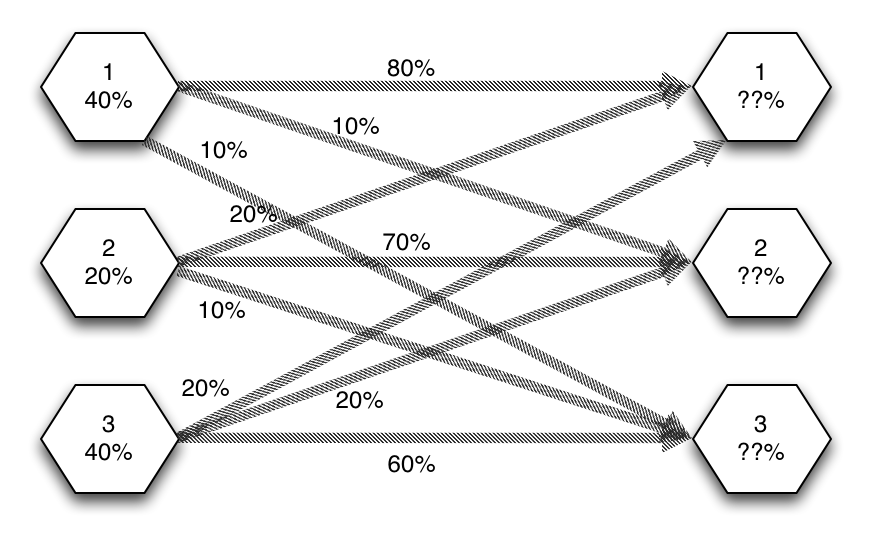
\includegraphics[width=10cm]{marktanteile.png}
\end{frame}

\begin{frame}{Anwendungsbeispiel - Matrizenmultiplikation}
	Darstellung der Marktanteile in den beiden Perioden:
	\[
	\pmb{M^{1}} = \begin{pmatrix}m^{1}_{1}  \\ m^{1}_{2} \\ m ^{1}_{3}\end{pmatrix} = \begin{pmatrix}40 \% \\ 20 \% \\ 40 \%\end{pmatrix} \qquad \pmb{M^{2}} = \begin{pmatrix}m^{2}_{1}  \\ m^{2}_{2} \\ m^{2}_{3}\end{pmatrix}
	\]
	
	Darstellung der Übergänge der Marktanteile durch eine Übergangsmatrix:
	\[
	\pmb{K^{12}} = \begin{pmatrix}
		k^{12}_{11} & k^{12}_{12} & k^{12}_{13} \\
		k^{12}_{21} & k^{12}_{22} & k^{12}_{23} \\
		k^{12}_{31} & k^{12}_{32} & k^{12}_{33} \\
	\end{pmatrix}
	\]
	
	\textbf{$k^{12}_{ij}$ gibt den Anteil des Übergangs von Produzent $j$ auf Produzent $i$ an beim Wechsel von Periode 1 auf Periode 2!}
	
	Die Marktanteile $\pmb{M_{2}}$ in Periode 2 sind dann:
	\[
		\pmb{M^{2}} = \pmb{K^{12}} \pmb{M^{1}}
	\]
\end{frame}

\begin{frame}{Anwendungsbeispiel - Matrizenmultiplikation}
	\[
	\pmb{M^{2}} = \pmb{K^{12}} \pmb{M^{1}} = \begin{pmatrix}
		0,8 & 0,2 & 0,2 \\
		0,1 & 0,7 & 0,2 \\
		0,1 & 0,1 & 0,6
	\end{pmatrix} \begin{pmatrix}
		40\% \\ 20 \% \\ 40 \%
	\end{pmatrix} = \begin{pmatrix}
		44\% \\ 26 \% \\ 30 \%
	\end{pmatrix}
	\]
	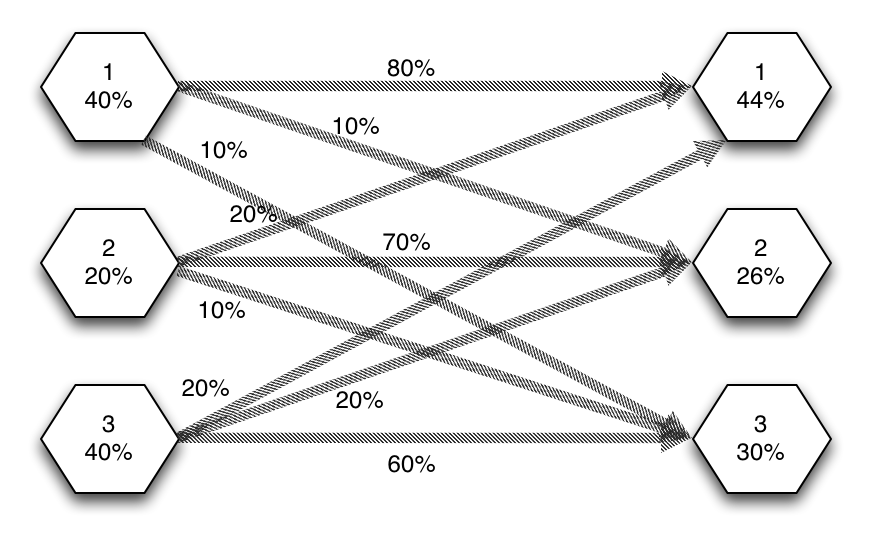
\includegraphics[width=10cm]{marktanteile_ergebnis.png}
\end{frame}

\begin{frame}{Anwendungsbeispiel - Matrizenmultiplikation}
	Bezeichnet $\pmb{K^{23}}$ die entsprechende Übergangsmatrix von Periode 2 auf Periode 3, so kann man die Übergangsmatrix von Periode 1 auf Periode 3 wie folgt berechnen:
	\[
		\pmb{K^{13}} = \pmb{K^{23}} \pmb{K^{12}}
	\]
	denn für die Marktanteile in Periode 3 gilt:
	\[
	\pmb{M^{3}}  = \pmb{K^{13}} \pmb{M^{1}} = \pmb{K^{23}} \pmb{M^{2}} = \pmb{K^{23}} \pmb{K^{12}} \pmb{M^{1}}
	\]
		Mit den Übergangsmatrizen
		\[
		\pmb{K^{12}} = \begin{pmatrix}
		0,8 & 0,2 & 0,2 \\
		0,1 & 0,7 & 0,2 \\
		0,1 & 0,1 & 0,6
		\end{pmatrix} \qquad \mbox{und} \qquad 	\pmb{K^{23}} = \begin{pmatrix}
		0,7 & 0,1 & 0,2 \\
		0,2 & 0,8 & 0,1 \\
		0,1 & 0,1 & 0,7
		\end{pmatrix}
		\]
		
\end{frame}

\begin{frame}{Anwendungsbeispiel - Matrizenmultiplikation}
		\begin{equation*}
		\begin{array}{@{}rl}
		\pmb{K^{12}} \ = \
		\left(
		\begin{array}{c} 0,8 \\ 0,1 \\ 0,1
		\end{array}
		\fbox{$\begin{array}{c} 0,2 \\  0,7 \\ 0,1 \end{array}$}
		\begin{array}{c} 0,2 \\ 0,2 \\ 0,6
		\end{array}
		\right) \, &
		\\
		\pmb{K^{23}} \ = \
		\left(
		\begin{array}{c}
		0,7 \quad 0,1 \quad 0,2 \\
		\fbox{$0,2 \quad 0,8 \quad 0,1$} \\
		0,1 \quad 0,1 \quad 0,7
		\end{array} \right) \
		\left(
		\begin{array}{c} 0,59 \\ 0,25 \\ 0,16 \end{array}
	\begin{array}{c} 0,23 \\ \fbox{0,61} \\ 0,16
		\end{array}
	\begin{array}{c} 0,28 \\ 0,26 \\ 0,46 \end{array}
		\right) &  = \ \pmb{C}
		\end{array}
		\end{equation*}
		
		Damit sind die Marktanteile im dritten Jahr:
		\[
			\pmb{M^{3}} = \pmb{K^{13}} \pmb{M^{1}} = \begin{pmatrix}
				0,59 & 0,23 & 0,28 \\
				0,25 & 0,61 & 0,26 \\
				0,16 & 0,16 & 0,46
			\end{pmatrix} \begin{pmatrix}
				40 \% \\ 20 \% \\ 40 \%
			\end{pmatrix} = \begin{pmatrix}
				39,4 \% \\ 32,6 \% \\ 28 \%
			\end{pmatrix}
		\]
		
\end{frame}

\subsubsection{Determinanten}

\begin{frame}{Determinanten - Motivation}
	Für das $2\times 2$-Gleichungssystem
	\begin{align*}
		a_{11} x_{1} + a_{12} x_{2} = b_{1} \\
		a_{21} x_{2} + a_{22} x_{2} = b_{2}
	\end{align*}
	kann man auch schreiben
	\[
	\pmb{A} \vv{x} =
	\begin{pmatrix}
		a_{11} & a_{12} \\
		a_{21} & a_{22}
	\end{pmatrix} \begin{pmatrix}
	x_{1} \\ x_{2}
	\end{pmatrix} = \begin{pmatrix}
		b_{1} \\ b_{2}
	\end{pmatrix} = \vv{b}
	\]
	oder für das Gauß-Jordan-Verfahren:
	\[
		\left(\begin{array}{cc|c}
			a_{11} & a_{21} & b_{1} \\
			a_{12} & a_{22} & b_{2}
		\end{array}\right)
	\]
\end{frame}

\begin{frame}{Determinanten - Motivation}
	Multipliziert man für das Gauß-Jordan-Verfahren
	\[
	\left(\begin{array}{cc|c}
	a_{11} & a_{21} & b_{1} \\
	a_{12} & a_{22} & b_{2}
	\end{array}\right)
	\]
	\begin{itemize}
	\item die erste Zeile mit $a_{22}$ und die zweite Zeile mit $a_{12}$ und subtrahiert die beiden Ergebnisse für die erste Zeile
	\item die zweite Zeile mit $a_{11}$ und die erste Zeile mit $a_{21}$ und subtrahiert die beiden Ergebnisse für die zweite Zeile,
	\end{itemize}
	so erhält man:
	\[
	\left(\begin{array}{cc|c}
	a_{11}a_{22} - a_{12}a_{12} & 0  & a_{22}b_{1} - a_{12}b_{2} \\
	0 & a_{11}a_{22} - a_{12}a_{12} & a_{11}b_{2} - a_{21}b_{1}
	\end{array}\right)
	\]
	Das hat schon Diagonalform und die Faktoren vor $x_{1}$ und $x_{2}$ sind gleich, nämlich die \textbf{Determinante von $\pmb{A}$}
	
	\fbox{$ \det \pmb{A} := a_{11} a_{22} - a_{12} a_{21}$}
\end{frame}

\begin{frame}{Determinante - Definition $2 \times 2$}
	\begin{definition}
		Die \textbf{Determinante} ist eine reelle Zahl, die aus den Elementen einer \emph{quadratischen Matrix} nach bestimmten Vorschriften berechnet wird.
		
		Diese Zahl ist nützlich u.a. für die Entscheidung über die Lösbarkeit von linearen Gleichungssystemen.
	\end{definition}
	\begin{definition}
		Für eine quadratische $2 \times 2$-Matrix
		\[
			\pmb{A} = 	\begin{pmatrix}
			a_{11} & a_{12} \\
			a_{21} & a_{22}
			\end{pmatrix}
		\]
		ist die Determinante
		\[
		\det \pmb{A} := \det \begin{vmatrix}
		a_{11} & a_{12} \\
		a_{21} & a_{22}
		\end{vmatrix} := a_{11} a_{22} - a_{21} a_{12}
		\]
	\end{definition}
\end{frame}

\begin{frame}{Determinante - Definition $3 \times 3$}
	\begin{definition}
		Für eine $3 \times 3$-Matrix \[
		\pmb{A} = \begin{pmatrix}
		a_{11} & a_{12} & a_{13} \\
		a_{21} & a_{22} & a_{23} \\
		a_{31} & a_{32} & a_{33}
		\end{pmatrix}
		\]
		lautet die Determinante $\det A$
		\fbox{
		{\scriptsize
		$a_{11} a_{22} a_{33} + a_{12} a_{23} a_{31} + a_{13} a_{21} a_{32} - a_{31} a_{22} a_{13} - a_{32} a_{23} a_{11} - a_{33} a_{21} a_{12} $ } }
	\end{definition}
\end{frame}

\begin{frame}{Determinanten - Regel von Sarrus für $3 \times 3$-Determinanten}
	\begin{bemerkung}
	Für $3 \times 3$-Matrizen läßt sich die Formel für die Determinante mit der Regel von Sarrus herleiten:
\begin{center}
\begin{tikzpicture}
\matrix [%
matrix of math nodes,column sep=1em,row sep=1em,ampersand replacement=\& ] (sarrus) {%
	a_{11} \& a_{12} \& a_{13} \& a_{11} \& a_{12} \\
	a_{21} \& a_{22} \& a_{23} \& a_{21} \& a_{22} \\
	a_{31} \& a_{32} \& a_{33} \& a_{31} \& a_{32} \\
};

\path ($(sarrus-1-3.north east)+(0.5em,0)$) edge[dotted] ($(sarrus-3-3.south east)+(0.5em,0)$)
(sarrus-1-1)                          edge         (sarrus-2-2)
(sarrus-2-2)                          edge         (sarrus-3-3)
(sarrus-1-2)                          edge         (sarrus-2-3)
(sarrus-2-3)                          edge         (sarrus-3-4)
(sarrus-1-3)                          edge         (sarrus-2-4)
(sarrus-2-4)                          edge         (sarrus-3-5)
(sarrus-3-1)                          edge[dashed] (sarrus-2-2)
(sarrus-2-2)                          edge[dashed] (sarrus-1-3)
(sarrus-3-2)                          edge[dashed] (sarrus-2-3)
(sarrus-2-3)                          edge[dashed] (sarrus-1-4)
(sarrus-3-3)                          edge[dashed] (sarrus-2-4)
(sarrus-2-4)                          edge[dashed] (sarrus-1-5);

\foreach \c in {1,2,3} {\node[anchor=south] at (sarrus-1-\c.north) {$+$};};
\foreach \c in {1,2,3} {\node[anchor=north] at (sarrus-3-\c.south) {$-$};};
\end{tikzpicture}
\end{center}
\end{bemerkung}
\end{frame}

\begin{frame}{Determinantenentwicklungssatz von Laplace}
	Für die Berechnung von Determinanten von Matrizen mit mehr Spalten (bzw. Zeilen) braucht man den \textbf{Entwicklungssatz von Laplace}:
	\begin{theorem}
		Die Determinante einer $(n \times n)$-Matrix $\pmb{A}$ kann mit dem Entwicklungß atz von Laplace berechnet werden:
		\[
		\det \pmb{A} = \sum\limits_{k=1}^{n} (-1)^{i+k} a_{ik} \det A_{ik} = \sum\limits_{i=1}^{n} (-1)^{i+k} a_{ik} \det A_{ik}
		\]
		wobei
		\begin{itemize}
		\item $i$ für eine beliebige Zeile bzw. $k$ für eine beliebige Spalte steht und
		\item $A_{ik}$ die Matrix bezeichnet, die entsteht, wenn man in der Matrix $\pmb{A}$ die $i$-te Zeile und die $k$-te Spalte streicht, und deren Determinante man \textbf{Unterdeterminanten} oder (zusammen mit dem Vorfaktor $(-1)^{i+k}$) \textbf{Adjunkte} nennt.
		\end{itemize}
	\end{theorem}
\end{frame}

\begin{frame}{Determinantenentwicklungssatz von Laplace}
	\begin{bemerkung}
		\begin{itemize}
			\item Für die Vorfaktoren $(-1)^{i+k}$ kann man sich am besten die Matrix wie folgt in Schachbrettform vorstellen:
			\[
				\begin{vmatrix}
				+ & - & + & - & + & \cdots \\
			    - & + & - & + & - & \cdots \\
				+ & - & + & - & + & \cdots \\
				- & + & - & + & - & \cdots \\
				\vdots & \vdots & \vdots & \vdots & \vdots & \ddots
				\end{vmatrix}
			\]
			\item Die im Entwicklungssatz vorkommenden Determinanten der Matrizen $A_{ik}$ sind Determinanten von kleineren $(n-1) \times (n-1)$-Matrizen, die man entweder wieder mit dem Entwicklungssatz, der Regel von Sarrus oder einfacher berechnen kann.
			\item Man entwickelt also entweder nach einer Zeile ($i$ bleibt, einmal gewählt, fest) oder nach einer Spalte ($k$ bleibt fest).
		\end{itemize}
	\end{bemerkung}
\end{frame}

\begin{frame}{Determinantenentwicklungssatz von Laplace}
	\begin{bemerkung}
	\begin{itemize}
		\item Idealerweise entwickelt man nach der Zeile oder Spalte, in der möglichst viele 0 vorkommen, weil so die entsprechenden Summenterme wegfallen und damit die Berechnung der entsprechenden Unterdeterminanten.
		\item Man kann vor der Berechnung die Matrix mit den Umformungen aus dem Gauß-Verfahren so verändern, dass in einer Zeile oder Spalte alle Elemente bis auf eines 0 sind bzw. möglichst viele 0 entstehen.
		\item Für eine Dreiecksmatrix (sie muss nicht diagonal sein), die also alle Einträge unterhalb oder oberhalb der Diagonalen 0 hat, muss  man nur die Einträge in der Diagonalen multiplizieren. Das gilt dann natürlich auch für Diagonalmatrizen.
		\item Wenn eine Zeile oder eine Spalte vollständig aus 0 besteht, ist die Determinanten automatisch auch 0.
	\end{itemize}
	\end{bemerkung}
\end{frame}

\begin{frame}{Determinantenentwicklungssatz - Beispiel}
	Im folgenden Beispiel entwickelt man am besten nach der dritten Zeile:
	\[
	\begin{vmatrix}
	1 & 2 & 5 & 3 \\
	2 & -1 & 6 & 7 \\
	1 & 0 & 0 & 2 \\
	-2 & -3 & 1 & 2
	\end{vmatrix} = 1 \cdot \begin{vmatrix}
	2 & 5 & 3 \\
	-1 & 6 & 7 \\
	-3 & 1 & 2
	\end{vmatrix} - 2 \cdot \begin{vmatrix}
	1 & 2 & 5 \\
	2 & -1 & 6 \\
	-2 & -3 & 1
	\end{vmatrix}
	\]
	\[
	 = 1\cdot(-34) -2\cdot(-51) = 102 - 34 = 68 \]
\end{frame}

\begin{frame}{Rechenregeln für Determinanten}
	Für Determinanten gelten einige Rechenregeln:
	\begin{itemize}
		\item Vertauscht man zwei Zeilen oder zwei Spalten einer Determinante, so ändert die Determinante ihr Vorzeichen.
		\item Multipliziert man eine $n \times n$-Matrix mit einer Zahl $\lambda$, so ist die Determinante mit der $n$-fachen Potenz von $\lambda$ zu multiplizieren:
		\[
		\det \left( \lambda \pmb{A} \right) = \lambda^{n} \det \pmb{A}
		\]
		\item Die Addition oder Subtraktion des Vielfachen einer Zeile oder Spalte zu einer anderen Zeile oder Spalte ändert den Wert der Determinanten nicht.
		\item Das Transponieren einer Matrix ändert die Determinante nicht, d.h.
		\[
		\det \pmb{A} = \det \pmb{A^{T}}
		\]
		\item Die Determinate eines Matrizenproduktes ist der Produkt der Determinante der Multiplikatoren:
		\[
		\det \left(\pmb{A} \pmb{B}\right) = \det \pmb{A} \det \pmb{B}
		\]
	\end{itemize}
\end{frame}

\begin{frame}{Determinanten und Lösbarkeit von LGS}
	\begin{definition}
		Eine $n \times n$-Matrix $\pmb{A}$ heißt \textbf{regulär} oder \textbf{invertierbar}, wenn für ihre Determinante
		\[
		\det \pmb{A} \neq 0
		\]
		gilt.
		Eine Matrix $\pmb{A}$, deren Determinante $\det \pmb{A} = 0$ ist, heißt \textbf{singulär}.
	\end{definition}
	Für die Lösbarkeit eines linearen Gleichungssystems $\pmb{A}\vv{x} = \vv{b}$ gibt es vier mögliche Fälle:
	\small{
	\begin{tabular}{|c|c|c|}
		\hline
		& homogen $\vv{b}=0$ & inhomogen $\vv{b} \neq 0$ \\
		\hline
		$\det \pmb{A} = 0$ & unendlich viele Lösungen & unendlich viele oder keine Lösung \\
		\hline
		$\det \pmb{A} \neq 0$ & genau eine Lösung $\vv{x}=0$ & genau eine Lösung $\vv{x} \neq 0$\\
		\hline
	\end{tabular}}
\end{frame}

\begin{frame}{Lösung linearer Gleichungssysteme - Cramersche Regel}
	\begin{theorem}
	Für die Lösung $\vv{x}$ eines (quadratischen) linearen Gleichungssystems $\pmb{A} \vv{x} = \vv{b}$ mit regulärer Koeffizientenmatrix $\pmb{A}$ gilt:
	\[
	x_{i} = \frac{\det \pmb{A_{i}}}{\det \pmb{A}}
	\]
	wobei die Matrizen $\pmb{A_{i}}$ aus $\pmb{A}$ hervorgehen, indem man die $i$-te Spalte der Matrix $\pmb{A}$ durch den Vektor $\vv{b}$ ersetzt.
 	\end{theorem}
\end{frame}

\begin{frame}{Cramersche Regel - Beispiel}
	Für das lineare Gleichungssystem
	
		\begin{align*}
		- x_{1}  + x_{2}  + x_{3} & =  0 \\
		x_{1}  -3 x_{2}  -2 x_{3} & =  5 \\
		5 x_{1}  +x_{2}  +4 x_{3} & =  3
		\end{align*}

	oder in Matrixschreibweise
	\[
	\begin{pmatrix}
	-1 & 1 & 1 \\
	1 & -3 & -2 \\
	5 & 1 & 4
	\end{pmatrix} \cdot \begin{pmatrix}x_{1} \\ x_{2} \\ x_{3} \end{pmatrix} = \begin{pmatrix}
	0 \\ 5 \\ 3
	\end{pmatrix}
	\]
	ist
	\[
	\pmb{A}= \begin{pmatrix}
	-1 & 1 & 1 \\
	1 & -3 & -2 \\
	5 & 1 & 4
	\end{pmatrix}
	\qquad
	\vv{b} = \begin{pmatrix}
	0 \\ 5 \\ 3
	\end{pmatrix}
	\]
\end{frame}

\begin{frame}{Cramersche Regel - Beispiel}
		\[
		\pmb{A}= \begin{pmatrix}
		-1 & 1 & 1 \\
		1 & -3 & -2 \\
		5 & 1 & 4
		\end{pmatrix}
		\qquad
		\vv{b} = \begin{pmatrix}
		0 \\ 5 \\ 3
		\end{pmatrix}
		\]
		und daher \footnotesize{
		\[
		\pmb{A_1}= \begin{pmatrix}
		0 & 1 & 1 \\
		5 & -3 & -2 \\
		3 & 1 & 4
		\end{pmatrix}
		\qquad
		\pmb{A_2}= \begin{pmatrix}
		-1 & 0 & 1 \\
		1 & 5 & -2 \\
		5 & 3 & 4
		\end{pmatrix}
		\qquad
		\pmb{A_3}= \begin{pmatrix}
		-1 & 1 & 0 \\
		1 & -3 & 5 \\
		5 & 1 & 3
		\end{pmatrix}
		\]
		}
		und mit der Regel von Sarrus
		\[
		\det \pmb{A_1} = -12 \qquad \det \pmb{A_2} = -48
 \qquad \det \pmb{A_3} = 36 \qquad \det \pmb{A} = 12		
 \]
	und daher
	\[
	x_{1} = \frac{-12}{12} = -1 \qquad x_{2} = \frac{-48}{12} = -4 \qquad x_{3} = \frac{36}{12} = 3
	\]	
\end{frame}

%\section{Analysis - Folgen und Reihen}
\subsection{Folgen}
\subsubsection{Folgen und Grenzwerte}
\begin{frame}{Folgen}
	\begin{definition}
		Eine \textbf{reellwertige Folge} $(a_{n})_{n \in \mathbb{N}}$ ist eine Abbildung von $\mathbb{N}$ in $\mathbb{R}$, d. h. jedem $n \in \mathbb{N}$ wird eine reelle Zahl $a_{n} \in \mathbb{R}$ zugeordnet.
		
		Falls $a_{n} = c$ für alle $n \in \mathbb{N}$ und eine feste Zahl $c$, so heißt die Folge $(a_{n})_{n \in \mathbb{N}}$ \textbf{konstante Folge}.
		
		Eine Folge, für die $a_{n+1} = q \cdot a_{n}$ erfüllt ist für alle $n \in \mathbb{N}$, heißt \textbf{geometrische Folge}.
	\end{definition}
	\begin{example}
		Beispiele für Folgen sind:
		\begin{align*}
			(a_{n})_{n \in \mathbb{N}} = (n)_{n \in \mathbb{N}} & \mbox{ also } (1, 2, 3, 4, 5, 6, \ldots) \\
			(a_{n})_{n \in \mathbb{N}} = \left(\frac{1}{n}\right)_{n \in \mathbb{N}} & \mbox{ also } (1, \frac{1}{2}, \frac{1}{3}, \frac{1}{4}, \frac{1}{5}, \frac{1}{6}, \ldots) \\
			(a_{n})_{n \in \mathbb{N}} = \left((-1)^{n}\frac{1}{n}\right)_{n \in \mathbb{N}} & \mbox{ also } (-1, \frac{1}{2}, -\frac{1}{3}, \frac{1}{4}, -\frac{1}{5}, \frac{1}{6}, \ldots)	
		\end{align*}
	\end{example}
\end{frame}

\begin{frame}{Beispiele für Folgen}
	\begin{definition}
		Die Folge
		\[
		a_{n} := \frac{1}{n} \mbox{ mit } \left(a_{n}\right) = \left(\frac{1}{1}, \frac{1}{2}, \frac{1}{3}, \frac{1}{4}, \ldots \right)
		\] heißt \textbf{harmonische Folge}.
	\end{definition}
	
\end{frame}

\begin{frame}{Beispiele rekursiv definierter Folgen}
		Man kann folgen auch \textbf{rekursiv} definieren. 
	\begin{example}
		Die \textbf{Fibonacci-Folge} wird definiert als:
		\[
			a_{1} := 1 \qquad a_{2} := 1 \qquad a_{n} := a_{n-1} + a_{n-2} \mbox{ für } n \geq 3
		\]
		also 
		\[
			 \left( a_{n} \right) = \left( 1, 1, 2, 3, 5, 8, 13, 21, \ldots \right) 
		\]
	\end{example}
	\begin{example}
		Für die Folge
		\[
		a_{1} := 1 \qquad a_{n} := n \cdot a_{n-1} \mbox{ für } n \geq 2
		\]
		ist die Folge der Fakultäten:
		\[
			a_{n} = n!
		\]
	\end{example}
\end{frame}

\begin{frame}{Numerische Berechnung von Wurzeln}
	\begin{example}
		Für eine Zahl $x > 0$ sei $a_{1} := 1$ und
		\[
			a_{n+1} := \frac{1}{2} \left( a_{n} + \frac{x}{a_{n}} \right) \mbox{ für alle } n \geq 1 
		\]
		Diese Folge nennen wir hier \textbf{Heron-Folge zur Zahl $x$}.
	\end{example} 
\end{frame}

\begin{frame}{Folgen}
	\begin{bemerkung}
		Es gibt auch allgemeinere Folgen, die jedem $n \in \mathbb{N}$ ein Element einer beliebigen Menge $M$ zuordnet.
		
		Die Zahlen bzw. Elemente $a_{n}$ heißen \textbf{Glieder der Folge}.
		
		Folgen können beliebige Abfolgen von Elementen der Bildmenge $M$ (hier immer $\mathbb{R}$) sein. Falls es aber eine Regel gibt, nach der die Folgenglieder berechnet werden, nennt man diese Regel das \textbf{Bildungsgesetz der Folge}.
	\end{bemerkung}
\end{frame}

\begin{frame}{Eigenschaften von Zahlenfolgen}
	\begin{definition}
		Eine Folge $(a_{n})_{n \in \mathbb{N}}$ heißt
		\begin{itemize}
			\item \textbf{nach oben beschränkt}, wenn es eine Zahl $M$ gibt, sodass $a_{n} < M$ für alle $n \in \mathbb{N}$.
			\item \textbf{nach unten beschränkt}, wenn es eine Zahl $m$ gibt, sodass $m < a_{n}$ für alle $n \in \mathbb{N}$.
			\item \textbf{beschränkt}, wenn sie nach oben und nach unten beschränkt ist.
			\item \textbf{unbeschränkt}, wenn sie nicht beschränkt ist.
			\item \textbf{streng monoton steigend}, wenn $a_{n+1}>a_{n}$ für alle $n \in \mathbb{N}$.
			\item \textbf{monoton steigend}, wenn $a_{n+1}\geq a_{n}$ für alle $n \in \mathbb{N}$.
			\item \textbf{streng monoton fallend}, wenn $a_{n+1}<a_{n}$ für alle $n \in \mathbb{N}$.
			\item \textbf{monoton fallend}, wenn $a_{n+1}\leq a_{n}$ für alle $n \in \mathbb{N}$.
			\item \textbf{alternierend}, wenn $a_{n} \cdot a_{n+1} < 0$ für alle $n \in \mathbb{N}$, d. h. die Vorzeichen benachbarter Folgenglieder wechseln.
		\end{itemize}
	\end{definition}
\end{frame}

\begin{frame}{Eigenschaften von Zahlenfolgen}
	\begin{definition}
		Eine Zahl $h$ heißt \textbf{Häufungspunkt der Folge} $(a_{n})_{n \in \mathbb{N}}$, wenn für jedes $\varepsilon>0$ 
		\[
			\left| a_{n} - h \right| < \varepsilon
		\]
		für \textbf{unendlich} viele Folgenglieder gilt.
		
		Das heißt anschaulich: Egal wie nah man $h$ kommt, es gibt immer noch unendlich viele Folgenglieder, die noch näher an $h$ liegen.
		
		Hat eine Folge \textbf{genau einen} Häufungspunkt $h$, so nennt man die Folge \textbf{konvergent} und $h$ den \textbf{Grenzwert} der Folge und man schreibt:
		\[
			\lim_{n \to \infty} a_{n} = h
		\]
		
		Eine \textbf{nicht konvergente} Folge heißt \textbf{divergent}.
	\end{definition}
\end{frame}

\begin{frame}{Konvergenz von Folgen}
	\begin{theorem}
		Eine Folge ist genau dann kovergent gegen $h \in \mathbb{R}$, wenn es zu jedem $\varepsilon > 0$ eine Zahl $N(\varepsilon) \in \mathbb{N}$ gibt, sodass
		\[
			\left| a_{n} - h \right| < \varepsilon \qquad \forall n > N(\varepsilon)
		\]  
	\end{theorem}
	\begin{bemerkung}
		Eine konvergente Folge, deren Grenzwert $h = 0$ ist, heißt \textbf{Nullfolge}.
		
		Wächst eine Zahlenfolge über alle Grenzen, so schreibt man:
		\[
		\lim_{n \to \infty} a_{n} = \infty
		\]
	\end{bemerkung}
\end{frame}

\begin{frame}{Konvergenz und Monotonie}
	\begin{theorem}
		Jede \textbf{beschränkte und monotone} Zahlenfolge ist \textbf{konvergent}.
	\end{theorem}
	\begin{bemerkung}
		Beide Bedingungen (Beschränktheit und Monotonie) sind wichtig, eine allein reicht (noch) nicht aus für die Konvergenz einer Folge.
	\end{bemerkung}
\end{frame}

\begin{frame}{Rechenregeln für Grenzwerte}
	\begin{theorem}
		Es gilt für zwei \textbf{konvergente} Folgen $(a_{n})_{n \in \mathbb{N}}$ und $(b_{n})_{n \in \mathbb{N}}$ mit 
		\[
		\lim_{n \to \infty} a_{n} = a \mbox{  und  } \lim_{n \to \infty} b_{n} = b
		\] 
		\begin{itemize}
			\item Die \textbf{Summenfolge} $(c_{n})_{n \in \mathbb{N}}$ mit $c_{n} := a_{n} + b_{n}$ konvergiert und:
			\[
			\lim_{n \to \infty} c_{n} = \lim_{n \to \infty} a_{n} + b_{n} = \lim_{n \to \infty} a_{n} + \lim_{n \to \infty} b_{n} = a + b
			\]
			\item Die Folge $d_{n} := c \cdot a_{n}$ mit einer Konstanten $c \in \mathbb{R}$  konvergiert:
			\[
			\lim_{n \to \infty} d_{n} = \lim_{n \to \infty} c \cdot a_{n} = c \cdot a
			\]
			\item Die \textbf{Produktfolge} $(p_{n})_{n \in \mathbb{N}}$ mit $p_{n} := a_{n} \cdot b_{n}$ konvergiert mit:
			\[
			\lim_{n \to \infty} p_{n} = \lim_{n \to \infty} a_{n} \cdot b_{n} = \lim_{n \to \infty} a_{n} \cdot \lim_{n \to \infty} b_{n} = a \cdot b
			\]
		\end{itemize}
	\end{theorem}
\end{frame}

\begin{frame}{Rechenregeln für Grenzwerte}
	\begin{bemerkung}
		Aus dem vorherigen Satz folgt für zwei \textbf{konvergente} Folgen $(a_{n})_{n \in \mathbb{N}}$ und $(b_{n})_{n \in \mathbb{N}}$ auch:
		\begin{itemize}
			\item Die Differenzfolge konvergiert:
			\[
			\lim_{n \to \infty} (a_{n} - b_{n}) = \lim_{n \to \infty} a_{n} - \lim_{n \to \infty} b_{n} = a - b
			\]
			\item Sind alle $b_{n} \neq 0$ und $b \neq 0$, so konvergiert auch die \textbf{Quotientenfolge}:
			\[
			\lim_{n \to \infty} \frac{a_{n}}{b_{n}} = \frac{\lim_{n \to \infty} a_{n}}{\lim_{n \to \infty} b_{n}} = \frac{a}{b}
			\]
%						
		\end{itemize}
	\end{bemerkung}
\end{frame}

\begin{frame}{Beispiele für die Berechnung von Grenzwerten}
	\begin{example}
	\begin{align*}
		& \lim_{n \to \infty} \frac{2n}{n+1} = \lim_{n \to \infty} \frac{2n+2 - 2}{n+1}  = \lim_{n \to \infty} \frac{2(n+1) - 2}{n+1} \\ & = \lim_{n \to \infty} \left( 2 - \frac{2}{n+1} \right) = \lim_{n \to \infty} 2 - \lim_{n \to \infty} \frac{2}{n+1}  = 2 - 0   = 2 \\
		& \lim_{n \to \infty} \cos \left( 2- \frac{1}{n} \right)  = \cos 2 \\
		& \lim_{n \to \infty} (-1)^{n} \left( 1 + \frac{1}{n}  \right) \mbox{ existiert nicht! Warum?}
	\end{align*}
	\end{example}
\end{frame}

\begin{frame}{Numerische Berechnung von Wurzeln}
	\begin{theorem}
		Die \textbf{Heron-Folge zur Zahl $x>0$} mit $a_{1} = 1$ und
		\[
		a_{n+1} := \frac{1}{2} \left( a_{n} + \frac{x}{a_{n}} \right) \mbox{ für alle } n \geq 1 		
		\]
		konvergiert und für den Grenzwert gilt:
		\[
			a := \lim_{n \to \infty} a_{n+1} = \lim_{n \to \infty} \frac{1}{2} \left( a_{n} + \frac{x}{a_{n}} \right)
		\]
		und daher für $a$ 
		\[
			a = \frac{1}{2} \left( a + \frac{x}{a} \right)
		\]
		Diese Gleichung hat nur die positive Lösung $a=\sqrt{x}$ und daher:
		\[
			\lim_{n \to \infty} a_{n} = \sqrt{x}
		\]
	\end{theorem}
\end{frame}

\subsubsection{Spezielle Folgen}

\begin{frame}{Arithmetische Folgen}
	\begin{definition}
		Gilt für eine Folge $\left(a_{n}\right)_{n \in \mathbb{N}}$ für alle $n \in \mathbb{N}$:
		\[
		d := a_{n+1} - a_{n} = \mbox{konstant,}
		\]
		so heißt sie \textbf{arithmetische Folge}.
	\end{definition}
\end{frame}	
\begin{frame}{Eigenschaften arithmetischer Folgen}
	\begin{bemerkung}
		\begin{itemize}
		\item Eine arithmetische Folge ist \textbf{eindeutig} durch das Anfangsglied $a_{1}$ und die konstante Differenz $d$ bestimmt und es gilt:
		\[
			a_{n} = a_{1} + d \cdot (n - 1)
		\]
		\item Da für eine arithmetische Folge sowohl
		\[
			d = a_{n+1} - a_{n} \mbox{ als auch } d = a_{n} - a_{n-1}
		\] 
		gilt, ist (durch Gleichsetzen der beiden Gleichungen)
		\[
			a_{n} = \frac{1}{2} \left( a_{n+1} + a_{n-1}\right)
		\]
		also jedes Folgenglied das \textbf{arithemtische Mittel} seiner benachbarten Folgenglieder.
		\end{itemize}	
	\end{bemerkung}
\end{frame}

\begin{frame}{Divergenz/Konvergenz arithmetischer Folgen}
	\begin{theorem}
		Eine \textbf{arithmetische Folge} konvergiert dann und nur dann, wenn $d = a_{n} - a_{n-1} = 0$ ist. In diesem Fall ist die Folge sogar konstant und es gilt:
		\[
		\lim_{n \to \infty} a_{n} = a_{1} = a_{2} = \cdots
		\] 
		
		Gilt für eine arithmetische Folge also $d \neq 0$, dann divergiert die Folge:
		\begin{align*}
			\lim_{n \to \infty} a_{n} & = \infty & \mbox{ falls d > 0} \\
			\lim_{n \to \infty} a_{n} & = - \infty & \mbox{ falls d < 0}
		\end{align*}
	\end{theorem}
\end{frame}

\begin{frame}{Geometrische Folgen}
	\begin{definition}
		Eine Folge $(a_{n})_{n \in \mathbb{N}}$ heißt \textbf{geometrische Folge}, wenn 
		\[
		\frac{a_{n+1}}{a_{n}} = q = \mbox{const. für alle } n \in \mathbb{N}   
		\]
		ist.
	\end{definition}
\end{frame}	
\begin{frame}{Eigenschaften geometrischer Folgen}
	\begin{bemerkung}
		\begin{itemize}
		\item Eine geometrische Folge ist eindeutig durch ihr Anfangsglied $a_{1}$ und den konstanten Quotienten $q$ bestimmt und es gilt:
		\[
			a_{n} = a_{1} \cdot q^{n-1}
		\]
		\item Da für eine geometrische Folge sowohl
		\[
		q = \frac{a_{n+1}}{a_{n}} \mbox{ als auch } q = \frac{a_{n}}{a_{n-1}}
		\]
		gilt, ist  (durch Gleichsetzen der beiden Gleichungen)
		\[
			a_{n} = \sqrt{a_{n-1} \cdot a_{n+1}}
		\]
		also jedes Folgenglied das \textbf{geometrische Mittel} seiner benachbarten Folgenglieder.
		\end{itemize} 
	\end{bemerkung}
\end{frame}

\begin{frame}{Konvergenz/Divergenz geometrischer Folgen}
	\begin{bemerkung}
	Bezüglich der Konvergenz bzw. Divergenz einer geometrischen Folge $a_{n} = a_{1} q^{n-1}$ gilt folgende Fallunterscheidung:
	\begin{itemize}
		\item Falls $|q| < 1$ ist, so konvergiert die Folge gegen 0. 
		\[
		\lim_{n \to \infty} a_{n} = \lim_{n \to \infty} a_{1} q^{n-1} = 0
		\]
		\item Falls $q\leq-1$ ist, so ist die Folge alternierend und divergent.
		\item Falls $q>1$ ist, so ist die Folge divergent.
		\item Falls $q=1$ ist, so konvergiert die Folge, weil sie konstant ist: $\lim_{n \to \infty} a_{n} = \lim_{n \to \infty} a_{1} \cdot 1^{n-1} = a_{1}$.
	\end{itemize}
	\end{bemerkung}	
\end{frame}

\begin{frame}{Techniken zum Nachweis von Beschränktheit und Monotonie}
	\begin{itemize}
		\item Sind alle Folgenglieder positiv bzw. negativ? Falls ja: Die Folge ist durch 0 nach oben bzw. nach unten beschränkt.
		\item Gilt $a_{n+1} - a_{n} \geq 0$ oder $a_{n+1} - a_{n} > 0$? Falls ja: Die Folge ist monoton wachsend bzw. streng monoton wachsend.
		\item Gilt $a_{n+1} - a_{n} \leq 0$ oder $a_{n+1} - a_{n} < 0$? Falls ja: Die Folge ist monoton fallend bzw. streng monoton fallend.
		\item Gilt $\frac{a_{n+1}}{a_{n}} \geq 1$ oder $\frac{a_{n+1}}{a_{n}} > 1$? Falls ja: Die Folge ist monoton wachsend bzw. streng monoton wachsend.
		\item Gilt $\frac{a_{n+1}}{a_{n}} \leq 1$ oder $\frac{a_{n+1}}{a_{n}} < 1$? Falls ja: Die Folge ist monoton fallend bzw. streng monoton fallend.
	\end{itemize}
\end{frame}

\begin{frame}{Berechnung von Grenzwerten - Beispiele}
	\begin{example}
		\begin{align*}
		\lim_{n \to \infty} \frac{2}{n} + \left(\frac{1}{3}\right)^{n} +7 & = 7 \\
		\lim_{n \to \infty} \frac{3n^{2} +7n + 8}{5n^{2} -8n +1} & = \frac{3}{5} \\
		\lim_{n \to \infty} \frac{a_{r} n^{r} + \ldots + a_{1} n + a_{0}}{b_{s} n^{s} + \ldots + b_{1} n + b_{0}} & = \begin{cases}
		0 & \text{falls } r <s \\
		+\infty & \text{falls } s<r \text{ und } \frac{a_{r}}{b_{s}} > 0 \\
		-\infty & \text{falls } s<r \text{ und } \frac{a_{r}}{b_{s}} < 0 \\
		\frac{a_{r}}{b_{s}} & \text{falls s=r} \\
		\end{cases} \\
		\lim_{n \to \infty} \sqrt{n^{2}+3n+3} -n & = \frac{3}{2} \\
		\lim_{n \to \infty} \frac{n}{2^{n}} = 0
 		\end{align*}
	\end{example}
\end{frame} 

\begin{frame}{Grenzwertbestimmung bei rekursiv definierten Folgen}
	\begin{bemerkung}
	Falls eine Folge $(a_{n})$ rekursiv definiert wird (wie z.B. die Heron-Folge), bestimmt man den Grenzwert in der Regel wie folgt:
	\begin{itemize}
		\item Man zeigt, dass die Folge konvergiert z.B. durch
		\begin{itemize}
			\item $(a_{n})$ ist beschränkt und
			\item $(a_{n})$ ist monoton.
		\end{itemize}
		\item Man ersetzt in der Rekursionsvorschrift alle $a_{n+1}$, $a_{n}$ usw. durch den zu berechnenden Grenzwert $a$ und erhält damit eine sogenannte Fixpunktgleichung für a.
		\item Man löst die Fixpunktgleichung aus dem vorherigen Schritt.
 	\end{itemize}
	\end{bemerkung}
\end{frame}

\begin{frame}{Grenzwertberechnung rekursiv definierter Folgen}
	\footnotesize{
	\begin{example}
		Für die Folge $a_{n}$ mit
		\[
			a_{1} := 0 \qquad a_{n+1} = \sqrt{2 a_{n}}
		\]
		gilt:
		\begin{itemize}
			\item $a_{n}$ konvergiert, weil $a_{n}$ einerseits beschränkt ist, denn $0  \leq a_{1} \leq 2$ und daher für alle $n$
			\[
				0 \leq a_{n+1} = \sqrt{2 a_{n}} = \sqrt{2} \sqrt{a_{n}} \leq \sqrt{2} \sqrt{2} = 2 
			\]
			und andererseits monton wachsend ist:
			\[
				\frac{a_{n+1}}{a_{n}} = \frac{\sqrt{2a_{n}}}{a_{n}} = \sqrt{\frac{2}{a_{n}}} \geq 1
			\]
			\item Die Fixpunktgleichung lautet dann
			\[
				a = \sqrt{2a}
			\] 
			und hat die Lösungen $a=0$ und $a=2$. Da $a_{n}$ monoton wächst und $a_{1} = 1$ ist, muss der Grenzwert $a=2$ sein.
		\end{itemize}
	\end{example}
}
\end{frame}

\subsection{Reihen}

\begin{frame}{Reihen - Definition}
	\begin{definition}
	Für eine beliebige Zahlenfolge $(a_{n})_{n \in \mathbb{N}}$ heißt die Folge der \textbf{Partialsummen} $(s_{n})_{n \in \mathbb{N}}$ mit dem Bildungsgesetz
	\[
		s_{n} := \sum_{i=1}^{n} a_{i}
	\]
	eine \textbf{unendliche Reihe}.
	
	Konvergiert die Folge der Partialsummen $(s_n)$, so heißt die Reihe \textbf{konvergent}. Ansonsten heißt die Reihe \textbf{divergent}.
	
	Konvergiert die Reihe $(s_{n})$, so nennt man ihren Grenzwert 
	\[
		\lim_{n \to \infty} s_{n} = \lim_{n \to \infty} \sum_{i=1}^{n} a_{i} =: \sum_{i=1}^{\infty} a_{i} 
 	\]
 	den \textbf{Wert der Reihe}.
	\end{definition}	
\end{frame}

\begin{frame}{Beispiele für Reihen}
	\begin{example}
		Die \textbf{geometrische Reihe} ist definiert als Folge der Partialsummen der geometrischen Folge 
		\[
			\sum_{i=1}^{n} a_{1} q^{i-1} = a_{1} \sum_{i=1}^{n} q^{i-1} = a_{1} \left( 1 + q + q^{2} + q^{3} + q^{4} + \ldots + q^{n-1}\right)
		\]
	\end{example}
	\begin{example}
		Die Reihe 
		\[
			s_{n}:= \sum_{k=1}^{n} \frac{1}{k(k+1)} = \sum_{k=1}^{n} \left( \frac{1}{k} - \frac{1}{k+1} \right) = 1 - \frac{1}{n+1}
		\] 
		ist offenbar auch explizit als Folge mit $s_{n} = 1-\frac{1}{n+1}$ definiert. An dieser Reihe kann man das wichtige Prinzip \textbf{der Teleskopsummen} erkennen.
	\end{example}
\end{frame}

\begin{frame}{Beispiele für Konvergenz von Reihen}
	\begin{example}
		Die \textbf{harmonische Reihe} divergiert:
		\[
			\sum_{i=1}^{n} \frac{1}{i} = 1 + \frac{1}{2} + \frac{1}{3} + \ldots + \frac{1}{n}
		\] 
		Dagegen konvergiert die \textbf{alternierende harmonische Reihe} 
		\[
			\sum_{i=1}^{n} (-1)^{i+1} \frac{1}{i} = 1 - \frac{1}{2} + \frac{1}{3} - \ldots + (-1)^{n} \frac{1}{n} = \ln 2
		\]
	\end{example}
\end{frame}

\begin{frame}{Konvergenz von Reihen - Notwendige Bedingung}
	\begin{bemerkung}
		\textbf{Notwendig} für die Konvergenz der Reihe $(s_{n})$ ist, dass die Folge der Summanden $(a_{n})$ eine \textbf{Nullfolge} ist, also 
		\[
			\lim_{n \to \infty} s_{n} = \lim_{n \to \infty} \sum_{i=1}^{n} a_{i} \mbox{ konvergiert} \qquad \Rightarrow \lim_{n \to \infty} a_{n} = 0 
		\]
		Diese Bedingung ist aber \textbf{nicht hinreichend}, denn die harmonische Folge 
		\[
			a_{n} = \frac{1}{n} 
		\]
		konvergiert zwar gegen 0, aber die Reihe
		\[
			\sum_{i=1}^{n} a_{i} = \sum_{i=1}^{n} \frac{1}{i} \mbox{ divergiert.}
		\]
	\end{bemerkung}
\end{frame}

\begin{frame}{Arithmetische  Reihe}
	\begin{definition}
		Die Folge der Partialsummen/Teilsummen einer arithmetischen Folge $a_{n} = a_{1} + d (n-1)$, also
		\[
			s_{n} = \sum_{i=1}^{n} a_{i} = \sum_{i=1}^{n} a_{1} + d (i-1)
		\]
		heißt \textbf{arithmetische Reihe} und hat die Summenformel
		\[
			s_{n} = \frac{n}{2}	\left( a_{1} + a_{n} \right) = \frac{n}{2} \left( 2 a_{1} + d (n-1)  \right)
		\]
	\end{definition}
	\begin{bemerkung}
		Die Summenformel hat Carl Friedrich Gauß angeblich als 10-jähriger Schüler gefunden, als er zur Strafe die Zahlen von 1 bis 100 addieren sollte, was eine arithmetische Folge von Zahlen mit $a_{1}=1$ und $d=1$ ist.
	\end{bemerkung}
\end{frame}

\begin{frame}{Arithmetische  Reihe - Gauß}
	\begin{example}
		Die Summenformel hat Gauß so hergeleitet:
		\begin{align*}	
			s_{n} & = a_1  +  & a_{1}  + d   + & \ldots  + & a_{1} + (n-1) d \\
			s_{n} & = a_{1} + (n-1) d  + & a_{1} + (n-2)d    + & \ldots  + & a_{1} \\ 
			\hline
			\Rightarrow 2 s_{n} & = 2 a_{1} + (n-1) d + & 2 a_{1} + (n-1) d + & \ldots + & 2 a_{1} + (n-1) d
		\end{align*}
		Da das $n$-mal derselbe Term ist, ist also
		\[	
			2s_{n} = n \left( 2a_{1} + d(n-1) \right) = n \left( a_{1} + a_{1} + d(n-1) \right) = n \left( a_{1} + a_{n} \right)
		\]
	\end{example}
\end{frame}	

\begin{frame}{Beweis der Summenformel für die arithmetische Reihe}
	\small{	Zu zeigen ist: 
		\[
			s_{n} = \sum_{i=1}^{n} a_{1} + d (i-1) = \frac{n}{2} \left(2a_{1} + d (n-1)\right)
		\]
		Diese Gleichung gilt für $n=1$, denn
		\[
			s_{1} = \sum_{i=1}^{1} a_{1} = \frac{1}{2}\left(2 a_{1} \right)
		\]
		Angenommen nun, die Gleichung gilt für $n$. Wir zeigen nun, dass sie dann auch für $n+1$ gilt:
		\begin{align*}
		& s_{n+1} = \sum_{i=1}^{n+1} a_{i}  = \left( \sum_{i=1}^{n} a_{i} \right) + a_{n+1}  = \frac{n}{2} \left( 2 a_{1} + d(n-1) \right) + a_{1} + d n \\
		& = n a_{1} +  d n - d + a_{1} + dn   = (n+1) a_{1} + 2dn  = \frac{n+1}{2} \left( 2a_{1} + d (n+1 -1) \right)
 		\end{align*}}
\end{frame}
\begin{frame}{Summenformel}
	\begin{example}
		Die Summe der ersten $n$ natürlichen Zahlen ist daher
		\[
			\sum_{i=1}^{n} i = 1 + 2 + 3 + \ldots + n = \frac{n(n+1)}{2}	
	 \]
	 \small{
	 Für die Summe der ersten $n$ ungeraden Zahlen gilt:
	 \[
		 \sum_{i=1}^{n} 1 + 2 \cdot (i-1) = \sum_{i=1}^{n} 2\cdot i -1 =  1 + 3 + 5 + \ldots + 2\cdot n - 1 = \frac{n}{2}\left( 1 + 2n-1 \right) = n^{2}
	 \]
	 Für die Summe der ersten $n$ geraden Zahlen gilt:
	 \[
	 \sum_{i=1}^{n} 2 + 2 \cdot (i-1) = \sum_{i=1}^{n} 2\cdot i =  2 + 4 + 6 + \ldots + 2\cdot n = \frac{n}{2}\left( 2 + 2n \right) = n(n+1)
	 \]
	}
	\end{example}
\end{frame}

\begin{frame}{Geometrische Reihe}
		\begin{definition}
			Die Folge der Partialsummen/Teilsummen einer geometrischen Folge $a_{n} = a_{1} q^{n-1}$, also
			\[
			s_{n} = \sum_{i=1}^{n} a_{i} = \sum_{i=1}^{n} a_{1} q^{i-1}
			\]
			heißt \textbf{geometrische Reihe} und hat für $q\neq 1 $ die Summenformel
			\[
				s_{n} = a_{1} \frac{1-q^{n}}{1-q} = a_{1} \frac{q^{n}-1}{q-1} 
			\]
		\end{definition}	
\end{frame}

\begin{frame}{Herleitung der Summenformel für geometrische Reihen}	
	\begin{example}
		Für die Summenformel gilt wie bei Gauß' Verfahren:
		\begin{align*}	
		s_{n} & = a_1  & + a_{1} q^{1} & + \ldots  & + a_{1}  q^{n-1}  \\
		q s_{n} & = &  a_{1} q^{1} & + \ldots  & + a_{1} q^{n-1} & + a_{1} q^{n}  \\ 
		\hline
		\Rightarrow s_{n} -q s_{n} & = a_{1}  &  &  & & - a_{1} q^{n} 
		\end{align*}
		Es bleiben also zwei Terme übrig:
		\[
			s_{n} \left( 1-q \right) = a_{1} - a_{1} q^{n} = a_{1} \left( 1 - q^{n} \right)
		\]
		und daher (nur) für $q \neq 1$
		\[
			s_{n} = a_{1} \frac{1-q^{n}}{1-q}
		\]	
	\end{example}	
\end{frame}

\begin{frame}{Konvergenz von arithmetischer und geometrischer Reihe}
	\begin{bemerkung}
		Die \textbf{arithmetische Reihe} 
		\[
			\sum_{i=1}^{n} a_{1} + d (i-1) = \frac{n}{1} \left( 2a_{1} + d (n-1) \right) = \frac{(2a_{1}-d)n +d n^{2}}{2}
		\]
		konvergiert offensichtlich nur, wenn sowohl $d=0$ also auch $a_{1}=0$ ist. Deshalb ist die arithmetische Reihe eigentlich immer divergent.
	\end{bemerkung}
	\begin{bemerkung}
		Die \textbf{geometrische Folge} ist nur für $|q|<1$ eine Nullfolge. 
		
		Daher gilt für die \textbf{geometrische Reihe} für $|q|<1$
		\[
		\lim_{n \to \infty} \sum_{i=1}^{n} a_{1} q^{n-1} = \lim_{n \to \infty} a_{1} \frac{1-q^{n}}{1-q} = \frac{a_{1}}{1-q}
		\]
	\end{bemerkung}
\end{frame}

\begin{frame}{Beispiele}
	\begin{example}
		Für $a_{1}=1$ und $q=\frac{3}{4}$ ist
		\[
			\sum_{i=0}^{\infty} \left( \frac{3}{4} \right)^{i} = \lim_{n \to \infty} \sum_{i=0}^{n} \left( \frac{3}{4} \right)^{i} =\lim_{n \to \infty} \frac{1-(\frac{3}{4})^{n+1}}{1-\frac{3}{4}}= \frac{1}{1-\frac{3}{4}} = 4 
		\]
				Für $a_{1}=1$ und $q=\frac{1}{2}$ ist
				\[
				\sum_{i=0}^{\infty} \left( \frac{1}{2} \right)^{i} = \lim_{n \to \infty} \sum_{i=0}^{n} \left( \frac{1}{2} \right)^{i} =\lim_{n \to \infty} \frac{1-(\frac{1}{2})^{n+1}}{1-\frac{1}{2}}= \frac{1}{1-\frac{1}{2}} = 2 
				\]	
	\end{example}
\end{frame}

%\begin{frame}{Rechenregeln für konvergente Reihen}
%	\begin{theorem}
%		Für zwei \textbf{konvergente Reihen}	$\sum_{i=1}^{\infty} a_{i} =: s_{a}$ und  $\sum_{i=1}^{\infty} b_{i} =: s_{b}$ 	gilt: 
%		\begin{itemize}
%			\item Die Reihe der Summen ist konvergent und
%			\[
%				\sum_{i=1}^{\infty} \left( a_{i} + b_{i} \right) = \sum_{i=1}^{\infty}a_{i} + \sum_{i=1}^{\infty} b_{i}   = s_{a} + s_{b} 
%			\] 
%			\item Für jedes $c \in \mathbb{R}$ gilt:
%			\[
%			\sum_{i=1}^{\infty} c a_{i} = c \sum_{i=1}^{\infty} a_{i} = c s_{a}  
%			\]
%			\item Ist $a_{i} \leq b_{i}$ für alle $i \in \mathbb{N}$, so gilt
%			\[
%				\sum_{i=1}^{\infty} a_{i} \leq \sum_{i=1}^{\infty} b_{i}  
%			\]
%		\end{itemize}
%	\end{theorem}
%\end{frame}
%
%\begin{frame}{Absolute Konvergenz}
%	\begin{definition}
%		Eine Reihe $\sum_{i=1}^{\infty} a_{i}$ \textbf{konvergiert absolut}, wenn die Folge der Partialsummen der Beträge der zugehörigen Folge konvergiert:
%		\[
%			\sum_{i=1}^{\infty} | a_{i} | = \lim_{n \to \infty} \sum_{i=1}^{n} | a_{i} | \text{ existiert.}
%		\]
%	\end{definition}
%	\begin{bemerkung}
%		Jede absolut konvergente Reihe konvergiert auch. Die absolute Konvergenz ist also  die stärkere Bedingung, denn jede absolut konvergente Reihe konvergiert auch, aber nicht jede konvergente Reihe konvergiert auch absolut.
%	\end{bemerkung}
%\end{frame}	
%\begin{frame}{Beispiel absolute Konvergenz}
%	\begin{example}
%		Die Reihe 
%		\[
%			\sum\limits_{i=1}^{\infty} \left(-1\right)^{i}\frac{1}{i} = \ln 2
%		\]
%		konvergiert, aber sie konvergiert nicht absolut, denn
%		\[
%			\sum\limits_{i=1}^{\infty} \left| \left(-1 \right)^{i}  \frac{1}{i} \right| = \sum\limits_{i=1}^{\infty} \frac{1}{i} 
%		\]
%		ist die harmonische Reihe und divergiert bekanntlich.
%	\end{example}
%\end{frame}
%
%\subsubsection{Konvergenzkriterien}
%\begin{frame}{Konvergenzkriterien für Reihen}
%	Gegeben sei eine Reihe $\sum_{i=1}^{n} a_{i}$.
%	Dann gilt:
%	\begin{theorem}
%		\begin{itemize}
%			\item \textbf{Nullfolgenkriterium:} Falls die $a_{n}$ \textbf{keine} Nullfolge bilden, \textbf{divergiert} die Reihe $\sum_{i=1}^{n} a_{i}$.
%			\item \textbf{Leibnizkriterium:} Die alternierende Reihe $\sum_{i=1}^{n} (-1)^{i} a_{i}$ \textbf{konvergiert}, falls $a_{i}$ eine \textbf{monoton fallende Nullfolge} ist. Das impliziert $a_{i}\geq 0$ für alle $i$. Für den Wert der Reihe gilt die Abschätzung:
%			\[
%				\left| \sum_{i=1}^{\infty} a_{i} - \sum_{i=1}^{n} a_{i} \right|  = \left| \sum_{i=n+1}^{\infty} a_{i}  \right| \leq a_{n+1} 
%			\] 
%			\item \textbf{Majorantenkriterium:} Die Reihe $\sum_{i=1}^{n} a_{i}$ \textbf{konvergiert absolut}, wenn es eine \textbf{konvergente} Reihe (Majorante) $\sum_{i=1}^{n} b_{i}$ gibt mit
%			\[
%				| a_{i} | \leq b_{i} \qquad \forall i \in \mathbb{N}
%			\]
%		\end{itemize}
%	\end{theorem}
%\end{frame}
%
%\begin{frame}{Konvergenzkriterien für Reihen}
%	\begin{theorem}
%		\begin{itemize}
%			\item \textbf{Minorantenkriterium:} Die Reihe $\sum_{i=1}^{n} a_{i}$ \textbf{divergiert}, falls es eine \textbf{divergente Minorante} $\sum_{i=1}^{n} b_{i}$ gibt mit
%			\[
%				0 \leq b_{i} \leq a_{i} \qquad \forall i \in \mathbb{N}
%			\]
%			\item \textbf{Quotientenkriterium:} Existiert der Grenzwert $r = \lim_{i \to \infty} \left| \frac{a_{i+1}}{a_{i}} \right|$, so gilt:
%			
%				Im Fall $\begin{cases}
%					r < 1 \qquad \text{konvergiert die Reihe (absolut)}\\
%					r >1  \qquad \text{divergiert die Reihe}\\
%					r = 1 \qquad \text{ist alles möglich.}
%				\end{cases}$
%			\item \textbf{Wurzelkriterium:} Existiert der Grenzwert $r = \lim_{i \to \infty} \sqrt[i]{\left| a_{i} \right|}$, so gilt:
%			
%			Im Fall $\begin{cases}
%			r < 1 \qquad \text{konvergiert die Reihe (absolut)}\\
%			r >1  \qquad \text{divergiert die Reihe}\\
%			r = 1 \qquad \text{ist alles möglich.}
%			\end{cases}$
%		\end{itemize}
%	\end{theorem}
%\end{frame}
%
%\begin{frame}{Allgemeine harmonische Reihe}
%	\begin{theorem}
%		Die \textbf{allgemeine harmonische Reihe} mit $\alpha \in \mathbb{R}$
%		\[
%			\sum\limits_{k=1}^{\infty} \frac{1}{k^{\alpha}} 
%		\begin{cases}
%		  	\text{divergiert für } \alpha \leq 1 \\
%			\text{konvergiert für }  \alpha > 1
%		\end{cases}
%		\]
%	\end{theorem}
%	\begin{proof}[Beweis]
%		\scriptsize{
%		Die Reihe $\sum\limits_{k=1}^{\infty} \frac{1}{k}$ divergiert, denn
%		\begin{align*}
%		s_n & = \overset{s_{2^{k+1}}}{\overbrace{1 + \frac{1}{2} + \underset{\geq 2 \cdot \frac{1}{4}}{\underbrace{\frac{1}{3} + \frac{1}{4}}} +\underset{\geq 4 \cdot \frac{1}{8}}{\underbrace{\frac{1}{5} + \frac{1}{6} + \frac{1}{7} + \frac{1}{8}}} + \ldots + \underset{\geq 2^{k} \cdot \frac{1}{2^{k+1}}}{\underbrace{\left( \frac{1}{2^{k} + 1} + \ldots + \frac{1}{2^{k + 1}} \right)}}  } + \ldots + \frac{1}{n} } \\
%		& \geq 1+ \frac{1}{2}  + 2\cdot \frac{1}{4} + 4 \cdot \frac{1}{8} + \ldots + 2^{k} \cdot \frac{1}{2^{k+1}} \geq \frac{3}{2} + k \frac{1}{2} = \frac{k+3}{2}
%		\end{align*}
%		Also gilt für alle $k  \in \mathbb{N}$, dass $s_{2^{k+1}} \geq \frac{k+3}{2} \stackrel{k \to \infty}{\to} + \infty$
%	}
%	\end{proof}
%\end{frame}
%
%\begin{frame}{Fortsetzung des Beweises}
%	\begin{proof}[Beweis]
%	\tiny{Die Divergenz der Reihe für $\alpha \leq 1$ ist damit klar, da die harmonische Reihe, deren Divergenz gerade gezeigt wurde, eine divergente Minorante ist.
%	
%	Für $\alpha > 1$ gilt:
%	\begin{align*}
%	& s_{2^{k}-1}  = 1 + \left( \frac{1}{2^{\alpha}}  +
%	\frac{1}{3^{\alpha}} \right) + \left( \frac{1}{4^{\alpha}} + \frac{1}{5^{\alpha}} + \frac{1}{6^{\alpha}} + \frac{1}{7^{\alpha}} +  \right) + \ldots + \left( \frac{1}{(2^{k-1})^{\alpha}} + \ldots + \frac{1}{(2^{k}-1)^{\alpha}} \right) \\
%	& \leq 1 + \frac{2}{2^{\alpha}} + \frac{4}{4^{\alpha}} + \ldots + \frac{2^{k-1}}{(2^{k-1})^{\alpha}} = \sum\limits_{i=0}^{k-1}\left( \frac{1}{2^{\alpha - 1}} \right)^{i} = \sum\limits_{i=0}^{k-1} q^{i} \text{ mit } q=\frac{1}{2^{\alpha - 1}} 
%	\end{align*}}
%	Für $\alpha > 1$ ist $q<1$ und damit konvergiert die letzte Reihe und ist eine konvergente Majorante für die allgemeine harmonische Reihe mit $\alpha > 1$.
%	\end{proof}
%\end{frame}
%
%\begin{frame}{Beispiele}
%	\begin{itemize}
%		\item Die Reihe $\sum\limits_{i=0}^{\infty} \frac{k^2 +7}{5 k^2 +1 }$ divergiert, da $\frac{k^2 +7}{5 k^2 +1 } \to \frac{1}{5}$ keine Nullfolge ist.
%		\item Die Reihe $\sum\limits_{k=1}^{\infty} \frac{(-1)^{k+1}}{k}$ konvergiert nach dem Leibnizkriterium, weil $\frac{1}{k}$ eine monoton fallende Nullfolge ist.
%		\item Die Reihe $\sum\limits_{k=1}^{\infty} \frac{1}{k^2 -k +1}$ konvergiert, da wegen
%		\[
%			k^2 -k + 1 = (k-1)^2 + k \geq (k-1)^2 \stackrel{k\geq 2}{\Rightarrow} \frac{1}{k^2 -k +1} \leq \frac{1}{(k-1)^2}
%		\] 
%		und wegen der Konvergenz der Reihe $\sum\limits_{k=1}^{\infty} \frac{1}{(k-1)^2}$ eine konvergente Majorante existiert.
%		\item Die Reihe $\sum\limits_{k=0}^{\infty} \frac{2^k}{k!}$ konvergiert wegen des Quotientenkriteriums:
%		\[
%			r = \lim_{k \to \infty} \left| \frac{a_{k+1}}{a_{k}} \right| = \lim_{k \to \infty}\left| \frac{2^{k+1}}{(k+1)!} \frac{k!}{2^k} \right| = \lim_{k \to \infty} \frac{2}{k+1} = 0 < 1
%		\]
%	\end{itemize}
%\end{frame}
%
%\begin{frame}{Beispiele}
%	\begin{itemize}
%		\item Die Reihe $\sum\limits_{k=1}^{\infty} \left( \frac{1}{3} - \frac{1}{\sqrt{k}}\right)^{k}$ konvergiert nach dem Wurzelkriterium:
%		\[
%			r = \lim_{k \to \infty} \sqrt[k]{\left| \left( \frac{1}{3} - \frac{1}{\sqrt{k}} \right)^{k} \right|} = \lim_{k \to \infty} \left| \frac{1}{3} - \frac{1}{\sqrt{k}} \right| = \frac{1}{3} < 1
%		\]
%		\item Die harmonische Reihe $ \sum\limits_{k=1}^{\infty} \frac{1}{k}$ divergiert bekanntlich, für das Quotientenkriterium gilt:
%		\[
%			r = \lim_{k \to \infty} \frac{1}{k+1} k = 1
%		\]
%		\item Die Reihe $ \sum\limits_{k=1}^{\infty} \frac{1}{k^2}$ konvergiert bekanntlich, für das Quotientenkriterium gilt:
%		\[
%		r = \lim_{k \to \infty} \frac{1}{(k+1)^2} k^2 = 1
%		\] 
%	\end{itemize}
%\end{frame}
%

%###\section{Finanzmathematik}

\subsection{Leitgedanken der Finanzmathematik}
\begin{frame}{Leitgedanken - Finanzmathematik}
	\begin{bemerkung}[Leitgedanken]
	\begin{enumerate}
	\item Der Wert einer Zahlung ist \textbf{abhängig vom Zeitpunkt}, zu dem diese zu leisten ist.
	\item Es gilt stets das \textbf{Äquivalenzprinzip}.
	\item Das Gerüst der klassischen Finanzmathematik wird aus \textbf{ganz wenigen Formeln} gebildet.
	\item In der klassischen Finanzmathematik gibt es einfache, mittelschwere und relativ kompliziert zu lösende Probleme. Die größte Schwierigkeit ist in der Regel die \textbf{Modellierung}.
	\item Ein \textbf{grafisches Schema} bringt fast immer Klarheit.
	\item Das wichtigste Konzept ist das der \textbf{Rendite}, auch \textbf{Effektiv- oder Realzins} genannt.
	\item Die klassische Finanzmathematik läßt sich klar umreißen. Das wichtigste Konzept ist das des \textbf{Zinssatzes}.
	\end{enumerate}
	\end{bemerkung}
\end{frame}

\begin{frame}{Begriffe}
	\begin{itemize}
		\item[\textbf{Kapital}] Geldbetrag, der angelegt bzw. jemand anderem überlassen wird.
		\item[\textbf{Laufzeit}] Dauer der Überlassung/Anlage
		\item[\textbf{Zinsen}] Vergütung für die Kapitalüberlassung innerhalb einer Zinsperiode
		\item[\textbf{Zinsperiode}] der vereinbarten Verzinsung zugrunde liegender Zeitrahmen; meist ein Jahr, oftmals kürzer (Monat, Quartal, Halbjahr), selten länger
		\item[\textbf{Zinssatz}] Zinsbetrag in Geldeinheiten (GE), der für ein Kapital von 100 GE in einer Zinsperiode zu zahlen ist; auch \textbf{Zinsfuß} genannt.
		\item[\textbf{Zeitwert}] der von der Zeit abhängige Wert des Kapitals
	\end{itemize}
\end{frame}

\begin{frame}{Notation}
	\begin{bemerkung}
		Folgende Notation wird (in der Regel) im folgenden benutzt:
		\begin{itemize}
			\item Kapital: $K_{t}$ für das Kapital zum Zeitpunkt $t$
			\item Zinssatz: $i = \frac{p}{100}$ wobei $p$ der Zinssatz/Zinsfuß in Prozent ist.
			\item Aufzinsungsfaktor: $q = \left( 1+i \right) = \left(1 + \frac{p}{100}\right) $
			\item Zinsen: $Z_{t}$ Zinsen für den Zeitraum $t$.
		\end{itemize}
		\begin{center}
		Damit gelten folgende Zusammenhänge:
		\begin{tabular}{|c||c|c|c|}
				\hline \rule[-2ex]{0pt}{5.5ex}  & $p$ & $i$ & $q$ \\ 
				\hline \hline \rule[-2ex]{0pt}{5.5ex} $p$ & $p$ & $100 i$ & $100(q-1)$ \\ 
				\hline \rule[-2ex]{0pt}{5.5ex} $i$ & $\frac{p}{100}$ & $i$ & $q-1$ \\ 
				\hline \rule[-2ex]{0pt}{5.5ex} $q$ & $1+\frac{p}{100}$ & $1+i$ & $q$ \\ 
				\hline 
			\end{tabular}
		\end{center}
	\end{bemerkung}
\end{frame}

\subsection{Lineare Verzinsung}

\begin{frame}{Lineare Verzinsung}
	\begin{definition}
		\textbf{Zinsformel:} Zinsen hängen proportional vom Kapital $K$, der Laufzeit $t$ und dem Zinssatz $i$ ab:
		\[
			Z_{t} = K \cdot i \cdot t
		\]
	\end{definition}
	\begin{bemerkung}
		In Deutschland wird meist das Jahr zu 360 Tagen und der Monat zu 30 Zinstagen gerechnet. Daher kann man meist $t = \frac{T}{360}$ setzen, wobei $T$ die Anzahl an Tagen ist.
		\[
		Z_{T} = K \cdot i \cdot \frac{T}{360}
		\]
	\end{bemerkung}
\end{frame}

\begin{frame}{Beispiele}
	\begin{example}
		Welche Zinsen fallen an, wenn ein Kapital von 3500 € vom 3. März bis zum 18. August eines Jahres bei einem Zinssatz von 3.25 \% p.a. angelegt wird?	 
		
		\textbf{Antwort:} Da $165=27+30+30+30+30+18$ Zinstage zugrunde zu legen sind, ergibt sich aus der Zinsformel
		\[
		Z_{165} = 3500\mbox{ \euro} \cdot \frac{3.25}{100} \frac{165}{360} = 52.135416667 \mbox{ €} \approx 52.14 \mbox{ \euro}
		\] 
	\end{example}
	\begin{example}
		Wie hoch ist ein Kredit, für den in einem halben Jahr bei 8 \% Jahreszinsen 657.44 € Zinsen zu zahlen sind?
		
		\textbf{Antwort:} Durch Umstellen der Zinsformel ermittelt man:
		\[
		K=Z_{T} \frac{100}{p} \frac{360}{T} = 657.44 \mbox{ €} \cdot \frac{100}{8} \frac{360}{180} = 16 436 \mbox{ €}
		\]
	\end{example}
\end{frame}

\begin{frame}{Beispiele}
	\begin{example}
		Ein Wertpapier über 5000 €, das mit einem Kupon (Nominalzins) von 6.25 \% ausgestattet ist, wurde einige Zeit nach dem Emissionsdatum erworben. Es sind Stückzinsen in Höhe von 36.46 € zu zahlen. Wieviele Zinstage wurden dabei berechnet?
		
		\textbf{Antwort:} Umstellen der Zinsformel führt auf
		\[
			T = \frac{Z_{T} \cdot 100 \cdot 360}{K \cdot p} = \frac{36.46 \cdot 100 \cdot 360}{5000 \cdot 6.25} = 42 \mbox{ (Tage)}
		\] 
	\end{example}
\end{frame}

\begin{frame}{Zeitwert}
	\begin{definition}	
		Da sich das Kapital $K_{t}$ zum Zeitpunkt $t$ aus dem Anfangskapital $K_{0}$ zuzüglich der im Zeitraum $t$ angefallenen Zinsen $Z_{t}$ ergibt, also 
		\[
			K_{t} = K_{0} + Z_{t}
		\]
		gilt, folgt aus der Zinsformel eine sehr wichtige Formel der Finanzmathematik, die \textbf{Endwertformel bei linearer Verzinsung}
		\[
			K_{t} = K_{0} + Z_{t} = K_{0} + K_{0} \cdot i \cdot t = K_{0} \left( 1 + i \cdot t \right) = K_{0} \left( 1 + \frac{p}{100} \cdot t \right)
		\]
	\end{definition}
	\begin{bemerkung}
		Man kann durch Umstellen der Endwertformel auch den \textbf{Barwert} $K_{0}$ einer zukünftigen Zahlung $K_{t}$ berechnen
		\[
			K_{0} = \frac{K_{t}}{1+i \cdot t}
		\]
	\end{bemerkung}
\end{frame}

\begin{frame}{Beispiele}
	\begin{example}
		In einem halben Jahr ist eine Forderung von 8000 € fällig. Wie viel ist bei einer Sofortzahlung zu leisten, wenn mit einem kalkulatorischen Zins von i= 5 \% gerechnet wird?
		
		\textbf{Antwort:} Aus der Barwertformel ergibt sich
		\[
			K_{0} = \frac{8000}{1+0.05 \cdot \frac{1}{2}} \mbox{ €} = 7804.88 \mbox{ €}
		\]
	\end{example}
\end{frame}

\begin{frame}{Äquivalenzprinzip und Barwert}
	\begin{bemerkung}
		Das \textbf{Äquivalenzprinzip} nutzt man in der Finanzmathematik meist in der Form eines \textbf{Barwert-Vergleichs}, indem die Barwerte von Zahlungen, die zu verschiedenen Zeitpunkten geleistet werden, berechnet werden. 
	\end{bemerkung}
\end{frame}
\begin{frame}{Beispiel - Äquivalenzprinzip und Barwert}
	\footnotesize{
		\begin{example}
		Beim Verkauf einer Maschine werden dem Käufer zwei Angebote gemacht: Entweder 9000 € in 30 Tagen oder 9085 € in 90 Tagen. Welches Angebot ist günstiger, wenn jährlich mit 6 \% bzw. mit 3 \% verzinst wird? Bei welchem Zinssatz ergibt sich Gleichheit?
		
		\textbf{Antwort:}
		Bei einer Verzinsung von 6 \% ergeben sich folgende Barwerte:
		\[
			K_{0}^{30} = \frac{9000}{1+0.06 \cdot \frac{30}{360}} = 8955.22 \qquad 			K_{0}^{90} = \frac{9085}{1+0.06 \cdot \frac{90}{360}} = 8950.74  
		\] 
		Das zweite Angebot ist also bei 6 \% günstiger.
		
		Bei einer Verzinsung von 3 \% ergeben sich folgende Barwerte:
		\[
		K_{0}^{30} = \frac{9000}{1+0.03 \cdot \frac{30}{360}} = 8977.55 \qquad 			K_{0}^{90} = \frac{9085}{1+0.03 \cdot \frac{90}{360}} = 9017.37  
		\] 
		Das erste Angebot ist also bei 3 \% günstiger.

		Gleichwertigkeit beider Angebote führt auf die Gleichung 
		\[
		\frac{9000}{1+i \cdot \frac{30}{360}} = \frac{9085}{1+i \cdot \frac{90}{360}} \Leftrightarrow 9000 \cdot \left( 1 + i \frac{1}{4} \right) = 9085 \left( 1 + i \frac{1}{12} \right) 	
		\]
		Daraus folgt $i = 0.0569 = 5.69 \%$ 
	\end{example}}
\end{frame}

\begin{frame}{Berechnung von Zinssatz und Laufzeit}
	\begin{bemerkung}
		Man kann aus der Endwertformel bei linearer Verzinsung sowohl den Zinssatz als auch die Laufzeit berechnen:
		\[
		i = \frac{1}{t} \left( \frac{K_{t}}{K_{0}} - 1\right) \qquad t = \frac{1}{i} \left( \frac{K_{t}}{K_{0}} - 1\right)
		\]
	\end{bemerkung}
	\begin{example}
		In welcher Zeit wächst eine Spareinlage von 1200 € bei 2.8 \% jährlicher Verzinsung auf 1225.20 € an?
		
		\textbf{Antwort: } 
		\[
		t = \frac{1}{0.028} \left( \frac{1225.20}{1200} - 1 \right) = 0.75 = \frac{3}{4}
		\]
	\end{example}
\end{frame}

\subsection{Mehrfache konstante Zahlungen}

\begin{frame}{Mehrfache konstante Zahlung - vorschüssig}
	\begin{example}
	\textbf{Frage: }Welcher Endbetrag ergibt sich am Ende eines Jahres, wenn monatlich am Anfang eines Monats (\textbf{vorschüssig}) ein stets gleichbleibender Betrag $r$ bei einem Zinssatz von $i$ angelegt wird?
	
	\textbf{Antwort:} Die erste Zahlung wird 12 Monate lang verzinst, wächst also mit dem Faktor $1+i\frac{12}{12}$, die zweite nur 11 Monate, wächst also mit dem Faktor $1+i\frac{11}{12}$ usw. Alle Zahlungen gemeinsam ergeben damit die Gesamtsumme\footnote{Da kommt die Gaußsche Summenformel vor! Erinnern Sie sich?} 
	\begin{align*}
		R & = r \left( 1 + i \frac{12}{12} + 1 + i \frac{11}{12} + 1 + i \frac{10}{12} +\cdots + 1 + i \frac{1}{12} \right) \\
		& = r \left( 12 + \frac{i}{12} \left( 12 + 11 + 10 + \cdots + 1 \right) \right) \\
		& = r \left( 12 + \frac{i}{12}  \frac{13 \cdot 12}{2}\right) = r \left( 12 + 6.5 i \right)
	\end{align*}
	\end{example}	
\end{frame}

\begin{frame}{Mehrfache konstante Zahlung - nachschüssig}
	\begin{example}
		\textbf{Frage: }Welcher Endbetrag ergibt sich am Ende eines Jahres, wenn monatlich am Ende eines Monats (\textbf{nachschüssig}) ein stets gleichbleibender Betrag $r$ bei einem Zinssatz von $i$ angelegt wird?
		
		\textbf{Antwort:} Die erste Zahlung wird 11 Monate lang verzinst, wächst also mit dem Faktor $1+i\frac{11}{12}$, die zweite nur 10 Monate, wächst also mit dem Faktor $1+i\frac{10}{12}$ usw. Alle Zahlungen gemeinsam ergeben damit die Gesamtsumme
		\begin{align*}
		R & = r \left( 1 + i \frac{11}{12} + 1 + i \frac{10}{12} + 1 + i \frac{9}{12} +\cdots + 1 + i \frac{0}{12} \right) \\
		& = r \left( 12 + \frac{i}{12} \left( 11 + 10 + 9 + \cdots + 1 \right) \right) \\
		& = r \left( 12 + \frac{i}{12}  \frac{12 \cdot 11}{2}\right) = r \left( 12 + 5.5 i \right)
		\end{align*}
	\end{example}	
\end{frame}


\begin{frame}{Mehrfache konstante Zahlungen - beliebige Zahlungsfrequenz - Jahresersatzrate}
	\footnotesize{
	\begin{bemerkung}
		Wird allgemein ein Jahr in $m$ kürzere Perioden der Länge $\frac{1}{m}$ aufgeteilt und zu jedem Zeitpunkt $\frac{k}{m}$ mit $k=0, 1, \ldots, m-1$, also vorschüssig eine Zahlung $r$ geleistet, so ergibt sich am Ende des Jahres ein Betrag von
		\[
		R^{\text{vor}} = r \left( \sum_{k=0}^{m-1} 1 + i \cdot \frac{k+1}{m} \right) = r \left( \sum_{k=1}^{m} 1 + i \cdot \frac{k}{m} \right) = r \left( m + \frac{m+1}{2} \underset{=i}{\underbrace{\frac{p}{100}}} \right)
		\] 
		Werden die Zahlungen zu den Zeitpunkten $\frac{k}{m}$ mit $k=1, 2, \ldots, m$, also nachschüssig geleistet, so gilt
		\[
		R^{\text{nach}} = r \left( \sum_{k=0}^{m-1} 1 + i \cdot \frac{k}{m} \right) = r \left( m + \frac{m-1}{2} \underset{=i}{\underbrace{\frac{p}{100}}} \right)
		\]
		Die Beträge $R^{^\text{vor}}$ und $R^{^\text{nach}}$ heißen \textbf{vorschüssige} bzw. \textbf{nachschüssige Jahresersatzrate}. Sie geben den Wert einer jährlichen Zahlung an, die den m vor- bzw. nachschüssigen $\frac{1}{m}$-periodischen Zahlungen r äquivalent ist.
	\end{bemerkung}}
\end{frame}

\begin{frame}{Beispiel Jahresersatzrate}
	\begin{example}
	Ein Student schließt einen Sparplan über die Laufzeit von einem Jahr mit folgenden Konditionen ab: Einzahlungen von 75 € jeweils zu Monatsbeginn (Monatsende), Verzinsung mit 4 \% p.a., Bonus am Jahresende in Höhe von 1 \% aller Einzahlungen. Über welche Summe kann der Student am Ende des Jahres verfügen?
	
	\textbf{Antwort: } In der Formel für die Jahresersatzrate ist hier $m=12$ und damit für den Endwert $E$ der Zahlungen ohne Bonus
	\begin{align*}
		E^{\text{vor}} &  = 75 \cdot \left( 12+6.5 \cdot 0.04 \right) = 919.50 \text{\tiny{ bei vorschüssiger Zahlung am Monatsanfang}} \\
		E^{\text{nach}} &  = 75 \cdot \left( 12+5.5 \cdot 0.04 \right) = 916.50 \text{\tiny{ bei nachschüssiger Zahlung am Monatsende}}
	\end{align*}
	Die Bonuszahlung beträgt $12 \cdot 75 \cdot 0.01 = 9.00$, woraus sich die Gesamtbeträge
		\begin{align*}
		E^{\text{vor}}_{\text{gesamt}} & = 919.50 + 9.00 = 928.50 \text{\tiny{ bei vorschüssiger Zahlung am Monatsanfang}} \\
		E^{\text{nach}}_{\text{gesamt}} & = 916.50 + 9.00 = 925.50 \text{\tiny{ bei nachschüssiger Zahlung am Monatsende}}
		\end{align*}
\end{example}		
\end{frame}

\begin{frame}{Skontoabzug}
	\begin{bemerkung}
		Bei sofortiger Bezahlung von Waren bzw. Dienstleistungen vor dem Fälligkeitstermin der Rechnung wird oft ein Nachlass (\textbf{Skonto}) gewährt. Bezeichnet $s$ die Größe des Skontos, $R$ den Rechnungsbetrag und $T$ die Differenztage der Zahlungsziele, so zahlt man also bei Sofortbezahlung nur den Betrag
		\[
			\left(1-s\right) R
		\] 
		Den zugehörigen \textbf{Effektivzinssatz} $i_{\text{eff}}$ kann man dann mit Hilfe der Barwertformel berechnen
		\[
			\left(1-s\right) R = \frac{R}{1+i_{\text{eff}}\cdot\frac{T}{360}} \qquad \Leftrightarrow \qquad i = \frac{s}{1-s} \cdot \frac{360}{T}
		\]
	\end{bemerkung}
\end{frame}

\begin{frame}{Beispiel Skonto - Effektivzins}
	\begin{example}
		Auf einer Handwerkerrechnung über die Summe $R$ lauten die Zahlungsbedingungen:
		 \glqq Bei Zahlung innerhalb von 10 Tagen gewähren wir 2 \% Skonto. Zahlung innerhalb von 30 Tagen ohne Abzug. \grqq 
		 
		 Für den Effektivzins ergibt sich hier:
		 \[
			 i_{\text{eff}} = \frac{0.02}{0.98} \cdot \frac{360}{20} = 0,3673469388
		 \]
		 Man sollte also von der Möglichkeit des Skontos Gebrauch machen, das dies einer Verzinsung des Kapitals mit 36.73 \% entspricht.
	\end{example}
\end{frame}

\begin{frame}{Beispiele zum Selberrechnen}
{\small 	\begin{example}
		Ein Schuldner überweist seinem Gläubiger am 15.12. Verzugszinsen in Höhe von 821,37 €. für einen seit dem 28.04. desselben Jahres ausstehenden Rechnungsbetrag in Höhe von 10600 €. Welchem nachschüssigen Zinssatz p.a. entspricht diese Zinszahlung?
	\end{example}
	\begin{example}
		Sie leihen sich 9000 € am 15.03. und zahlen 10000 € am 11.11. zurück. Zu welchem Effektivzinssatz erhielten sie den Kredit?
	\end{example}
	\begin{example}
		Wann müsste eine Zahlung in Höhe von 20000 € fällig sein, damit sie äquivalent ist zu einer am 5.5.2016 fälligen Zahlung in Höhe von 19500 € bzw. 21.000 € bei einem Zinssatz von 12 \% p.a. 	
	\end{example}		
}\end{frame}

%%% Selber-Rechnen-Lösungen: ANFANG
\begin{frame}{Beispiele zum Selberrechnen}
	\begin{example}
		Ein Schuldner überweist seinem Gläubiger am 15.12. Verzugszinsen in Höhe von 821,37 €. für einen seit dem 28.04. desselben Jahres ausstehenden Rechnungsbetrag in Höhe von 10600 €. Welchem nachschüssigen Zinssatz p.a. entspricht diese Zinszahlung?
		
		\textbf{Lösung:} Die Anzahl der Zinstage vom 28.04. bis zum 15.12. ist $2 + 7 \times 30 + 15 = 227$. 
		Umstellen der Formel für die lineare Verzinsung
		\[
		Z = K \cdot i \cdot t = K \cdot i \cdot \frac{T}{360}
		\] 
		nach i ergibt
		\[
		i = \frac{Z}{K \cdot \frac{T}{360}} = \frac{360 \cdot Z}{K \cdot T} = \frac{360 \cdot 821.37}{10600 \cdot 227} = 0.12288...
		\] 
		also ca. 12,3 \% .
	\end{example}
\end{frame}

\begin{frame}{Beispiele zum Selberrechnen}
\footnotesize{		\begin{example}
			Sie leihen sich 9000 € am 15.03. und zahlen 10000 € am 11.11. zurück. Zu welchem Effektivzinssatz erhielten sie den Kredit?
			
			\textbf{Lösung:} Hier kann man zwei Lösungwege einschlagen:
			\begin{itemize}
				\item \textbf{Lösung A:} Der Barwert von 10000 €, fällig am 11.11., berechnet für den 15.03. soll 9000 € betragen. Mit der Barwertformel
				\[
					K_{0} = \frac{K_{T}}{\left(1 + i \frac{T}{360}\right)} \Leftrightarrow i = \left(\frac{K_{T}}{K_{0}} - 1 \right) \frac{360}{T}  
				\] 
				und $T =  15 + 7 \cdot 30 + 11 = 236$ ergibt sich:
				\[
				i = \frac{360}{236} \cdot \left( \frac{10000}{9000} - 1  \right) = 0,1694915254
				\]
				also ca. 16,95 \% .
				\item \textbf{Lösung B:} Für die 9000 € sind am 11.11. neben der Rückzahlung auch 1000 €  =10000 € - 9000 € Zinsen fällig. Umstellen der Zinsformel ergibt
				\[
				i = \frac{Z}{K \cdot \frac{T}{360}} = \frac{360 \cdot Z}{K \cdot T} = \frac{360 \cdot 1000}{9000 \cdot 236} = 0,1694915254
				\] 		
			\end{itemize} 
		\end{example}	}	
\end{frame}

\begin{frame}{Beispiele zum Selberrechnen}
\small{	\begin{example}
		Wann müsste eine Zahlung in Höhe von 20000 € fällig sein, damit sie äquivalent ist zu einer am 9.5.2016 fälligen Zahlung in Höhe von 19500 € bzw. 21.000 € bei einem Zinssatz von 12 \% p.a. 
		
		\textbf{Lösung:} 
		\begin{itemize}
 			\item \textbf{Zahlung 19500 €:} Die Anzahl der Zinstage ist hier gesucht. Umstellen der Barwertformel nach $T$ ergibt:
 			\[
 			T = \left( \frac{K_{T}}{K{0}} - 1 \right) \frac{360}{i} = \frac{360}{0.12} \left( \frac{20000}{19500} - 1\right) = 76,9230768
 			\]
 			also etwa 77 Tage nach dem 9.5.2016, also am 26.07.2016.
			
			\item \textbf{Zahlung 21000 €:} Die Anzahl der Zinstage ist hier gesucht. Umstellen der Barwertformel nach $T$ ergibt:
			\[
			T = \left( \frac{K_{T}}{K{0}} - 1 \right) \frac{360}{i} = \frac{360}{0.12} \left( \frac{20000}{21000} - 1\right) = -142,8571428
 			\]
 			also etwa 143 Tage vor dem 9.5.2016, also am 16.12.2015.		
		\end{itemize} 

	\end{example}}		
\end{frame}
%%% Selber-Rechnen-Lösungen: ENDE


\begin{frame}{Ratenzahlungen}
	\begin{example}
		Oft besteht die Möglichkeit, Zahlungen entweder direkt oder als Ratenzahlungen mit gewissen Aufschlägen zu leisten.
		
		Beispielsweise können Autoversicherungen entweder am Jahresanfang oder in zwei Raten mit jeweils 5 \% Aufschlag zum Jahresbeginn und nach einem halben Jahr gezahlt werden.
		
		Für den Effektivzins gilt dann nach dem Äquivalenzprinzip:
		\[
		R =  \frac{1.05 \cdot R}{2} +  \frac{1.05 \cdot R}{2} \frac{1}{1+\frac{i}{2}}
		\]
		Nach Kürzen von $R$ und Auflösen nach dem Zinssatz $i$ ergibt sich ein Wert von $i=0.210526$, also 21.0526 \%. Da dieser Zinssatz relativ hoch ist, sollte man sich für die Bezahlung am Jahresanfang entscheiden.
	\end{example}
\end{frame}

\subsection{Tageszählweisen - Day Count Conventions}
\begin{frame}{Tageszählweisen - Day Count Conventions}
	\begin{bemerkung}
		Bisher wurde in den verschiedenen Formeln die Zeit $t$ einfach als Teil der Zinsperiode betrachtet. In der Praxis ist aber gar nicht immer so klar, wie diese Zahl berechnet werden soll, denn bei der Berechnung der Laufzeit
		\[
		t = \frac{\text{Zinstage (Laufzeittage) }}{\text{Tagebasis (Jahreslänge in Tagen)}}
		\]
		als Teil des Jahres gibt es verschiedene Zinsmethoden. Wir haben bisher die sogenannte \textbf{Bond-Methode} benutzt, in der Monate 30 Tage haben und das Jahr 360 Tage.
	\end{bemerkung}
\end{frame}

\begin{frame}{Tageszählweisen - Day Count Conventions}
	\scriptsize{\begin{bemerkung}
		Es gibt weltweit noch einige andere Tageszählweisen / Day Count Conventions:
		\begin{tabular}{|p{1.3cm}p{1.1cm}p{1.3cm}p{0.9cm}p{3.4cm}|}
			\hline \rule[-2ex]{0pt}{5.5ex} Methode & Name & Anzahl Zinstage/Monat & Tagebasis (Jahr) & Anwendung \\ 
			\hline \hline \rule[-2ex]{0pt}{5.5ex} 30E/360 & Bond-Methode & 30 & 360 & in Deutschland für Sparbücher, Wertpapiere und Termingelder \\ 
			\hline \rule[-2ex]{0pt}{5.5ex} 30/360 & Bond-Methode & 30 & 360 & viele Computerprogramme und Taschenrechner arbeiten nach dieser Methode \\ 
			\hline \rule[-2ex]{0pt}{5.5ex} act/360 & Eurozins-Methode & kalendergenau & 360 & am Euromarkt für das alle Währungen, in Deutschland z.B. für Floating Rate Notes \\ 
			\hline \rule[-2ex]{0pt}{5.5ex} act/365 & Englische Methode & kalendergenau & 365 & z.B. für die Währungen GBP und BEF, in Deutschland bei Geldmarktpapieren \\ 
			\hline \rule[-2ex]{0pt}{5.5ex} act/act &  & kalendergenau & 365/366 &  \\ 
			\hline 
		\end{tabular} 
	\end{bemerkung}}
\end{frame}

\begin{frame}{Tageszählweisen - Besonderheiten}
	\begin{bemerkung}
		\begin{itemize}
			\item \textbf{30E/360-Methode} Fällt ein Zinstermin auf den 31. Tag eines Monats, so wird er auf den 30. gelegt. Auch der Februar wird mit 30 Tagen veranschlagt, es sei denn, das Geschäft endet am 28./29. Februar, dann umfasst er 28/29 Tage.
			\item \textbf{30/360-Methode} Analog zur 30E/360-Methode mit folgendem Unterschied: Endet ein Geschäft an einem 31. und hat es nicht am 30. oder 31. eines Monats begonnen, so wird im Endmonat mit 31 Zinstagen gerechnet.
			\item \textbf{act/act-Methode} Für angebrochene Jahre werden die Laufzeittage zeitabhängig gewichtet berechnet. Erstreckt sich der Zeitraum zusätzlich über volle Jahre, so werden die entsprechenden Jahre zur Laufzeit addiert. 
		\end{itemize}
	\end{bemerkung}
\end{frame}

\begin{frame}{Tageszählweisen - Besonderheiten}
	\begin{bemerkung}
		\textbf{Konventionen bei Feiertagen (Nicht-Bankarbeitstagen)}
		
		Ist ein Fälligkeitstermin kein Bankarbeitstag, wird unterschiedlich verfahren:
		
		\begin{itemize}
			\item \textbf{Following:} Es wird der nächste Bankarbeitstag genommen.
			\item \textbf{Modified Following:} Es wird der nächste Bankarbeitstag genommen, falls dieser im gleichen Monat liegt, ansonsten der vorhergehende Bankarbeitstag
			\item \textbf{Preceding:} Es wird der vorhergehende Bankarbeitstag genommen.
			\item \textbf{Modified Preceding:} Es wird der vorhergehende Bankarbeitstag genommen, falls dieser im gleichen Monat liegt, ansonsten der folgende Bankarbeitstag	
		\end{itemize}	
	\end{bemerkung}	
\end{frame}

\subsection{Zinseszinsrechnung}
\begin{frame}{Zinseszinsrechnung}
	\begin{bemerkung}
		Wird ein Kapital über mehrere Zinsperioden (Jahre) hinweg angelegt und werden dabei jeweils am Jahresende fälligen Zinsen angesammelt und in den folgenden Jahren mitverzinst, entstehen \textbf{Zinseszinsen}.
		\begin{align*}
		K_{1} & = K_{0} \left( 1 + i \right) = K_{0} q \text{ mit } q= (1+i) \\
		K_{2} & = K_{1} \left( 1 + i \right) = K_{1} q = K_{0} q \cdot q = K_{0} q^2 \\
		K_{3} & = K_{2} \left( 1 + i \right) = K_{2} q = K_{0} q^2 \cdot q= K_{0} q^3  \\
		K_{n} & = K_{0} q^n
		\end{align*}
		Die letztere Formel nennt sich \textbf{Endwertformel bei geometrischer Verzinsung} oder \textbf{Leibnizsche Zinseszinsformel}. 
	\end{bemerkung}
\end{frame}

\begin{frame}{Beispiel Zinseszins}
 	\begin{example}
		Für einen Sparbrief über 4000 €, der über fünf Jahre hinweg unter Zinsansammlung konstant mit 6 \% verzinst wird erhält man am Ende des 5. Jahres
		\[
		K_{5} = K_{0} \left(1 + 0.06 \right)^5 = 4000 \text{€} \cdot \left( 1.06 \right)^5 = 5352.60 \text{€}
		\]
	\end{example}
	\begin{bemerkung}
		$K_{5}$ kann man hier auch als Endwert bezeichnen; $K_{0}$ nennt man (auch hier) Barwert (in diesem Falle der Barwert einer Zahlung in Höhe von $K_{5}$, die in fünf Jahren stattfindet). Die Formel für den Barwert ist dann:
		\[
		K_{0} = \frac{K_{n}}{q^{n}}
		\]
	\end{bemerkung}
\end{frame}

\begin{frame}{Unterjährige Verzinsung mit Zinseszins}
	\begin{bemerkung}
		Werden Zinsen auch unterjährig für Zinsperioden gutgeschrieben, die kleiner als ein Jahr sind, also beispielsweise nach $\frac{1}{m}$ Jahren, also $m$-mal im Jahr, so gilt analog zur Endwertformel
		\begin{align*}
		K_{1} & = K_{0} \left( 1 + \frac{i}{m}\right) = K_{0} q \text{ mit } q= (1+\frac{i}{m}) \\
		K_{2} & = K_{1} \left( 1 + \frac{i}{m} \right) = K_{1} q = K_{0} q \cdot q = K_{0} q^2 \\
		K_{3} & = K_{2} \left( 1 + i \right) = K_{2} q = K_{0} q^2 \cdot q= K_{0} q^3  \\
		K_{n\cdot m} & = K_{0} q^{n \cdot m} = K_{0} \left( 1+ \frac{i}{m} \right)^{n \cdot m}
		\end{align*}
		Hier bezeichnet der Index $i$ am Kapital $K_{i}$ die Anzahl der Zinsperioden; da es $m$ Zinsperioden pro Jahr gibt, hat man nach $n$ Jahren $n \cdot m$ Zinsperioden verzinst. Dafür enthält der Aufzinsungsfaktor $q = \left( 1+ \frac{i}{m} \right)$ nur den $m$-ten Teil ($\frac{1}{m}$) der Zinsen p.a.
	\end{bemerkung}
\end{frame}

\begin{frame}{Bemerkung zur unterjährigen Verzinsung mit Zinseszins}
\small{	\begin{bemerkung}
		In der Formel für die unterjährige Verzinsung mit Zinseszins
		\[
		K_{n \text{ Jahre}} = K_{n \cdot m} = K_{0} \left(  1+ \frac{i}{m}\right)^{n \cdot m}
		\]
		könnte man die Anzahl $m$ der Zinsperioden pro Jahr beliebig groß wählen; die einzelnen Zinsperioden werden dann immer kürzer ($\frac{1}{m}$ Jahre). Betrachtet man dann den Grenzwert unendlich vieler Zinsperioden
		\[
		K_{n \text{ Jahre}} = \lim_{m \to \infty} K_{0} \left(  1+ \frac{i}{m}\right)^{n \cdot m} = K_{0} \lim_{m \to \infty} \left(  1+ \frac{i}{m}\right)^{n \cdot m} = K_{0} e^{i \cdot n} 
		\]
		so ergibt sich die Formel für \textbf{exponentielle Verzinsung}, wobei $e$ die Basis des natürlichen Logarithmus $\ln$ ist.
	\end{bemerkung}}
\end{frame}

\begin{frame}{Abhängigkeit des Endwertes von der Zahl der Zinsperioden}
	\small{Bei einem Zinssatz von 10 \% ergibt sich folgende Abhängigkeit des Jahres-Endwertes von der Anzahl der Zinsperioden im Jahr:
	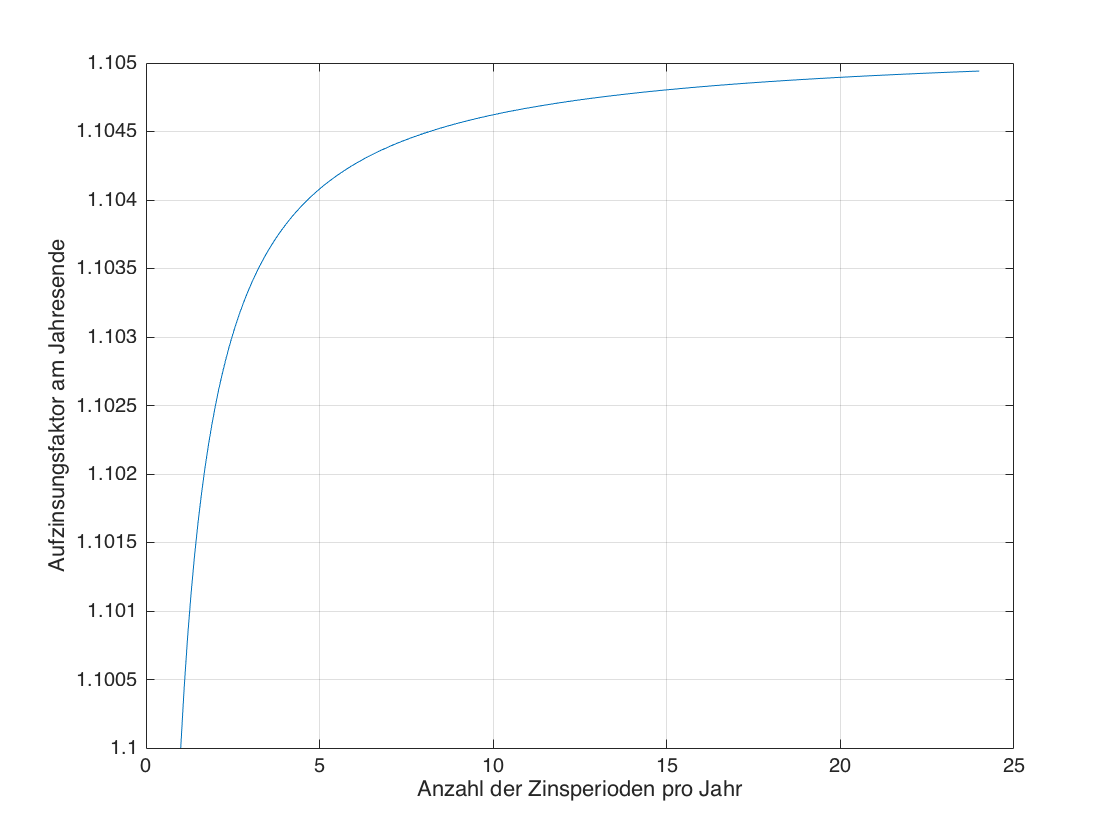
\includegraphics[width=9.5cm]{Matlab/exponentielleVerzinsung}}
\end{frame}

\begin{frame}{Effektiver Jahreszins}
\small{	\begin{bemerkung}
		Da der Endwert des Kapitals von der Anzahl der Zinsperioden (bei gleichem Zinssatz) abhängt, kann man sich fragen, was der äquivalente Zinssatz p.a. bei jährlicher Verzinsung wäre.
		
		Dazu vergleicht man den Endwert bei jährlicher Verzinsung mit einem Zinssatz $i_{\text{eff}}$ mit dem Endwert bei m-periodischer Verzinsung mit dem Zinssatz $i$:
		\begin{align*}
		K_{0} \left( 1+i_{\text{eff}} \right)^{n}  & = K_{0} \left( 1+\frac{i}{m} \right)^{n \cdot m} \\
		\Leftrightarrow i_{\text{eff}} & = \left( \left( 1+\frac{i}{m}  \right)^{m} -1 \right) 
		\end{align*}
	\end{bemerkung}
	\begin{bemerkung}
		Der \textbf{effektive Jahreszins} (auch \textbf{Rendite} genannt) $i_{\text{eff}}$ ergibt sich als Zinssatz, mit dem das Anfangskapital $K_{0}$ nachschüssig am Jahresende verzinst werden müsste, um denselben Endbetrag zu erzielen wie bei einer unterjährig m-mal mit Zinseszins verzinsten Anlageform.
	\end{bemerkung}}
\end{frame}

\begin{frame}{Effektivzins in Abhängigkeit von der Anzahl der Zinsperioden}
	\small{Bei einem Zinssatz von 10 \% ergibt sich folgende Abhängigkeit des Effektivzinses von der Anzahl der Zinsperioden im Jahr:
		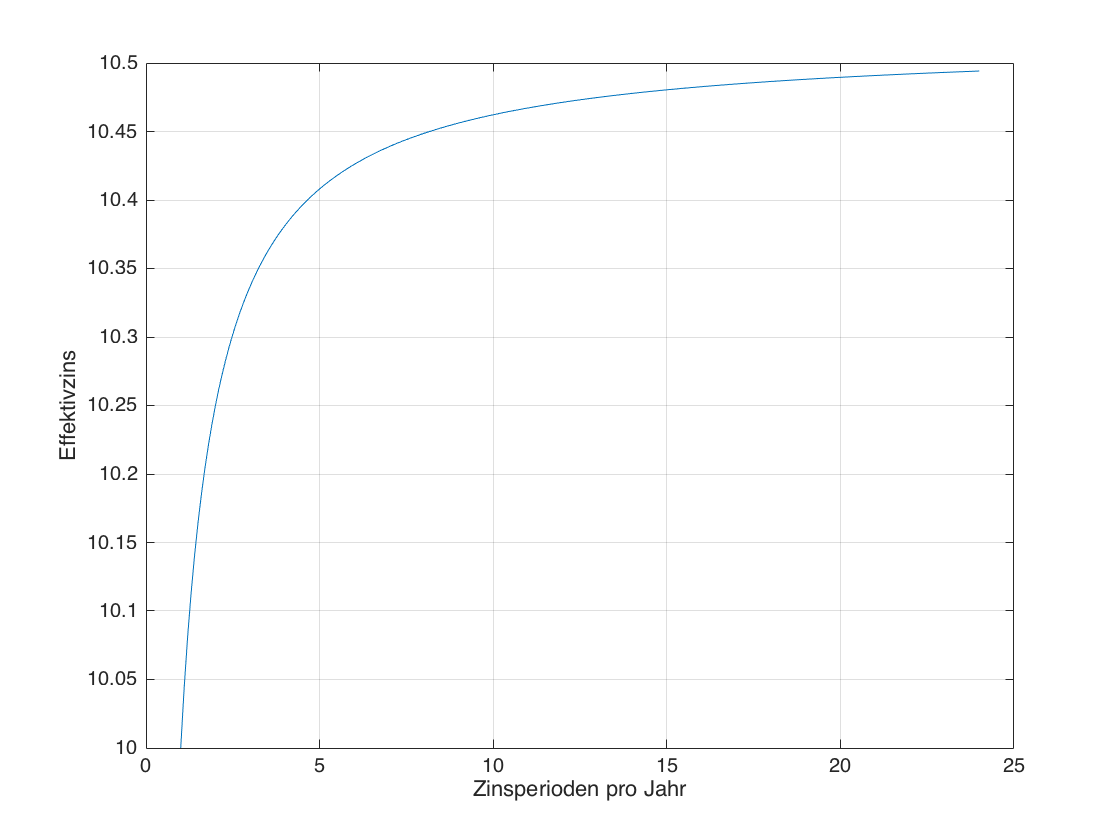
\includegraphics[width=9.5cm]{Matlab/effektivzins}		}
\end{frame}

\begin{frame}{Gemischte Verzinsung}
	\begin{bemerkung}
		Nur selten beginnt eine Anlage genau am Anfang einer Zinsperiode (z.B. bei jährlicher Verzinsung am Jahresanfang). Ebenso selten endet eine Anlage genau am Ende eines Zinsperiode (z.B. am Ende eines Jahres bei jährlicher Verzinsung),
		
		In der Regel verwendet mal also eine \textbf{gemischte Verzinsung}.
	\end{bemerkung}
	\small{\begin{example}
		Welchen Endwert hat eine Anlage von 10000 € vom 15. August 2015 zu einem Zinssatz von 12 \% am 16. März 2019?
		
		\textbf{Antwort:} Die erste Zinsperiode ist kein ganzes Jahr, sondern nur 135 Tage. Danach kommen 3 volle Jahre, danach nochmal 76 Tage, also:
		\[
		K_{\text{16. März 2019}} = \left( 1+0.12\cdot\frac{135}{360}  \right) \cdot \left( 1+0.12 \right)^{3} \cdot \left( 1+0.12\frac{76}{360} \right) \approx 15053.43
		\]
	\end{example}}
\end{frame}

\begin{frame}{Zinskurveneffekte}
\small{	\begin{bemerkung}
		Nur selten sind die Zinssätze, zu denen Geld angelegt oder geliehen werden kann, unabhängig vom Anlagezeitraum. 
		Eine \textbf{normale Zinskurve} zeigt vielmehr mit der Laufzeit der Anlage steigende Zinssätze.
		Zudem kann das Kapital im Laufe seines Anlagezeitraums unterschiedliche Zinssätze erfahren.
	\end{bemerkung}
	\begin{example}
		Ein Anfangskapital von 10000 € wird zunächst 2 Jahre lang mit 6 \% , danach 5 Jahre lang mit 7 \% und anschließend 3 Jahre lang mit 4 \% verzinst. 
		
		\textbf{Auf welchen Endwert ist das Kapital angewachsen und welchem Effektivzins entspricht die Anlage?}
		
		\textbf{Antwort:} 
		\[
		K = K_{0} \left( 1+0.06 \right)^{2} \cdot \left( 1+0.07 \right)^{5} \cdot \left( 1+0.04 \right)^{3} 
		\]
		Für den Effektivzins gilt:
		\[
		\left(1+i_{\text{eff}}\right)^{10} = \left( 1+0.06 \right)^{2} \cdot \left( 1+0.07 \right)^{5} \cdot \left( 1+0.04 \right)^{3}
 		\]
		
	\end{example}}
\end{frame}

\begin{frame}{Laufzeitberechnung}
	\begin{example}
		In welchem Zeitraum verdreitfacht sich ein Kapital bei einem Zinssatz (mit Zinseszins) von 5 \% p.a.?
		
		\textbf{Antwort:} Gesucht ist die Anzahl an Jahren $n$ in der Zinseszinsformel:
		\[
			K_{n} = 3 \cdot K_{0} = K_{0} \cdot \left( 1+0.05 \right)^{n}
		\]
		Diese Gleichung hat die Lösung
		\[
			n = \frac{\log 3}{\log 1.05} = 22,517085304
		\]
		Also verdreifacht sich das Kapital bei einem Zinssatz von 5\% in etwa 22,5 Jahren.
	\end{example}
\end{frame}

\begin{frame}{Zinseszinsformel}
{\footnotesize 	\begin{bemerkung}
		Falls man in der Zinseszinsformel mit den Aufzinsungsfaktoren rechnet, wird vieles einfacher:
		\begin{align*}
			K_{1} & = K_{0} \cdot (1+i) = K_{0} \cdot q \\
			K_{2} & = K_{1} \cdot (1+i) = K_{0} \cdot q^{2} \\
			K_{n} & = K_{0} \cdot (1+i)^{n} = K_{0} \cdot q^{n}
 		\end{align*}
 		Das gilt auch, wenn die Zinssätze verschieden sind:
		\begin{align*}
		K_{1} & = K_{0} \cdot (1+i_{1}) = K_{0} \cdot q_{1} \\
		K_{2} & = K_{1} \cdot (1+i_{2}) = K_{0} \cdot q_{1} \cdot q_{2} \\
		K_{n} & = K_{0} \cdot (1+i_{1}) \cdot (1+i_{2}) \cdot \ldots \cdot (1+i_{n}) = K_{0} \cdot q_{1} \cdot q_{2} \cdot q_{3} \cdot \ldots \cdot q_{n}
		\end{align*}
		Damit gilt für den Effektivzins:
		\begin{align*}
		K_{n} = K_{0} \underset{=: q_{\text{eff}}}{\underbrace{(1 + i_{\text{eff}})}}^{n} & = K_{0} q_{1} q_{2} \cdots q_{n} \\
		q_{\text{eff}}^{n} & = q_{1} q_{2} \cdots q_{n} \\
		q_{\text{eff}} & = \sqrt[n]{q_{1} q_{2} \cdots q_{n}}
		\end{align*}
		Der Effektivzins ist also über das \textbf{geometrische Mittel} der Aufzinsungsfaktoren zu berechnen.
	\end{bemerkung}
}\end{frame}

\begin{frame}{Beispiel - Rendite}
{\small 	\begin{example}
		Sie kaufen Bundesschatzbriefe vom Typ B (mit Zinseszins) im Nennwert von 10000 €, die folgende Verzinsung versprechen: 3.5 \% im 1. Jahr, 3.75 \% im 2. Jahr, 4 \% im 3. Jahr, 4.5 \% im 4. Jahr, 5 \% im 5. Jahr, 5.5 \% im 6. Jahr 6.5 \% im 7. Jahr.
		
		Welche Endsumme und welche Rendite erzielt diese Anlage, wenn man das Wertpapier über die vollen sieben Jahr hält?
		
		\textbf{Antwort:} Der Endwert berechnet sich
		\begin{align*}
		K_{7} & = K_{0} \cdot q_{1} \cdot q_{2} \cdots q_{7} \\ 
		& = 10000 \cdot 1.035 \cdot 1.0375 \cdot 1.04 \cdot 1.045 \cdot 1.05 \cdot 1.055 \cdot 1.065 \\ 
		& = 13767.96 \text{€}  
		\end{align*}
		Für den Effektivzins gilt:
		\begin{align*}
		\left( 1+ i_{\text{eff}} \right)^{7} & = q_{\text{eff}}^{7} & = 1.035 \cdot 1.0375 \cdot 1.04 \cdot 1.045 \cdot 1.05 \cdot 1.055 \cdot 1.065 \\
		\Leftrightarrow \left( 1 + i_{\text{eff}} \right) & = q_{\text{eff}} & = \sqrt[7]{1.035 \cdot 1.0375 \cdot 1.04 \cdot 1.045 \cdot 1.05 \cdot 1.055 \cdot 1.065}  \\
		\Leftrightarrow i_{\text{eff}} & & = q_{\text{eff}} - 1  = \sqrt[7]{1.376795543} -1 = 0.046739211
		\end{align*}
	\end{example}
}\end{frame}

\subsection{Rentenrechnung}
\begin{frame}{Rentenrechnung}
	\begin{definition}
		
	\end{definition}
\end{frame}

\begin{frame}{Endwert einer nachschüssigen Rente}
	\textbf{Frage}: Welchen Wert hat eine Rente mit der nachschüssigen (N) Rentenrate $R$, die über $n$ Jahre gezahlt wird, am Ende der Laufzeit?
	
	\footnotesize{
	\textbf{Antwort}: \begin{tabular}{|c|c|c|c|}
		\hline Jahr & nachschüssige Rate & verbleibender Zeitraum & Endwert der Rate \\ 
		\hline $1$ & $R$ & $n-1$ & $Rq^{n-1}$ \\ 
		\hline $2$ & $R$ & $n-2$ & $Rq^{n-2}$ \\ 
		\hline $3$ & $R$ & $n-3$ & $Rq^{n-3}$ \\ 
		\hline \vdots & \vdots & \vdots & \vdots \\ 
		\hline $n-2$ & $R$ & $2$ & $Rq^{2}$ \\ 
		\hline $n-1$ & $R$ & $1$ & $Rq$ \\ 
		\hline $n$ & $R$ & $0$ & $R$ \\ 
		\hline 
	\end{tabular}
	
	Damit ist
	\[
	R_{n}^{N} = R + Rq + Rq^{2} + R q^{3} + \ldots + Rq^{n-1} = \sum\limits_{i=1}^{n} Rq^{i-1} = R \sum\limits_{i=1}^{n} q^{i-1} = R \frac{q^{n}-1}{q-1}
	\] }
\end{frame}

\begin{frame}{Barwert einer nachschüssigen Rente}
	\textbf{Frage}: Welchen Barwert hat eine Rente mit der nachschüssigen (N) Rentenrate $R$, die über $n$ Jahre gezahlt wird, heute?
	
	\footnotesize{
		\textbf{Antwort}: \begin{tabular}{|c|c|c|c|}
			\hline Jahr & nachschüssige Rate & verbleibender Zeitraum & Barwert der Rate \\ 
			\hline $1$ & $R$ & $n-1$ & $\frac{R}{q}$ \\ 
			\hline $2$ & $R$ & $n-2$ & $\frac{R}{q^{2}}$ \\ 
			\hline $3$ & $R$ & $n-3$ & $\frac{R}{q^{3}}$ \\ 
			\hline \vdots & \vdots & \vdots & \vdots \\ 
			\hline $n-2$ & $R$ & $2$ & $\frac{R}{q^{n-2}}$ \\ 
			\hline $n-1$ & $R$ & $1$ & $\frac{R}{q^{n-1}}$ \\ 
			\hline $n$ & $R$ & $0$ & $\frac{R}{q^{n}}$ \\ 
			\hline 
		\end{tabular}
		
		Damit ist
		\[
		B_{n}^{N} = \frac{R}{q} + \frac{R}{q^{2}} + \frac{R}{q^{3}} + \ldots + \frac{R}{q^{n}} = \frac{R}{q^{n}} \left( q^{n-1} + q^{n-2} + \ldots + q + 1 \right) = R \cdot \frac{1}{q^{n}} \cdot \frac{q^n-1}{q-1}
		\]
	}
\end{frame}

\begin{frame}{Endwert einer vorschüssigen Rente}
	\textbf{Frage}: Welchen Wert hat eine Rente mit der vorschüssigen (V) Rentenrate $R$, die über $n$ Jahre gezahlt wird, am Ende der Laufzeit?
	
	\footnotesize{
		\textbf{Antwort}: \begin{tabular}{|c|c|c|c|}
			\hline Jahr & vorschüssige Rate & verbleibender Zeitraum & Endwert der Rate \\ 
			\hline $1$ & $R$ & $n$ & $Rq^{n}$ \\ 
			\hline $2$ & $R$ & $n-1$ & $Rq^{n-1}$ \\ 
			\hline $3$ & $R$ & $n-2$ & $Rq^{n-2}$ \\ 
			\hline \vdots & \vdots & \vdots & \vdots \\ 
			\hline $n-2$ & $R$ & $3$ & $Rq^{3}$ \\ 
			\hline $n-1$ & $R$ & $2$ & $Rq^{2}$ \\ 
			\hline $n$ & $R$ & $1$ & $Rq$ \\ 
			\hline 
		\end{tabular}
		
		Damit ist
		\[
		R_{n}^{V} = Rq + Rq^{2} + Rq^{3} + R q^{4} + \ldots + Rq^{n} = \sum\limits_{i=1}^{n} Rq^{i} = Rq \sum\limits_{i=1}^{n} q^{i-1} = Rq \frac{q^{n}-1}{q-1}
		\] }
\end{frame}

\begin{frame}{Barwert einer vorschüssigen Rente}
	\textbf{Frage}: Welchen Barwert hat eine Rente mit der vorschüssigen (V) Rentenrate $R$, die über $n$ Jahre gezahlt wird, heute?
	
	\footnotesize{
		\textbf{Antwort}: \begin{tabular}{|c|c|c|c|}
			\hline Jahr & vorschüssige Rate & verbleibender Zeitraum & Barwert der Rate \\ 
			\hline $1$ & $R$ & $n-1$ & $R$ \\ 
			\hline $2$ & $R$ & $n-2$ & $\frac{R}{q}$ \\ 
			\hline $3$ & $R$ & $n-3$ & $\frac{R}{q^{2}}$ \\ 
			\hline \vdots & \vdots & \vdots & \vdots \\ 
			\hline $n-2$ & $R$ & $2$ & $\frac{R}{q^{n-3}}$ \\ 
			\hline $n-1$ & $R$ & $1$ & $\frac{R}{q^{n-2}}$ \\ 
			\hline $n$ & $R$ & $0$ & $\frac{R}{q^{n-1}}$ \\ 
			\hline 
		\end{tabular}
		
		Damit ist
		\begin{align*}
		B_{n}^{V} = R + \frac{R}{q} + \frac{R}{q^{2}} + \frac{R}{q^{3}} + \ldots + \frac{R}{q^{n-1}} & = \frac{R}{q^{n-1}} \left( q^{n-1} + q^{n-2} + \ldots + q + 1 \right) \\  & = R \cdot \frac{1}{q^{n}} \cdot q \frac{q^{n}-1}{q-1}
		\end{align*}}
\end{frame}

\begin{frame}{Zusammenfassung der zentralen Rentenformeln}
	\begin{tabular}{|c||c|c|}
			\hline End-/Barwert & Rate vorschüssig & Rate nachschüssig \\ \hline
			\hline Barwert& $Rq\frac{1}{q^n}\frac{q^n -1}{q-1}$ & $R\frac{1}{q^n}\frac{q^n -1}{q-1}$ \\ 
			\hline Endwert & $Rq\frac{q^n -1}{q-1}$ & $R\frac{q^n -1}{q-1}$ \\ 
			\hline 
		\end{tabular}
\end{frame}

%\part{Mathematik II}

%\begin{frame}{Hinweis}
%	Diese Folien sind nicht vollständig und werden noch immer verändert und erweitert!
%\end{frame}

\section*{Organisatorisches}
\begin{frame}{Kontaktdaten}
	\begin{itemize}
		\item Prof. Dr. Stefan Böcker, FRM
		\begin{itemize}
			\item Raum: H.120
			\item Telefon: +49 2331 9330-6707
			\item Email: \href{mailto:boecker.stefan@fh-swf.de}{boecker.stefan@fh-swf.de}
			\item Vorlesung%, Übung am Donnerstag morgens
			\item Sprechstunde: nach Vereinbarung per Email
%			\item Aktuelle Informationen und Link zu diesen Folien: \href{https://lmt.fh-swf.de/de/mathematik2}{https://lmt.fh-swf.de/de/mathematik2}
		\end{itemize}
		\item Dipl.-Math. Silke Beckmann
		\begin{itemize}
			\item Raum: H.101
			\item Telefon: +49 2331 9330-6791
			\item Email: \href{mailto:beckmann.silke@fh-swf.de}{beckmann.silke@fh-swf.de}
			\item Alle Übungen
		\end{itemize}
		\item Moodle
			Alle Informationen zur Mathematik 1 finden Sie im zugehörigen Moodle-Kurs:
			\href{https://elearning.fh-swf.de/course/view.php?id=7719}{Mathematik 2 in Moodle}
%		\item Tutoren
%			\begin{itemize}
%				\item Morgane Woeffler \href{mailto:woeffler.morgane@fh-swf.de}{woeffler.morgane@fh-swf.de}
%				\item Thomas Schulte \href{mailto:schulte.thomas@fh-swf.de}{schulte.thomas@fh-swf.de}
%			\end{itemize}		
	\end{itemize}
\end{frame}

\begin{frame}{Literatur}
\footnotesize{Bei der Vorbereitung dieser Vorlesung habe ich mich sehr an dem Buch von Knorrenschild \cite{knorr-mathe} orientiert. Parallel zur Vorlesung eignen sich aber auch die Bücher von Dietlein und Romberg \cite{diet-panik} und Walz \cite{walz-mathe} vor Nachbearbeitung des Stoffes.

Mein persönlicher Favorit ist das Buch von Arens et al.\cite{arens-mathe}.

Für die Finanzmathematik ist das Buch von Bernd Luderer sehr elementar, dafür aber auch sehr gut (fast) ohne jede Vorkenntnisse zu verstehen: \cite{luderer-starthilfe}

\printbibliography
}
\end{frame}

\begin{frame}{Software}
	Für die Erstellung der meisten Grafiken und Animationen habe ich folgende Software benutzt:
	\begin{itemize}
		\item Geogebra - Mathematik-Software, speziell für Geometrie
		
		\href{https://www.geogebra.org/}{https://www.geogebra.org/}
		\item MATLAB\textsuperscript{\textregistered} - Software von MathWorks\textsuperscript{\textregistered}
		
		\href{http://www4.fh-swf.de/de/home/studierende/its/software/matlab__campuslizenz_/matlab_campuslizenz.php}{Campus-Lizenz für MATLAB\textsuperscript{\textregistered}}
	\end{itemize}
\end{frame}

\begin{frame}{Inhaltsübersicht}
\tableofcontents
\end{frame}

%\section{Funktionen und deren Eigenschaften}
\subsection{Elementare Eigenschaften von Funktionen}
\subsubsection{Nullstellen}
\begin{frame}{Nullstellen}
	\begin{definition}
		Die Funktion $y=f(x)$ besitzt an der Stelle $x_{0}$ eine \textbf{Nullstelle}, wenn
		\[
			f(x_{0}) = 0
		\]
		ist.
	\end{definition}
\begin{bemerkung}
			In der Nullstelle $x_{0}$ berührt oder schneidet der Funktionsgraph die x-Achse.
\end{bemerkung}

\end{frame}
\begin{frame}{Nullstelle einer linearen Funktion}
\begin{example}
	Die lineare Funktion $y = x - 2$ hat eine Nullstelle bei $x_{0}= 2$ und schneidet die x-Achse.
	\definecolor{qqwuqq}{rgb}{0.,0.39215686274509803,0.}
	\definecolor{qqwuqq}{rgb}{0.,0.39215686274509803,0.}
	\begin{tikzpicture}[line cap=round,line join=round,>=triangle 45,x=0.5cm,y=0.4cm]
	\draw[->,color=black] (-4.3,0.) -- (14.62,0.);
	\foreach \x in {-4.,-3.,-2.,-1.,1.,2.,3.,4.,5.,6.,7.,8.,9.,10.,11.,12.,13.,14.}
	\draw[shift={(\x,0)},color=black] (0pt,2pt) -- (0pt,-2pt) node[below] {\footnotesize $\x$};
	\draw[->,color=black] (0.,-7.36) -- (0.,6.3);
	\foreach \y in {-7.,-6.,-5.,-4.,-3.,-2.,-1.,1.,2.,3.,4.,5.,6.}
	\draw[shift={(0,\y)},color=black] (2pt,0pt) -- (-2pt,0pt) node[left] {\footnotesize $\y$};
	\draw[color=black] (0pt,-10pt) node[right] {\footnotesize $0$};
	\clip(-4.3,-7.36) rectangle (14.62,6.3);
	\draw[line width=1.2pt,color=qqwuqq,smooth,samples=100,domain=-4.300000000000001:14.620000000000005] plot(\x,{(\x)-2.0});
	\begin{scriptsize}
	\draw[color=qqwuqq] (-4.14,-6.28) node {$f$};
	\end{scriptsize}
	\end{tikzpicture}
	\end{example}
\end{frame}

\begin{frame}{Nullstelle einer quadratischen Funktion}
	\begin{example}
		Die quadratische Funktion 
		\[
			f(x)=(x-1)^2
		\]
		besitzt eine Nullstelle bei $x=1$ und berührt dort die x-Achse.
		\definecolor{ccqqqq}{rgb}{0.8,0.,0.}
		\begin{tikzpicture}[line cap=round,line join=round,>=triangle 45,x=0.5cm,y=0.25cm]
		\draw[->,color=black] (-4.3,0.) -- (14.62,0.);
		\foreach \x in {-4.,-3.,-2.,-1.,1.,2.,3.,4.,5.,6.,7.,8.,9.,10.,11.,12.,13.,14.}
		\draw[shift={(\x,0)},color=black] (0pt,2pt) -- (0pt,-2pt) node[below] {\footnotesize $\x$};
		\draw[->,color=black] (0.,-7.36) -- (0.,6.3);
		\foreach \y in {-7.,-6.,-5.,-4.,-3.,-2.,-1.,1.,2.,3.,4.,5.,6.}
		\draw[shift={(0,\y)},color=black] (2pt,0pt) -- (-2pt,0pt) node[left] {\footnotesize $\y$};
		\draw[color=black] (0pt,-10pt) node[right] {\footnotesize $0$};
		\clip(-4.3,-7.36) rectangle (14.62,6.3);
		\draw[line width=1.2pt,color=ccqqqq,smooth,samples=100,domain=-4.300000000000001:14.620000000000005] plot(\x,{((\x)-1.0)^(2.0)});
		\begin{scriptsize}
		\draw[color=ccqqqq] (-1.24,6.14) node {$f$};
		\end{scriptsize}
		\end{tikzpicture}
		Diese Nullstelle wird auch als \textbf{doppelte Nullstelle} bezeichnet, weil zwei Terme $x-1$ und $x-1$ gleichzeitig null werden.
	\end{example}
\end{frame}

\begin{frame}{Nullstellen periodischer Funktionen}
	\begin{example}
		Die Funktion $f(x)=\sin(x)$ hat unendlich viele Nullstellen. Die Nullstellen sind an den Stellen $x_{i} = i \pi$ für $i \in \mathbb{Z}$.
		\definecolor{qqqqff}{rgb}{0.,0.,1.}
		\begin{tikzpicture}[line cap=round,line join=round,>=triangle 45,x=0.5cm,y=0.9cm]
		\draw[->,color=black] (-4.28,0.) -- (14.6,0.);
		\foreach \x in {-4.,-3.,-2.,-1.,1.,2.,3.,4.,5.,6.,7.,8.,9.,10.,11.,12.,13.,14.}
		\draw[shift={(\x,0)},color=black] (0pt,2pt) -- (0pt,-2pt) node[below] {\footnotesize $\x$};
		\draw[->,color=black] (0.,-3.22) -- (0.,2.98);
		\foreach \y in {-3.,-2.5,-2.,-1.5,-1.,-0.5,0.5,1.,1.5,2.,2.5}
		\draw[shift={(0,\y)},color=black] (2pt,0pt) -- (-2pt,0pt) node[left] {\footnotesize $\y$};
		\draw[color=black] (0pt,-10pt) node[right] {\footnotesize $0$};
		\clip(-4.28,-3.22) rectangle (14.6,2.98);
		\draw[line width=1.2pt,color=qqqqff,smooth,samples=100,domain=-4.280000000000001:14.600000000000003] plot(\x,{sin(((\x))*180/pi)});
		\begin{scriptsize}
		\draw[color=qqqqff] (-4.120338266384779,0.7741434846266446) node {$h$};
		\end{scriptsize}
		\end{tikzpicture}
	\end{example}
\end{frame}

\subsubsection{Symmetrie}
\begin{frame}{Symmetrie}
	\begin{definition}
		Eine Funktion f heißt \textbf{gerade} bzw. \textbf{achsensymmetrisch}, wenn  die Bedingung
		\[
			f(x) = f(-x) \qquad \forall x \in D
		\]
		erfüllt ist.
	\end{definition}
	\begin{bemerkung}
		Streng genommen nennt man nur die Funktion \textbf{gerade}, der dazugehörige Funktionsgraph ist dann \textbf{achsensymmetrisch} (zur y-Achse).
		
		$D$ bezeichnet den Definitionsbereich der Funktion, das heißt: $D$ ist die Menge der Zahlen $x$, für die $f(x)$ überhaupt definiert ist.
		
		$\forall$ ist das Symbol für "{}für alle"{}.
	\end{bemerkung}
\end{frame}

\begin{frame}{Symmetrie einer quadratischen Funktion}
	\begin{example}
		Die Funktion $f(x)=x^2$ ist gerade\footnote{Das liegt auch daran, dass nur (ein) gerade(r) Exponent(en) vorkommen!}. 
		\definecolor{ffvvqq}{rgb}{1.,0.3333333333333333,0.}
		\begin{tikzpicture}[line cap=round,line join=round,>=triangle 45,x=2cm,y=1.5cm]
		\draw[->,color=black] (-2.1844397463002125,0.) -- (2.246173361522198,0.);
		\foreach \x in {-2.,-1.8,-1.6,-1.4,-1.2,-1.,-0.8,-0.6,-0.4,-0.2,0.2,0.4,0.6,0.8,1.,1.2,1.4,1.6,1.8,2.,2.2}
		\draw[shift={(\x,0)},color=black] (0pt,2pt) -- (0pt,-2pt) node[below] {\footnotesize $\x$};
		\draw[->,color=black] (0.,-0.21531478770132104) -- (0.,2.9618448023426045);
		\foreach \y in {-0.2,0.2,0.4,0.6,0.8,1.,1.2,1.4,1.6,1.8,2.,2.2,2.4,2.6,2.8}
		\draw[shift={(0,\y)},color=black] (2pt,0pt) -- (-2pt,0pt) node[left] {\footnotesize $\y$};
		\draw[color=black] (0pt,-10pt) node[right] {\footnotesize $0$};
		\clip(-2.1844397463002125,-0.21531478770132104) rectangle (2.246173361522198,2.9618448023426045);
		\draw[line width=1.2pt,color=ffvvqq,smooth,samples=100,domain=-2.1844397463002125:2.246173361522198] plot(\x,{(\x)^(2.0)});
		\begin{scriptsize}
		\draw[color=ffvvqq] (-1.6598851288836058,2.9292824053729007) node {$f$};
		\end{scriptsize}
		\end{tikzpicture}
	\end{example}
\end{frame}

\begin{frame}{Symmetrie der Kosinus-Funktion}
	\begin{example}
		Die Funktion $f(x)=\cos x$ ist gerade.
		\definecolor{zzttff}{rgb}{0.6,0.2,1.}
		\begin{tikzpicture}[line cap=round,line join=round,>=triangle 45,x=0.45cm,y=1.0cm]
		\draw[->,color=black] (-10.897842255586003,0.) -- (11.532136602764956,0.);
		\foreach \x in {-10.,-8.,-6.,-4.,-2.,2.,4.,6.,8.,10.}
		\draw[shift={(\x,0)},color=black] (0pt,2pt) -- (0pt,-2pt) node[below] {\footnotesize $\x$};
		\draw[->,color=black] (0.,-2.4276582084565703) -- (0.,1.9494486572603942);
		\foreach \y in {-2.,-1.5,-1.,-0.5,0.5,1.,1.5}
		\draw[shift={(0,\y)},color=black] (2pt,0pt) -- (-2pt,0pt) node[left] {\footnotesize $\y$};
		\draw[color=black] (0pt,-10pt) node[right] {\footnotesize $0$};
		\clip(-10.897842255586003,-2.4276582084565703) rectangle (11.532136602764956,1.9494486572603942);
		\draw[line width=1.2pt,color=zzttff,smooth,samples=100,domain=-10.897842255586003:11.532136602764956] plot(\x,{cos(((\x))*180/pi)});
		\begin{scriptsize}
		\draw[color=zzttff] (-10.708159559109461,-0.18463126409209377) node {$cos$};
		\end{scriptsize}
		\end{tikzpicture}
		
	\end{example}
\end{frame}

\begin{frame}{Symmetrie}
	\begin{definition}
		Eine Funktion f heißt \textbf{ungerade} bzw. \textbf{punktsymmetrisch}, wenn  die Bedingung
		\[
		f(x) = - f(-x) \qquad \forall x \in D
		\]
		erfüllt ist.
	\end{definition}
	\begin{bemerkung}
		Streng genommen nennt man wieder nur die Funktion \textbf{ungerade}, der dazugehörige Funktionsgraph ist dann \textbf{punktsymmetrisch} (zum Ursprung).
	\end{bemerkung}
\end{frame}

\begin{frame}{Symmetrie einer kubischen Funktion}
	\begin{example}
		Die Funktion $f(x)=x^3$ ist ungerade\footnote{Das liegt auch daran, dass nur (ein) ungerade(r) Exponent(en) vorkommen!}.
		\begin{tikzpicture}[line cap=round,line join=round,>=triangle 45,x=3.5cm,y=8.0cm]
		\draw[->,color=black] (-1.4479556964005578,0.) -- (1.5057863754810505,0.);
		\foreach \x in {-1.4,-1.2,-1.,-0.8,-0.6,-0.4,-0.2,0.2,0.4,0.6,0.8,1.,1.2,1.4}
		\draw[shift={(\x,0)},color=black] (0pt,2pt) -- (0pt,-2pt) node[below] {\footnotesize $\x$};
		\draw[->,color=black] (0.,-0.3408915185936749) -- (0.,0.23551761598633617);
		\foreach \y in {-0.3,-0.25,-0.2,-0.15,-0.1,0.15,0.2}
		\draw[shift={(0,\y)},color=black] (2pt,0pt) -- (-2pt,0pt) node[left] {\footnotesize $\y$};
		\draw[color=black] (0pt,-10pt) node[right] {\footnotesize $0$};
		\clip(-1.4479556964005578,-0.3408915185936749) rectangle (1.5057863754810505,0.23551761598633617);
		\draw[line width=1.2pt,smooth,samples=100,domain=-1.4479556964005578:1.5057863754810505] plot(\x,{(\x)^(3.0)});
		\begin{scriptsize}
		\draw[color=black] (-0.6580014213624532,-0.3299203344801462) node {$x^3$};
		\end{scriptsize}
		\end{tikzpicture}
		 
	\end{example}
\end{frame}

\begin{frame}{Symmetrie der Sinus-Funktion}
	\begin{example}
		Die Funktion $f(x)=\sin x$ ist ungerade.
		\definecolor{zzttff}{rgb}{0.6,0.2,1.}
		\begin{tikzpicture}[line cap=round,line join=round,>=triangle 45,x=0.45cm,y=1.0cm]
		\draw[->,color=black] (-10.897842255586003,0.) -- (11.532136602764956,0.);
		\foreach \x in {-10.,-8.,-6.,-4.,-2.,2.,4.,6.,8.,10.}
		\draw[shift={(\x,0)},color=black] (0pt,2pt) -- (0pt,-2pt) node[below] {\footnotesize $\x$};
		\draw[->,color=black] (0.,-2.4276582084565703) -- (0.,1.9494486572603942);
		\foreach \y in {-2.,-1.5,-1.,-0.5,0.5,1.,1.5}
		\draw[shift={(0,\y)},color=black] (2pt,0pt) -- (-2pt,0pt) node[left] {\footnotesize $\y$};
		\draw[color=black] (0pt,-10pt) node[right] {\footnotesize $0$};
		\clip(-10.897842255586003,-2.4276582084565703) rectangle (11.532136602764956,1.9494486572603942);
		\draw[line width=1.2pt,color=zzttff,smooth,samples=100,domain=-10.897842255586003:11.532136602764956] plot(\x,{sin(((\x))*180/pi)});
		\begin{scriptsize}
		\draw[color=zzttff] (-10.708159559109461,-0.18463126409209377) node {$sin$};
		\end{scriptsize}
		\end{tikzpicture}
		
	\end{example}
\end{frame}


\subsubsection{Monotonie}
\begin{frame}{Monotonie}
	\begin{definition}
		Eine Funktion $y=f(x)$ heißt
		\begin{itemize}
			\item \textbf{monoton wachsend}, wenn $\forall  x_{1}, x_{2} \in D(f) \mbox{ mit } x_{1} < x_{2}  \qquad f(x_{1}) \leq f(x_{2})$ gilt
			\item \textbf{streng monoton wachsend}, wenn $\forall  x_{1}, x_{2} \in D(f) \mbox{ mit } x_{1} < x_{2}  \qquad f(x_{1}) < f(x_{2})$ gilt
			\item \textbf{monoton fallend}, wenn $\forall  x_{1}, x_{2} \in D(f) \mbox{ mit } x_{1} < x_{2}  \qquad f(x_{1}) \geq f(x_{2})$ gilt
			\item \textbf{streng monoton fallend}, wenn $\forall  x_{1}, x_{2} \in D(f) \mbox{ mit } x_{1} < x_{2}  \qquad f(x_{1}) > f(x_{2})$ gilt
						
		\end{itemize}
	\end{definition}
\end{frame}

\begin{frame}{Beispiele - Monotonie}
	\begin{example}
		\begin{itemize}
			\item Jede lineare Funktion $y = a x + b$ mit $a>0$ ist streng monoton wachsend.
			\item Jede lineare Funktion $y = a x + b$ mit $a<0$ ist streng monoton fallend.
			\item Die kubische Funktion $y=x^3$ ist streng monoton wachsend.
			\item Die Exponentialfunktion $y=e^{x}$ ist streng monoton wachsend.
			\item Die Exponentialfunktion $y=e^{-x}$ ist streng monoton fallend.
		\end{itemize}
	\end{example}
\end{frame}

\begin{frame}{Bemerkung zur Monotonie}
	\begin{bemerkung}
		Falls die Funktion $y=f(x)$
		\begin{itemize}
			\item streng monoton wachsend ist, gilt $\frac{f(x_{2}) - f(x_{1})}{x_{2} - x_{1}} > 0$ 
			\item streng monoton fallend ist, gilt
			$\frac{f(x_{2}) - f(x_{1})}{x_{2} - x_{1}} < 0$
			\item monoton wachsend ist, gilt
			$\frac{f(x_{2}) - f(x_{1})}{x_{2} - x_{1}} \geq 0$ 
			\item monoton fallend ist, gilt
			$\frac{f(x_{2}) - f(x_{1})}{x_{2} - x_{1}} \leq 0$ 
		\end{itemize}
		$\forall x_{1} \neq x_{2} \in D(f)$.
	\end{bemerkung}
\end{frame}

\subsubsection{Periodizität}
\begin{frame}{Periodizität}
	\begin{definition}
		Eine Funktion $y=f(x)$ heißt periodisch mit der Periode $T$, wenn für alle $x \in D(f)$ und für alle $n \in \mathbb{Z}$ sowohl
		\begin{itemize}
			\item $x+n \cdot T \in D(f)$ ist als auch
			\item $f(x+n \cdot T) = f(x)$ gilt.   
		\end{itemize} 
	\end{definition}
	\begin{example}
		Die Funktion $y = \sin(x)$ ist periodisch mit der Periode $T=2 \pi$, denn
		\[
			\sin(x) = \sin( x + n \cdot 2 \pi) \qquad \forall n\in \mathbb{Z}, x \in  \mathbb{R}
		\]
	\end{example}
\end{frame}

\subsection{Grenzwerte von Funktionen}
\subsubsection{Grenzwerte für $x \to x_{0}$}
\begin{frame}{Grenzwerte für $x \to x_{0}$}
	\begin{definition}
		Eine Funktion $y = f(x)$ sei in einer Umgebung von $x_{0} \in \mathbb{R}$ definiert\footnote{D.h. anschaulich, dass jeder Punkt $x$, der nach genug an $x_{0}$ liegt, im Definitionsbereich der Funktion liegt.}. Wenn für jede beliebige Folge $(x_{n})$ mit $\lim_{n \to \infty}x_{n} = x_{0}$ gilt:
	\[
		\lim_{n \to \infty} f(x_{n}) = g
	\]
	so heißt $g$ der Grenzwert der Funktion $f$ an der Stelle $x_{0}$ und man schreibt:
	\[
		\lim_{x \to x_{0}} f(x) = g
	\]
	\end{definition}
\end{frame}	

\begin{frame}{Grenzwerte einer Funktion für $x \to x_{0}$}
	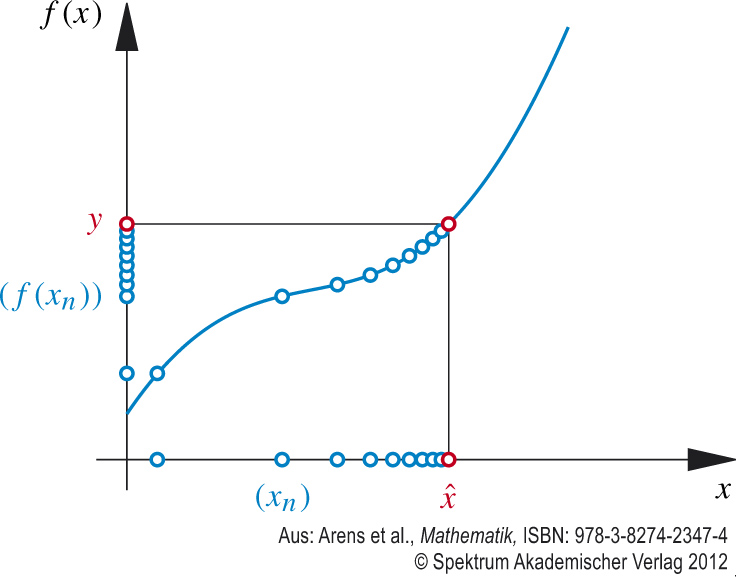
\includegraphics[width=10cm]{stetigkeit.jpg}
\end{frame}
\begin{frame}{Grenzwerte einer Funktion für $x \to x_{0}$}
	\begin{bemerkung}
		\begin{itemize}
			\item Der Punkt $x_{0}$ muss dabei nicht unbedingt im Definitionsbereich der Funktion liegen.
			\item Man unterscheidet manchmal (siehe nächste Folie) noch, ob der Grenzwert nur für $x < x_{0}$ bzw. $x > x_{0}$ betrachtet wird. Die Definition hier verlangt noch, dass es für \textbf{jede} Folge gilt.
		\end{itemize}
	\end{bemerkung}
\end{frame}

\begin{frame}{Grenzwerte einer Funktion für $x \to x_{0}$}
	\begin{definition}
		Beschränkt man die Folge $x_{n}$ in der Definition des Grenzwertes (s.o.) auf Folgen mit $x_{n}<x_{0}$ und existiert dieser Grenzwert, so nennt man diesen den \textbf{linksseitigen Grenzwert} von $f$ an der Stelle $x_{0}$ und schreibt:
		\[
			\lim_{x \nearrow x_{0}} f(x) = \lim_{x \to x_{0} - 0} f(x) = g_{l}
		\]
	\end{definition}
		\begin{definition}
			Beschränkt man die Folge $x_{n}$ in der Definition des Grenzwertes (s.o.) auf Folgen mit $x_{n}>x_{0}$ und existiert dieser Grenzwert, so nennt man diesen den \textbf{rechtsseitigen Grenzwert} von $f$ an der Stelle $x_{0}$ und schreibt:
			\[
			\lim_{x \searrow x_{0}} f(x) =\lim_{x \to x_{0} + 0} f(x) = g_{r}
			\]
		\end{definition}
\end{frame}
\begin{frame}{Zusammenhang der Grenzwertbegriffe}
	\begin{bemerkung}
		Offenbar existiert der Grenzwert einer Funktion $f$ an der Stelle $x_{0}$ genau dann, wenn sowohl der rechtsseitige als auch der linksseitige Grenzwert existieren und die beiden übereinstimmen. Dann ist
		\[
			\lim_{x \to x_{0}} f(x) = \lim_{x \nearrow x_{0}} f(x) = \lim_{x \searrow x_{0}} f(x)
		\]
	\end{bemerkung}
\end{frame}

\begin{frame}{Grenzwerte einer Funktion für $x \to x_{0}$}
	Für die Funktion
	\[
	f(x)=\begin{cases}
	0 & \text{ falls } x \leq 0 \\
	\sin(\frac{1}{x}) & \text{ falls } x>0
	\end{cases}
	\]
	existiert der rechtsseitige Grenzwert nicht!
	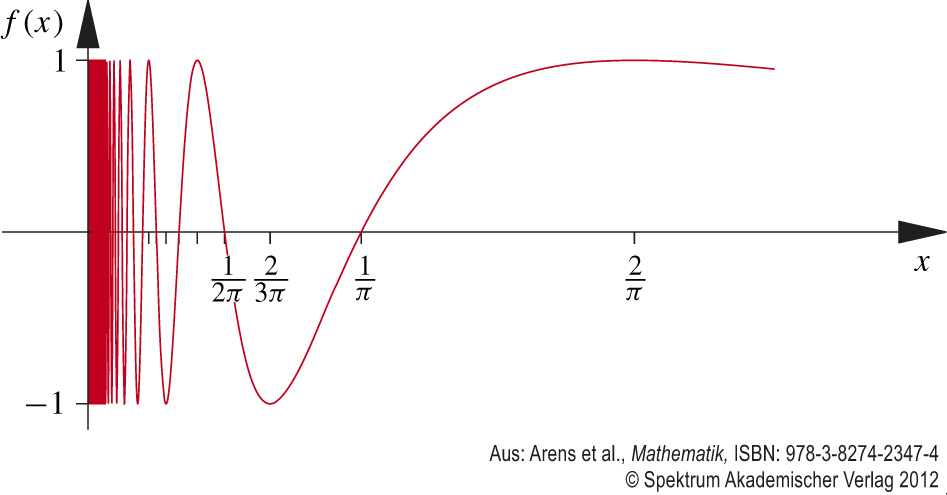
\includegraphics[width=9cm]{unstetig.jpg}
\end{frame}

\subsubsection{Grenzwerte für $x \to \pm \infty$}
\begin{frame}{Grenzwerte für $x \to \pm \infty$}
	\begin{definition}
		Für eine Funktion $y=f(x)$ definiert man
		\[
		\lim_{x \to \infty} f(x) = g \in \mathbb{R}
		\]
		wenn für alle Folgen $(x_{n})$ mit $x_{n} \to \infty$ der Grenzwert der Folge $f(x_{n})$ existiert und unabhängig von der Wahl der Folge gleich $g$ ist.
	\end{definition}
		\begin{definition}
			Für eine Funktion $y=f(x)$ definiert man
			\[
			\lim_{x \to -\infty} f(x) = g \in \mathbb{R}
			\]
			wenn für alle Folgen $(x_{n})$ mit $x_{n} \to -\infty$ der Grenzwert der Folge $f(x_{n})$ existiert und unabhängig von der Wahl der Folge gleich $g$ ist.
		\end{definition}	
\end{frame}

\subsection{Stetigkeit von Funktionen}
\begin{frame}{Stetigkeit}
	\begin{definition}
		Eine Funktion $f$ heißt \textbf{stetig an der Stelle $x_{0}$}, wenn sowohl der rechtsseitige als auch der linksseitige Grenzwert der Funktion an der Stelle $x_{0}$ existiert, beide gleich sind und der gemeinsame Grenzwert gleich $f(x_{0})$ ist, also:
		\[
			\lim_{x \to x_{0}} f(x) = \lim_{x \searrow x_{0}} f(x) = \lim_{x \nearrow x_{0}} f(x) = f(x_{0})
		\]
		ist.
		Stellen, an denen eine Funktion nicht stetig ist, nennt man \textbf{Unstetigkeitsstellen}.
	\end{definition}
\end{frame}	
\begin{frame}{Stetigkeit von Funktionen}
	\begin{theorem}
		Seien $f$ und $g$ in $x_{0}$ stetig und $c \in \mathbb{R}$ eine Konstante. Dann gilt:
		\begin{itemize}
			\item $f + g$, $f \cdot g$ und $c \cdot f$ sind stetig in $x_{0}$.
			\item Falls $g(x_{0}) \neq 0$, so ist auch $\frac{f}{g}$ stetig in $x_{0}$.
			\item $f^{r}$, d.h. die Funktion $x \mapsto \left( f(x) \right)^{r}$ für $r \in \mathbb{R}$ ist stetig in $x_{0}$, falls dort definiert.
			\item Falls $f$ im Punkt $g(x_{0})$ stetig ist, so ist auch $f \circ g$ stetig in $x_{0}$, d.h. die Hintereinanderausführung stetiger Funktionen ist stetig.
		\end{itemize}
	\end{theorem}
\end{frame}

\begin{frame}{Unstetigkeitsstellen - Sprungstellen}
		\begin{example}
			Falls sowohl der linksseitige als auch der rechtsseitige Grenzwert an der Stelle $x_{0}$ existieren, \textbf{aber verschieden sind}, nennt man die Unstetigkeitsstelle eine \textbf{Sprungstelle}.
			\[
			f(x) := \begin{cases}
			0 & \text{falls } x<0 \\
			1 & \text{falls } x\geq 0
			\end{cases}
			\] 
			hat an der Stelle $x_{0}=0$ eine Sprungstelle, weil
			\[
			\lim_{x \searrow 0} f(x) = 1 = f(0) \qquad\text{ aber }\qquad \lim_{x \nearrow 0} f(x) = 0 
			\] 
			Diese Funktion ist übrigens \textbf{rechtsseitig stetig}.
		\end{example}
\end{frame}

\begin{frame}{Unstetigkeitsstellen - hebbare Definitionslücken}
	\begin{example}
		Falls sowohl der linksseitige als auch der rechtsseitige Grenzwert an der Stelle $x_{0}$ existieren und gleich sind, die Funktion an der Stelle $x_{0}$ aber nicht definiert ist, nennt man die Unstetigkeitsstelle eine \textbf{hebbare Definitionslücke}.
		\[
		f(x) := \frac{x^2 - 1}{x-1}
		\] 
		hat an der Stelle $x_{0}=1$ eine hebbare Definitionslücke, weil
		\[
			\lim_{x \searrow 1} f(x) = \lim_{x \nearrow 1} f(x) = \lim_{x \to 1} f(x) = \lim_{x \to 1} \frac{x^2 - 1}{x-1} = \lim_{x \to 1} x+1 = 2
		\] 
		Man kann die Definitionslücke also beheben, indem man $f(1)=2$ setzt\footnote{Die Funktion wird dann \textbf{stetig ergänzt}.} und damit eine überall stetige Funktion erzeugt (die genauso aussieht wie die Funktion $f(x)=x+1)$).
	\end{example}
\end{frame}

\begin{frame}{Unstetigkeitsstellen - Polstellen}
	\begin{example}
		Falls mindestens einer der beiden (linksseitig und rechtsseitig) Grenzwerte einer Funktion $f$ an der Stelle $x_{0}$ uneigentlich (also $\infty$ oder $-\infty$) ist, nennt man die Unstetigkeitsstelle $x_{0}$ eine \textbf{Polstelle}.
		Es gibt \textbf{Polstellen ohne Vorzeichenwechsel}:
		\[
			\lim_{x \searrow x_{0}} f(x) = \lim_{x \nearrow x_{0}} f(x) = \pm \infty
		\] und \textbf{Polstellen mit Vorzeichenwechsel}:
		\[
		\lim_{x \searrow x_{0}} f(x) = \pm \infty \qquad \lim_{x \nearrow x_{0}} f(x) = \mp \infty
		\]
		Die Funktion
		\[
		f(x)=\frac{1}{x} 
		\]
		hat an der Stelle $x_{0}=0$ eine Polstelle mit Vorzeichenwechsel.
	\end{example}
\end{frame}

\begin{frame}{Beispiele stetiger Funktionen}
	\begin{example}
		\begin{itemize}
			\item Polynome sind auf ganz $\mathbb{R}$ stetig.
			\item Rationale Funktionen sind auf ihrem Definitionsbereich (also auf ganz $\mathbb{R}$, ausgenommen etwaige Nullstellen des Nennerpolynoms) stetig.
			\item Die Exponentialfunktion $f(x)=e^x$ ist stetig auf ganz $\mathbb{R}$.
			\item $\sin$ und $\cos$ sind stetig auf ganz $\mathbb{R}$.
			\item $\tan$ und $\cot$ sind stetig auf ihrem jeweiligen Definitionsbereich.
		\end{itemize}
	\end{example}
\end{frame}

\begin{frame}{Einschub - Horner-Schema}
	\begin{bemerkung}
		Das \textbf{Horner-Schema} ein Verfahren, mit dem man \textbf{für Polynome} sehr schnell \textbf{Funktionswerte berechnen} kann (und damit auch \textbf{überprüfen kann, ob eine vermutete Nullstelle tatsächlich eine ist}), und mit dem man für \textbf{einfache gebrochen-rationale Funktionen die Asymptote berechnen} kann.
	\end{bemerkung}
\end{frame}		
\begin{frame}{Horner-Schema zur Berechnung des Funktionswertes}
	\begin{example}
		Für die Funktion \[ f(x)=3x^{3} + 2x^{2} -5 x +10 \] berechnet man beispielsweise den Wert an der Stelle $x=2$ so:
		\[
		\horner{3,2,-5,10}{2}
		\]
	\end{example}
\end{frame}

\begin{frame}{Horner-Schema zur Überprüfung vermuteter Nullstellen}
		\begin{example}
			Für die Funktion $f(x)=x^{3} -9x^{2} +27x -27$ berechnet man beispielsweise den Wert an der Stelle $x=3$ so:
			\[
			\horner{1,-9,27,-27}{3}
			\]
			Das Ergebnis der Polynomdivision
			\[
			\left( x^{3} -9x^{2} +27x -27 \right) : (x-3) = x^2-6x+9
			\]
			kann man aus den entstandenen Koeffizienten des Horner-Schemas ablesen.
		\end{example}
\end{frame}

\begin{frame}{Horner-Schema zur Berechnung von Asymptoten}
	\begin{example}
		Für gebrochen-rationale Funktionen mit einem einzelnen Linearfaktor im Nenner kann man mit dem Horner-Schema sehr schnell die \textbf{Asymptote} ausrechnen:
		
		Für die Funktion
		\[
		f(x)=\frac{x^{2}-2x-10}{x-5}
		\]
		ist mit dem Horner-Schema für $x=5$ (die Nullstelle des Linearfaktors im Nenner)
		\[
		\horner{1,-2,-10}{5}
		\]
		und damit
		\[
		f(x)=\frac{x^{2}-2x-10}{x-5} = x+3 + \frac{5}{x-5}
		\]
	\end{example}
\end{frame}
\section{Differenzialrechnung}
\subsection{Ableitung einer Funktion}
\subsubsection{Definition der Ableitung an einer Stelle $x_{0}$}
\begin{frame}{Entwickler der Infinitesimalrechnung}

	{\small Die Infinitesimalrechnug (zu der die Differenzialrechnung gehört) wurde von diesen beiden Herren entwickelt. Leibniz entwickelte sie aus geometrischen Anschauungen, Newton aus physikalischen Überlegungen.
	}
	
	\begin{figure} 
		\subfigure[Gottfried Wilhelm Leibniz]{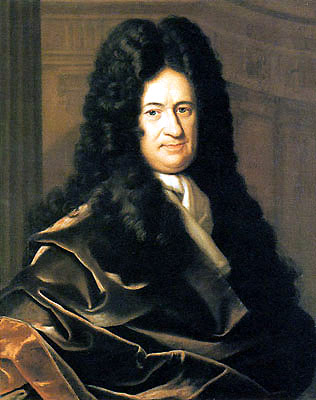
\includegraphics[width=0.384\textwidth]{leibniz.jpg}} 
		\subfigure[Isaac Newton]{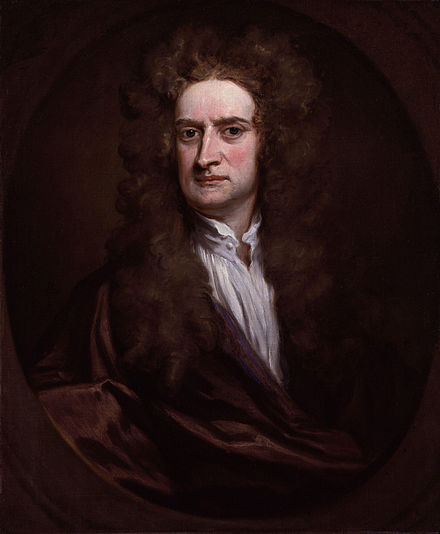
\includegraphics[width=0.4\textwidth]{newton.jpg}} 
		\caption{Die Entwickler der Differentialrechnung} 
	\end{figure} 
\end{frame}	

\begin{frame}{Differenzialrechnung - Newton}
	\begin{example}
		Beim freien, reibungsfreien Fall eines Regentropfens gibt die Wegfunktion
		\[
			s(t) = \frac{g}{2} t^{2} 
		\]
		den momentanen Ort in Abhängigkeit von der Fallzeit $t$ an. Wie groß ist die Geschwindigkeit in jedem Zeitpunkt $t$?
		
		Die mittlere Geschwindigkeit zwischen zwei Zeitpunkten $t_{1}$ und $t_{2}$ lässt sich einfach ausrechnen:
		\[
			\bar{v}_{t_{2}, t_{1}} = \frac{s(t_{2})-s(t_{1})}{t_{2}-t_{1}} = \frac{s(t_{1} + \Delta t) -s(t_{1})}{\Delta t}	
		\]
		mit $\Delta t := t_{2} - t_{1}$
	\end{example}
\end{frame}

\begin{frame}{Differenzialrechnung - Newton}
	\begin{example}
		Möchte man die Momentangeschwindigkeit bestimmen, muss man die Differenz $\Delta t := t_{2} - t_{1}$ beliebig klein machen. Da dann aber auch $\Delta s:=s(t_{1}+\Delta t) -  s(t_{1}) \to 0$ geht (weil der Weg ja stetig von der Zeit abhängt, der Tropfen macht im Flug ja keine Sprünge), muss man
		\[
			v(t):=\frac{ds(t)}{dt}:=\lim_{\Delta t \to 0} \frac{\Delta s(t)}{\Delta t}=\lim_{\Delta t \to 0} \frac{s(t+\Delta t)-s(t)}{\Delta t}
		\] 
		betrachten.
		Für das Weg-Zeit-Gesetz des Tropfens ist dann:
		\begin{align*}
			v(t)& =\lim_{\Delta t \to 0} \frac{\frac{g}{2}(t+\Delta t)^{2} - \frac{g}{2}t^{2}}{\Delta t} = \frac{g}{2} \lim_{\Delta t \to 0} \frac{t^{2} + 2t \Delta t + (\Delta t)^{2} -t^{2}}{\Delta t} \\
			& = \frac{g}{2} \lim_{\Delta t \to 0} \left( 2t + \Delta t \right) = \frac{g}{2} 2t = gt
		\end{align*}
	\end{example}
\end{frame}

\begin{frame}{Differenzialrechnung - Newton}
	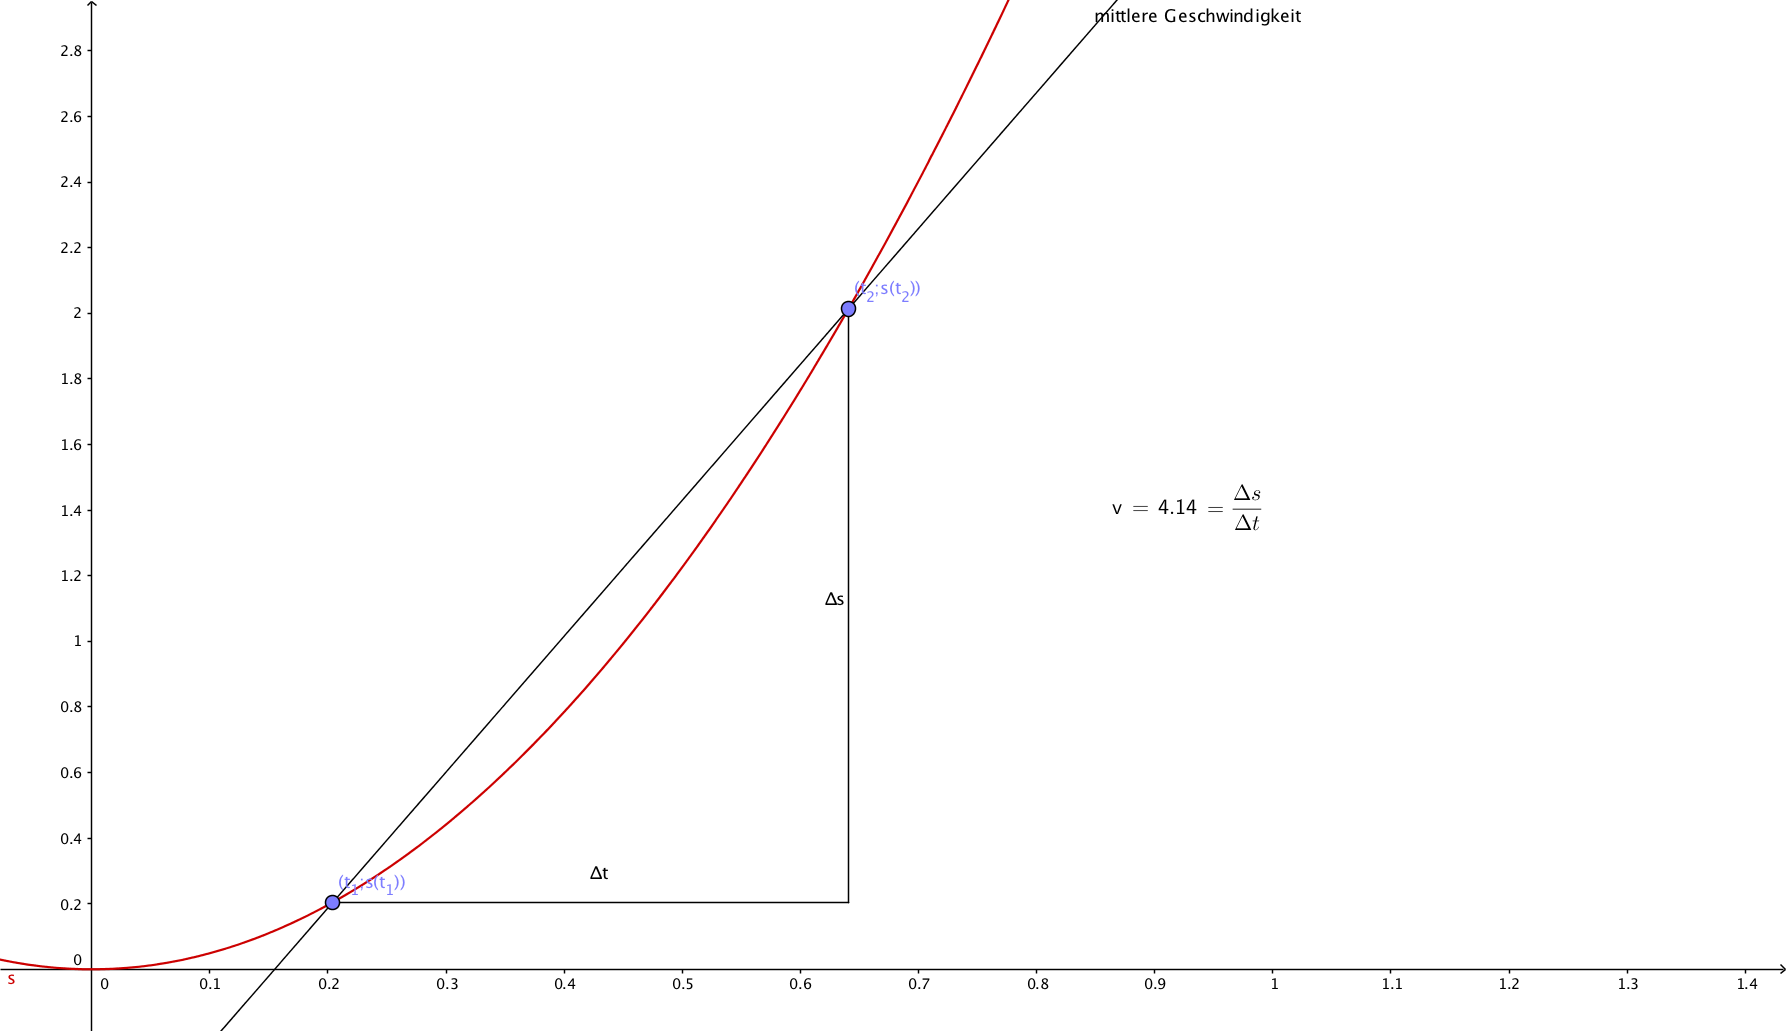
\includegraphics[width=14cm]{Geogebra/newton_geometrisch.png}
\end{frame}

\begin{frame}{Definition - Differenzialquotient}
	\begin{definition}{\small 	
		Existiert für eine (mindestens stetige) Funktion $y=f(x)$ an der Stelle $x_{0}$ der Grenzwert
		\[
			\lim_{\Delta x \to 0} \frac{\Delta y(x_{0})}{\Delta x} = \lim_{\Delta x \to 0} \frac{f(x_{0}+\Delta x)-f(x_{0})}{\Delta x} = \frac{dy(x_{0})}{dx} =: f' (x_{0}) =: y' (x_{0}) 
		\]
		so heißt dieser Grenzwert die \textbf{Ableitung von $f$} oder der \textbf{Differenzialquotient von $f$ an der Stelle $x_{0}$}.}
	
		Die Funktion heißt dann \textbf{differenzierbar an der Stelle $x_{0}$}.
		
		Wenn die Ableitung an allen Stellen $x \in D(f)$ existiert, kann man die Ableitung als eine Funktion $f'$ betrachten
		\[
			f'(x) := \lim_{\Delta x \to 0 } \frac{f(x+\Delta x)-f(x)}{\Delta x}  
		\] 
		und nennt diese Funktion $f'$ die \textbf{Ableitung von $f$}.
	\end{definition}
\end{frame}

\begin{frame}{Geometrische Deutung der Ableitung}
	\begin{bemerkung}
		Die erste Ableitung $f'(x_{0})$ gibt die Steigung der Tangente an den Graphen der Funktion $f$ an der Stelle $x_{0}$ an. Damit können also Aussagen gemacht werden über
		\begin{itemize}
			\item das Monotonieverhalten der Funktion $f$ und damit auch über
			\item evtl. Maxima und Minima der Funktion $f$.
		\end{itemize}
		Denn für den Differentialquotienten gilt ja:
		\[
			f'(x_{0}) = \lim_{x \to x_{0}} \frac{f(x)-f(x_{0})}{x-x_{0}} 
		\]
		und die rechte Seite ist 
		\begin{itemize}
			\item strikt positiv, wenn $f$ streng monoton wachsend
			\item positiv, wenn $f$ monoton wachsend
			\item strikt negativ, wenn $f$ streng monoton fallend bzw. 
			\item negativ, wenn $f$ monoton fallend ist.
	\end{itemize}
	\end{bemerkung}
\end{frame}

\begin{frame}{Beispiele für Ableitungen}
	\begin{example}
		Die \textbf{konstante Funktion} $f(x)=a$ ist überall differenzierbar und die Ableitung ist $f'(x) = 0$ für alle $x \in \mathbb{R}$. Denn
		\[
				\lim_{\Delta x \to 0} \frac{f(x+\Delta x) - f(x)}{\Delta x} = \lim_{\Delta x \to 0} \frac{a-a}{\Delta x} = \lim_{\Delta x \to 0} \frac{0}{\Delta x} = 0				
		\]
	\end{example}
	\begin{example}
		Die \textbf{lineare Funktion} $f(x)=mx+b$ mit $m,b \in \mathbb{R}$ ist überall differenzierbar und die Ableitung ist $f'(x) = m$ für alle $x \in \mathbb{R}$. Denn
		\begin{align*}
		\lim_{\Delta x \to 0} \frac{f(x+\Delta x) - f(x)}{\Delta x} & = \lim_{\Delta x \to 0} \frac{m(x+\Delta x)+b - (mx+b)}{\Delta x} \\ &= \lim_{\Delta x \to 0} \frac{m\Delta x}{\Delta x} = m				
		\end{align*}
	\end{example}
\end{frame}

\begin{frame}{Beispiele für Ableitungen}
	\begin{example}
		Die \textbf{quadratische Funktion} $f(x)=ax^{2}+bx+c$ mit $a,b,c \in \mathbb{R}$ ist überall differenzierbar und die Ableitung ist $f'(x) = 2ax+b$ für alle $x \in \mathbb{R}$. Denn
		\begin{align*}
		\lim_{\Delta x \to 0} & \frac{f(x+\Delta x) - f(x)}{\Delta x} \\ & = \lim_{\Delta x \to 0} \frac{a(x+\Delta x)^{2}+b(x+\Delta x) +c - (ax^{2}+bx+c)}{\Delta x} \\ &= \lim_{\Delta x \to 0} \frac{ax^{2} +2ax\Delta x +a(\Delta x)^{2} + bx +b \Delta x +c -ax^{2} - bx -c}{\Delta x} \\ &= \lim_{\Delta x \to 0  } \frac{2ax\Delta x + a(\Delta x)^{2} +b\Delta x}{\Delta x} = 2ax+b + \lim_{\Delta x \to 0} \frac{(a\Delta x)^{2}}{\Delta x}				
		\end{align*}
	\end{example}
\end{frame}

\begin{frame}{Beispiele für Ableitungen}
	\begin{example}
		Die \textbf{hyperbolische Funktion} $f(x)=\frac{1}{x}$ ist für alle $x\in D(f)=\mathbb{R}\setminus \{ 0 \}$ differenzierbar und die Ableitung ist $f'(x) = -\frac{1}{x^{2}}$ für alle $x \in D(f)$. Denn
		\begin{align*}
		\lim_{\Delta x \to 0} \frac{f(x+\Delta x) - f(x)}{\Delta x} & = \lim_{\Delta x \to 0} \frac{\frac{1}{x+\Delta x} - \frac{1}{x}}{\Delta x} \\ &= \lim_{\Delta x \to 0} \frac{\frac{x-(x+\Delta x)}{x(x+\Delta x)}}{\Delta x} \\ & = \lim_{\Delta x \to 0 } \frac{-\Delta x}{(\Delta x) x (x+\Delta x)} = -\frac{1}{x^{2}}			
		\end{align*}
	\end{example}	
\end{frame}

\begin{frame}{Ableitungen elementarer Funktionen}

{\LARGE $\begin{array}{cc}
	f(x)= x^{r} & f'(x)=r x^{r-1}  \\ 
	f(x)= \sqrt{x}& f'(x)=\frac{1}{2\sqrt{x}}  \\ 
	f(x)= \frac{1}{\sqrt{x}}& f'(x)= -\frac{1}{2\sqrt{x^{3}}}  \\ 
	f(x)= \log_{a} x & f'(x)=\frac{1}{x \ln a}  \\ 
	f(x)= a^{x}& f'(x)= a^{x} \ln a  \\ 
	f(x)= \sin x& f'(x)=\cos x \\ 
	f(x)= \cos x& f'(x)= -\sin x	  \\
\end{array} $
}
\end{frame}

\begin{frame}{Zweite und höhere Ableitungen}
	\begin{definition}
		Sofern man die Ableitung $f'$ einer Funktion $f$ wieder ableiten kann, so nennt man die Ableitung der Ableitungsfunktion $f'$ die zweite Ableitung der Funktion $f$ und bezeichnet sie mit $f''$.
		
		Eine Funktion $f$ heißt n-mal differenzierbar, wenn die n-te Ableitung existiert:
		\[
			\frac{d^{n}f(x)}{dx^{n}} = \frac{d}{dx}\frac{d^{n-1}f(x)}{dx^{n-1}} = f^{(n)}(x)
		\]
	\end{definition}
\end{frame}

\begin{frame}{Ableitungsregeln}
	\begin{theorem}
		Für zwei differenzierbare Funktion $f$ und $g$ gilt:
		\begin{itemize}
			\item Die Summe $f+g$ ist differenzierbar, also die Funktion $\left( f+g \right) (x) := f(x)+g(x)$ und $\left(f+g\right)'(x) = f'(x)+g'(x)$
			\item Die Differenz $f-g$ ist differenzierbar, also die Funktion $\left(f-g\right)(x) := f(x)-g(x)$ und $\left(f-g\right)'(x) = f'(x)-g'(x)$
			\item Die Funktion $c \cdot f$ mit einer Konstanten $c$ ist differenzierbar, also die Funktion $\left(c\cdot f\right)(x) := c\cdot f(x)$ und $\left(cf\right)'(x) = c\cdot f'(x)$				
			\item Die Funktion $f + c$ mit einer Konstanten $c$ ist differenzierbar, also die Funktion $f(x) + c$ und ihre Ableitung ist gleich $f'(x)$				
		\end{itemize}
	\end{theorem}
\end{frame}

\begin{frame}{Produktregel für die Ableitung}
	\begin{theorem}
		Das Produkt $h=f \cdot g$ zweier differenzierbarer Funktionen $f$ und $g$ ist differenzierbar und es gilt:
		\[
		h'(x)=\left( f\cdot g \right)' (x) = f'(x)\cdot g(x) + f(x)\cdot g'(x) 
		\]
	\end{theorem}
	\begin{proof}[Beweis]{
\tiny

 		\begin{align*}
		h'(x) & = \lim_{\Delta x \to 0} \frac{h(x+\Delta x) - h(x)}{\Delta x} \\
		& = \lim_{\Delta x \to 0} \frac{f(x+\Delta x)\cdot g(x+\Delta x) - f(x)\cdot g(x)}{\Delta x} \\
		& = \lim_{\Delta x \to 0} \frac{f(x+\Delta x)\cdot g(x+\Delta x) - f(x)\cdot g(x)}{\Delta x} \\
		& = \lim_{\Delta x \to 0} \frac{f(x+\Delta x)\cdot g(x+\Delta x) - f(x)\cdot g(x+\Delta x) + f(x)\cdot g(x+\Delta x)- f(x)\cdot g(x)}{\Delta x}  \\			
		& = \lim_{\Delta x \to 0} \frac{\left( f(x+\Delta x) - f(x)\right)\cdot g(x+\Delta x) + f(x)\cdot \left( g(x+\Delta x )- \cdot g(x)\right) }{\Delta x}  \\			
		& = f'(x)\cdot g(x) + f(x)\cdot g'(x)
		\end{align*}}
	\end{proof}
\end{frame}

\begin{frame}{Quotientenregel für die Ableitung}

{\small	\begin{theorem}
		Der Quotient $h=\frac{f}{g}$ zweier differenzierbarer Funktionen $f$ und $g$ ist differenzierbar an allen Stellen, an denen $g(x)\neq 0$ ist und es gilt:
		\[
		h'(x)=\left( \frac{f}{g} \right)' (x) = \frac{f'(x)\cdot g(x) - f(x)\cdot g'(x)}{g^{2}(x)} 
		\]
	\end{theorem}
}	\begin{proof}[Beweis]{\tiny
		\begin{align*}
		h'(x) & = \lim_{\Delta x \to 0 } \frac{1}{\Delta x} \left( \frac{f(x+\Delta x)}{g(x+\Delta x)} - \frac{f(x)}{g(x)} \right) \\
		&= \lim_{\Delta x \to 0 } \frac{1}{\Delta x} \left( \frac{f(x+\Delta x) g(x)}{g(x+\Delta x) g(x)} - \frac{f(x)g(x+\Delta x)}{g(x)g(x+\Delta x)} \right) \\
		&= \lim_{\Delta x \to 0 } \frac{1}{g(x+\Delta x) g(x)} \left( \frac{f(x+\Delta x) g(x)- f(x)g(x+\Delta x)}{\Delta x} \right) \\
		&= \lim_{\Delta x \to 0 } \frac{1}{g(x+\Delta x) g(x)} \left( \frac{f(x+\Delta x) g(x)-f(x)g(x)+f(x)g(x)- f(x)g(x+\Delta x)}{\Delta x} \right) \\
		&= \lim_{\Delta x \to 0 } \frac{1}{g(x+\Delta x) g(x)} \left(  \frac{\left(f(x+\Delta x) -f(x)\right) g(x)-f(x)\left( g(x+\Delta x) -g(x)\right) }{\Delta x} \right) 				
\end{align*}}
	\end{proof}
\end{frame}

\begin{frame}{Kettenregel - Motivation}
	\begin{bemerkung}
		Bisher wurden Ableitungen elementarer Funktionen sowie Summen, Produkte und Quotienten behandelt.
		
		Damit sind aber Ableitung von Funktionen wie z.B. 
		\[
			e^{(4x^{2}-3x+2)} \qquad \text{ oder }\qquad \sin (3x+\alpha)
		\]
		nicht möglich.
		
		Diese Funktionen sind \textbf{verkettete Funktionen} $h(x):=f(g(x))$, bei denen man zuerst die \textbf{innere Funktion} $g$ auf $x$ anwendet und dann das Ergebnis $g(x)$ in die \textbf{äußere Funktion} $f$ einsetzt.
		
		In den Beispielen oben ist $g(x)=4x^{2}-3x+2$ und $f(g)=e^{g}$ bzw. $g(x)=3x+\alpha$ und $f(g)=\sin (g)$.
	\end{bemerkung}
\end{frame}

\begin{frame}{Kettenregel für die Ableitung\footnote{Ableitung der mittelbaren Funktion}}
	\begin{theorem}
		Für zwei auf ihrem jeweiligen Definitionsbereich differenzierbare Funktionen $f$ und $g$ mit $W(g) \subset D(f)$ (d.h. man kann die $y$-Werte von $g$ in $f$ einsetzen.) sei $h$ die Verkettung der beiden Funktionen, also
		\[
			h(x):= f(g(x)) \qquad \forall x \in D(f)
		\]
		Dann gilt für die Ableitung von $h$:
		\[
			h'(x)=f'(g(x)) \cdot g'(x) \qquad \forall x \in D(f)
		\]
		Man nennt $f'(g(x))$ die \textbf{äußere Ableitung} und $g'(x)$ \textbf{die innere Ableitung}.
	\end{theorem}
\end{frame}

\begin{frame}{Kettenregel - sowas wie ein Beweis}

{\small 	\begin{bemerkung}
				Betrachtet man die äußere Funktion als Funktion von $g$, so ist
				\[
				\frac{df}{dg} = \lim_{\Delta g \to 0} \frac{f(g+\Delta g)-f(g)}{\Delta g} = \lim_{\Delta g \to 0} \frac{\Delta f}{\Delta g}
				\]	
				und entsprechend ist für die innere Funktion $g$ als Funktion von $x$
				\[
				\frac{dg}{dx} = \lim_{\Delta x \to 0} \frac{g(x+\Delta x)-g(x)}{\Delta x} = \lim_{\Delta x \to 0} \frac{\Delta g}{\Delta x}
				\]	
		Für die verkettete Funktion $h(x)=f(g(x))$ wäre der Differenzialquotient
		\begin{align*}
			\frac{dh}{dx} & = \lim_{\Delta x \to 0} \frac{h(x+\Delta x)-h(x)}{\Delta x} = \lim_{\Delta x \to 0} \frac{\Delta h}{\Delta x} \\
			& = \lim_{\Delta x \to 0} \frac{\Delta (f(g(x)))}{\Delta x} = \lim_{\Delta x \to 0 } \left( \frac{\Delta f(g(x))}{\Delta g(x)} \frac{\Delta g(x)}{\Delta x} \right)  \\
			& = \lim_{\Delta g \to 0 } \frac{\Delta f(g)}{\Delta g} \lim_{\Delta x \to 0 } \frac{\Delta g(x)}{\Delta x} = f'(g(x))\cdot g'(x)
		\end{align*}		
		\end{bemerkung}
}\end{frame}

\begin{frame}{Ableitung der Umkehrfunktion}
	\begin{theorem}
		Für die Umkehrfunktion $f^{-1}$ einer differenzierbaren Funktion $f$ gilt:
		\[
			\left(f^{-1}\right)' (x) = \frac{1}{f'(f^{-1}(x))}
		\]
	\end{theorem}
{\small	\begin{bemerkung}
		Man kann sich das so merken:
		\begin{align*}
		& f\left(f^{-1}(x)\right) & = x \\ & \Rightarrow \frac{d}{dx} f\left(f^{-1}(x)\right) & = \frac{d}{dx} x = 1 \\  & \Rightarrow f'\left( f^{-1}(x) \right)  \left( f^{-1} \right)'(x) & = 1 \\ 
		& \Rightarrow \left( f^{-1} \right)'(x) & = \frac{1}{f'(f^{-1}(x))}
		\end{align*}
	\end{bemerkung}}
\end{frame}

\begin{frame}{Regel von l'Hospital\footnote{Guillaume François Antoine, Marquis de L’Hospital hat die Regel nicht selbst entdeckt, sondern von Johann Bernoulli gekauft!}}

{\footnotesize	\begin{bemerkung}
		Die Regel von l'Hospital dient zur Berechnung von Grenzwerten $\lim_{x \to x_{0}}\frac{f(x)}{g(x)}$, bei denen unbestimmte Ausdrücke der Form
		\[
		\frac{\infty}{\infty} \quad \frac{0}{0} \quad 0\cdot \infty \quad 0^{0} \quad 1^{\infty} \quad \infty - \infty
		\]
	\end{bemerkung}
	\begin{theorem}
		Sind $f$ und $g$ in einem Intervall um $x_{0}$ differenzierbare Funktionen und $g(x)\neq 0$ in einer Umgebung von $x_{0}$, aber entweder 
		\begin{itemize}
			\item 
		$\lim_{x \to x_{0}} g(x) = 0$ und $\lim_{x \to x_{0}} f(x) = 0$ oder
		\item $\lim_{x \to x_{0}} g(x) = \infty$ und $\lim_{x \to x_{0}} f(x) = \infty$
	\end{itemize} 
	wobei der Grenzwert
	\[
		\lim_{x \to x_{0}} \frac{f'(x)}{g'(x)}
	\]
	existiert, so gilt:
	\[
		\lim_{x \to x_{0}} \frac{f(x)}{g(x)} = \lim_{x \to x_{0}} \frac{f'(x)}{g'(x)}
	\]
	\end{theorem}}
\end{frame}

\begin{frame}{Regel von l'Hospital - sowas wie ein Beweis}
	\begin{bemerkung}
		Für den Fall $f(x_{0})=g(x_{0}) = 0$ kann man das anschaulich so erklären:
		\[
			\lim_{x \to x_{0}} \frac{f(x)}{g(x)} = \lim_{x \to x_{0}} \frac{f(x)-f(x_{0})}{g(x)-g(x_{0})} = \lim_{x \to x_{0}} \frac{\frac{f(x)-f(x_{0})}{x-x_{0}}}{\frac{g(x)-g(x_{0})}{x-x_{0}}} = \frac{f'(x_{0})}{g'(x_{0})}
		\]
		Im ersten Schritt hat man hier im Zähler und im Nenner jeweils eine 0 hinzugefügt, im zweiten Schritt mit $x-x_{0}$ erweitert und dann die Definition der Ableitung benutzt.
		
		Die verbleibenden Grenzwertfälle müssen durch Äquivalenzumformungen auf diese beiden Fälle zurückgeführt werden.
	\end{bemerkung}
\end{frame}

\begin{frame}{Geometrische Deutung der 1. Ableitung}
	\begin{bemerkung}
		Die erste Ableitung $f'$ einer Funktion $f$ gibt die Steigung der Tangente an den Graphen der Funktion f an. Daher können mit Hilfe der 1. Ableitung Aussagen über das Monotonie-Verhalten der Funktion $f$ gemacht werden:
		\begin{itemize}
			\item Falls $f'(x_{0})>0$, so ist die Funktion in einer Umgebung von $x_{0}$ streng monoton wachsend.
			\item Falls $f'(x_{0})<0$, so ist die Funktion in einer Umgebung von $x_{0}$ streng monoton fallend.	
		\end{itemize}  
	\end{bemerkung}
\end{frame}

\begin{frame}{Relative/lokale Extrema - Definition}
	\begin{definition}
		Die Funktion $f$ hat an der Stelle $x_{0}$ ein \textbf{relatives/lokales Maximum}, wenn für alle $x$ in einer Umgebung von $x_{0}$ gilt: 
		\[
		f(x_{0})>f(x)
		\]
		
		Die Funktion $f$ hat an der Stelle $x_{0}$ ein \textbf{relatives/lokales Minimum}, wenn für alle $x$ in einer Umgebung von $x_{0}$ gilt: 
		\[
		f(x_{0})<f(x)
		\]
		
		In beiden Fällen spricht man von einem \textbf{relativen/lokalen Extremum}.
	\end{definition}
\end{frame}
\begin{frame}{Lokale Extrema - Notwendige Bedingung}
	\begin{theorem}[Fermat]
		Falls eine differenzierbare Funktion $f$ im Punkt $x_{0}$ ein relatives Extremum hat, so gilt dort:
		\[
			f'(x_{0}) = 0
		\]
		Die Bedingung ist \textbf{notwendig}, aber \textbf{nicht hinreichend}, denn es gibt Funktionen mit waagerechter Tangente, die dort kein Extremum haben.
	\end{theorem}
\end{frame}

\begin{frame}{Zwischenwertsatz - Satz von Rolle - Mittelwertsatz}

{\footnotesize	\begin{theorem}[Zwischenwertsatz]
		Für eine stetige Funktion $f$ mit $f(a) \leq f(b)$ und $a<b$ gilt:
		\[
		\text{Für alle }y_{0} \text{ mit } f(a)\leq y_{0} \leq f(b) \text{ gibt es ein } x_{0} \text{ mit } a \leq x_{0} \leq b \text{ und } f(x_{0})=y_{0}
		\]
	\end{theorem}
	\begin{theorem}[Rolle]
		Für jede differenzierbare Funktion $f$ mit $f(a)=f(b)$ gibt es eine Stelle $x_{0}$ mit $f'(x_{0}) = 0$.
	\end{theorem}
	\begin{theorem}[Mittelwertsatz]
		Ist eine Funktion $f$ im Intervall $[a, b]$ stetig und in $]a, b[$ differenzierbar, dann gibt es eine Stelle $x_{0}$ mit $a < x_{0} < b$ und 
		\[
			f'(x_{0}) = \frac{f(b)-f(a)}{b-a}
		\]
	\end{theorem}
}
\end{frame}

\begin{frame}{Extrema - notwendige und hinreichende Bedingung}
	\begin{theorem}
		Eine differenzierbare Funktion $f$ besitzt an der Stelle $x_{0}$ ein relatives/lokales Extremum, wenn gilt:
		\[
			f'(x_{0}) = 0 \qquad \text{und}\qquad f^{(n)}(x_{0}) \neq 0 \text{ für ein gerades } n. \footnote{z.B. und meistens $n=2$} 
		\]
		Genauer ist:
		\begin{itemize}
			\item an der Stelle $x_{0}$ ein \textbf{relatives Maximum}, falls $f'(x_{0})=0$ und $f^{(n)}(x_{0})<0$ für ein gerades $n$.
			\item an der Stelle $x_{0}$ ein \textbf{relatives Minimum}, falls $f'(x_{0})=0$ und $f^{(n)}(x_{0})>0$ für ein gerades $n$.
		\end{itemize}
	\end{theorem}
\end{frame}

\begin{frame}{Randextrema}
\begin{bemerkung}
	Bei Funktionen, deren Definitionsbereich eingeschränkt (z.B. auf ein Intervall) ist, kann es sein, dass Extrema an den Rändern des Definitionsbereiches angenommen werden, obwohl dort die (dann meist nur einseitig definierte Ableitung) nicht null ist.
	
	Beispiel: $f(x)=\sqrt{1-x^{2}}$
	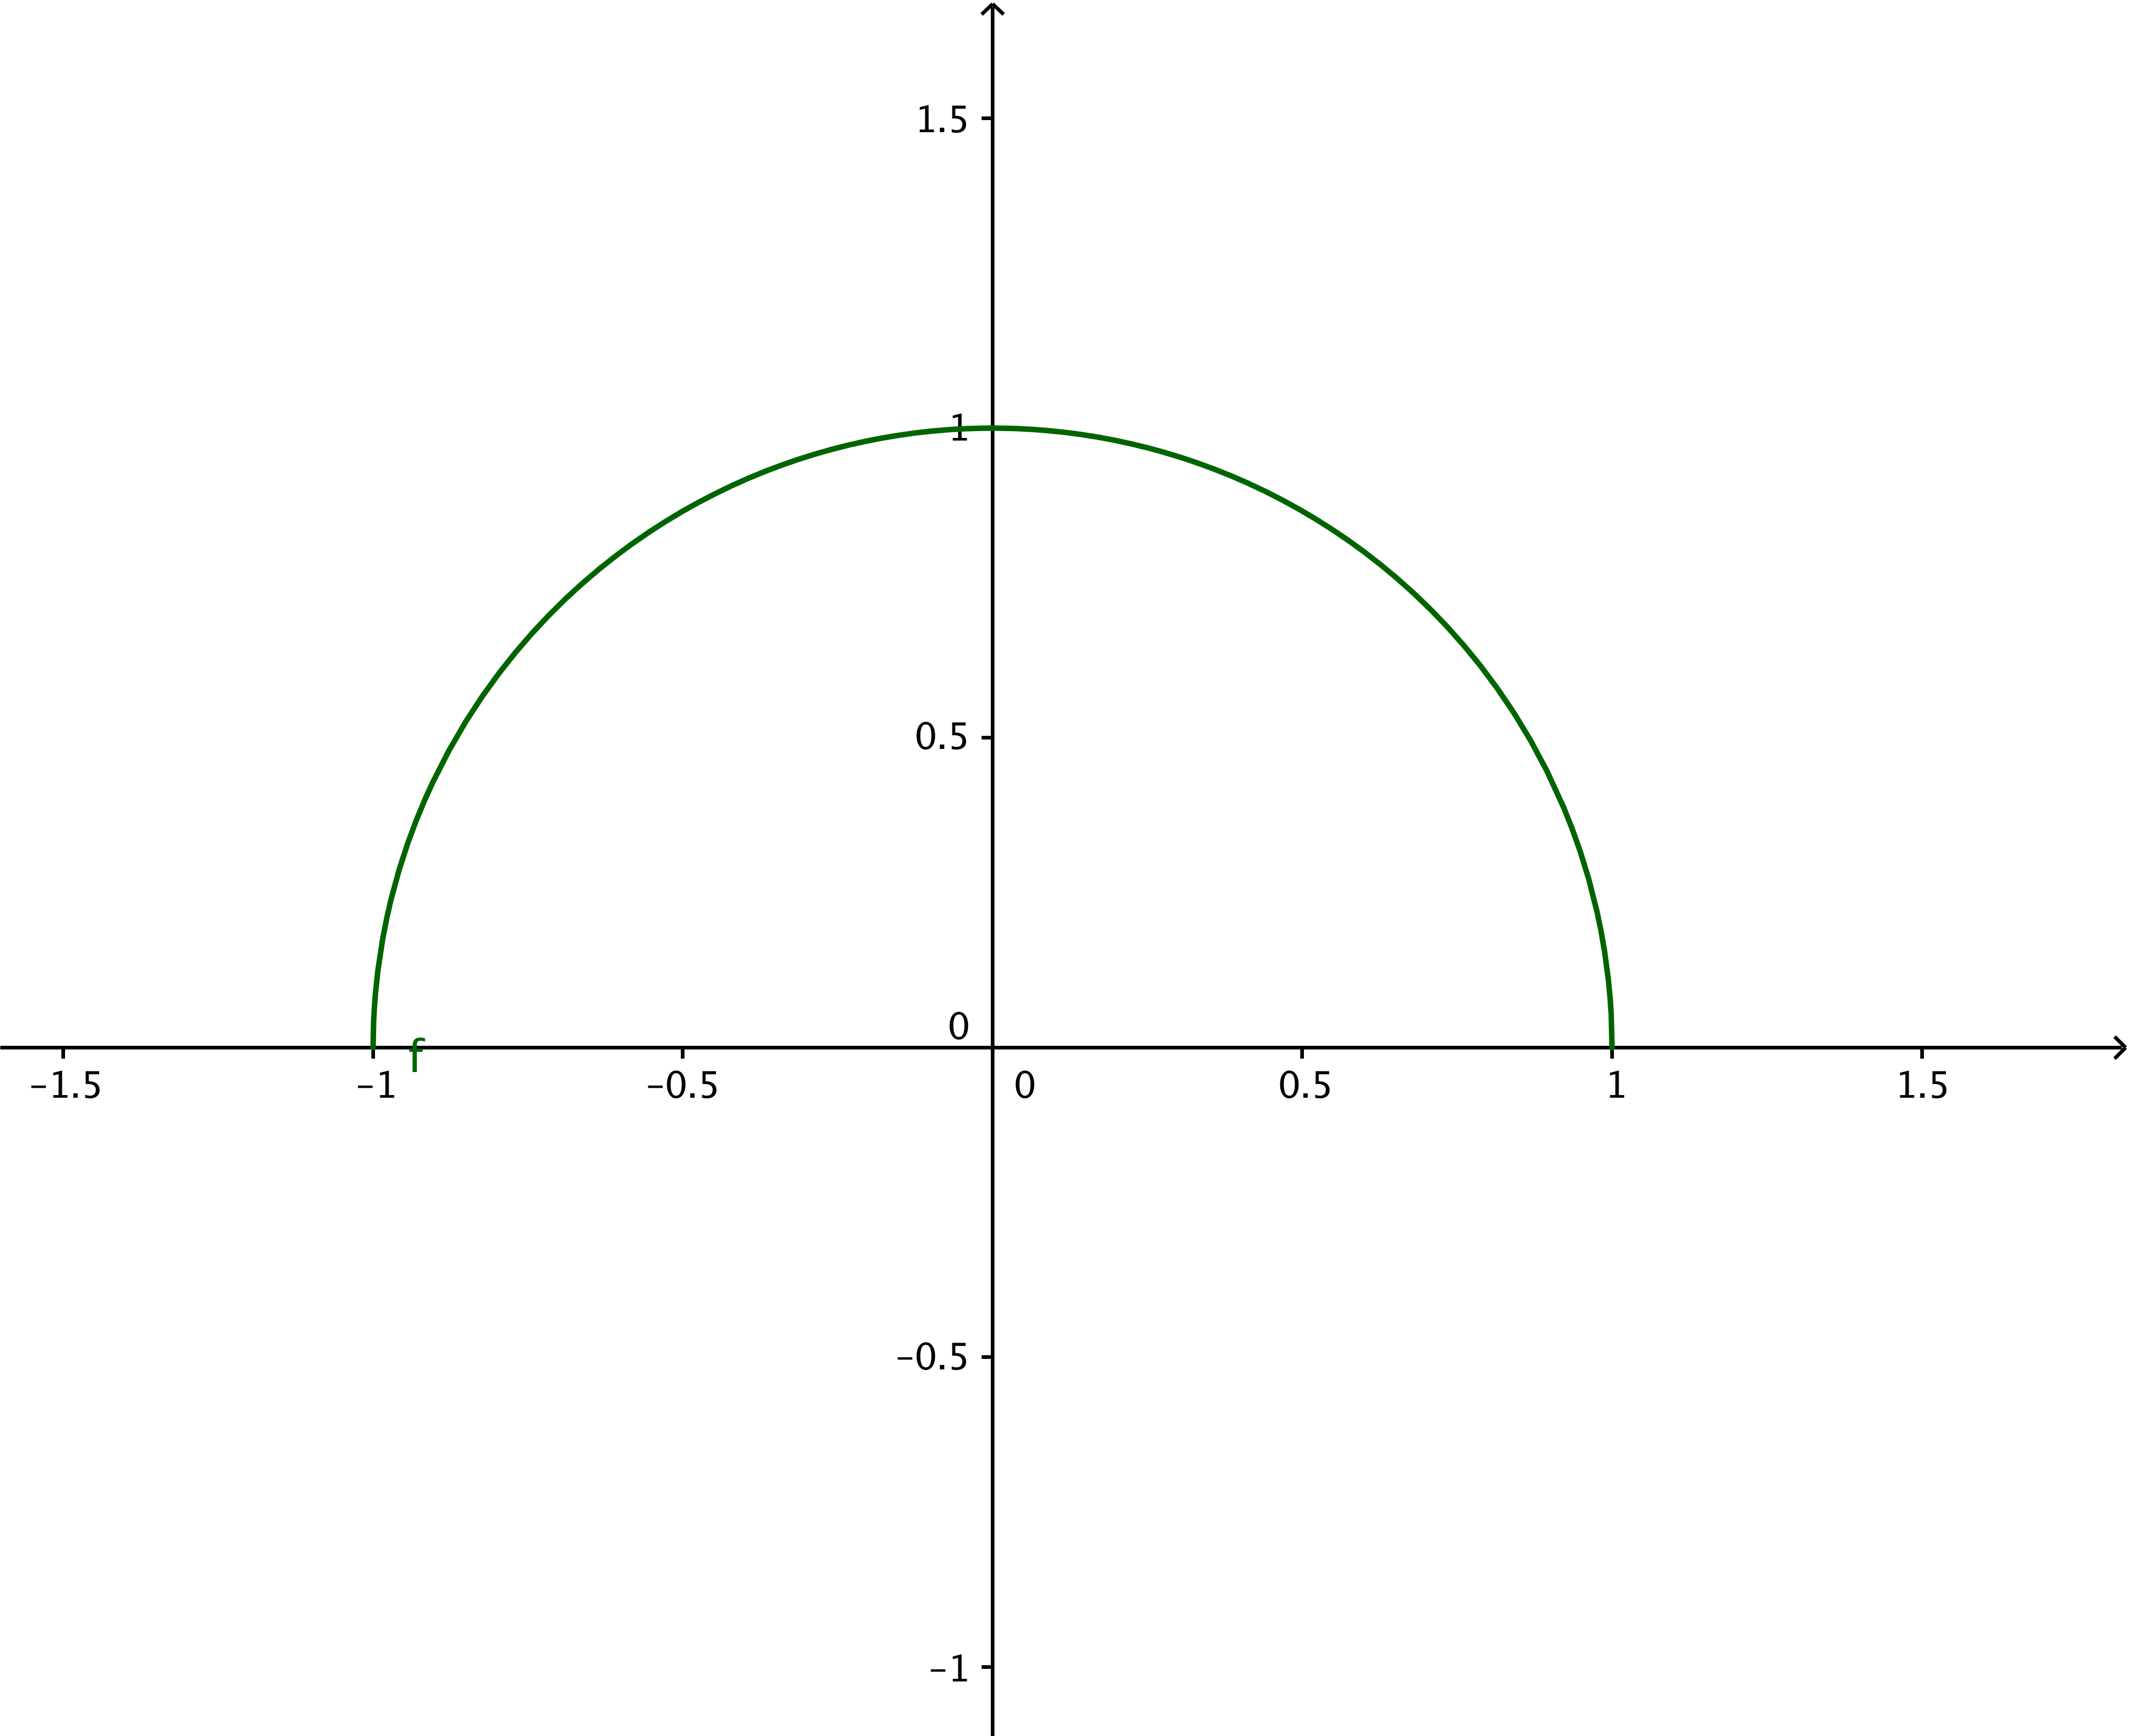
\includegraphics[width=9cm]{halbkreis}
\end{bemerkung}	
\end{frame}

\begin{frame}{Geometrische Deutung der 2. Ableitung}
\begin{bemerkung}
	Die erste Ableitung einer Funktion $f$ gibt deren Steigung an jeder Stelle an. Die Veränderung dieser Steigung gibt die zweite Ableitung (als Ableitung der 1. Ableitung) an.
	
	Wenn die Steigung einer Funktion zunimmt, also die 2. Ableitung positiv ist, ist die Funktion linksgekrümmt.
	
	Wenn die Steigung einer Funktion abnimmt, also die 2. Ableitung negativ ist, ist die Funktion rechtsgekrümmt.
\end{bemerkung}
\begin{definition}
	Für eine zweimal differenzierbare Funktion $f$ gilt:
	\begin{itemize}
		\item $f$ heißt streng \textbf{linksgekrümmt} oder \textbf{streng konvex} im Punkt $x_{0}$, wenn $f''(x_{0})>0$ ist.
		\item $f$ heißt streng \textbf{rechtsgekrümmt} oder \textbf{streng konkav} im Punkt $x_{0}$, wenn $f''(x_{0})<0$ ist.
	\end{itemize} 
\end{definition}
\end{frame}

\begin{frame}{Wende- und Sattelpunkte}
\begin{definition}
	Die Stellen, an denen eine Funktion ihr Krümmungsverhalten von rechts- auf linksgekrümmt (oder umgekehrt) ändert, heißen \textbf{Wendepunkte}.
	
	Wenn zudem die Tangente an einem Wendepunkt waagerecht ist, nennt man den Wendepunkt einen \textbf{Sattelpunkt}. 	
\end{definition}
\begin{theorem}
	Eine dreimal differenzierbare Funktion $f$ besitzt an der Stelle $x_{0}$ einen Wendepunkt genau dann, wenn 
	\[
		f''(x_{0}) = 0 \quad \text{und} \quad f'''(x_{0})\neq 0
	\]
	ist.
	Wenn zudem $f'(x_{0}) = 0$ ist, so hat die Funktion an der Stelle $x_{0}$ einen Sattelpunkt.
\end{theorem}
\end{frame}
\begin{frame}{Krümmungseigenschaften}
\begin{bemerkung}
	Die dritte Ableitung $f'''$ einer Funktion $f$ gibt dabei offenbar an, in welche Richtung der Krümmungswechsel stattfindet\footnote{natürlich nur, wenn $f''(x_{0})=0$ ist}:
	\begin{itemize}
		\item Falls $f'''(x_{0})>0$ ist, so wechselt die Krümmung von Rechts- auf Linkskrümmung.
		\item Falls $f'''(x_{0})<0$ ist, so wechselt die Krümmung von Links- auf Rechtskrümmung.
	\end{itemize}
\end{bemerkung}
\end{frame}

\begin{frame}{Kurvendiskussion}
	\begin{bemerkung}
		Alle bisherigen Hilfmittel zur Untersuchung einer Funktion lassen sich zusammenfassen in einer \textbf{Kurvendiskussion}. Diese beinhaltet:
		\begin{enumerate}
			\item Bestimmung der Definitionsmenge und der Wertemenge
			\item Untersuchung auf Symmetrie und Periodizität
			\item Bestimmung von Nullstellen, Verhalten an Definitionslücken, Polstellen, Verhalten für $x \to \pm \infty$
			\item Untersuchung auf Stetigkeit und Differenzierbarkeit
			\item Bestimmung der Extrema und Wendepunkte
			\item Graph der Funktion
		\end{enumerate}
	\end{bemerkung}
\end{frame}

\begin{frame}{Extremwertaufgaben}
	\begin{example}
		Aus einem rechteckigen Blech mit den Seitenlängen $a$ und $b$ ist nach dem Herausschneiden von quadratischen Flächen der Kantenlänge $x$ an den Ecken ein oben offener Kasten mit möglichst großem Volumen zu formen.
		
		Für das Volumen gilt:
		\[
		V(x)=\left( a-2x \right) \left( b-2x \right) x = 4x^{3} -2(a+b)x^{2} +abx 
		\]
		
		Dessen Maximum könnte an den Stellen sein, wo die Ableitung verschwindet:
		
		\[
		V'(x)=12x^{2} -4 (a+b)x + ab \overset{!}{=} 0 \]
		also an den Stellen
		\[
		x_{1,2} = \frac{1}{6} \left( a+b\pm \sqrt{a^2+b^2-ab} \right)
		\]
	\end{example}
\end{frame}

\begin{frame}{Extremwertaufgaben}
	\begin{example}
		Zur Überprüfung, ob es sich wirklich an beiden Stellen um Maxima handelt, setzt man diese Stellen in die zweite Ableitung
		\[
			V''(x)=24x-4(a+b)
		\]
		ein:
		\[
		V''(x_{1})= 24 x_{1} -4(a+b) = 4\sqrt{a^2+b^2-ab} > 0
		\]
		und 
		\[
		V''(x_{2})= 24 x_{2} -4(a+b) = - 4\sqrt{a^2+b^2-ab} < 0		
		\]
		Also ist nur an der Stelle $x_{2}$ die Volumenfunktion $V(x)$ rechtsgekrümmt mit waagerechter Tangente und entsprechend handelt es sich bei dieser Stelle $x_{2}$ und das lokale Maximum. Das maximale Volumen ist dann $V(x_{2})$.
	\end{example}
\end{frame} 
\section{Integral- und Flächenberechnung}
\subsection{Einführung - Treppensummen}
\subsubsection{Flächenberechnung}
\begin{frame}{Integral konstanter Funktionen}
	Arbeit ist physikalisch definiert als Kraft mal Weg, also für eine konstante Kraft $F(x)=F$
	\[
		W=F \cdot (x_{2} - x_{1}) 
	\]
	wenn $x_{1}$ und $x_{2}$ der Start- und der Endpunkt des Weges sind, über den die Kraft $F$ ausgeübt wird. Das entspricht aber der Fläche zwischen dem Funktionsgraphen und der $x$-Achse zwischen den Stellen $x_{1}$ und $x_{2}$
	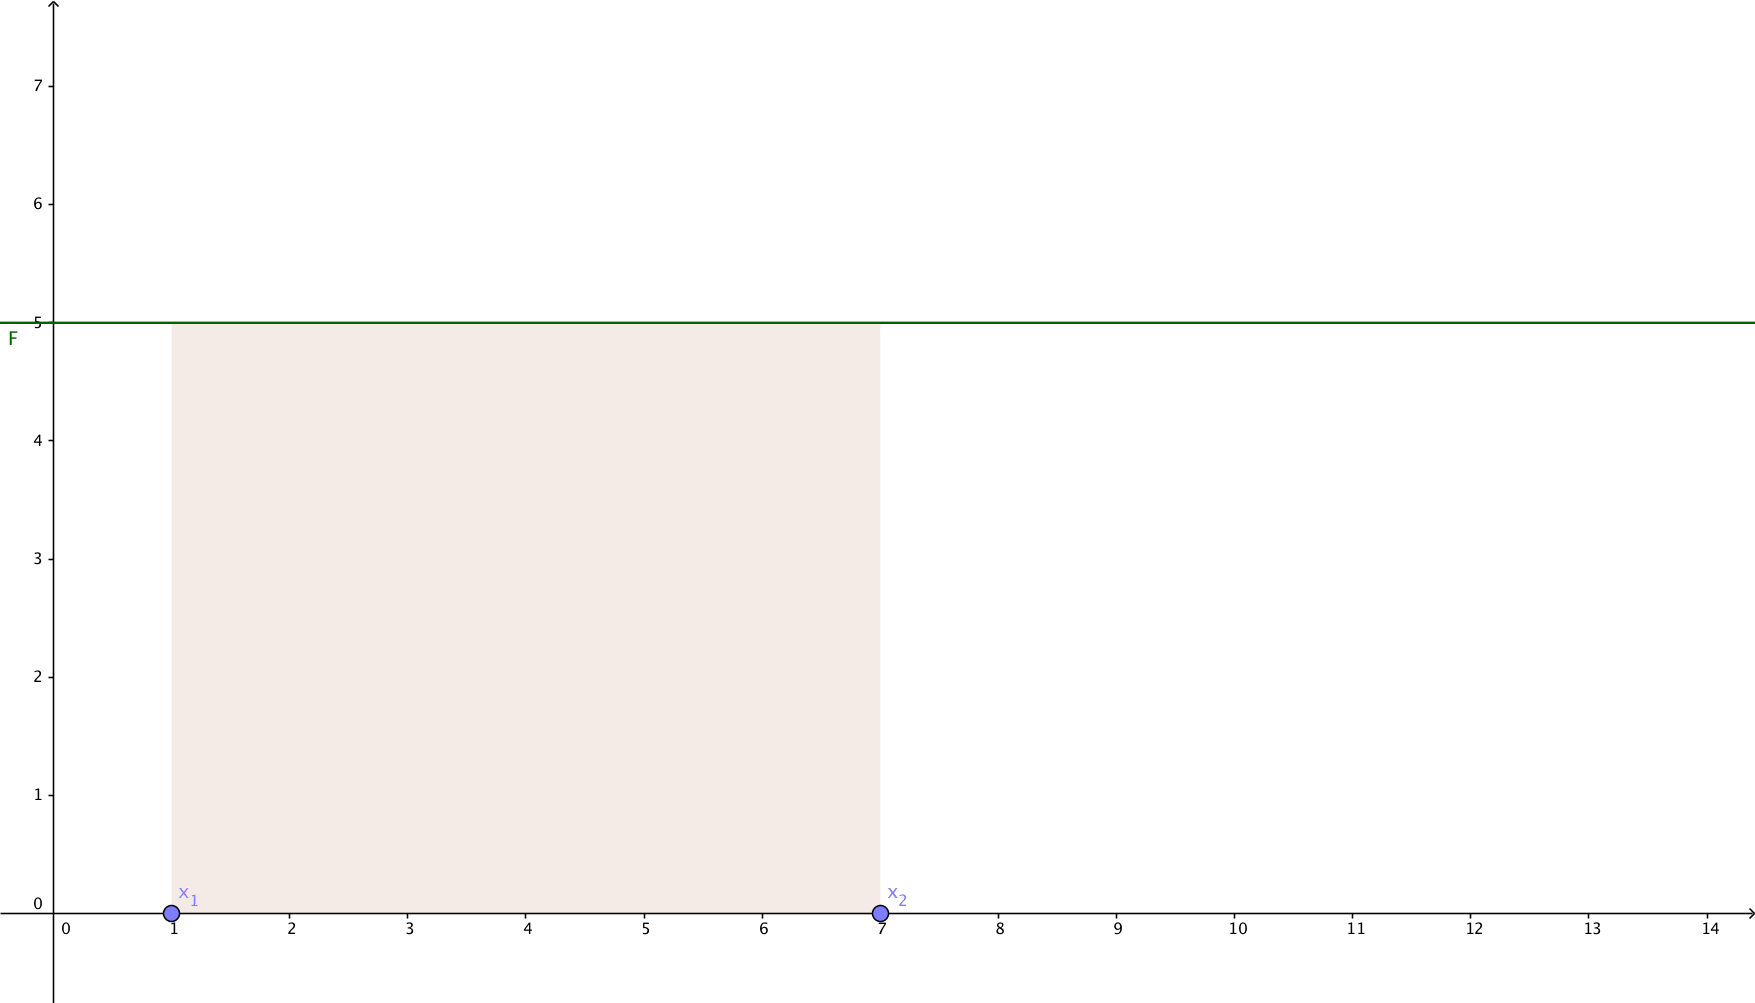
\includegraphics[width=8cm]{integral_konstantefunktion}
\end{frame}

\begin{frame}{Integral linearer Funktionen}
	Für eine nicht-konstante, aber lineare vom Weg abhängige Kraft $F(x)=a \cdot x + b$ ist die Berechnung der Arbeit schon etwas schwieriger, weil nun die Kraft vom (momentanen) Ort abhängt:
	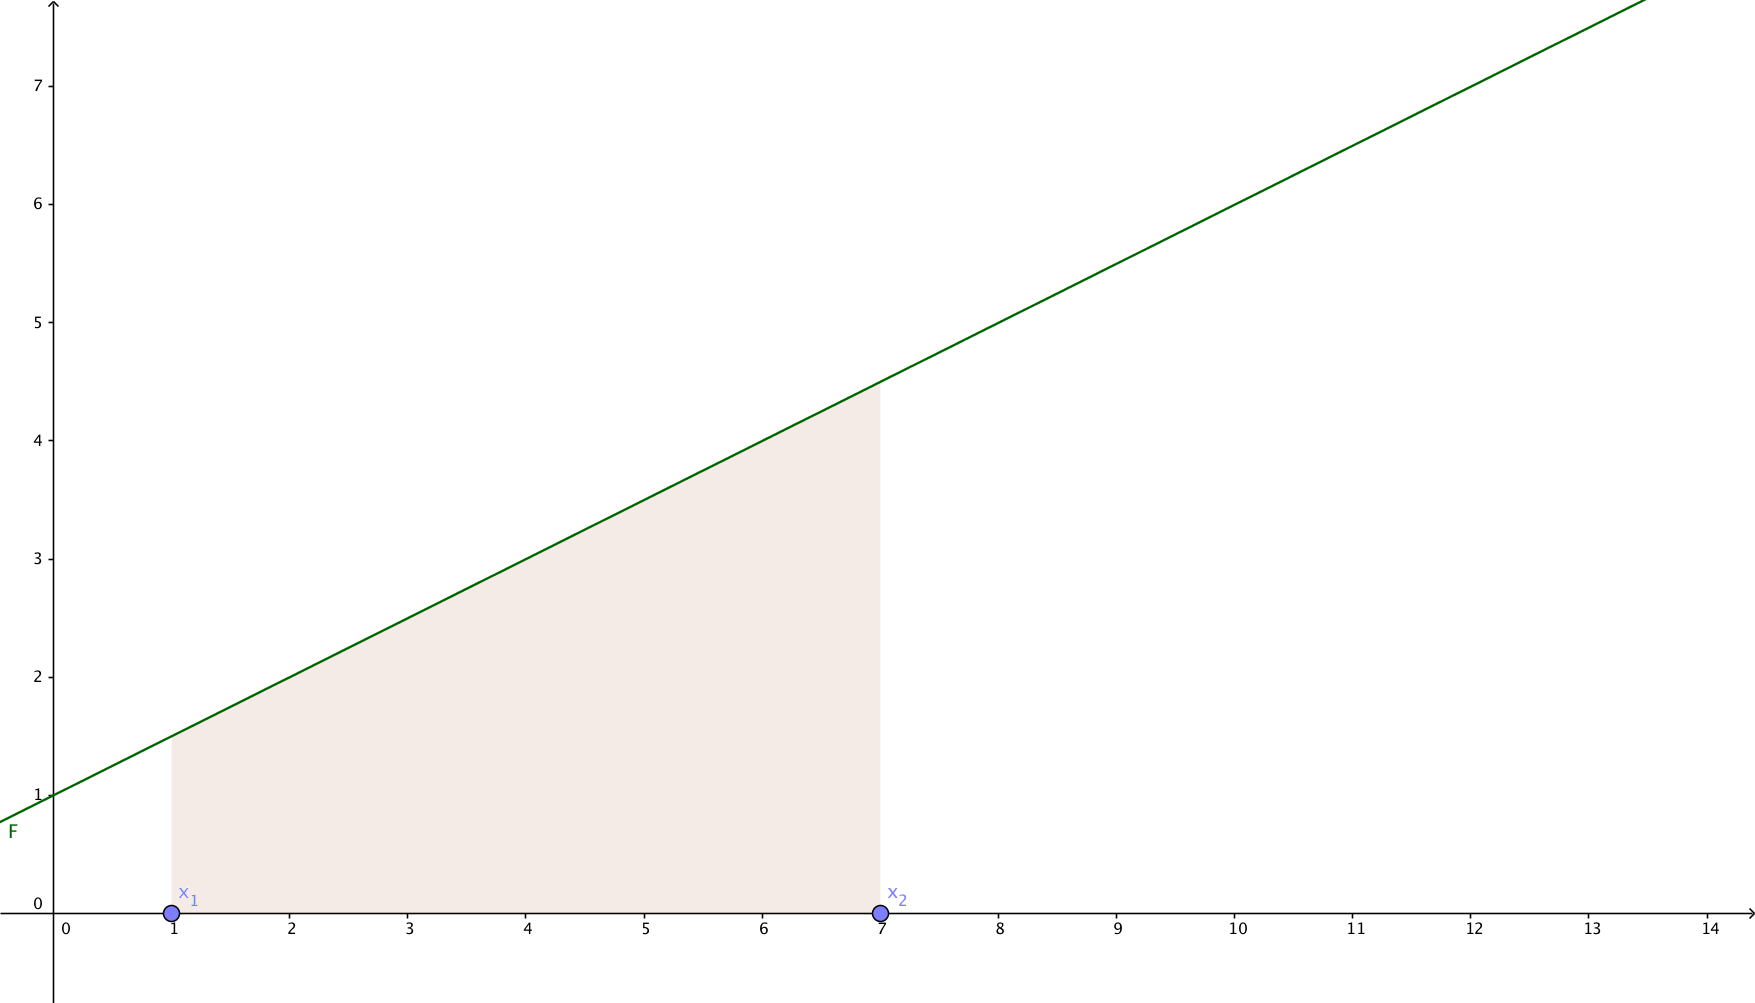
\includegraphics[width=8cm]{integral_linearefunktion}
	
	Geometrisch (Trapezformel) findet man hier:
\scriptsize{	\[
		W = \frac{1}{2} (F(x_{2})+F(x_{1})) (x_{2}-x_{1}) = \frac{1}{2} (ax_{2} + b + (ax_{1} + b)) (x_{2}-x_{1}) = ax_{2}^2-ax_{1}^{2} + b(x_{2}-x_{1})
	\]}
\end{frame}

\begin{frame}{Integral quadratische Funktion}
	\tiny{
	Für die quadratische Funktion $F(x)=x^{2}$ wir das ganze komplizierter, daher verwenden wir hier $N$ einfache (untere) Treppenfunktionen:
	
	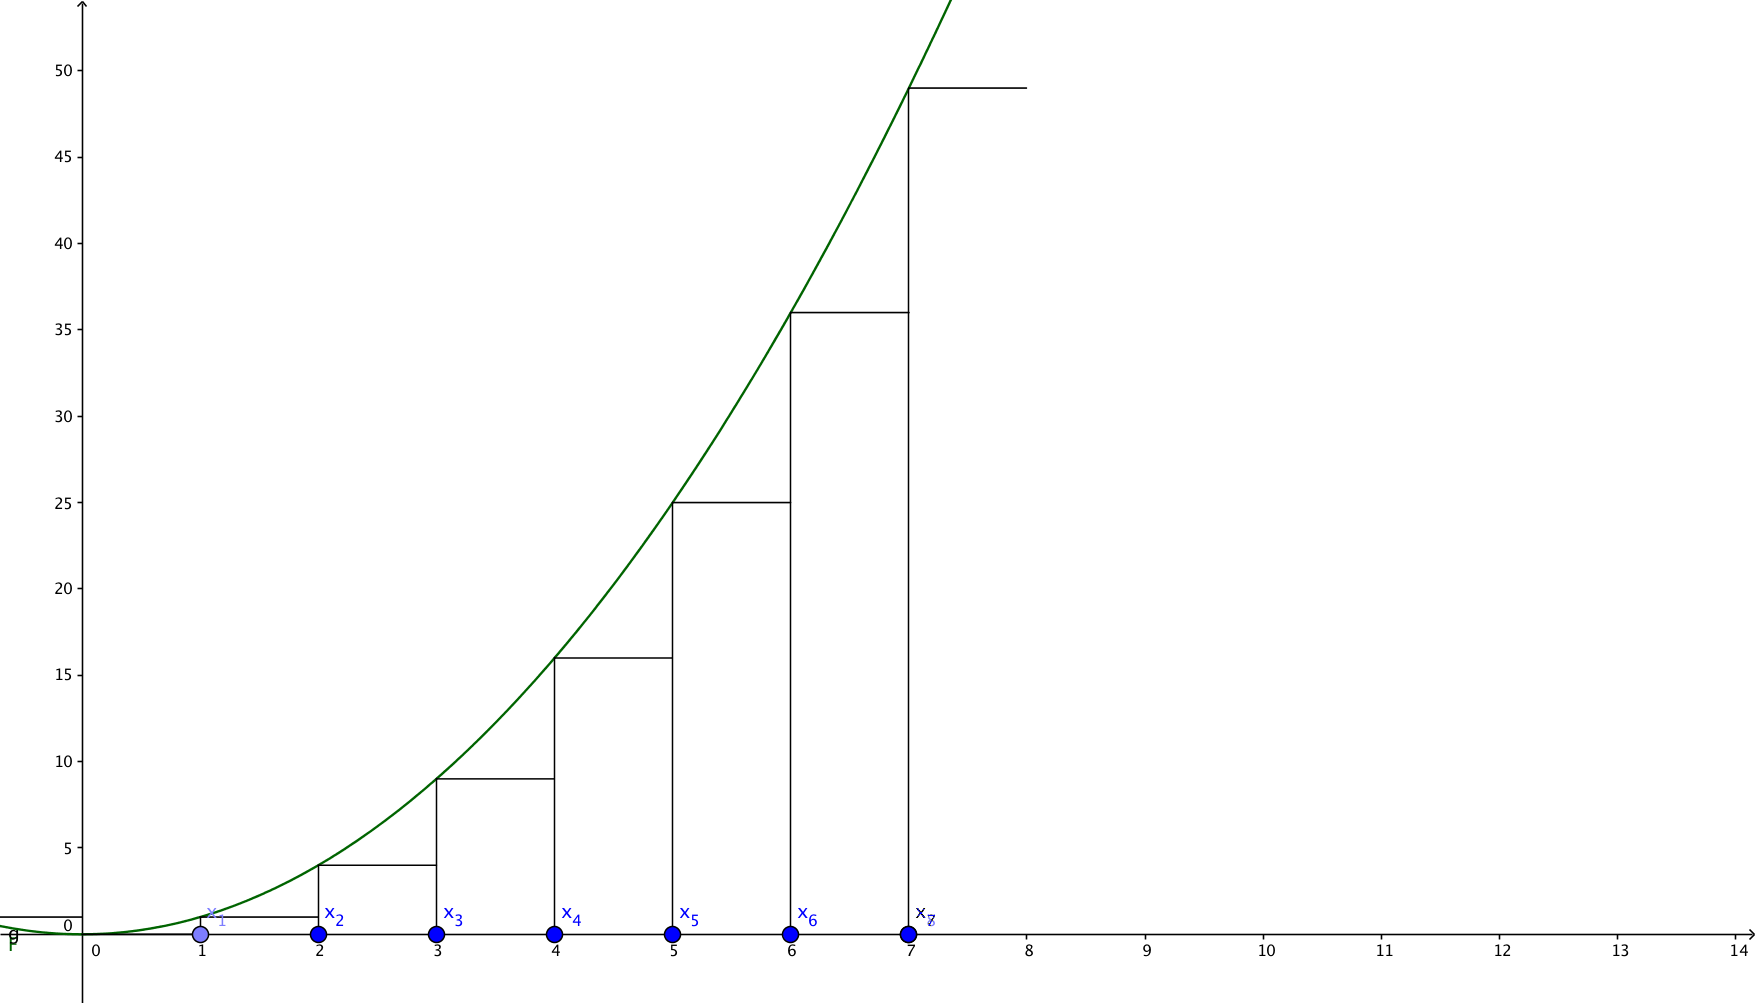
\includegraphics[width=8cm]{integral_quadratischefunktion}

	Für jedes einzelne Rechteck ($k=1, \ldots 6$) gilt mit $(x_{k+1} - x_{k}) = \frac{b-a}{N}$, wobei $a=x_{1}$ und $b=x_{N+1}$ ist:
	\begin{align*}
		W_{N}^{U}(k) & = F(x_{k}) \cdot (x_{k+1} - x_{k}) = F(x_{k}) \cdot \frac{b-a}{N} \\
		& = F\left((k-1)\frac{b-a}{N} + a\right) \frac{b-a}{N} \\
		& = \left( (k-1)^2\frac{(b-a)^2}{N^2} + 2(k-1) \frac{b-a}{N}a + a^2 \right) \frac{b-a}{N}
	\end{align*}}
\end{frame}

\begin{frame}{Integral quadratische Funktion}
\small{	Damit gilt für die gesamte Fläche (näherungsweise)
	\begin{align*}
		W_{N}^{U} & = \sum_{k=1}^{N} W(k) = \sum_{k=1}^{N} (k-1)^2 \frac{(b-a)^3}{N^3} + 2(k-1)\frac{(b-a)^2}{N^2}a + a^2 \frac{b-a}{N} \\
		&  = \sum_{k=0}^{N-1} k^2 \frac{(b-a)^3}{N^3} + 2k\frac{(b-a)^2}{N^2}a + a^2 \frac{b-a}{N} \\
		& = \frac{(b-a)^3}{N^3} \left( \sum_{k=0}^{N-1} k^2 \right)  + 2\frac{(b-a)^2}{N^2}a \left( \sum_{k=0}^{N-1} k \right) + a^2 (b-a) \\
		& = \frac{(b-a)^3}{N^3} \frac{N(N-1)(2N-1)}{6}  + 2\frac{(b-a)^2}{N^2}a \frac{N(N-1)}{2} + a^2 (b-a) \\
		& = \frac{(b-a)^3}{6N^3} \left( 2N^3 - 3N^2 + N \right) + \frac{(b-a)^2}{N^2} a (N^2 - N) +a^2 (b-a)
	\end{align*}
	Für $N \to \infty$ ist das
	\begin{align*}
		\lim_{N \to \infty} W_{N}^{U} & = \frac{(b-a)^3}{3} + (b-a)^2 a + a^2 (b-a) \\
		& = \frac{1}{3}b^3 - \frac{1}{3} a^3
  	\end{align*}}
\end{frame}

\begin{frame}{Grenzwerte oberer und unterer Treppenfunktionen}
	Für die untere Treppenfunktion gilt also:
	\[
		\lim_{N \to \infty} W_{N}^{U} = \frac{1}{3} b^3 - \frac{1}{3}a^3
	\]
	Entsprechend (ersetze $k-1$ durch $k$) gilt für die obere Treppenfunktion:
		\[
		\lim_{N \to \infty} W_{N}^{O} = \frac{1}{3} b^3 - \frac{1}{3}a^3
		\]
		
	Das heißt, die Fläche unter der Funktion $F(x)=x^2$ zwischen den Grenzen $a$ und $b$ ist $\frac{b^3 - a^3}{3}$.
\end{frame}

\subsection{Bestimmte Integrale}
\begin{frame}{Bestimmte Integrale}
	
	\begin{bemerkung}
		In der ausführlichen Rechnung tauchen immer fünf Dinge auf:
		\begin{itemize}
			\item ein Grenzwert ($N \to \infty$).
			\item ein Summenzeichen ($\sum_{k=1}^{N}$)
			\item die äußersten Grenzen $a$ und $b$
			\item die Funktionswerte an den Rechteckgrenzen (rechts oder links) $f(x_{k})$ bzw. $f(x_{k+1})$
			\item Die Breite der Rechtecke ($\Delta x_{k} = x_{k+1} - x_{k} = \frac{b-a}{N}$)
		\end{itemize}
		Also eigentlich ein Ausdruck der Form
		\[
			\lim_{N \to \infty}\sum_{k=1}^{N} F(x_{k}) \Delta x_{k}
		\]
	\end{bemerkung}
\end{frame}	
\begin{frame}{Stammfunktion}
	\begin{definition}
		Den o.g. Grenzwert bezeichnet man als \textbf{das bestimmte Integral von $f$ zwischen $a$ und $b$} und schreibt:
		\[
			\int_{a}^{b} f(x) dx
		\]
	\end{definition}
	\begin{definition}
		Definiert man die Funktion $F$ als
		\[
			F(x):=\int_{a}^{x} f(x) dx
		\]
		so erhält man eine \textbf{Integralfunktion} oder \textbf{Stammfunktion} von $f$.
		Insbesondere ist 
		\[
			\int_{0}^{x} x^2 dx = \frac{1}{3} x^3
		\] 
	\end{definition}
\end{frame}

\begin{frame}{Stammfunktionen und bestimmte Integrale}
	\begin{bemerkung}
		Hat man irgendeine Stammfunktion $F(x)$ zur Funktion $f(x)$ bestimmt, so ist für das bestimmte Integral
		\[
			\int_{a}^{b} f(x) dx = F(b) - F(a)
		\]
		Anschaulich bedeutet das, dass die Fläche zwischen den Grenzen $a$ und $b$ die Differenz derjenigen Fläche zwischen irgendeinem Wert $c$ und $b$ und der Fläche zwischen diesem Wert $c$ und $a$ ist.
		
		Man schreibt dann auch:
		\[
		\int_{a}^{b} f(x) dx = [F(x)]_{a}^{b} = F(x) |_{a}^{b} = F(b) - F(a)	
		\] 
		und bezeichnet $a$ als \textbf{untere Integrationsgrenze} und $b$ als \textbf{obere Integrationsgrenze}.
	\end{bemerkung}
\end{frame}

\begin{frame}{Geometrie des Integrals}
	\begin{bemerkung}
		Geometrisch ist das bestimmte Integral die Fläche zwischen den Grenzen $a$ und $b$, die die Funktion $f$ mit der x-Achse einschließt.
		
		Allerdings werden Flächenteile unterhalb der x-Achse negativ berechnet. Man muss also für die tatsächliche Fläche auf Vorzeichenwechsel der Funktion $f$ achten.
	\end{bemerkung}
\end{frame}

\subsection{Unbestimmte Integrale}

\begin{frame}{Unbestimmte Integrale}
	\begin{bemerkung}
		Hat man eine Stammfunktion $F(x)$ zur Funktion $f(x)$ bestimmt, so ist für jede konstante $C$ auch die Funktion $F_{C}(x) := F(x) + C$ eine Stammfunktion von $f(x)$, denn
		\[
			F_{C}'(x) = F'(x) = f(x)
		\]
		Es gibt also zu einer Funktion $f(x)$ unendlich viele Stammfunktionen.
		Da es egal ist, welche Stammfunktion man für die Berechnung der bestimmten Intgrale verwendet, bezeichnet man 
		\[
			\int f(x) dx = F(x) + C
		\]
		als das \textbf{unbestimmte Integral} der Funktion $f(x)$.
		Je zwei Stammfunktionen $F_{1}(x)$ und $F_{2}(x)$ zu einer Funktion $f(x)$ können sich höchstens um eine Konstante unterscheiden, weil
		\[
			F_{1}'(x) - F_{2}'(x) = f(x) - f(x) = 0
		\]
	\end{bemerkung}
\end{frame}

\subsection{Elementare Stammfunktionen}

\begin{frame}{Elementare Stammfunktionen}
\footnotesize{
	\begin{example}
		\begin{align*}
			\int 2x dx & = x^2 +C \\
			\int \frac{1}{2\sqrt{x}} dx & = \sqrt{x} + C \\
			\int \frac{1}{x} dx & = \ln |x| + C \\
			\int e^{x} dx & = e^{x} + C \\
			\int x^{\alpha} dx & = \frac{1}{\alpha + 1} x^{\alpha + 1} + C \qquad \forall \alpha \in \mathbb{R} \setminus \{ -1 \} \\
			\int a^{x} dx & = \frac{1}{\ln a} a^{x} + C \\
			\int \sin (x) dx & = - \cos (x) + C \\
			\int \cos (x) dx & = \sin (x) +C \\
			\int \frac{1}{1+x^{2}} dx & = \arctan x + C
		\end{align*}	
	\end{example}}
\end{frame}

\subsection{Integrationsregeln}

\begin{frame}{Integrationsregeln}
	\begin{bemerkung}
		So, wie es für die Ableitung bestimmte Regeln und Sätze gibt, die angeben, wie man die Ableitung zusammengesetzter Funktionen berechnen kann, gibt es Regeln für die Bestimmung von Integralen. 
		
			Wir werden uns im Folgenden mit diesen Regeln befassen:
			\begin{itemize}
				\item Faktorregel
				\item Summen- und Differenzenregel
				\item Partielle Integration
				\item Integration durch Substitution
				\item Logarithmische Integration
				\item Partialbruchzerlegung
			\end{itemize}
	\end{bemerkung}
\end{frame}

\subsection{Faktor-, Summen- und Differenzenregel}
\begin{frame}{Faktor-, Summen- und Differenzenregel}
	\begin{theorem}
		Für das (un-)bestimmte Integral zweier Funktionen $f(x)$ und $g(x)$ gilt:
		\begin{align*}
			\int k f(x) dx & = k \int f(x) dx \qquad \forall k \in \mathbb{R} & \text{  Faktorregel} \\
			\int f(x) + g(x) dx & = \int f(x) dx + \int g(x) dx & \text{  Summenregel}\\
			\int f(x) - g(x) dx & = \int f(x) dx - \int g(x) dx & \text{  Differenzenregel}\\
		\end{align*}
		Die Faktor- und die Summenregel fasst man auch zusammen unter dem Begriff der \textbf{Linearität des Integrals}
	\end{theorem}
\end{frame}

\begin{frame}{Intervallzerlegung}
	\begin{bemerkung}
		Für $a \leq b \leq c$ und eine integrierbare Funktion $f$ gilt:
		\[
			\int_{a}^{c} f(x) dx = \int_{a}^{b} f(x) dx + \int_{b}^{c} f(x) dx
		\]
		
		Für die Fläche $A$ zwischen x-Achse und der Funktion $f(x)$ gilt:
		\begin{align*}
			A = \int_{a}^{b} f(x) dx \geq 0 & \text{ falls } f(x) \geq 0 \qquad\forall x\in [a, b] \\
			A = - \int_{a}^{b} f(x) dx \geq 0 & \text{ falls } f(x) \leq 0 \qquad \forall x\in [a, b]
		\end{align*}
	\end{bemerkung}
\end{frame}

\begin{frame}{Symmetrieeigenschaften des Integrals}
	\begin{bemerkung}
		Für eine gerade Funktion $f(x)$ (also $f(-x) = f(x) \quad \forall x$) gilt:
		\[
			\int_{-a}^{a} f(x) dx = 2 \int_{0}^{a} f(x) dx
		\]

		Für eine ungerade Funktion $f(x)$ (also $f(-x) = -f(x) \quad \forall x$) gilt:
		\[
			\int_{-a}^{a} f(x) dx = 0
		\]
		
		Für das bestimmte Integral gilt allgemein:
		\begin{align*}
			\int_{a}^{b} f(x) dx & = - \int_{b}^{a} f(x) dx \\
			\left| \int_{a}^{b} f(x) dx \right| & \leq \int_{a}^{b} | f(x) | dx
		\end{align*}

	\end{bemerkung}
\end{frame}

\subsection{Partielle Integration}

\begin{frame}{Partielle Integration}
\begin{bemerkung}
	Für die Ableitung einer differenzierbaren Funktion $h(x)=f(x)\cdot g(x)$ gilt die Produktregel:
	\[
		h'(x) = (f\cdot g)'(x) = f'(x)\cdot g(x) + f(x) \cdot g'(x) 
	\]
	Das bedeutet für die Funktion $h$ als Stammfunktion von $h'$ 
	\small{\begin{align*}
		& \int_{a}^{b} h'(x) dx = \left[ (f(x) \cdot g(x)) \right]_{a}^{b} = \int_{a}^{b} f'(x) \cdot g(x) dx + \int_{a}^{b} f(x)\cdot g'(x) dx \\
		& \Leftrightarrow \int_{a}^{b} f(x)\cdot g'(x) dx = [f(x)\cdot g(x)]_{a}^{b} - \int_{a}^{b} f'(x)\cdot g(x) dx
 	\end{align*}}
\end{bemerkung}
\end{frame}

\begin{frame}{Partielle Integration}
\begin{theorem}[Partielle Integration]
	Für das bestimmte Integral gilt:
	\[
		\int_{a}^{b} f(x)\cdot g'(x) dx = f(x)\cdot g(x) |_{a}^{b} - \int_{a}^{b} f'(x) \cdot g(x) dx
	\]
	
	Für das unbestimmte Integral gilt entsprechend:
	\[
		\int f(x)\cdot g'(x) dx = f(x)\cdot g(x) - \int f'(x) \cdot g(x) dx
	\]
\end{theorem}
\begin{bemerkung}
	Der Satz ist dann nützlich, wenn man das Produkt zweier Funktionen integrieren möchte und die Stammfunktion $g(x)$ des einen Faktors (hier $g'(x)$) kennt. Man wälzt dann mit diesem Satz die Ableitung des Fakt $g'(x)$ auf $f(x)$; oft vereinfacht das die Integration. 
\end{bemerkung}
\end{frame}

\begin{frame}{Beispiele zur partiellen Integration}
	\begin{example}
		Für die Stammfunktion der Funktion $h(x)=x\cdot e^{x}$ gilt mit $f(x)=x$ und $g'(x)=e^{x}$:
		\begin{align*}
			\int x e^{x} dx & = x \cdot e^{x} - \int 1 \cdot e^{x} dx = x \cdot e^{x} - e^{x} + C = (x-1) \cdot e^{x} + C
 		\end{align*}
	\end{example}
	\begin{example}
		Für die Stammfunktion der Funktion $h(x)=x^{2} \cdot \ln x$ gilt mit $f'(x)=x^{2}$ und $g(x)=\ln x$:
		\begin{align*}
			\int x^2 \ln x dx & = \frac{1}{3}x^{3} \cdot \ln x - \int \frac{1}{3}x^{3} \cdot \frac{1}{x}dx \\ 
				& = \frac{1}{3}x^{3} \ln x - \frac{1}{3} \int x^{2} dx \\ 
				& = \frac{1}{3}x^{3} \ln x - \frac{1}{9} x^{3} + C
 		\end{align*}
	\end{example}
	
\end{frame}

\begin{frame}{Beispiele zur partiellen Integration}
\begin{example}
	Für die Stammfunktion der Funktion $h(x)=(3x-7)\cdot e^{-x}$ gilt mit $f(x)=3x+7$ und $g'(x)=e^{-x}$:
		\begin{align*}
			\int (3x-7) \cdot e^{-x} dx & = (3x-7)\cdot (-e^{-x}) - \int 3 \cdot (-e^{-x}) dx \\
			& = (3x-7)\cdot (-e^{-x}) + 3 \int e^{-x} dx \\
			& = (3x-7)\cdot (-e^{-x}) - 3 e^{-x} + C\\
			& = (4-3x)\cdot e^{-x} +C
		\end{align*}
\end{example}
\end{frame}

\begin{frame}{Beispiele zur partiellen Integration}
\begin{example}
	Für die Stammfunktion der Funktion $h(x)=x \cos x$ gilt mit $f(x)=x$ und $g'(x)=\cos x$:
	\begin{align*}
		\int x \cos x \, dx & = x \sin x - \int 1 \cdot \sin x \, dx \\
		& = x \sin x + \cos x + C 
	\end{align*}
\end{example}
\end{frame}

\begin{frame}{Beispiele zur partiellen Integration}
\small{	
	\begin{example}
		Für das Integral der Funktion $h(x)= \sin^{2} x$ gilt mit $f(x)=\sin x$ und $g'(x)= \sin x$:
		\begin{align*}
			\int \sin^{2} x \, dx & = \int \sin x \cdot \sin x \, dx = -\sin x \cdot \cos x + \int \cos x \cdot \cos x \, dx \\
			& = -\sin x \cdot \cos x + \int \cos^{2} x \, dx \\ 
			& = -\sin x \cdot \cos x + \int 1-\sin^{2} x \, dx\\
			& = -\sin x \cdot \cos x + x - \int \sin^{2} x \, dx \\
			\Leftrightarrow 2\cdot \int \sin^{2} x\, dx & = -\sin x \cdot \cos x + x \\
			\Leftrightarrow  \int \sin^{2} x\, dx & = -\frac{1}{2}\sin x \cdot \cos x + \frac{x}{2}
		\end{align*}
	\end{example}}
\end{frame}

\subsection{Integration durch Substitution}
\begin{frame}{Integration durch Substitution}
\begin{bemerkung}
\footnotesize{	Die Kettenregel für die Ableitung einer Funktion $h(x)=f(g(x))$ lautet:
	\[
		h'(x) = f'(g(x)) \cdot g'(x)
	\]
	Wir hatten das auch mal so geschrieben:
	\[
		\frac{dh}{dx}(x) = \frac{df}{dg}(g(x)) \cdot \frac{dg}{dx}(x)
	\]
	oder noch einfacher (wenn man nicht vergisst, an welchen Stellen man die Funktionen auswertet):
	\[	
		\frac{dh}{dx} = \frac{df}{dg} \cdot \frac{dg}{dx}
	\]
	Integriert man das, so erhält man
	\begin{align*}
		\int \frac{dh}{dx} dx  & = \int \frac{df}{dg} \cdot \frac{dg}{dx} dx \\
		\Leftrightarrow h(x) & = \int \frac{df}{dg} \cdot dg = f(g) = f(g(x))
	\end{align*}
	Es genügt also in diesem Fall, die Stammfunktion $f$ als Funktion von $g$ zu kennen. }
\end{bemerkung}
\end{frame}

\begin{frame}{Integration durch Substitution}
\begin{bemerkung}
	Sind $f$ und $g$ stetige Funktionen und $F$ eine Stammfunktion von $f$, so gilt offenbar nicht nur $F'(x)=f(x)$, sondern (wegen der Kettenregel) auch:
	\[
		\left(F(g(x)\right)' = F'(g(x))\cdot g'(x) = f(g(x))\cdot g'(x)
	\]
	Also ist $F(g(x))$ eine Stammfunktion von $f(g(x))\cdot g'(x)$
\end{bemerkung}
\begin{theorem}
	Ist $f(x)$ stetig und $g(x)$ eine stetig differenzierbare, umkehrbare Funktion, dann gilt:
	\[
		\int_{a}^{b} f(x) dx = \int_{g^{-1}(a)}^{g^{-1}(b)} f(g(t)) g'(t) dt = \int_{g^{-1}(a)}^{g^{-1}(b)} f(g) dg
	\]
	Wichtig ist, dass sich auch die Integrationsgrenzen ändern, weil man ja die Integrationsvariable ersetzt hat.
\end{theorem}
\end{frame}


\begin{frame}{Beispiele - Integration durch Substitution}
\begin{example}
Für das Integral
\[
	\int \frac{1}{x+a}dx
\]	
erhält man mit $g(x)=x+a$ und $\frac{dg}{dx}=1$, also $dg=dx$ und daher
\[
\int \frac{1}{x+a}dx = \int \frac{1}{g} dg = \ln |g| + C= \ln |x+a| +C
\]
\end{example}
\begin{example}
	Für das Integral $\int \frac{2x}{x^2+1} dx$ erhält man mit $g(x)=x^2+1$ und $\frac{dg}{dx}= 2x$, also $dg = 2x\,dx$ dann
	\[
		\int \frac{2x}{x^2+1} dx = \int \frac{1}{g}dg = \ln |g| + C = \ln |x^2+1| +C
	\]
\end{example}
\end{frame}

\begin{frame}{Beispiel - Integration durch Substitution}
\begin{example}
	Für das Integral $\int x \cos (x^{2})\,dx$
	\begin{itemize}
		\item substituiert man zuerst $g(x)=x^{2}$, also $x=\sqrt{g}$. Aus dem Integranden wird damit 
			\[
				x \cos (x^{2}) \rightarrow \sqrt{g} \cos (g)
			\]
			\item und für das Differential $dx$ ersetzt man 
			\[
				\frac{dg}{dx} = 2x \quad \Leftrightarrow \quad dx = \frac{dg}{2x} = \frac{dg}{2\sqrt{g}} 
			\]
		\item Für das Integral schreibt man dann also
		\[
			\int x \cos (x^{2}) dx = \int \sqrt{g} \cos (g) \frac{dg}{2 \sqrt{g}} = \frac{1}{2}\int \cos (g) dg = \frac{1}{2}\sin(x^{2})
		\]
	\end{itemize}
\end{example}
\end{frame}


\begin{frame}{Beispiel - Integration durch Substitution}
\begin{example}
	Da $\tan x = \frac{\sin x}{\cos x}$ ist, kann man mit $g(x)=\cos x$ und $\frac{dg}{dx}= -\sin x$, also $dg = -\sin x \,dx$ rechnen:
	\[
		\int \tan x \, dx = \int \frac{\sin x}{\cos x} dx = - \int \frac{dg}{g} = -\ln |g| +C = -\ln |\cos x| + C
	\]
\end{example}
\end{frame}

\subsection{Logarithmische Integration}
\begin{frame}{Logarithmische Integration}
\begin{bemerkung}
	Das vorletzten Beispiele sind Spezialfälle der folgenden, allgemeinen Beobachtung:
	Für die Ableitung einer Funktion $h(x)=\ln |f(x)|$ gilt wegen der Kettenregel:
	\[
		h'(x)=\frac{f'(x)}{f(x)}
	\]
	Damit gilt für das Integral
	\[
		\int \frac{f'(x)}{f(x)}dx = \ln |f(x)| + C
	\]
\end{bemerkung}
\end{frame}

\subsection{Integration durch Partialbruchzerlegung}
\begin{frame}{Integration von rationalen Funktionen}
	\begin{bemerkung}
	\begin{itemize}
		\item \textbf{Die gute Nachtricht:} Mit den bisherigen Methoden können Sie für jede rationale Funktion eine Stammfunktion bestimmen.
		\item \textbf{Die schlechte Nachricht:} In einigen Fällen ist das ziemlich aufwendig.
	\end{itemize}
	\end{bemerkung}
\small{	\begin{example}
		Für die einfachste rationale Funktion gilt
		\[	
			\int \frac{1}{x} dx = \ln |x| +C
		\]
		und daher auch
		\[
			\int \frac{1}{ax+b} dx = \frac{1}{a} \ln |ax+b| + C
		\]
		und speziell
		\[
			\int \frac{1}{x-x_{0}} dx = \ln |x-x_{0}| + C
		\]
	\end{example}}
\end{frame}

\begin{frame}{Integration von rationalen Funktionen}
	\small{\begin{example}
		Für $k\neq -1 $ ist
		\[
			\int \frac{1}{x^{k}} dx = \int x^{-k} dx = \frac{x^{-k+1}}{-k+1} + C = \frac{1}{(1-k)x^{k-1}} + C
		\]	
		und mit Substitution auch
		\[
			\int \frac{1}{(ax+b)^{k}} dx = \frac{(ax+b)^{-k+1}}{a(-k+1)} +C = \frac{1}{a(1-k)(ax+b)^{k-1}} +C
		\]
		und damit auch
		\[
			\int\frac{1}{(x-x_{0})^{k}}dx = \frac{1}{-k+1}(x-x_{0})^{-k+1} + C = \frac{1}{-k+1}\frac{1}{(x-x_{0})^{k-1}} +C 
		\]
		Damit ist zum Beispiel
		\[
			\int \frac{1}{x^2 +6x +9} dx = \int \frac{1}{(x+3)^{2}}dx = \frac{-1}{x+3} +C
		\]
	\end{example}
}	
\end{frame}

\begin{frame}{Integration von rationalen Funktionen}
	\small{\begin{example}
		Für die Stammfunktion von $\frac{1}{x^2 + 1}$ gilt:
		\[
			\int \frac{1}{x^2+1} dx = \arctan x + C	
		\]
		Denn mit der Substitution $x= \tan z$ und damit auch $dx = (1+\tan^{2}z ) dz$ ist  
		\begin{align*}
			\int \frac{1}{1+x^2}dx = \int \frac{1}{1+\tan^{2}z} (1+\tan^{2}z)dz = \int 1 dz = z+ C = \arctan x + C
		\end{align*}
	\end{example}
}
\end{frame}


\begin{frame}{Partialbruchzerlegung}
\begin{bemerkung}
		Für eine gebrochen-rationale Funktion $f$ mit
		\[
			f(x)=\frac{g(x)}{h(x)} = \frac{a_{m}x^{m} + a_{m-1}x^{m-1} + \ldots a_{2}x^{2}+a_{1}x + a_{0}}{b_{n}x^{n} + b_{n-1}x^{n-1} + \ldots b_{2}x^{2}+b_{1}x + b_{0}}
		\]
		kann man den Nenner zerlegen in Linearfaktoren für jede Nullstelle des Nenners, und weitere Terme, die (Potenzen) quadratischer Polynome sind, sowie einen konstanten Vorfaktor, also
		\[
			h(x)=b_{n}(x-x_{1})^{k_{1}}(x-x_{2})^{k_{2}}\cdot \ldots \cdot (x-x_{r})^{k_{r}}\cdot q_{1}^{l_{1}}\cdot \ldots \cdot q_{s}^{l_{s}}
		\]
\end{bemerkung}
\end{frame}

\begin{frame}{Partialbruchzerlegung - Fortsetzung}
\begin{bemerkung}		
		Die \textbf{Partialbruchzerlegung von $f$} ist dann
		\begin{align*}
			f(x) & = \frac{A_{11}}{x-x_{1}} + \frac{A_{12}}{(x-x_{1})^{2}} + \ldots + \frac{A_{1k_{1}}}{(x-x_{1})^{k_{1}}}  \\
			& + \frac{A_{21}}{x-x_{2}} + \frac{A_{22}}{(x-x_{2})^{2}} + \ldots + \frac{A_{2k_{2}}}{(x-x_{2})^{k_{2}}}  \\
			& + \frac{A_{r1}}{x-x_{r}} + \frac{A_{r2}}{(x-x_{r})^{2}} + \ldots + \frac{A_{rk_{2}}}{(x-x_{2})^{k_{r}}}  \\
			& + \frac{B_{11}x+C_{11}}{q_{1}(x)} + \frac{B_{12}x+C_{12}}{(q_{1}(x))^{2}} + \ldots + \frac{B_{1l_{1}}x+C_{1l_{1}}}{(q_{1}(x))^{l_{1}}} \\
			& + \ldots \\
			& + \frac{B_{s1}x+C_{s1}}{q_{s}(x)} + \frac{B_{s2}x+C_{s2}}{(q_{s}(x))^{2}} + \ldots + \frac{B_{sl_{s}}x+C_{sl_{s}}}{(q_{s}(x))^{l_{s}}}
		\end{align*}
	\end{bemerkung}
\end{frame}

\subsection{Uneigentliche Integrale}
\begin{frame}{Uneigentliche Integrale}
	\begin{definition}
		Falls die Grenzwerte auf der rechten Seite der folgenden Gleichungen existieren, so bezeichnet man die folgenden Integrale als \textbf{uneigentliche Integrale} ($x_{0}$ ist eine Polstelle):
		\begin{align*}
			\int_{a}^{\infty} f(x) dx & := \lim_{b \to \infty} \int_{a}^{b}f(x) dx \\ 
			\int_{-\infty}^{b} f(x) dx & := \lim_{a \to -\infty} \int_{a}^{b}f(x) dx \\
			\int_{-\infty}^{\infty} f(x) dx & := \lim_{a \to -\infty} \lim_{b \to \infty} \int_{a}^{b}f(x) dx \\
			\int_{x_{0}}^{b} f(x) dx & := \lim_{\varepsilon \to 0} \int_{x_{0}+\varepsilon}^{b}f(x) dx \\
			\int_{a}^{x_{0}} f(x) dx & := \lim_{\varepsilon \to 0} \int_{a}^{x_{0}-\varepsilon}f(x) dx 
		\end{align*}	
	\end{definition}
\end{frame}

\begin{frame}{Uneigentliche Integrale - Beispiel}	
	\begin{example}
		Die Funktion $f(x)=\frac{1}{\sqrt{x}}=x^{-\frac{1}{2}}$ hat an der Stelle $x_{0}=0$ eine Polstelle.
		Für das (bestimmte) Integral und $a, b \geq 0$ gilt:
		\[
			\int_{a}^{b} \frac{1}{x^{\frac{1}{2}}} dx = [ 2 x^{\frac{1}{2}} ]_{a}^{b} = 2 ( \sqrt{b} - \sqrt{a} )
		\]	
		Insbesondere gilt:
		\[
			\int_{0}^{1} \frac{1}{x^{\frac{1}{2}}} dx = [ 2 x^{\frac{1}{2}} ]_{0}^{1} = 2 ( \sqrt{1} - \sqrt{0} ) = 2
		\]
%		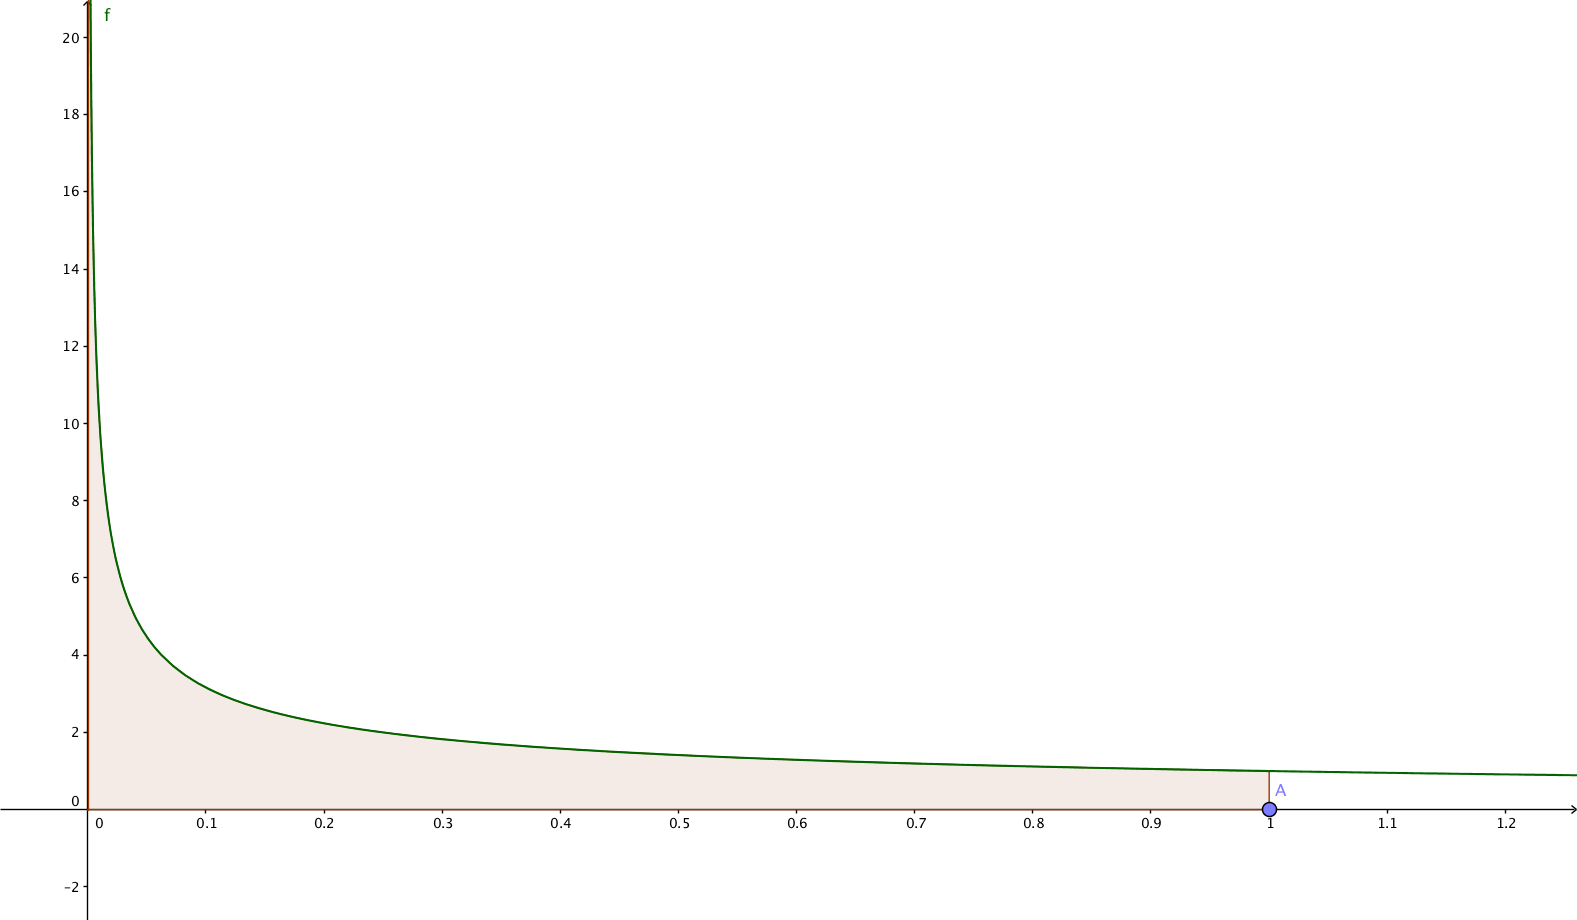
\includegraphics[width=3cm]{integral_uneigentlich}
	\end{example}
\end{frame}

\begin{frame}{Uneigentliche Integrale - Beispiel}	
	\begin{example}
		Die Funktion $f(x)=\frac{1}{x^{2}}=x^{-2}$ konvergiert für $x \to \infty$ gegen $0$.
		Für das (bestimmte) Integral und $a, b \geq 0$ gilt:
		\[
			\int_{a}^{b} \frac{1}{x^2} dx = [ - \frac{1}{x} ]_{a}^{b} =  \frac{1}{a} - \frac{1}{b}
		\]	
		Insbesondere gilt:
		\[
			\int_{1}^{\infty} \frac{1}{x^{2}} dx = \frac{1}{1} - \lim_{b \to \infty}\frac{1}{b} = 1
		\]
	\end{example}
\end{frame}

\begin{frame}{Uneigentliche Integrale - Beispiele}
\begin{example}
\scriptsize{	Die Gammafunktion $\Gamma (x)$, die u.a. in der Statistik eine wichtige Rolle spielt, ist durch das uneigentliche Integral 
	\[
		\Gamma (x) := \int_{0}^{\infty} t^{x-1}e^{-t}\,dt \text{ für } x > 0 
	\]
	definiert.
	Für $\Gamma (x+1)$ erhält man mittels partieller Integration
	\begin{align*}
		\Gamma (x+1) & = \int_{0}^{\infty} t^{x}e^{-t}\, dt = \lim_{b \to \infty} \int_{0}^{b} t^{x}e^{-t}\, dt \\
		& = - \lim_{b \to \infty} \int_{0}^{b} t^{x}(e^{-t})' \, dt \\
		&= - \lim_{b \to \infty} [t^{x}e^{-t}]_{0}^{b} + \int_{0}^{b} (t^{x})' e^{-t}\, dt \\
		&= - \lim_{b \to \infty} b^{x}e^{-b} + \int_{0}^{b} xt^{x-1} e^{-t}\, dt \\
		&= 0 + \lim_{b \to \infty} x\int_{0}^{b} t^{x-1} e^{-t}\, dt = x\Gamma (x)
	\end{align*}
	Wegen $\Gamma (1)=\lim_{b \to \infty} \int_{0}^{b} e^{-t}\,dt = \lim_{b \to \infty} [-e^{-t}]_{0}^{b} = 1$ ist damit 
	\[
	\Gamma (x+1) = x \Gamma (x) = x (x-1) \Gamma(x-2) = x (x-1) (x-2) \ldots 2 \cdot 1 = x!
	\]}
\end{example}
\end{frame}

\subsection{Anwendungen der Integralrechnung}
\subsubsection{Länge von Kurven}
\begin{frame}{Längenberechnung von Kurven}
\begin{definition}
	Für die Länge einer durch eine Funktion $f(x)$ gegebene Kurve zwischen den Stellen $a$ und $b$ gilt:
	\[
		s_{a}^{b}(f) = \int_{a}^{b} \sqrt{1+(f'(x))^{2}}\, dx  
	\]
\end{definition}
\end{frame}

\begin{frame}{Längenberechnung von Kurven - Beispiel}
\begin{example}
\small{	Für die Länge eines Halbkreises mit Radius $R$, der durch die Funkion $f(x)=\sqrt{R^2-x^2}$ dargestellt werden kann, gilt:
	\begin{align*}
		s_{-R}^{R}(f) & = \int_{-R}^{R} \sqrt{1+(f(x)')^{2}}\, dx \\
		& = \int_{-R}^{R} \sqrt{1+\left( -\frac{x}{\sqrt{R^2-x^2}} \right)^{2}}\, dx \\
		& = \int_{-R}^{R} \sqrt{1+\frac{x^2}{R^2-x^2}}\, dx = \int_{-R}^{R} \sqrt{\frac{R^2}{R^2-x^2}}\, dx \\
		& = \int_{-R}^{R} \frac{R}{\sqrt{R^2-x^2}}\, dx = \left[ R \arcsin \frac{x}{R} \right]_{-R}^{R} \\
		& = 2 R \arcsin(1) = R \pi	
	\end{align*}}
\end{example}
\end{frame}

\subsubsection{Rotationskörper}
\begin{frame}{Volumen von Rotationskörpern}
\begin{definition}
	Für die Volumen eines durch Rotation einer Funktion $f(x)$ zwischen den Stellen $a$ und $b$ berandeten Körpers  gilt:
	\[
		V_{a}^{b}(f) = \pi \int_{a}^{b} (f(x))^{2} \, dx  
	\]
	Für die Mantelfläche desselbe Rotationskörpers gilt:
	\[
		O_{a}^{b}(f) = 2\pi \int_{a}^{b} f(x) \sqrt{1+(f'(x))^2}\, dx
	\]
\end{definition}
\end{frame}

\begin{frame}{Rotationskörper - Beispiel}
\small{	\begin{example}
		Ein Kegelstumpf der Höhe $h$ und mit den Deckelradien $r$ und $R$ kann beschrieben werden durch Rotation der linearen Funktion $f(x)= \frac{R-r}{h} \cdot x + r$ um die x-Achse (für $a=0$ und $b=h$ gilt dann $f(a)=f(0)=r$ und $f(b)=f(h)=R$).
		Für das Volumen des Kegelstumpfes gilt dann
		\begin{align*}
			V & = \pi \int_{0}^{h} \left( f(x) \right)^2 \, dx \\
			& = \pi \int_{0}^{h} \left( \frac{R-r}{h} x +r \right)^{2}\, dx \\
			& = \pi \int_{0}^{h} \frac{(R-r)^2}{h^2} x^2  +2 \frac{R-r}{h}xr +r^2 \, dx \\
			& = \pi \left[ \frac{(R-r)^2}{3h^2} x^3  + \frac{R-r}{h}rx^{2} +r^2 x \right]_{0}^{h}\, dx \\
			& = \pi \frac{(R-r)^2}{3}h + (R-r)hr + r^2 h = \frac{h \pi}{3} (R^2 + Rr +r^2 ) 
		\end{align*}
	\end{example}}
\end{frame}




%\section*{Anhang}
%\begin{frame}{Hinweis}
%	Diese Folien sind nicht vollständig und werden noch immer verändert und erweitert!
%\end{frame}

\end{document}

